\documentclass[12pt,oneside,openany,a4paper, %... Layout
english, %... Global lang drivers{}
masters-t, goldenblock]{usthesis} 
\usepackage{float} %for images
\usepackage{graphicx}
\usepackage{cite}
% \usepackage[colorinlistoftodos,prependcaption,textsize=small,disable]{todonotes}
\usepackage[colorinlistoftodos,prependcaption,textsize=small]{todonotes}
\usepackage{pgfgantt}
\usepackage{float} %so that it can use the 'f' float option
\usepackage{pdflscape} %allow you to make landscape pages
\usepackage{amsmath}
\newcommand*\mean[1]{\bar{#1}} % to create an overbar for symbols
% \usepackage{cite}
\usepackage{soul}
\usepackage{amssymb}
\usepackage{bm}
\usepackage{standalone}
\usepackage{subcaption} %for multiple images in one figure
% \usepackage{subfig} %for multiple images in one figure
\usepackage{preview}
\usepackage{mathtools}
\usepackage{pdfpages}
\usepackage{enumitem}
\setlistdepth{9}
% \usepackage[sort&compress]{natbib} %able to cite 2 reference at once
\usepackage[toc,page]{appendix} % for appendices
\allowdisplaybreaks %allow equations to over multiple pages
\usepackage{xspace}
\newcommand{\MATLAB}{\textsc{Matlab}\xspace} %writing the Matlab symbol


% \usepackage[latin1]{inputenc}
\usepackage{tikz}
\usetikzlibrary{shapes,arrows,positioning}

%command for capitalised roman numerals
\newcommand{\RomanNumeralCaps}[1]
    {\MakeUppercase{\romannumeral #1}}


% \usepackage{gensymb} %for degree symbol
% \usepackage{hyperref} %to hyperlink the equations

%packages required by matlab2tikz function
\usepackage{pgfplots}
\pgfplotsset{compat=newest}
%% the following commands are needed for some matlab2tikz features
\usetikzlibrary{plotmarks}
\usetikzlibrary{arrows.meta}
\usepgfplotslibrary{patchplots}
\usepackage{grffile}
% \usepackage{amsmath}
\usepackage[framed,numbered,autolinebreaks,useliterate]{mcode} % for inserting matlab code


\usepackage{listings} %For code in appendix
\lstset
{ %Formatting for code in appendix
    language=Matlab,
    basicstyle=\footnotesize,
    numbers=left,
    stepnumber=1,
    showstringspaces=false,
    tabsize=1,
    breaklines=true,
    breakatwhitespace=false,
}

\newganttlinktype{drur}{
\ganttsetstartanchor{on bottom=0.75}
\ganttsetendanchor{on left}
\draw [/pgfgantt/link]
% first segment (down)
(\xLeft, \yUpper) --
% second segment (right)
(\xLeft, \yUpper -
\ganttvalueof{link bulge} * \ganttvalueof{y unit chart}) --
% link label
node [pos=.5, /pgfgantt/link label anchor] {\ganttlinklabel}
% third segment (up)
($(\xLeft,
\yUpper -
\ganttvalueof{link bulge} * \ganttvalueof{y unit chart})!%
\ganttvalueof{link mid}!%
(\xRight,
\yUpper -
\ganttvalueof{link bulge} * \ganttvalueof{y unit chart})$) --
% last segment (right again)
($(\xLeft, \yLower)!%
\ganttvalueof{link mid}!%
(\xRight, \yLower)$) --
(\xRight, \yLower);
}

\newganttlinktype{rdldr*}{%
  \draw [/pgfgantt/link]
    (\xLeft, \yUpper) --
    (\xLeft + \ganttvalueof{link bulge 1} * \ganttvalueof{x unit},
      \yUpper) --
    ($(\xLeft + \ganttvalueof{link bulge 1} * \ganttvalueof{x unit},
      \yUpper)!%
      \ganttvalueof{link mid}!%
      (\xLeft + \ganttvalueof{link bulge 1} * \ganttvalueof{x unit},
      \yLower)$) --
    ($(\xRight - \ganttvalueof{link bulge 2} * \ganttvalueof{x unit},
      \yUpper)!%
      \ganttvalueof{link mid}!%
      (\xRight - \ganttvalueof{link bulge 2} * \ganttvalueof{x unit},
      \yLower)$) --
    (\xRight - \ganttvalueof{link bulge 2} * \ganttvalueof{x unit},
      \yLower) --
    (\xRight, \yLower);%
}
\ganttset{
  link bulge 1/.link=/pgfgantt/link bulge,
  link bulge 2/.link=/pgfgantt/link bulge}

\begin{document}

\includepdf{Cover.pdf}
% 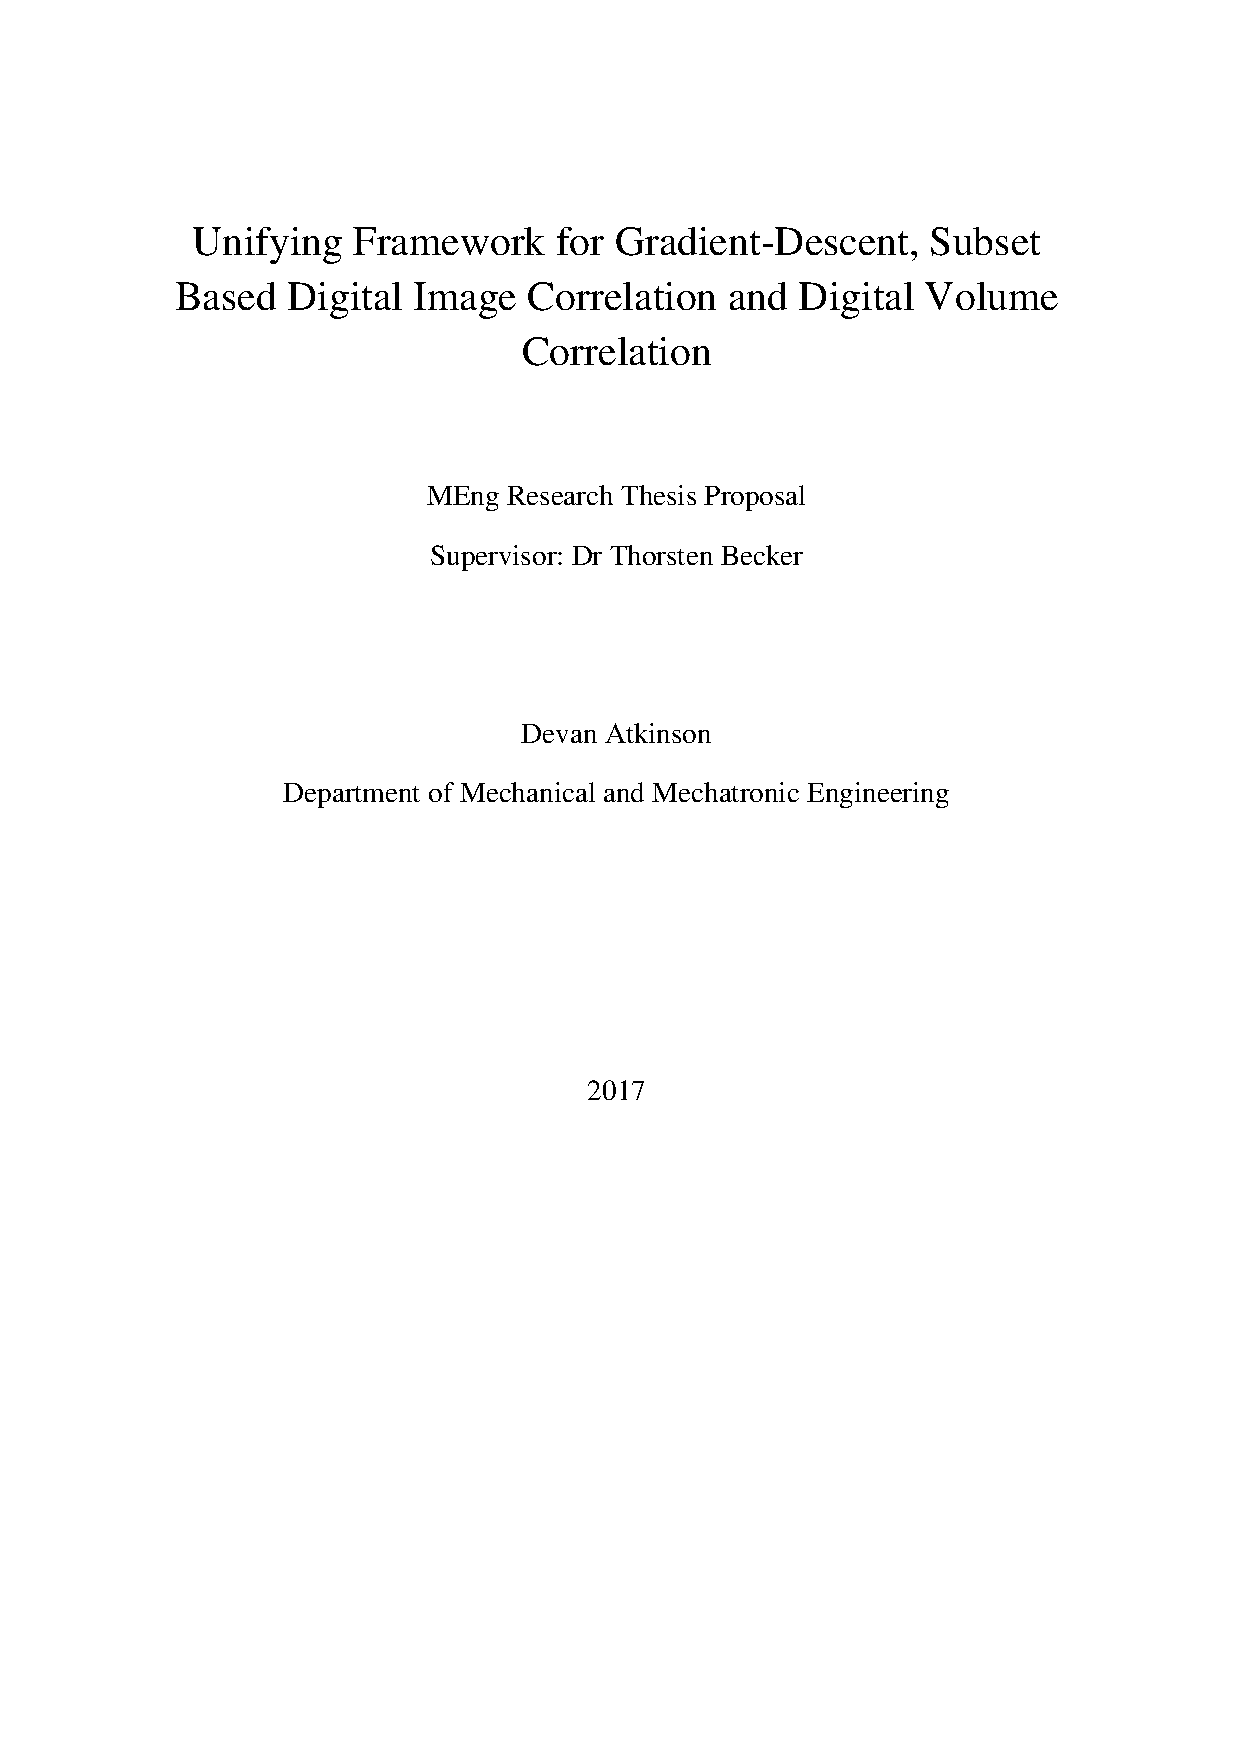
\includepdf{TitlePage.pdf}

\includepdf{plagiarism_signed.pdf}
% \chapter*{Abstract}
% Digital Image Correlation (DIC) and Digital Volume Correlation (DVC) are becoming widely used tools, in the field of material science, to measure the displacements and deformations of specimens. However the high cost of commercial DIC and DVC software and the limited control offered over the correlation process in both commercial and open-source software limits its widespread adoption. This paper proposes a project which aims to create a Matlab based program capable of performing 2D DIC and DVC on a given set of images while allowing the user control over the correlation process. It is hypothesised that the different DIC algorithms use different methods to perform the same tasks in the correlation process. Thus by analysing these algorithms it is possible to combine these different methods into one program which will allow the user to select which methods to use for the various correlation tasks. If successful, this project will produce a freely available program, which offers many of the correlation methods of the different DIC algorithms, so that users will be able to perform in depth DIC and DVC analyses.

% which allows users full control over the correlation process 

% This project primarily consists of researching different DIC algorithms to determine the various methods of performing correlation and incorporating these methods into the program so that the user can choose which to use.



%  This project is motivated by the lack of freely available DIC software which allows the user to control the correlation process. This software is intended to combine most of the 2D DIC algorithms that are beneficial to material science applications into a single code. The successful completion of this project  will allow researchers of material science a comprehensive tool to determine specimen deformation from images taken of the specimen.

\tableofcontents
\listoffigures
\chapter{Introduction}
Digital Image Correlation (DIC) has become a popular tool in the field of material science to measure the deformations and displacements of test specimens as they are loaded. In order to gain a better understanding of the DIC process this project aims to create an open framework using Matlab that is capable of performing the fundamental elements of DIC. This includes the correlation process which determines the optical flow between images, the calibration process which relates this optical flow between images to full field displacement data given in the real world and post-processing this displacement data to obtain full field strain data. 
% The purpose of this report is to present the mathematical basis used within the Matlab codes.

% This includes the calibration process, which is used to relate optical flow between images to metric displacements in the real world, the correlation process which determines the optical flow between images and . The purpose of this report is to present the mathematical basis used within the Matlab codes.

% code that is not a black box so that users build on code so that it suites their specific needs

% briefly explain how dic used in material science to measure material properties and how the method is rigid offering little control.

\section{Project background}
% Material science is a field of study that focuses mainly on quantifying the characteristics of materials so that these quantified characteristics can be used to predict material behaviour. The material science research group at Stellenbosch University focuses specifically on mechanical properties of materials which relate the deformation of a material to the forces applied to the material.


% Material science is a field of study that focuses mainly on quantifying the characteristics of materials. These quantified characteristics are referred to as material properties and they are used to predict the behaviour of a material when under certain boundary conditions. The material science research group at Stellenbosch University focuses specifically on mechanical properties of materials which relate the deformation of a material to the forces applied to it.


Material science is a field of study that focuses mainly on quantifying the characteristics of materials. These quantified characteristics are referred to as material properties and they are used to predict the behaviour of a material when under certain boundary conditions. The Material Engineering group at Stellenbosch University focuses specifically on mechanical property determination of materials. 

These mechanical properties are used in constitutive equations to approximate the response of a material, in terms of deformation, to external stimuli, such as a force, where the material property indicates the degree of response of the material. Thus the constitutive equations mathematically define the material properties such that they can be quantified.

This is important since these constitutive equations and material properties can be used to predict the behaviour of a component when subjected to a external force that the component is expected to withstand during its use. This predicted behaviour can then be used to determine whether the component is susceptible to failure during its intended use case. However the accuracy of this predicted behaviour is dependent on the accuracy of the material properties used.

As such ASTM standards have been developed to accurately and reliably determine material properties. These ASTM standards rely upon using conventional displacement measurement devices which typically determine displacement as the change in distance between two points on the specimen. For example the ASTM Standard E8 \cite{ASTME8} relies upon using an extensometer to measure elongation and the ASTM Standard E399 \cite{ASTME399} requires a displacement gauge to measure the crack-mouth opening displacement. Therefore the ASTM standards place strict requirements on the specimen geometry for two reasons. 

First to ensure that the deformation experienced by the specimen over the portion of the specimen that lies between the measurement points is directly dependent on the material property to be determined. Secondly to either mitigate the effects that other material properties play in this deformation or have them influence the deformation in a way that can be reliably accounted for. This is done so that a specialised constitutive equation which is calibrated to a specific specimen, in terms of how the displacement is measured, and only accounts for one material property can be used to quantify the material property. Consequently a different specimen is required in order to accurately determine each material property.

 % so that the effects of other material properties are either minimized or can be easily accounted for.under consideration plays the largest role in the deformation of the specimen over the portion of the specimen that lies between the measurement points.


% Therefore the ASTM standards place strict requirements on the specimen geometry so that the material property under consideration plays the largest role in the deformation of the specimen over the portion of the specimen that lies between the measurement points. This is done so that a specialised constitutive equation which is calibrated to a specific specimen, in terms of how the displacement is measured, and only accounts for one material property can be used to quantify the material property.

However the use of optical full-field measurement techniques to determine displacement across the full-field of the specimen have been successfully applied within the field of Material Science \cite{chiang2008micro,chevalier2001digital}. DIC is one such technique which determines displacements experienced across the surface of the specimen from images taken of the specimen as it deforms.

Subsequently, because this technique provides displacements across the whole surface of the specimen more complex constitutive equations, that include the effects of multiple material properties, can be used. This allows more than one material property to be determined during a single experiment as investigated by Huchzermeyer \cite{huchzermeyer2017measuring}. This also relaxes the rigid requirements that were placed on the specimen geometry when using conventional measurement techniques. Now the geometry need only ensure that the material properties that are to be determined play a significant enough role in the deformation of the specimen.

Additionally since DIC is a non-contact optical measurement technique the specimen can be exposed harsh environments while measurements can still be taken as long as there is a clear view of the specimen. For example DIC can be used to measure the creep of a material that is exposed to high temperatures in an oven while a camera captures images of the specimen through a window in the oven \cite{van2018high}.


% Material properties are determined by applying a force of known magnitude to a specimen of well-defined geometry and measuring the displacement of the specimen at a specific point on the specimen. This displacement and force are then used in a constitutive equation to solve for the material property which relates the two. Thus the accuracy of the material property is dependent on the accuracy of the force and displacement which are used to determine it. Forces are often easy to determine accurately since they are often the independent variable of the experiment.


% Material properties are determined by applying a force of known magnitude to a specimen of well-defined geometry and measuring the displacement of the specimen at a specific point on the specimen. This displacement and force are then used in a constitutive equation to solve for the material property which relates the two. Thus the accuracy of the material property is dependent on the accuracy of the displacement measured.


% Thus the accuracy of the material property is dependent on the accuracy of the force and displacement which are used to determine it. Forces are often easy to determine accurately since they are often the independent variable of the experiment.


% As such ASTM standards have been developed to accurately and reliably determine material properties. Since displacement measurement is 

% These astm standards place strict requirements on the specimen goemetry and the location of where displacement measurements should be made. This is done so that a constitutive equation 

% These ASTM standards rely upon using conventional displacement measurement devices which typically determine displacement as the change in distance between two points on the specimen. Therefore the ASTM standards place strict requirements on the specimen geometry so that the material property under consideration plays the largest role in the deformation of the specimen over the portion of the specimen where displacement is to be measured. This is done so that a more basic constitutive equation that accounts for only one material property can be used to quantify this material property.



% Therefore the ASTM standards place strict requirements on the specimen geometry and the location where displacement is to be measured so that the material property under consideration plays the largest role in the displacement that is to be measured.

% Because these astm standards rely upon using conventional displacement measurement devices 



% Therefore it is the accuracy in measuring the displacement that greatly affects the accuracy of the material property. Conventional displacement measurement devices measure the change in distance between two points on the specimen and not the displacement of a single point on the specimen. Thus strict requirements are placed on the geometry of the test specimen so that these two points are well defined and the change in displacement between these two points is predominantly dependant on the material property that is being measured.

% need to be more concise on how the astm standards place strict requirements due to limited const eq and conventional measurement techniques

% However other techniques that measure displacement across the full-field of the specimen can also be used. These include 

% Since these techniques provide displacements across the whole surface of the specimen more complex constitutive equations, that include the effects of multiple material properties, can be used. This allows more than one material property to be determined during a single experiment (ref richard). This also relaxes the rigid requirements that were placed on the specimen geometry when using conventional measurement techniques. Now the geometry need only ensure that the material properties that are to be determined play a significant enough role in the deformation of the specimen.

% Additionally since DIC is a non-contact optical measurement technique the specimen can be exposed harsh environments while measurements can still be taken as long as there is a clear view of the specimen. For example DIC can be used to measure the creep of a material that is exposed to high temperatures in an oven while a camera captures images of the specimen through a window in the oven.



% Thus strict requirements are placed on the geometry of the test specimen so that these two points are well defined and the change in displacement between these two points is reliably related to the constitutive equation.
% It is for this reason that such strict requirements are placed on the geometry of the test specimen so that the point on the specimen where displacement is to be measured is well-defined.
% However the accuracy of this predicted behaviour is dependent on the accuracy of the material properties used. As such strict standard need to be followed in order to determine material properties using conventional deformation measurement techniques since these measurement techniques 
% which relate the deformation of a material to the forces applied to it using constitutive equations.
% This is important since knowing a components mechanical properties, geometry and expected boundary conditions during use allows one to predict whether the component will fail or not. Additionally the method of failure can be predicted thereby allowing the geometry to be redesign or a better material to be selected 


% other techniques exist for displacement measurement
% give examples and explain why dic so popular
% say how this relaxes the requirements on specimen geometries and allows more than one thing to be measured at once

% what material properties are, why important, how determined

% how dic used measure deformation and get material properties, advantages, examples of where used successfully (ref), determine more than one property in test

% material properties
% full field
% more objective
% non contact
% link to eskom?

% why astm standards need to be strict on geometry


\section{Project motivation}
% It is clear that the widespread adoption of this measurement tool in the field of material science is well supported however it still suffers from some shortcomings chief among which is the way in which this software is typically used. Since it is viewed as a measurement tool users treat it as a sort of black box in the same way they would have treated a conventional measurement device. For conventional measurement devices this is fine since these devices are designed to be used in one way and as such are well calibrated for their use case. 

% However since DIC involves solving an ill-posed problem which involves complex operations, it can break down in certain situations. For example the method assumes a continuous displacement field over the surface of the specimen in order to simplify the ill-posed problem. Yet there are specimen geometries which result in discontinuous displacement fields such as specimens which contain a crack. In such situations treating the software as a black box can be detrimental.

% Violating the assumptions of the method is not the only drawback of treating it as a black box. Over the past 30 years many correlation methods have been proposed and these differ predominantly in the way the correlation problem is set up and what optimization algorithm is used to solve it. The optimization part of the algorithms mostly affect the efficiency of the correlation process whereas how the correlation problem is set up directly affects the results. 

% Therefore the correlation problem should be set up in such a way that it is relevant to the displacement field which the specimen is expected to produce. However most software, commercial and open source, allow the user minimal control over setting up the correlation problem. In this way the user is almost forced to treat DIC like a black box. Generally this is not detrimental since most software packages have their correlation problem set up in such a way that it can reliably capture the displacement fields of conventional specimen geometries. Issues however arise when attempting to solve for complex displacement fields caused by unusual specimen geometries.

% This wouldn't be such an issue if DIC was simply used to replace conventional measurement devices within the field of material science. However DIC is attractive because it enables other methods of determining material properties to be used, which can determine multiple material properties from one experiment, and these methods can benefit form using unusual specimen geometries. Unusual specimen geometries can be beneficial by ensuring that all the desired material properties play a significant enough role in the deformation of the specimen such that they can be accurately determined.

% Thus this project is aimed at developing a DIC algorithm which allows the user more control over the correlation process so that the correlation problem can be set up such that it is appropriate for the expected displacement field.






%  but this negates the advangtages of the method, namely that it is capable of determining multiple material properties from a single experiment.

% However DIC is attractive because it enables other methods of determining material properties to be used which can determine multiple material properties from one experiment and these methods can benefit form using unusual specimen geometries.

% This is not detrimental in most cases since this software has its correlation problem set up in such a way that it is relevant to most general displacement fields.

% Although this is not detrimental in most cases since this software has its correlation problem set up in such a way that it is relevant to most general displacement fields, it becomes important when complex specimens are being used.

% Issues arise when unusual specimen geometries are used which result in more complex displacement fields than can be captured using a general correlation problem setup. 


% Generally this is not detrimental since most software packages have their correlation problem set up in such a way that it can reliably capture the displacement fields of conventional specimen geometries. Issues however arise when attempting to solve for complex displacement fields caused by unusual specimen geometries.

% Generally this is not detrimental since displacement fields resulting from conventional specimen geometries are well suited to the how the correlation problem is set up in the software.

% talk about how setting up the correlation problem affects the results obtained.

% For example DIC typically struggles to deal with discontinuous displacement fields such as in the presence of a crack. This is because the method assumes continuous displacement across the whole surface of the specimen. In such situations treating the software as a black box can be detrimental.

% However since DIC measures full-field displacement it involves much more complex operations which can affect results in certain situations. For example DIC typically struggles to deal with discontinuous displacement fields such as in the presence of a crack. In such situations treating the software as a black box can be detrimental.

% Often this is not the fault of user since most DIC software seldom provides sufficient control over the correlation process and so the user is forced to treat DIC as a black box.

% Biased results is not the only negative of being forced to use DIC as a black box, this way of restricting users from understanding the correlation process limits the ability of users to develop smarter ways of applying DIC 
% It also prohibits users from setting up correlation that is more suited to the displacements that are expected within their experiments.
% Prevents users from being able to implement clever algorithms that solve some of the traditional shortcomings of dic

% This project is aimed at addressing the need for DIC software that provides more control over the correlation process so that more adept users can set up correlation analyses that are more suited to their situation. 


% Although this is fine for general users it can be detremintal wihiht specialised applications

% It is clear that the widespread adoption of this measurement tool in the field of material science is well supported however it still suffers from some shortcomings. Firstly although cameras and computers are becoming more affordable the commercial software required to perform DIC is still very expensive since it is still a niche technology. 

% Chief among which is the way in which this software is typically used. Since it is viewed as a measurement tool users treat it as a sort of black box in the same way they would have treated a conventional measurement device. For conventional measurement devices this is fine since these devices are designed to be used in one way and as such are well calibrated for their use case. 

% However since DIC measures full-field displacement it involves much more complex operations which can affect results in certain situations. For example DIC typically struggles to deal with discontinuous displacement fields such as in the presence of a crack. In such situations treating the software as a black box can be detrimental.

% Often this is not the fault of user since most DIC software seldom provides sufficient control over the correlation process and so the user is forced to treat DIC as a black box.

% Biased results is not the only negative of being forced to use DIC as a black box, this way of restricting users from understanding the correlation process limits the ability of users to develop smarter ways of applying DIC 
% It also prohibits users from setting up correlation that is more suited to the displacements that are expected within their experiments.
% Prevents users from being able to implement clever algorithms that solve some of the traditional shortcomings of dic

% This project is aimed at addressing the need for DIC software that provides more control over the correlation process so that more adept users can set up correlation analyses that are more suited to their situation. 

% However DIC can be used to measure all types of displacement and deformation

% Although the advantages of DIC for material science purposes are clear there are disadvantages

% Current software is reliable but does not allow sufficient control for specific use cases and is treated as a black box tool.

% high cost of software
% cameras and computers becoming progressively more affordable.
% conventional software breaks down at disp disc
% limitted warp func




% black box
% lack control

Subset based DIC breaks up the reference image into clusters of pixels, called subsets, and then determines the deformation and displacement experienced by each subset such that it becomes identical to a corresponding subset in the deformed image. As such subset based DIC basically allows you to place thousands of virtual strain gauge rosettes, which measure both deformation and displacement, over a surface of your specimen. 
% Nevertheless it is only the displacements measured by these virtual strain gauges which are important because these are used to determine the displacement field experienced by the specimen which is then differentiated in order to obtain the strain fields.

However these virtual strain gauge rosettes operate differently from regular ones. A regular strain gauge rosette consists of several strain gauges arranged in a certain orientation relative to one another. Although all the strain gauges of the rosette experience the same deformation each measures a strain in a certain direction. These directional strains are then used to calculate the two dimensional strain tenor experienced by the material at a specific location on the specimen.

In contrast the virtual strain gauge rosettes don't use multiple strain gauges to independently measure strains in multiple directions. Instead the virtual strain gauge rosette consists of a single, complex strain gauge which measures the full two dimensional strain tensor and the displacement it experiences. This is done by first defining a function, called the warp function, which describes how the subset is capable of deforming. The parameters of this warp function, the warp function parameters (WFPs), are then optimised such that when the reference subset is deformed and displaced according to these parameters it matches the corresponding subset in the deformed image.

Two of these WFPs are directly related to the displacement experienced by the subset between images. As such once the WFPs of all the subsets have been optimised the displacement field experienced by the specimen can be extracted. This displacement field is then differentiated in order to obtain the strain fields of the specimen.

It is important to note that although the warp function defines how the subsets can deform and displace; the WFPs which quantify its deformation are not used to calculate the strain fields. Only the parameters that quantify displacement are used. The purpose of the deformation parameters is to allow the subset to deform such that the displacement parameters determined for a subset are not biased by the deformation experienced by that subset. Therefore the allowable deformation defined by the warp function needs to be appropriate for the deformation experienced by the specimen in order for the displacement results to be reliable.

Most commercial software packages have a fixed set of warp functions which can be used; the most popular being the first and second order warp functions. These warp functions are sufficient to account for general material deformation such that the displacement results are reliable. However as the displacement gradients becomes more severe these warp functions require a reduction in the subset size in order to avoid errors in approximating the underlying deformations. 

Despite this, it has been shown by Pan et al. \cite{pan2008study} that a reduction in subset size leads to a decrease in accuracy of the calculated displacements. As such for severe displacement gradients it is better to increase the order of the warp function than decrease the subset size. However commercial software seldom offers warp functions of higher order than second order. 

The DIC framework proposed in the project has been developed in a modular way such that a wide range of warp functions can be defined by the user. Thus warp functions of higher order than second order can be defined for severe displacement gradients in order to more reliably capture the underlying displacements. However the flexibility of the warp function in this DIC framework offers additional advantages.

Although it is true that defining a warp function which does not account for deformations that the subset undergoes results in biasing the displacement results, allowing for deformations in the warp function that do not take place can also bias the displacement results. For example a standard dogbone specimen experiences only normal strain with no shear strain. As such the WFPs related to shear will have values almost equal to zero. However because these WFPs are not exactly zero they cause noise in the displacement results which is undesirable. 

Thus by removing the shear component from the warp function this bias can be eliminated. Allowing the user to define the warp function enables them to use a priori knowledge to define more appropriate warp functions in order to avoid biasing the displacement results. 

Therefore the user can define a warp function which only accounts for normal strain in the deformation in order to obtain more accurate displacement results. 


what is the need for custom Wf
directly map what look for.



Most commercial software packages have a fixed set of warp functions which can be used; the most popular being the first order affine warp function. These warp functions are sufficient to account for general material deformation such that the displacement results are reliable. However when the deformation of the specimen becomes complex, such as near a stress concentration like a crack tip, these warp functions cannot account for the deformation properly and the displacement results become biased. As such it has become common practice to avoid displacement results near severe stress concentrations such as a crack tip.

In contrast the DIC framework proposed in the project offers full control over the warp function such that users can define their own warp function. 


boundaries of bad displacement data that cannot be used
new method get multiple material prop from single specimen and drive to reduce size of this specimen
as such removing boundaries of bad displacement is important





\section{Objectives}
The aim of this project is to create a DIC algorithm which provides the user with more control over setting up the correlation process. In order to do so the following key objectives need to be achieved.
\begin{itemize}
\item Complete a comprehensive literature review on gradient-descent, subset-based DIC.
\item Use literature review to develop a basic flow diagram of the steps involved in the correlation process.
\item Develop basic Newton-Raphson and Lucas-Kanade DIC algorithms that are capable of determining full-field displacements across the surface of a specimen from images taken of the specimen.
\item Modify the Lucas-Kanade algorithm so that is it more modular allowing the user to set up the correlation problem.
\item Validate this modular algorithm by testing how well it correlates synthetic images of known displacements. Additionally use this to show how setting up the correlation problem for specific displacement fields can be beneficial.
\item Compare the performance of the algorithm to commercial software by correlating experimental image sets and comparing the calculated displacements.
\end{itemize}

\section{Contents}
This report starts off by providing background information on DIC. This includes the basic operations of a camera, how a 3D scene is projected onto the imaging sensor of a camera, the basic calibration process and finally the basic elements of the correlation algorithm. Thereafter the optimisations algorithms of the correlation process are discussed in detail. How these optimisation algorithms have been implemented wihtin \MATLAB are then explained. 

Finally the presented DIC framework is validated. Two methods of validation, namely synthetic and experimental, are used to validate the proposed framework. Synthetic validation is used to validate the correlation component of the framework whereas experimental validation validates the overall framework.




\begin{enumerate}
\item Introduction
  \begin{enumerate}
    \item Project background
    \item Project motivation
    \item Objectives
  \end{enumerate}
\item Literature review
  \begin{enumerate}
    \item Digital cameras
    \item Camera optics
    \item World to sensor coordinates (give other coordinate systems upon which this is based in the appendices)
    \item Distortion (give ones that are accounted for while others in appendices)
    \item Calibration
      \begin{enumerate}
        \item Inverse problem
        \item Calibration plate
        \item Homography
        \item Estimating homography using direct linear transformation
        \item Absolute conic
        \item Constraints on the intrinsic parameters
        \item Intrinsic parameters and the absolute conic
        \item Distortion in calibration
        \item Non-linear optimisation
      \end{enumerate}
    \item Correlation
    \begin{enumerate}
      \item Correspondence problem and speckle patterns
      \item Correlation process (give flow diagram of correlation process and elaborate on the elements involved)
        \begin{enumerate}
          \item Correlation criteria
          \item Warp function
          \item Interpolation
          \item Optimization
        \end{enumerate}
      \end{enumerate}
  \end{enumerate}

\item Correlation algorithms
  \begin{enumerate}
    \item Newton-raphson
      \begin{enumerate}
        \item Code explanation
      \end{enumerate}
    \item Lucas-Kanade
      \begin{enumerate}
        \item Code explanation
      \end{enumerate}
    \item Phase shift correlation
      \begin{enumerate}
        \item Code explanation
      \end{enumerate}
    \item Subset splitting
      \begin{enumerate}
        \item Code explanation
      \end{enumerate}
  \end{enumerate}
\item Synthetic validation
  \begin{enumerate}
    \item Generating synthetic images
    \begin{enumerate}
      \item Speckle function
      \item Deformed images
      \item Code explanation
    \end{enumerate}
    \item Displacement fields (used to create synthetic images)
    \begin{enumerate}
      \item Plate with hole
      \item Plate with crack
    \end{enumerate}
    \item Results
  \end{enumerate}
\item Experimental validation
  \begin{enumerate}
    \item Specimens
    \begin{enumerate}
      \item Tension specimen with hole
      \item CT specimen
      \item Arcan specimen
    \end{enumerate}
  \item Results
  \end{enumerate}
\item Conclusion
\end{enumerate}

Explain code in a section after the mathematics are presented so it easier to illustrate what is going on (link maths to code)

\chapter{Literature review}
This chapter outlines the theory that is relevant for Digital Image Correlation. First the digital camera is discussed in order to understand how it captures light and stores it as data. Thereafter the optical system, made of a system of lenses and apertures, which focuses the light for the digital camera is reviewed since it has a significant influence on how a three dimensional scene is converted into two dimensional data. Then the camera model that is used to mathematically relate three dimensional coordinates in the real world to two dimensional pixels in the image is presented. Lastly the distortions that are caused by the slight imperfections of lenses are explained. 

\section{Digital cameras}
Cameras at the basic level rely upon using an aperture and a lens to focus light rays that originate from objects onto a plane within the camera called the sensor plane. At the sensor plane exist a Charge-Coupled Device (CCD) that consists of a matrix of light sensors. Each light sensor converts the light incident upon its surface into an electrical charge through the photoelectric effect. The charge is proportional to the light intensity. Then each light sensor's voltage is read by an analogue-to-digital converter which measures the voltage and assigns a digital value to it. These digital values are then stored at the corresponding position in a matrix which forms the digital image.

% Thus for an image of an object to be in focus the light incident upon each light sensor should originate from one point on the object surface. However light is reflected by objects in many directions and so a means of focusing the light is required. This is accomplished through using lenses and an aperture. This is discussed in the next section.

% In order to take an image of an object, such that it is in focus, 

% A point on an object reflects light in all directions and so in order to capture an image of an object, such that it is in focus, the light rays leaving a point on an object must be refocused so that they all intersect at the same point on the sensor plane. 


% If a point on the sensor plane receives light rays from different parts of the object then this will result in a blurry image.

\section{Homogeneous coordinates}
It is common knowledge that any object's shape can be fully defined using distances and angles in 3D Euclidean space. However when an image is taken of this object these distances and angles become distorted. For example railway tracks consist of two beams that remain parallel to one another at a set distance apart in Euclidean space but in an image of the railway track (projective space) these beams appear to get closer and closer to one another as seen in figure \ref{fig:traintrack}. %Therefore the parallelism between the beams in Euclidean geometry is distorted in projective geometry. This occurs as a result of reducing 3D information to a 2D image. \todo{add image}

\begin{figure}[H]
    \centering
    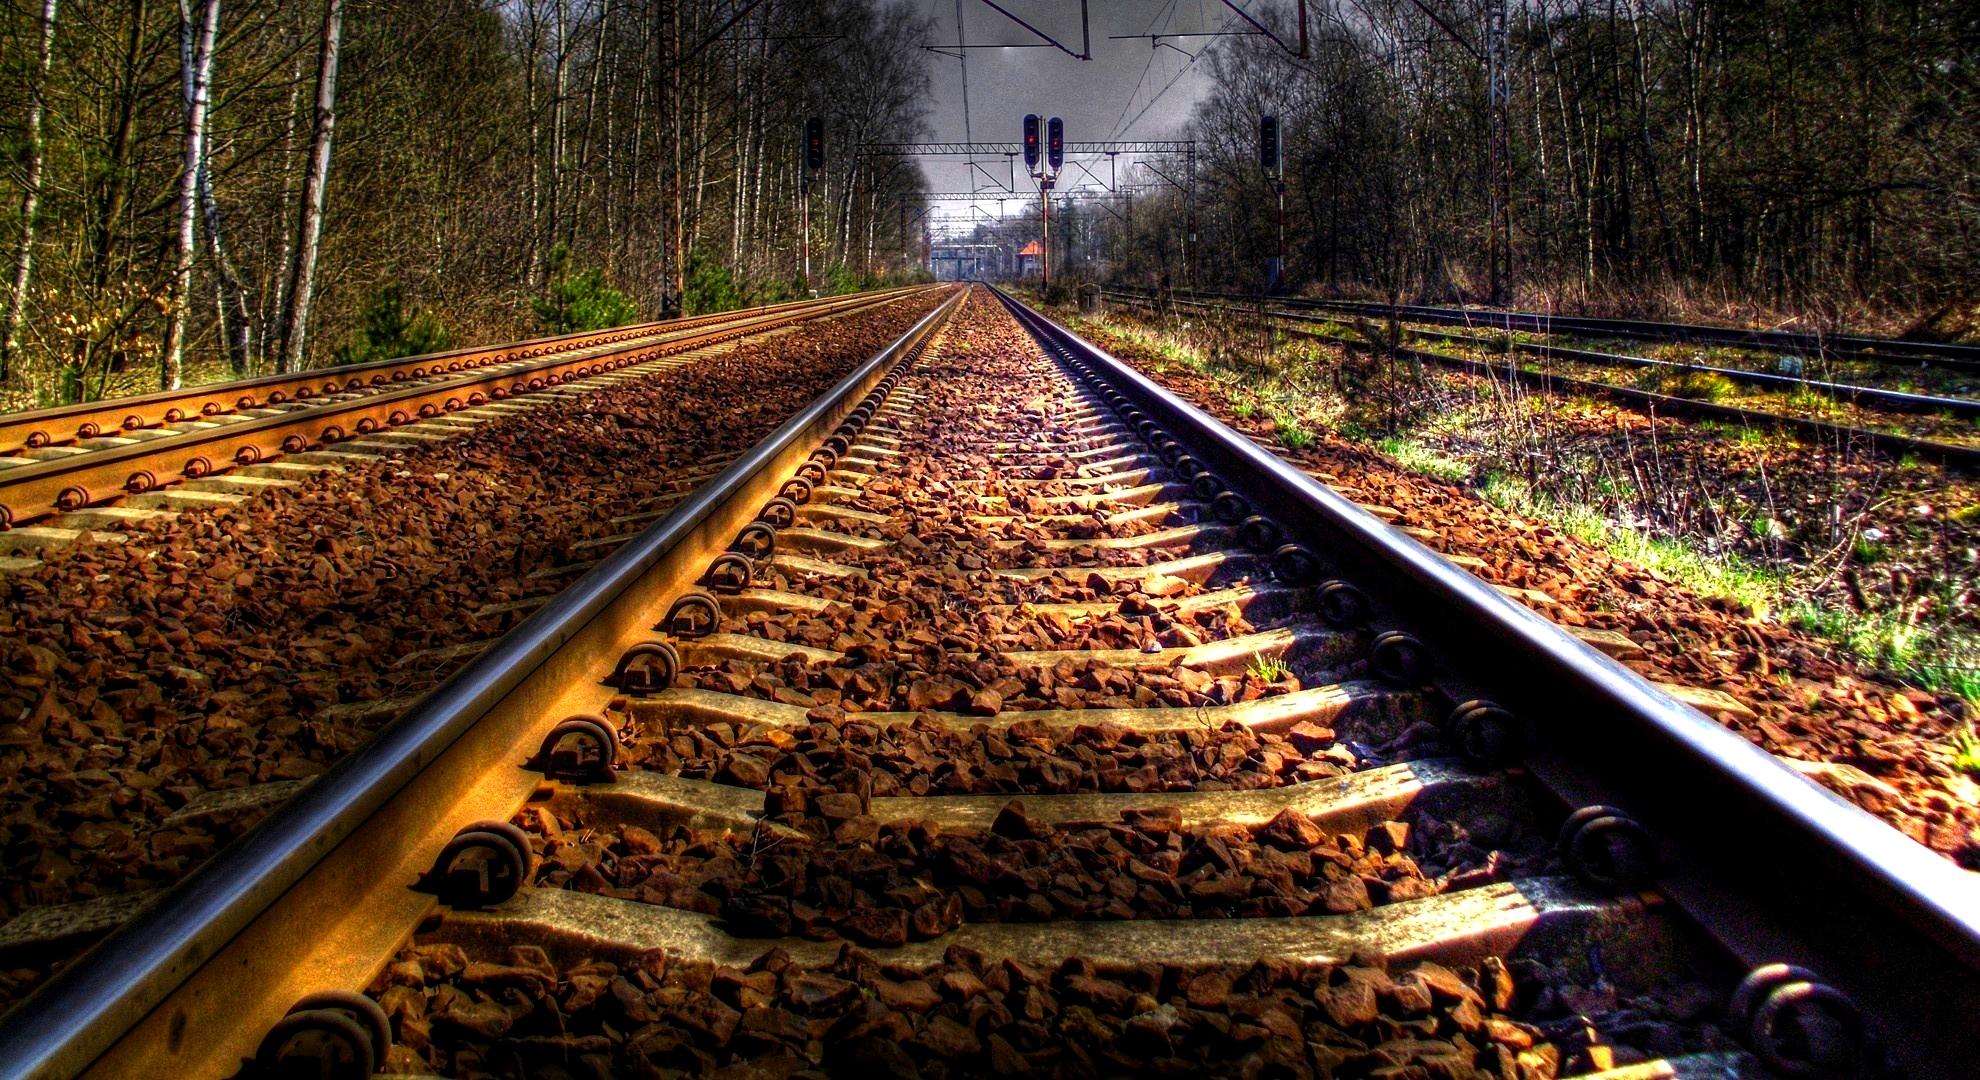
\includegraphics[scale=0.1]{TrainTrack}
    \caption{How projective space distorts parallelism present in Euclidean space}
    \label{fig:traintrack}
\end{figure}

Therefore the parallelism between the beams in Euclidean space is distorted in projective space. This phenomenon is referred to as perspective, where an object appears smaller the further away it is, and occurs as a result of reducing 3D information to a 2D image. According to this phenomenon a coordinate in 3D Euclidean space is mathematically related to a 2D coordinate in projective space through a scaling variable.

Homogeneous coordinates are simply Euclidean coordinates with this scaling variable added as an additional element in the coordinate vector. Homogeneous coordinates can be converted back to euclidean coordinates by scaling the vector by the scaling variable and then removing the scaling variable from the vector. In other words the homogeneous vector is multiplied by the inverse of the scaling variable and then the scaling variable is dropped from the vector.

Homogeneous coordinates aren't only useful for converting a coordinate from Euclidean space to projective space. They also allow translations and rotations to be applied to a coordinate vector using matrix multiplication. %As such homogeneous coordinates are used in the relation between world and sensor coordinates.

\section{Camera optics}
For an image of an object to be in focus the light incident upon each light sensor should originate from one point on the object's surface. However light is reflected by objects in many directions and so a means of focusing the light is required. This is accomplished through using lenses and an aperture. Throughout this project thin lenses are assumed. A thin lens is one in which its thickness is negligible in comparison with its focal length or radius of curvature \cite{sutton2009image}. Additionally the paraxial approximation is assumed which states that light rays passing through the lens do so with a small angle to the lens's optical axis and pass through the lens close to the optical axis. This leads to the small angle approximation.
\begin{equation}
  \sin(\theta) \approx \tan(\theta) \approx \theta
\end{equation}

Lenses are usually disk shaped pieces of glass with two convex surfaces. The convex surfaces are designed to bend light towards the optical axis with the degree of bending increasing with the distance from the light to optical axis at the lens mid plane. Thus diffuse light emanating from a point M $[x,y,z]^T$ on an object will pass through the lens and the light rays will converge at a point called the ideal image point M' $[x',y',z']^T$. Thereafter the light rays diverge again to points M'' $[x'', y'', z'']^T$ as shown in Figure \ref{fig:optics}. If the sensor plane is coincident with the ideal image points of the light rays the image that forms on the sensor is inverted due to the way the lens bends the light. As a result an inverted coordinate system is used for the sensor plane.

\begin{figure}[h]
    \centering
    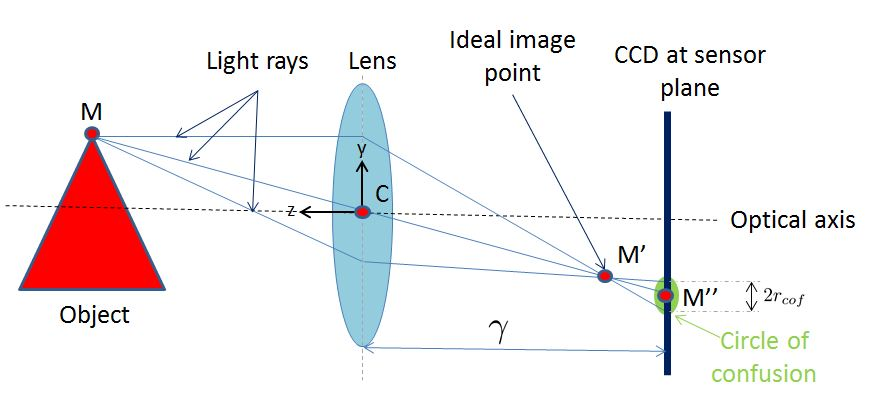
\includegraphics[scale=0.6]{Optics}
    \caption{Illustration of how light rays are manipulated by the lens}
    \label{fig:optics}
\end{figure}

% Due to the way the lens bends the light rays the image formed if the sensor plane is coincident with the resulting in an inverted image M'' (x'',y'',z'') if the sensor plane is behind the ideal image point. Since this is the most common camera configuration an inverted coordinate system is used for the sensor plane.

The thin lens equation can be stated as
\begin{equation}
\frac{1}{|CM|} + \frac{1}{CM'} = \frac{1}{\mean{f}}
\end{equation}
where $\mean{f}$ is the focal length; an inherent property of the lens. Additionally through similarity of triangles we have
\begin{align}
\frac{y}{CM} = \frac{-y'}{CM'}\\
\frac{x}{CM} = \frac{-x'}{CM'}\\
\frac{z}{CM} = \frac{-z'}{CM'}.
\end{align}
Combining these a series of equations for the ideal image point can be obtained.
\begin{align}
\label{eq:optics y'2y}
\begin{split}
x'&=\frac{-\mean{f} x}{z - \mean{f}} \\
y'&=\frac{-\mean{f} y}{z - \mean{f}} \\
z'&=\frac{-\mean{f} z}{z - \mean{f}}
\end{split}
\end{align}

\subsection{Circle of confusion}
It is impossible to align the sensor plane perfectly with the ideal image points and so the divergence of the light rays after the ideal image point causes the light rays to illuminate a circular area on the sensor plane. This blurred region is known as the circle of confusion. If this circular area is larger than the area spanned by an element of the sensor then this will result in blurring in the image as the light spills over multiple sensors. This blur could be eliminated by having the sensor plane the same distance from the lens as the the ideal image point but different points on the object will have different ideal image points.

The light rays that make up the outer perimeter of the circle of confusion are the rays that pass through the lens on the outer edges. Using these rays it is possible to determine the radius of the circle of confusion. Taking $r$ to be the radius of the lens these outer light rays pass through the midplane of the lens along the perimeter of a circle described by $[r \cos \beta, r \sin \beta, 0]^T$ where $0 \leq \beta \leq 2\pi$. Here $\beta$ is the angle subtended by the radius and the x axis that lies in plane with the lens. Using trigonometry the x and y components of these light rays can be related as
\begin{align}
  \frac{x' - r \cos \beta}{z'} &= \frac{x' - x''}{\gamma + z'} \\
  \frac{y' - r \sin \beta}{z'} &= \frac{y' - y''}{\gamma + z'} 
\end{align}
The distance between the midplane of the lens and the sensor plane is given by $\gamma$. Using these and Equation \ref{eq:optics y'2y} an expression for the perimeter of the circle of confusion can be found.
\begin{equation}
\label{eq:cof}
  \begin{bmatrix}
  x'' \\
  y'' \\
  z''
  \end{bmatrix} =
  \begin{bmatrix}
  r \cos \beta + r \cos \beta \left( 1 + \frac{\gamma \left( \mean{f} - z \right)}{\mean{f} z} \right) \\
  r \sin \beta + r \sin \beta \left( 1 + \frac{\gamma \left( \mean{f} - z \right)}{\mean{f} z} \right) \\
  0
  \end{bmatrix} +
  \begin{bmatrix}
  -\frac{\gamma x}{z} \\
  -\frac{\gamma y}{z} \\
  - \gamma
  \end{bmatrix}
\end{equation}
The radius of the circle of confusion can be determine by taking the difference in the y components of $y''$ for $\beta=90 ^{\circ} $ and $\beta=270 ^{\circ}$.

\begin{align}
  2 r_{cof} &= \left[r \sin 90 ^{\circ} \left( 2 + \frac{\gamma \left( \mean{f} - z \right)}{\mean{f} z} \right) \right] - \left[r \sin 270 ^{\circ} \left( 2 + \frac{\gamma \left( \mean{f} - z \right)}{\mean{f} z} \right) \right] \\
  r_{cof}&=r \left( 1 + \frac{\gamma \left( \mean{f} - z \right)}{\mean{f}z} \right)
\end{align}

Another way that the blur can be improved is by using an aperture. An aperture is at a basic level an opaque diaphragm with a hole in it which serves to reduce the amount of light that is incident upon the sensor. Thus by blocking off the light that passed through the outer edges of the lens the aperture reduces the size of the circle of confusion by effectively reducing the radius of the lens. The aperture can be place in front or behind the lens. 

\subsection{Depth of field}
Depth of field is defined as the distance ahead and behind the object that is in focus. For a particular camera system the ideal image point of an object will fall upon the sensor plane if the object is at an ideal focal length from the lens. If the object is any closer or further from the lens it will cause a circle of confusion on the sensor plane as opposed to a point. If the circle of confusion is small enough it will not spill significant light over multiple sensors which will result in a clear image.% be interpreted as a point by the light sensor in which case it is clear in the image.

However if the circle of confusion is large enough it will cause blurring in the image. The largest circle of confusion which still results in a sharp image is referred to as the acceptable circle of confusion \cite{sutton2009image}. Thus the depth of field can be considered as the distance along the z-axis ahead or behind the ideal focus length which results in an acceptable circle of confusion.

The largest degree of freedom for a specific camera system occurs when the object is at the hyperfocal length, $H$, from the camera. The hyperfocal length is defined as the closest an object can be to the camera such that the depth of field extends to infinity behind the object. In this situation the depth of field starts at a distance of $\frac{H}{2}$. The hyperfocal length can be approximated as
\begin{equation}
  H \simeq \frac{\mean{f}^2}{2 N r_{cof}}
  \label{eq:hyperfocal}
\end{equation}
Here $N$ is given by $\frac{\mean{f}}{D_p}$, where $D_p$ is the diameter of the entrance pupil for the camera system. Letting $s$ be the distance from the camera to the object such that the camera is ideally focused at a distance $s$. The distance from the camera to the near limit of the depth of field, $D_N$, and the distance from the camera to the far limit of the depth of field, $D_F$, can be approximated.
\begin{align}
  D_N \simeq \frac{Hs}{H+s} \\
  D_F \simeq \frac{Hs}{H-s}
\end{align}
These approximations assume that the object distance is large compared to the lens focal length. The depth of field can then be determined.
\begin{equation}
  DOF = D_F - D_N = \frac{2 H s^2}{H^2 - s^2}
  \label{eq:DOF}
\end{equation}
Combining Equation \ref{eq:hyperfocal} and \ref{eq:DOF} 
\begin{equation}
  DOF = \frac{4 N r_{cof} \mean{f}^2 s^2}{\mean{f}^4 - 4 N^2 r_{cof}^2 s^2}.
\end{equation}
Thus it is clear that the depth of field can be controlled by altering the focal length of the lens. This can be done by either changing the size of the aperture $D_p$ or by changing the distance between the camera and the object.

\subsection{Field of view}
\todo{viewing frustum}
The field of view is the extent of the world that the camera is capable of capturing in an image. It is quantified as the largest angle that a light ray, that is incident upon the sensor, makes with the optical axis. This angle is referred to as the angle-of-view.

Using the pinhole camera model with a distance of $L$ \todo{need to illustrate these dimensions in an image} between the sensor and the lens and taking the lens height to be $d$ a relation for the angle-of-view, $\alpha$, can be derived using trigonometry.
\begin{align}
  \tan \left( \frac{\alpha}{2} \right) &= \frac{d}{2 L} \\
  \alpha &= 2 \arctan \left( \frac{d}{2L} \right)
\end{align}

However for the best picture quality the distance between the sensor and the lens should be equal to the focal length $f$.
\begin{equation}
  \alpha = 2 \arctan \left( \frac{d}{2f} \right)
\end{equation}

% \subsection{Transformation to image plane}
% The relation between an object point and the projection of the object point onto the sensor can be derived from Equation \ref{eq:cof} by eliminating the circle of confusion component. Additionally when the camera system is set up properly $z'$ will be equal to $\gamma$ so that the sensor plane is approximately coincident with the ideal image points. 
% \begin{equation}
% \label{eq:w2i}
%   \begin{bmatrix}
%   x'' \\
%   y'' \\
%   z''
%   \end{bmatrix} = 
%   \begin{bmatrix}
%   -\frac{\gamma}{z} & 0 & 0 \\
%   0 & -\frac{\gamma}{z} & 0 \\
%   0 & 0 & -\gamma
%   \end{bmatrix}
%   \begin{bmatrix}
%   x \\
%   y \\
%   1
%   \end{bmatrix}
% \end{equation}
% This equation presents two issues. Firstly the dependence of the sensor positions on $z$. Secondly all the terms in the equation have metric units whereas the image coordinate system has dimensions measured in pixels. These issues are fixed by using a homogeneous from of Equation \ref{eq:w2i}.
% \begin{equation}
% \label{eq:w2ih}
%   \alpha \begin{bmatrix}
%   -x'' \\
%   -y'' \\
%   1
%   \end{bmatrix} =
%   \begin{bmatrix}
%   \gamma & 0 & 0 & 0 \\
%   0 & \gamma & 0 & 0 \\
%   0 & 0 & 1 & 0
%   \end{bmatrix}
%   \begin{bmatrix}
%   x \\
%   y \\
%   z \\
%   1
%   \end{bmatrix}
% \end{equation}
% Here $\alpha$ is a scale factor which allows for the conversion from metric units for the world coordinate system to pixels used in the sensor coordinate system. This equation is referred to as perspective projection \cite{sutton2009image}.

\subsection{Front image plane model}
A new imaging model that is often preferred for computer vision applications can be obtained by translating the sensor plane a distance of $2\gamma$ along the optical axis. In this case the sensor plane is in front of the lens. Treating the sensor coordinates $M''$ of an object as the intersection of the light ray with the sensor plane; Equation \ref{eq:w2ih} remains valid for this configuration.

This imaging model is advantageous in that the sensor plane coordinates are no longer inverted. This means that the scene being imaged is also not inverted.

\todo{the perspective projection does not involve negative values now}

% \begin{itemize}
%   \item intro
%   \item circle of confusion
%   \item M to M''
%   \item aperture
%   \item DOF
%   \item angle of view
%   \item pinhole inversion
% \end{itemize}

% The surfaces are convex such that diffuse light emanating from a point on an object that passes through the lens will converge and intersect at a point called the ideal imaging point. After the ideal imaging point the light rays begin to diverge again. Once this divergence occurs the image becomes inverted. The lens is placed in front of the sensor plane in an attempt to focus the light from each part of the object onto a single light sensor.

% Lenses are usually disk shaped pieces of glass with two convex surfaces. The surfaces are convex such that diffuse light emanating from a point on an object that passes through the lens will converge and intersect at a point called the ideal imaging point. After the ideal imaging point the light rays begin to diverge again. Once this divergence occurs the image becomes inverted. The lens is placed in front of the sensor plane in an attempt to focus the light from each part of the object onto a single light sensor.

% This is illustrated in figure \todo{figure}.

%  which refract light that passes through them to bring the light closer to the usually shaped such that they have convex surfaces that are shaped in such a way that light passing through the lens is refracted towards the optical axis such that  

\section{Coordinate systems}
There are four coordinate systems involved in converting a coordinate on an object in the real world to a corresponding coordinate in an image of the object. 

\begin{figure}[H]
    \centering
    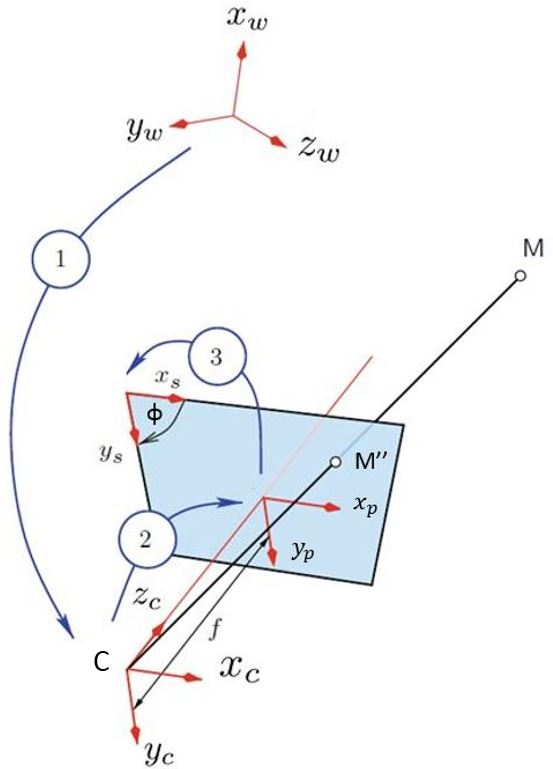
\includegraphics[scale=0.5]{CoordinateSystems}
    \caption{The conversion between coordinate systems that occurs when an image is taken \cite{sutton2009image}}
    \label{fig:coordsys}
\end{figure}

These coordinate systems are the world coordinate system represented by subscript $w$, the camera coordinate system represented by subscript $c$, the image plane coordinate system represented by subscript $p$ and the sensor coordinate system represented by subscript $s$. This section presents these four coordinate systems and the mathematical relations used to convert coordinates between them.

\subsection{World to camera coordinate system}
The world coordinate system is simply the coordinate system that is used to classify the position of objects in the real world,$(x_w, y_w, z_w)$. Its orientation and origin are arbitrary and it is usually classified according to the calibration plate used. \todo{Can i say calibration plate without defining it yet} The camera coordinate system is fixed according to the cameras position and orientation where the z-axis is the optical axis of the camera. Camera coordinates are represented as $(x_c, y_c, z_c)$.

Converting from the world coordinate system to the camera coordinate system involves rigid transformations of translation $T$ and rotation $R$. 
\begin{equation}
\label{eq: world2camera}
  \bm{X}_c = 
  \begin{bmatrix}
  x_c \\
  y_c \\
  z_c \\
  1
  \end{bmatrix}
  =
  \begin{bmatrix}
  r_{11} & r_{12} & r_{13} & t_1 \\
  r_{21} & r_{22} & r_{23} & t_2 \\
  r_{31} & r_{32} & r_{33} & t_3 \\
  0 & 0 & 0 & 1
  \end{bmatrix}
  \begin{bmatrix}
  x_w \\
  y_w \\
  z_w \\
  1
  \end{bmatrix} = 
  \begin{bmatrix}
  \bm{R} & \bm{T} \\
  \bm{0} & 1
  \end{bmatrix} \bm{X}_w.
\end{equation}
\todo{change T and R to lowercase}
The parameters in $\bm{R}$ and $\bm{T}$ are referred to as extrinsic parameters since they are not dependent on the camera system's hardware but rather the camera's position and orientation in the world coordinate system.

% Scaling of dimensions between the two coordinate systems also needs to be taken into account. The parameters in $\bm{R}$ and $\bm{T}$ are referred to as extrinsic parameters since they are not dependent on the camera system's hardware but rather the camera's position and orientation in the world coordinate system.

\subsection{Camera and image plane coordinates}
The image plane coordinate system is an orthogonal coordinate system that has its x-y plane coincident with the plane of the CCD sensor array. Its z-axis is also coincident with the z-axis of the camera coordinate system. Although this coordinate system has three dimensions its coordinates all lie on the x-y plane and so it can be treated as a 2D coordinate system. \todo{improve this}

Conversion of a coordinate from the camera coordinate system to the image plane coordinate system involves perspective projection. This relation can be derived from Equation \ref{eq:cof} by eliminating the circle of confusion component and substituting the appropriate dimensions. Additionally when the camera system is set up properly $z'$ will be equal to $\gamma$ so that the sensor plane is approximately coincident with the ideal image points. %Thus $z_c'$ will be approximately equal to $\gamma$ as well.
\begin{equation}
\label{eq:w2i}
  \begin{bmatrix}
  x_c' \\
  y_c' \\
  z_c'
  \end{bmatrix} = 
  \begin{bmatrix}
  \frac{\gamma}{z_c} & 0 & 0 \\
  0 & \frac{\gamma}{z_c} & 0 \\
  0 & 0 & \gamma
  \end{bmatrix}
  \begin{bmatrix}
  x_c \\
  y_c \\
  1
  \end{bmatrix}
\end{equation}

Here $(x_c', y_c', z_c')$ are the camera coordinates projected onto the image plane but stipulated within the camera coordinate system. Note that the since the front image plane model is used the dimensions are now non-negative. The issue with this equation is the dependence on $z_c$ in the matrix. This is fixed by using a homogeneous form of Equation \ref{eq:w2i}.

\begin{equation}
\label{eq:w2ih}
  \alpha \begin{bmatrix}
  x_c' \\
  y_c' \\
  z_c' \\
  1
  \end{bmatrix} =
  \begin{bmatrix}
  \gamma & 0 & 0 & 0 \\
  0 & \gamma & 0 & 0 \\
  0 & 0 & \gamma & 0 \\
  0 & 0 & 1 & 0
  \end{bmatrix}
  \begin{bmatrix}
  x_c \\
  y_c \\
  z_c \\
  1
  \end{bmatrix}
\end{equation}

This equation is referred to as perspective projection \cite{sutton2009image}. Here $\alpha$ is the scaling variable of the homogeneous coordinates. It is divided out of the homogeneous coordinate vector so that the coordinate is correctly scaled on the image plane. \todo{make sure this is correct}%so that this vector can be easy converted back to a 3D vector in Euclidean space. 
The value of $\alpha$ is equal to $z_c$ and $z_c'$ is equal to $\gamma$ such that this coordinate lies on the image plane.

Converting this projected coordinate to the image plane coordinate system is achieved by dropping the z dimension to obtain
\begin{equation}
\label{eq:c2i}
  \bm{X}_p = \begin{bmatrix}
  x_p \\
  y_p \\
  1
  \end{bmatrix}
  = \begin{bmatrix} 
  1 & 0 & 0 & 0 \\
  0 & 1 & 0 & 0 \\
  0 & 0 & 0 & 1
  \end{bmatrix}
  \begin{bmatrix}
  x_c' \\
  y_c' \\
  z_c' \\
  1
  \end{bmatrix} = \begin{bmatrix}
  \gamma & 0 & 0 & 0 \\
  0 & \gamma & 0 & 0 \\
  0 & 0 & 1 & 0
  \end{bmatrix}
  \begin{bmatrix}
  x_c \\
  y_c \\
  z_c \\
  1
  \end{bmatrix}
\end{equation}


% Here $\alpha$ is a scale factor which allows for the conversion from metric units for the world coordinate system to pixels used in the image plane coordinate system. This equation is referred to as perspective projection \cite{sutton2009image}.

\subsection{Image plane and sensor coordinates}
At this point the locations of where the light rays originating from the object will intersect the image plane are known. Now it is necessary to mathematically represent how the sensor would interpret these light rays incident upon the sensor into the form of a matrix of pixels. In order to do this a relation between the position of a point within a coordinate system and the pixel within an image is necessary. Additionally the sensor array is not guaranteed to the orthogonal and so a skewed coordinate system must be taken into account.

The transformation from the image plane coordinate system to a temporary skewed coordinate system with an angle of $\phi$ between the two axes can be represented by
\begin{equation}
\label{eq:plane2skew}
  \begin{bmatrix}
  x_{temp} \\
  y_{temp} 
  \end{bmatrix} =
  \begin{bmatrix}
  1 & -\cot \phi \\
  0 & \frac{1}{\sin \phi}
  \end{bmatrix}
  \begin{bmatrix}
  x_p\\
  y_p
  \end{bmatrix}.
\end{equation}
It is assumed that the two principle directions in the sensor coordinate system have different scale factors, $S_x$ and $S_y$, which have units of pixels per unit length. Additionally the sensor coordinate system has its origin at one of the corners of the image plane such that all coordinates that fall on the image plane are positive. This is because these coordinates represent positions within a matrix. As such the coordinates need to be translated by $\hat c_x$ and $\hat c_y$ to account for the origin of the sensor coordinate system. 

Note that these translations are given in terms of the image plane coordinate system. Applying these to the coordinates calculated in equation \ref{eq:plane2skew} results in the sensor coordinates below.

% Applying these to the coordinates calculated in equation \ref{eq:plane2skew} and accounting for the translations $\hat c_x$ and $\hat c_y$ to convert to the origin of the sensor coordinate system results in the sensor coordinates below.
\begin{equation}
  \begin{bmatrix}
  x_s \\
  y_s
  \end{bmatrix} = 
  \begin{bmatrix}
  S_x & 0\\
  0 & S_y
  \end{bmatrix}
  \begin{bmatrix}
  x_{temp}\\
  y_{temp}
  \end{bmatrix} -
  \begin{bmatrix}
  S_x \hat c_x - S_x \hat c_y \cot \phi \\
  \frac{S_y \hat c_y}{\sin \phi}
  \end{bmatrix}=
  \begin{bmatrix}
  S_x & -S_x \cot \phi \\
  0 & \frac{S_y}{\sin \phi}
  \end{bmatrix}
  \begin{bmatrix}
  x_p \\
  y_p
  \end{bmatrix} -
  \begin{bmatrix}
  S_x \hat c_x - S_x \hat c_y \cot \phi \\
  \frac{S_y \hat c_y}{\sin \phi}
  \end{bmatrix}
\end{equation}

This can be rewritten in homogeneous form so that it is consistent with equation \ref{eq:c2i}.
\begin{equation}
\label{eq: image2sensor}
  \bm{X}_s = 
  \begin{bmatrix}
  x_s \\
  y_s \\
  1
  \end{bmatrix} =
  \begin{bmatrix}
  S_x & -S_x \cot \phi & -S_x \left( \hat c_x - \hat c_y \cot \phi \right) \\
  0 & \frac{S_y}{\sin \phi} & -\frac{S_y \hat c_y}{\sin \phi} \\
  0 & 0 & 1
  \end{bmatrix}
  \begin{bmatrix}
  x_p \\
  y_p \\
  1
  \end{bmatrix} =
  \bm{A} \bm{X}_p
\end{equation}
\todo{talk about these parameters being intrinsic and combine them better}

\subsection{World to sensor coordinates}
The conversions between coordinate systems described in Equations \ref{eq: world2camera}, \ref{eq:c2i} and \ref{eq: image2sensor} can be combined into one conversion from the world coordinate system to the sensor coordinate system.
\begin{equation}
  \bm{X}_s = \alpha
  \begin{bmatrix}
  x_s \\
  y_s \\
  1
  \end{bmatrix} =
  \begin{bmatrix}
  S_x & -S_x \cot \phi & -S_x \left( \hat c_x - \hat c_y \cot \phi \right) \\
  0 & \frac{S_y}{\sin \phi} & -\frac{S_y \hat c_y}{\sin \phi} \\
  0 & 0 & 1
  \end{bmatrix}
  \begin{bmatrix}
  \gamma & 0 & 0 & 0 \\
  0 & \gamma & 0 & 0 \\
  0 & 0 & 1 & 0
  \end{bmatrix}
  \begin{bmatrix}
  r_{11} & r_{12} & r_{13} & t_1 \\
  r_{21} & r_{22} & r_{23} & t_2 \\
  r_{31} & r_{32} & r_{33} & t_3 \\
  0 & 0 & 0 & 1
  \end{bmatrix}
  \begin{bmatrix}
  x_w \\
  y_w \\
  z_w \\
  1
  \end{bmatrix}
\end{equation}

This can be simplified by combining the first two matrices.
\begin{align}
  \bm{X}_s = \alpha
  \begin{bmatrix}
  x_s \\
  y_s \\
  1
  \end{bmatrix} =
  \begin{bmatrix}
  \gamma S_x & -\gamma S_x \cot \phi & -S_x \left( \hat c_x - \hat c_y \cot \phi \right) & 0\\
  0 & \frac{\gamma S_y}{\sin \phi} & -\frac{S_y \hat c_y}{\sin \phi} & 0\\
  0 & 0 & 1 & 0
  \end{bmatrix}
  \begin{bmatrix}
  r_{11} & r_{12} & r_{13} & t_1 \\
  r_{21} & r_{22} & r_{23} & t_2 \\
  r_{31} & r_{32} & r_{33} & t_3 \\
  0 & 0 & 0 & 1
  \end{bmatrix}
  \begin{bmatrix}
  x_w \\
  y_w \\
  z_w \\
  1
  \end{bmatrix}
  \label{eq:world 2 sensor cumbersome}
\end{align}

Replacing the elements of the first matrix in equation \ref{eq:world 2 sensor cumbersome} with single variables for the purposes of simplicity the equation can be rewritten as

\begin{align}
  \alpha
  \begin{bmatrix}
  x_s \\
  y_s \\
  1
  \end{bmatrix} &=
  \begin{bmatrix}
  f_x & f_s & c_x & 0\\
  0 & f_y & c_y & 0\\
  0 & 0 & 1 & 0
  \end{bmatrix}
  \begin{bmatrix}
  r_{11} & r_{12} & r_{13} & t_1 \\
  r_{21} & r_{22} & r_{23} & t_2 \\
  r_{31} & r_{32} & r_{33} & t_3 \\
  0 & 0 & 0 & 1
  \end{bmatrix}
  \begin{bmatrix}
  x_w \\
  y_w \\
  z_w \\
  1
  \end{bmatrix} \\
  &= \bm{K} \bm{V} \bm{X}_w.
  \label{eq:world 2 sensor}
\end{align}
Here the parameters relating the world coordinate system to the sensor coordinate system are separated into two matrices. The first matrix $\bm{K}$ contains the intrinsic parameters which are fixed for a specific camera since they are dependent on the hardware that makes up the camera system. The second matrix $\bm{V}$ contains the extrinsic parameters that explain how the camera is orientated with respect to the calibration plate which defines the world coordinate system. Thus extrinsic parameters change when the camera's position and orientation relative to the world coordinate system changes.



% \subsection{Homogeneous coordinates}
% It is common knowledge that any object's shape can be fully defined using distances and angles in 3D Euclidean space. However when an image is taken of this object these distances and angles become distorted. For example railway tracks consist of two beams that remain parallel to one another at a set distance apart in Euclidean space but in an image of the railway track (projective space) these beams appear to get closer and closer to one another as seen in figure \ref{fig:traintrack}. Therefore the parallelism between the beams in Euclidean geometry is distorted in projective geometry. This occurs as a result of reducing 3D information to a 2D image. \todo{add image}

% \begin{figure}[H]
%     \centering
%     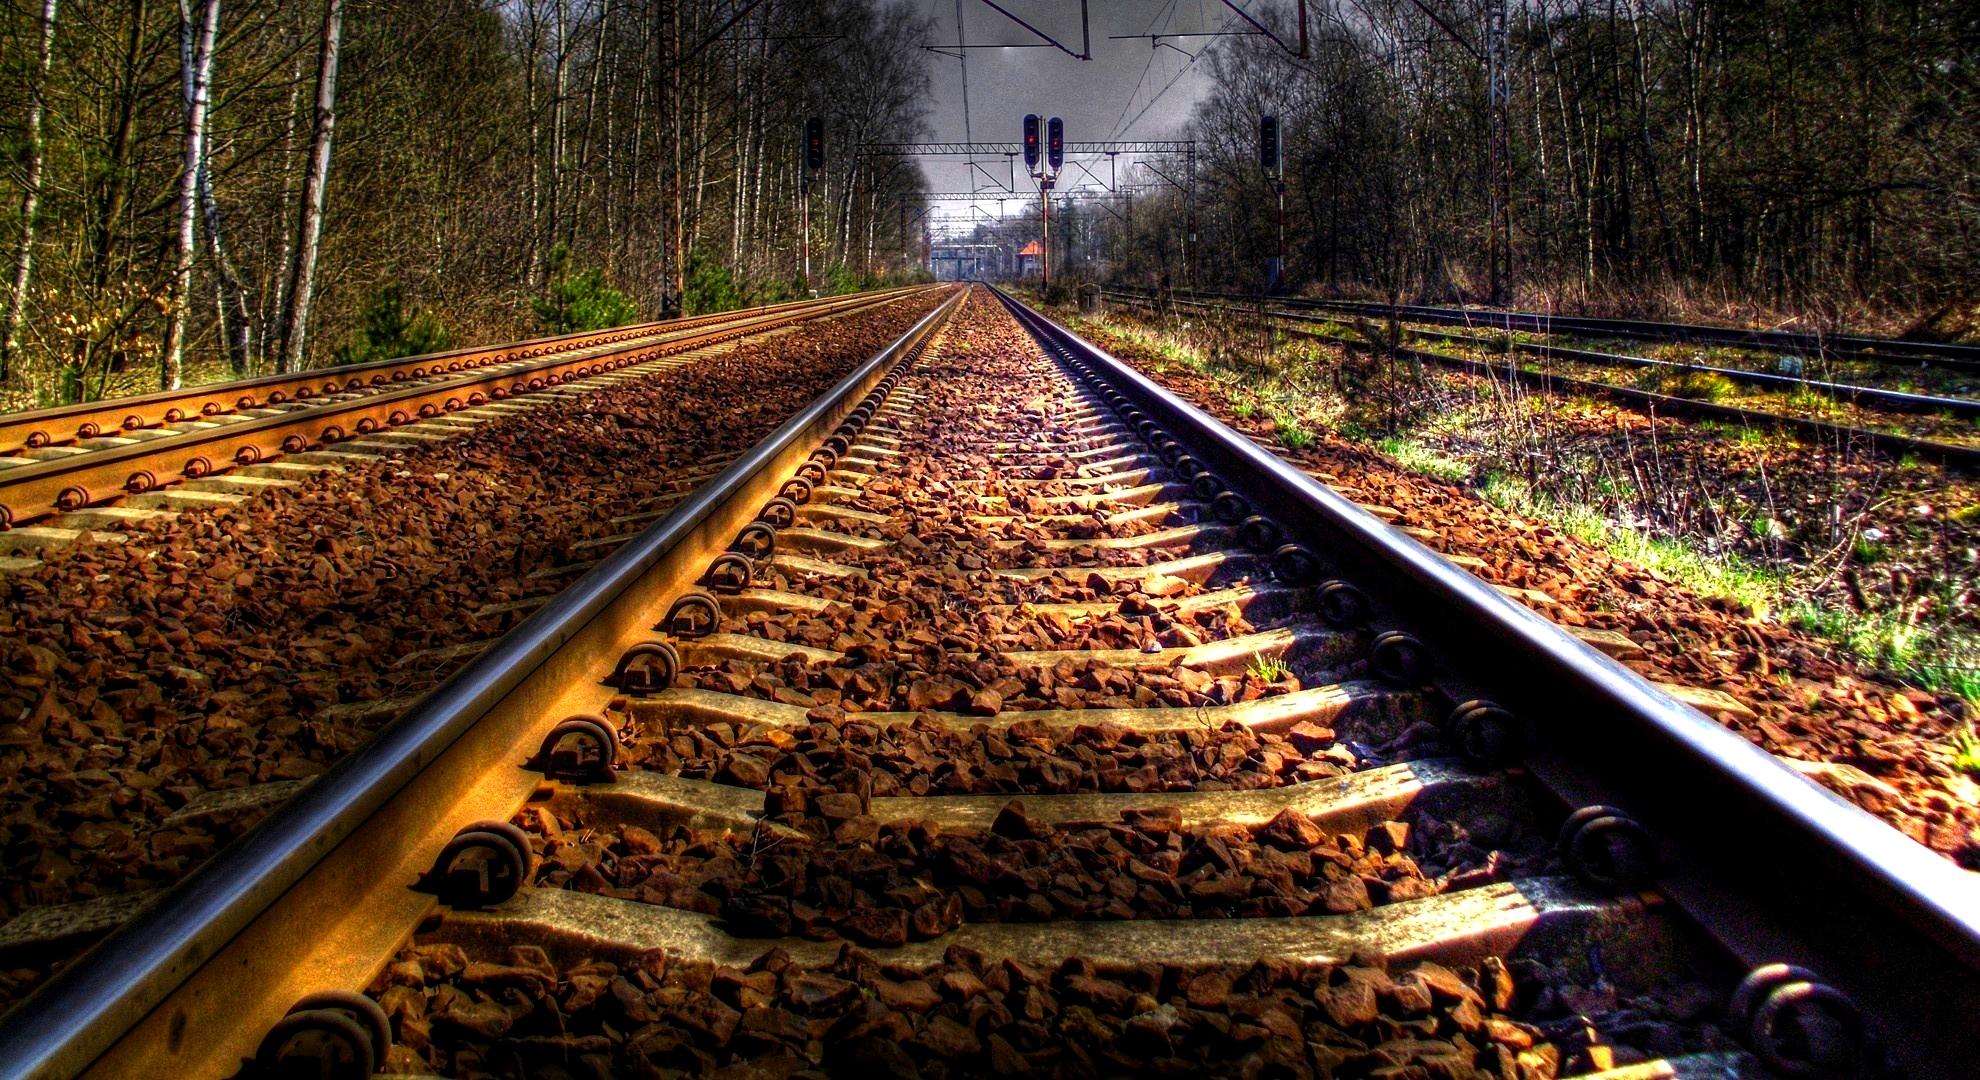
\includegraphics[scale=0.1]{TrainTrack}
%     \caption{How projective space distorts parallelism present in Euclidean space}
%     \label{fig:traintrack}
% \end{figure}

% Therefore the parallelism between the beams in Euclidean space is distorted in projective space. This phenomenon is referred to as perspective, where an object appears smaller the further away it is, and occurs as a result of reducing 3D information to a 2D image. According to this phenomenon a coordinate in 3D Euclidean space is mathematically related to a 2D coordinate in projective space through a scaling variable.

% Homogeneous coordinates are simply Euclidean coordinates with this scaling variable added as an additional element in the coordinate vector. Homogeneous coordinates can be converted back to euclidean coordinates by scaling the vector by the scaling variable and then removing the scaling variable from the vector. In other words the homogeneous vector is multiplied by the inverse of the scaling variable and then the scaling variable is dropped from the vector.

% Homogeneous coordinates aren't only useful for converting a coordinate from Euclidean space to projective space. They also allow translations and rotations to be applied to a coordinate vector using matrix multiplication. As such homogeneous coordinates are used in the relation between world and sensor coordinates.

% homogeneous coordinates needed for scaling of coordinates to create perspective geometry and for applying transformation and rotation using matrix multiplication

% Homogeneous coordinates are used to define how 3D information in the real world is converted to a 2D image. 

% explain scaling and how its allows conversion between euclidean and projective. Then explain how its makes transformation and rotations easier to apply.

% \section{Coordinate systems(old)}
% \label{sec:coord sys}
% Images are only capable of storing two dimensional information whereas we live in a three dimensional world. Thus cameras convert three dimensional information from the world coordinate system into two dimensional information in the sensor coordinate system when a picture is taken as shown in Figure \ref{fig:coordsys}. The mathematical relationship between these two coordinate systems is discussed here.

% % \begin{figure}[H]
% %     \centering
% %     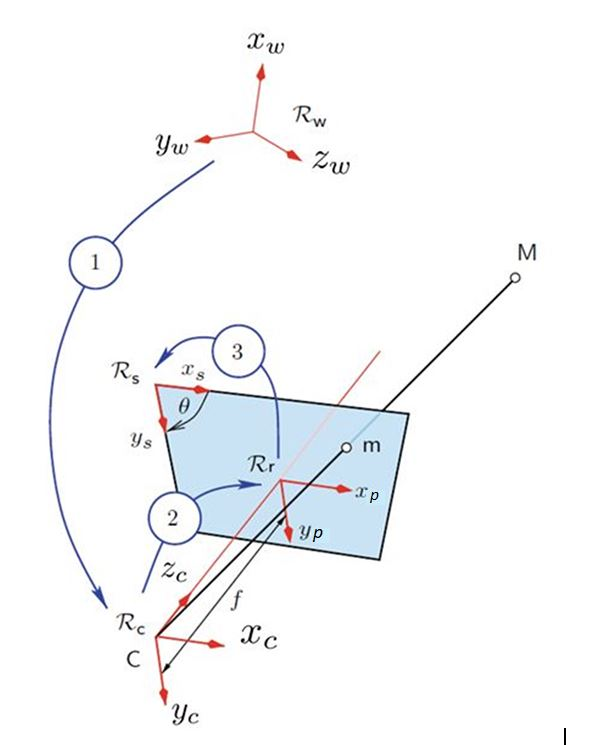
\includegraphics[scale=0.5]{CoordinateSystems2}
% %     \caption{The conversion between coordinate systems that occurs when an image is taken \cite{sutton2009image}}
% %     \label{fig:coordsys}
% % \end{figure}

% \todo{make sure the symbols are the same as used in the text and possibly rework this image (it is pretty original still)}
% % Throughout this project thin lenses are assumed. A thin lens is one in which its thickness is negligible in comparison with its focal length or radius of curvature. Additionally the paraxial approximation is assumed which states that light rays passing through the lens do so with a small angle to the lens's optical axis and pass through the lens close to the optical axis. This leads to the small angle approximation.
% % \begin{equation}
% %   \sin(\theta) \approx \tan(\theta) \approx \theta
% % \end{equation}
% \todo[inline]{describe how homogeneous coordinates allow n dim vectors to be manipulated in n+1 dim space}
% \subsection{Homogeneous coordinates}
% It is common knowledge that any object's shape can be fully defined using distances and angles in 3D Euclidean space. However when an image is taken of this object these distances and angles become distorted. For example railway tracks consist of two beams that remain parallel to one another at a set distance apart in Euclidean space but in an image of the railway track (projective space) these beams appear to get closer and closer to one another as seen in figure \ref{fig:traintrack}. Therefore the parallelism between the beams in Euclidean space is distorted in projective space. This occurs as a result of reducing 3D information to a 2D image. \todo{add image}

% \begin{figure}[H]
%     \centering
%     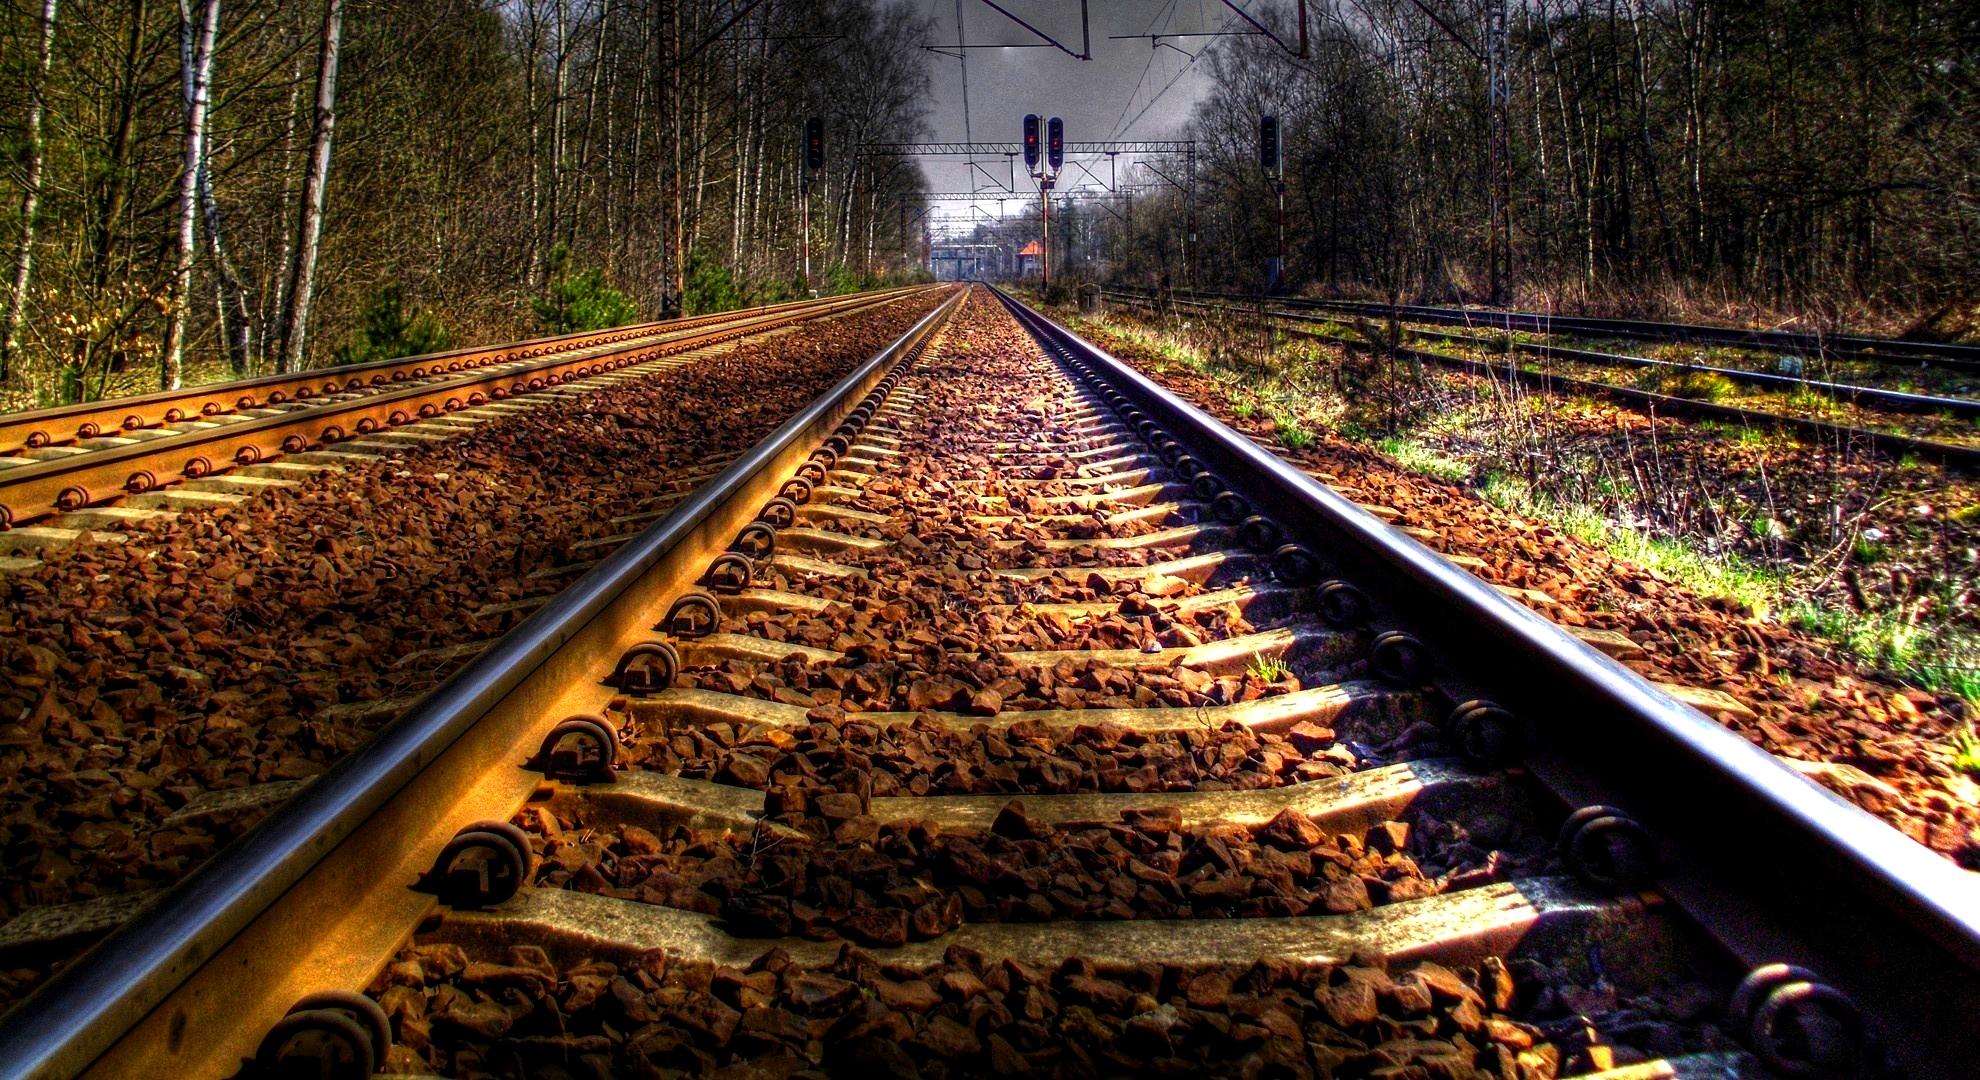
\includegraphics[scale=0.1]{TrainTrack}
%     \caption{How projective space distorts parallelism present in Euclidean space}
%     \label{fig:traintrack}
% \end{figure}

% Homogeneous coordinates make it possible to take a 3D coordinate in Euclidean space into a 4D coordinate in projective space. This is necessary since a transformation matrix for 3D coordinates that applies both rotation and translation has 4 columns and so can only be applied to a 4D coordinate. Conversion to homogeneous coordinates involves adding an additional coordinate $w$ to the coordinate vector and setting $w=1$. To convert back from homogeneous coordinates requires dividing the $x$, $y$ and $z$ coordinates by $w$ and then eliminating $w$.

% \todo{do a 2D example}
% % http://www.songho.ca/math/homogeneous/homogeneous.html
% % http://www.tomdalling.com/blog/modern-opengl/explaining-homogenous-coordinates-and-projective-geometry/
% \subsection{World to camera coordinate system}
% Converting from the world coordinate system to the camera coordinate system involves rigid transformations of translation $T$ and rotation $R$. The world coordinate system is simply the coordinate system that would be used to classify the position and orientation of objects in the real world. The world coordinate systems orientation and origin is somewhat arbitrary and it is usually classified according to the object to be imaged. 

% The camera coordinate system is as the name suggests fixed according to the cameras position and orientation. The camera coordinate system's z axis is the optical axis of the camera. The conversion between the two coordinate systems can be represented as
% \begin{equation}
%   \bm{X}_c = 
%   \begin{bmatrix}
%   x_c \\
%   y_c \\
%   z_c \\
%   1
%   \end{bmatrix}
%   =
%   \begin{bmatrix}
%   r_{11} & r_{12} & r_{13} & t_1 \\
%   r_{21} & r_{22} & r_{23} & t_2 \\
%   r_{31} & r_{32} & r_{33} & t_3 \\
%   0 & 0 & 0 & 1
%   \end{bmatrix}
%   \begin{bmatrix}
%   x_w \\
%   y_w \\
%   z_w \\
%   1
%   \end{bmatrix} = 
%   \begin{bmatrix}
%   \bm{R} & \bm{T} \\
%   \bm{0} & 1
%   \end{bmatrix} \bm{X}_w.
% \end{equation}
% \todo{change T and R to lowercase}
% Scaling of dimensions between the two coordinate systems also needs to be taken into account. The parameters in $\bm{R}$ and $\bm{T}$ are referred to as extrinsic parameters since they are not dependent on the camera system's hardware but rather the camera's position and orientation in the world coordinate system.

% \subsection{Camera and imaging plane coordinates}
% The 3D object defined in the camera coordinate system is converted to its projection on imaging plane. This conversion is from a 3D coordinate system to a 2D coordinate system as given below using homogeneous coordinates.
% \begin{equation}
% \label{eq:c2i}
%   \bm{X}_p = \alpha
%   \begin{bmatrix}
%   x_p \\
%   y_p \\
%   1
%   \end{bmatrix} 
%   = 
%   \begin{bmatrix}
%   \gamma & 0 & 0 & 0 \\
%   0 & \gamma & 0 & 0 \\
%   0 & 0 & 1 & 0
%   \end{bmatrix}
%   \begin{bmatrix}
%   x_c \\
%   y_c \\
%   z_c \\
%   1
%   \end{bmatrix}
% \end{equation}
% The variable $\alpha$ is an arbitrary scale factor.

% \subsection{Image plane and sensor coordinates}
% At this point the locations of where the light rays originating from the object will intersect the imaging plane are known. Now it is necessary to mathematically represent how the sensor would interpret these light rays incident upon the sensor into the form of pixels. In order to do this a relation between the position of a point within a coordinate system and the pixel within an image is necessary. Additionally the sensor array is not guaranteed to the orthogonal and so a skewed coordinate system must be taken into account.

% The transformation from the image plane coordinate system to a temporary skewed coordinate system with an angle of $\phi$ between the two axes can be represented by
% \begin{equation}
% \label{eq:plane2skew}
%   \begin{bmatrix}
%   x_{temp} \\
%   y_{temp} 
%   \end{bmatrix} =
%   \begin{bmatrix}
%   1 & -\cot \phi \\
%   0 & \frac{1}{\sin \phi}
%   \end{bmatrix}
%   \begin{bmatrix}
%   x_p\\
%   y_p
%   \end{bmatrix}.
% \end{equation}
% It is assumed that the two principle directions in the sensor coordinate system have different scale factors, $S_x$ and $S_y$,which have units of pixels per unit length. Applying these to the coordinates calculated in equation \ref{eq:plane2skew} and accounting for the translations $\hat c_x$ and $\hat c_y$ to convert to the origin of the sensor coordinate system results in the sensor coordinates below.
% \begin{equation}
%   \begin{bmatrix}
%   x_s \\
%   y_s
%   \end{bmatrix} = 
%   \begin{bmatrix}
%   S_x & 0\\
%   0 & S_y
%   \end{bmatrix}
%   \begin{bmatrix}
%   x_{temp}\\
%   y_{temp}
%   \end{bmatrix} -
%   \begin{bmatrix}
%   S_x \hat c_x - S_x \hat c_y \cot \phi \\
%   \frac{S_y \hat c_y}{\sin \phi}
%   \end{bmatrix}=
%   \begin{bmatrix}
%   S_x & -S_x \cot \phi \\
%   0 & \frac{S_y}{\sin \phi}
%   \end{bmatrix}
%   \begin{bmatrix}
%   x_p \\
%   y_p
%   \end{bmatrix} -
%   \begin{bmatrix}
%   S_x \hat c_x - S_x \hat c_y \cot \phi \\
%   \frac{S_y \hat c_y}{\sin \phi}
%   \end{bmatrix}
% \end{equation}

% This can be rewritten in homogeneous form so that it is consistent with equation \ref{eq:c2i}.
% \begin{equation}
%   \bm{X}_s = 
%   \begin{bmatrix}
%   x_s \\
%   y_s \\
%   1
%   \end{bmatrix} =
%   \begin{bmatrix}
%   S_x & -S_x \cot \phi & -S_x \left( \hat c_x - \hat c_y \cot \phi \right) \\
%   0 & \frac{S_y}{\sin \phi} & -\frac{S_y \hat c_y}{\sin \phi} \\
%   0 & 0 & 1
%   \end{bmatrix}
%   \begin{bmatrix}
%   x_p \\
%   y_p \\
%   1
%   \end{bmatrix} =
%   \bm{A} \bm{X}_i
% \end{equation}
% \todo{talk about these parameters being intrinsic and combine them better}

% \subsection{World to sensor coordinates}
% The conversions between coordinate systems described in the previous sections can be combined into one conversion from the world coordinate system to the sensor coordinate system.
% \begin{equation}
%   \bm{X}_s = \alpha
%   \begin{bmatrix}
%   x_s \\
%   y_s \\
%   1
%   \end{bmatrix} =
%   \begin{bmatrix}
%   S_x & -S_x \cot \phi & -S_x \left( \hat c_x - \hat c_y \cot \phi \right) \\
%   0 & \frac{S_y}{\sin \phi} & -\frac{S_y \hat c_y}{\sin \phi} \\
%   0 & 0 & 1
%   \end{bmatrix}
%   \begin{bmatrix}
%   \gamma & 0 & 0 & 0 \\
%   0 & \gamma & 0 & 0 \\
%   0 & 0 & 1 & 0
%   \end{bmatrix}
%   \begin{bmatrix}
%   r_{11} & r_{12} & r_{13} & t_1 \\
%   r_{21} & r_{22} & r_{23} & t_2 \\
%   r_{31} & r_{32} & r_{33} & t_3 \\
%   0 & 0 & 0 & 1
%   \end{bmatrix}
%   \begin{bmatrix}
%   x_w \\
%   y_w \\
%   z_w \\
%   1
%   \end{bmatrix}
% \end{equation}

% This can be simplified by combining the first two matrices.
% \begin{align}
%   \bm{X}_s = \alpha
%   \begin{bmatrix}
%   x_s \\
%   y_s \\
%   1
%   \end{bmatrix} =
%   \begin{bmatrix}
%   \gamma S_x & -\gamma S_x \cot \phi & -S_x \left( \hat c_x - \hat c_y \cot \phi \right) & 0\\
%   0 & \frac{\gamma S_y}{\sin \phi} & -\frac{S_y \hat c_y}{\sin \phi} & 0\\
%   0 & 0 & 1 & 0
%   \end{bmatrix}
%   \begin{bmatrix}
%   r_{11} & r_{12} & r_{13} & t_1 \\
%   r_{21} & r_{22} & r_{23} & t_2 \\
%   r_{31} & r_{32} & r_{33} & t_3 \\
%   0 & 0 & 0 & 1
%   \end{bmatrix}
%   \begin{bmatrix}
%   x_w \\
%   y_w \\
%   z_w \\
%   1
%   \end{bmatrix}
%   \label{eq:world 2 sensor cumbersome}
% \end{align}

% Replacing the elements of the first matrix in equation \ref{eq:world 2 sensor cumbersome} with single variables for the purposes of simplicity the equation can be rewritten as

% \begin{align}
%   \alpha
%   \begin{bmatrix}
%   x_s \\
%   y_s \\
%   1
%   \end{bmatrix} &=
%   \begin{bmatrix}
%   f_x & f_s & c_x & 0\\
%   0 & f_y & c_y & 0\\
%   0 & 0 & 1 & 0
%   \end{bmatrix}
%   \begin{bmatrix}
%   r_{11} & r_{12} & r_{13} & t_1 \\
%   r_{21} & r_{22} & r_{23} & t_2 \\
%   r_{31} & r_{32} & r_{33} & t_3 \\
%   0 & 0 & 0 & 1
%   \end{bmatrix}
%   \begin{bmatrix}
%   x_w \\
%   y_w \\
%   z_w \\
%   1
%   \end{bmatrix} \\
%   &= \bm{K} \bm{V} \bm{X}_w.
%   \label{eq:world 2 sensor}
% \end{align}
% Here the parameters relating the world coordinate system to the sensor coordinate system are separated into two matrices. The first matrix $\bm{K}$ contains the intrinsic parameters which are fixed for a specific camera. The second matrix $\bm{V}$ contains the extrinsic parameters. The extrinsic parameters change when the camera's position and orientation relative to the world coordinate system changes.
% \todo{explain this better}

\section{Distortion}
\label{sec: distortion}
Distortion refers to a collection of phenomena that cause the actual image to differ from that of the idealised image expected from the pinhole camera model. This happens because lenses cannot be manufactured and assembled perfectly and so some defects and misalignments exist in the imaging system. Therefore in order to calculate accurate displacement information the distortions must be accounted for. % and corrected prior to the correlation process.

Although there are many types of distortion, it has been found that the difference between the actual image and the idealised one can be well accounted for by only considering radial distortion \cite{tsai1987versatile,wei1994implicit}. As such this section will focus on this type of distortion only.

% Distortion can be separated into many types as done below. The overall distortion of the image can then be mathematically represented as the linear combination of the mathematical expressions for the individual types. A brief explanation of each distortion type and the equation that accounts for the distortion it creates is given below.
% https://www.lensrentals.com/blog/2010/10/the-seven-deadly-aberrations/

% \subsection{Spherical distortion}
% Spherical distortion is when light rays originating from a point on an object intersect at different points on the sensor plane. This is as a result of the lens not having the perfect curvature required for all the light rays to intersect at the same point on the sensor plane. It is assumed to be axis symmetric relative to the axis passing through the centre of the sensor and to be a function of the radial distance.
% \begin{equation}
%   \bm{D} = \kappa_1 \rho ^4 \bm{e}_r
% \end{equation}
% Here $\bm{e}_r$ is the radial unit vector and $\rho$ is the distance from the origin of the sensor coordinate system to the point under consideration.

% \subsection{Coma distortion}
% Coma distortion affects light rays that travel towards the lens at an angle to the optical axis. Light rays that go through the centre portion of lens refocus to a point on the sensor plane, whereas light rays that pass through the outer portion of the lens don't refocus fully and intersect the sensor plane further (positive coma) or closer (negative coma) to the optical axis. This results in light from a point on an object creating a comet-like shape on the sensor plane. It is corrected with the following equation.
% \begin{equation}
%   \bm{D} = \kappa_2 \rho^3 \cos \left( \mean{\theta} - \mean{\theta_c} \right) \bm{e}_r
% \end{equation}
% Here $\mean{\theta_c}$ is the orientation of the projected lens tilt angle in the sensor plane.

% \subsection{Astigmatism}
% Astigmatism is caused by a lens having curvature that varies when measured along perpendicular planes. For instance the vertical plane of the lens has a different curvature to the horizontal plane of the lens. The different curvatures have different focal lengths and so light passing through the vertical portion of the lens will focus at a different distance from the lens than light that passes through the horizontal portion of the lens. This results in line like blurs on the sensor plane for the curvature that is not in focus. The degree to which the astigmatism affects the image increases further away from the centre of the image.
% \begin{equation}
%   \bm{D} = \kappa_3 \rho^2 \cos \left( \mean{\theta} - \mean{\theta}_A \right) \bm{e}_r
% \end{equation}
% Where $\mean{\theta}_A$ is the orientation of the projected astigmatic plane within the sensor plane.

% \subsection{Curvature of field}
% Curvature of field is a distortion that results due to the curved nature of the optical elements such as the lens. As light rays pass through the lens with a small angle to the optical axis they refocus at the sensor plane. However light rays that pass through the lens at a larger angle to the optical axis refocus at a point that is closer to the lens. This results in the light rays refocusing on a curved plane much like a shallow dome. Since the sensor is planar (flat) this causes the centre of the image to be in focus while the edges of the image are not in focus.

% Curvature of field is assumed to be symmetric with respect to the optical axis and to be a quadratic function of the radial position \cite{sutton2009image}.
% \begin{equation}
%   \bm{D}=\kappa_4 \rho^2 \bm{e}_r
% \end{equation}
% Here $\kappa_4$ is the amplitude of the curvature of distortion in the sensor plane measured in $\text{pixels}^{-1}$.
% % https://photographylife.com/what-is-field-curvature

% \subsection{Linear}
% This non-symmetric distortion component is assumed to be a linear function of radial position and is dependent on the angular position \cite{sutton2009image}.
% \begin{equation}
%   \bm{D} = \kappa_5 \rho \cos \left( \mean{\theta} - \mean{\theta_L} \right) \bm{e}_r
% \end{equation}
% Here $\mean{\theta_L}$ is the angular orientation of the linear distortion axis.

\subsection{Radial}
Radial distortion is caused by the lens having different magnification levels based on the angle of the light rays to the optical axis. As a result the image can experience a decrease in magnification with increasing distance from the optical axis (barrel distortion) or the image can experience increasing magnification with increasing distance from the optical axis (pincushion distortion). This distortion is symmetric with respect to the optical axis.

Radial distorion is mathematically accounted for in the image plane coordinate system. An undistorted coordinate, $(x_p,y_p)$, is distorted to coordinate $(\hat{x}_p, \hat{y}_p)$ according to the relation
\begin{align}
  \label{eq: radial distortion}
  \begin{bmatrix}
  \hat{x}_p \\
  \hat{y}_p
  \end{bmatrix} &=
  (1+\kappa_1 r^2+\kappa_2 r^4) 
  \begin{bmatrix}
  x_p \\
  y_p
  \end{bmatrix} \\
  \text{where} \quad r&=\sqrt{x_p^2+y_p^2}
\end{align}

% \begin{equation}
% \label{eq: radial distortion}
%   \bm{D} = \kappa_1 \rho ^3 \bm{e}_r + \kappa_2 \rho^5 \bm{e}_r + \kappa_3 \rho^7 \bm{e}_r
% \end{equation}
Here $\kappa_1$ and $\kappa_2$ are the radial distortion parameters which describe the severity of the distortion. For barrel distortion these parameters are possitive and for pincushion distortion these parameters are negative.
(Note: I still need to add an image that shows what radial distortion looks like)

% Here $\bm{e}_r$ is the radial unit vector and $\rho$ is the distance from the origin of the sensor coordinate system to the point under consideration. The variables $\kappa_1$, $\kappa_2$ and $\kappa_3$ are the radial distortion parameters which describe the severity of the distortion.
\todo{possibly need an image and explanation of $e_r$}

% http://www.shariblog.com/2013/08/difference-between-barrel-pincushion-distortion/
% https://photographylife.com/what-is-distortion
% \subsection{De-centering}
% De-centering distortion is caused by the lens not being in perfect alignment with the rest of the camera system. Usually this type of distortion is less severe than radial or spherical distortions.
% \begin{equation}
%   \bm{D} = \kappa_9 \rho^2 \left[ 3 \sin \left( \mean{\theta} - \mean{\theta_d} \right) \bm{e}_r + \cos \left( \mean{\theta} - \mean{\theta_d} \right) \bm{e}_t \right]
% \end{equation}
% Here $\bm{e}_t$ is the tangential unit vector and $\mean{\theta_d}$ is the orientation of the axis for maximum tangential distortion.

% http://www.pcigeomatics.com/geomatica-help/concepts/orthoengine_c/Chapter_47.html










\section{Calibration}
Calibration is a necessary process that must be completed in order to extract metric information from images. The calibration process solves for the parameters $\bm{K}$ and $\bm{V}$ in Equation \ref{eq:world 2 sensor} and parameters $\kappa_1$, $\kappa_2$ and $\kappa_3$ in Equation \ref{eq: radial distortion}. Thus it solved for the extrinsic, intrinsic and radial distortion parameters. In doing so the calibration process will have solved the camera model that predicts how a coordinate on an object, in three dimensional space, is related to the corresponding pixel in the image captured of the object.

% parameters that define the optical characteristics of the camera, parameters that define the orientation and position of the camera coordinate system to the world coordinate system and parameters that define the distortions that must be corrected for in the images. By determining all of these parameters the calibration process will have solved the camera model that predicts how an object in three dimensional space is related to the pixel, which containing the light reflected by the object, in the image captured of the object.

% The parameters that define the optical characteristics and the distortions are referred to as intrinsic parameters since they are fixed for a specific camera. The parameters that describe the orientation and position of the camera within the world coordinate system are extrinsic parameters because they change if the camera is moved. \todo{explain intrinsic and extrinsic better}

Multiple methods of calibration exist however calibration using a calibration plate is used in this project since it is one of the most popular methods and manufacturing a calibration plate is relatively simple and inexpensive.

\subsection{Inverse problem}
Calibration is essentially a method of finding the parameters that allow 3D coordinates in the world coordinate system to be accurately related to 2D coordinates in the image. Thus the inputs, 3D world coordinates, and outputs, 2D image coordinates, needed to be used to solve for the parameters which describe the relationship between the two which constitutes an inverse problem.

Inverse problems are typically hard to solve and calibration is no exception. In order to solve for the calibration parameters more reliably the camera model that relates world points to sensor points is broken down to the simple pinhole camera model initially in order to solve for as few parameters as possible in the beginning. These parameters are solved for using a closed form solution which gives good estimates to the intrinsic and extrinsic parameters. Thereafter once these parameters have been estimated the camera model is made more complex by introducing radial distortion in order to account for imperfections in the lens system of the camera. These radial parameters are first estimated and now with each parameter having a corresponding estimate all the parameters are optimized simultaneously in an iterative manner.

This inverse problem is sensitive to errors in the 3D world coordinates (inputs) and 2D image coordinates (outputs) used. Thus these need to be known to a high degree of accuracy in order to solve for the intrinsic and extrinsic camera parameters reliably. This is achieved by using a calibration plate.

\subsection{Calibration plate}
A calibration plate is an object with a flat surface containing a high-contrast, regular pattern. The pattern is such that it contains definitive, point-like features which can be located to a high degree of accuracy within images taken of it. For example a checker board pattern allows for accurate calculation of the points at the corners of the squares. Thus the coordinates of these point-like features on the calibration plate will be known (inputs) and the coordinates of these point-like features in the image can be determined to a high degree of accuracy (outputs). These definitive, point-like features are hereafter referred to as calibration targets.

Since images inherently contain some level of noise it is best to have an overdetermined system of equations. This is accomplished by taking multiple images of the calibration plate and changing the relative position and orientation between the calibration plate and the camera for each image. This effectively reduces the effects of noise; making the system more robust.

\subsection{Homography}
\label{sec: homography}
Homography is a transformation that can be applied to points on a plane to bring it into alignment with another plane. It is used to bring the calibration targets on the calibration plate in the world coordinate system into alignment with their location in the image in the sensor coordinate system. The transformation from world coordinates to sensor coordinates in equation \ref{eq:world 2 sensor} is a type of homography.

The calibration plate defines the position and orientation of the world coordinate system. It is customary to do so in such a way that the calibration targets lie on the x-y plane of the world coordinate system. Then the homography, $\bm{H}$, that relates these calibration targets to their corresponding position in the image is derived using Equation \ref{eq:world 2 sensor}.

% Treating the calibration plate such that it lies in the x-y plane of the world coordinate system; the homography, $\bm{H}$, for calibration is given by the following equation.
\begin{equation}
  \begin{bmatrix}
  x_s \\
  y_s \\
  1
  \end{bmatrix} = 
  \alpha
  \begin{bmatrix}
  f_x & f_s & c_x & 0\\
  0 & f_y & c_y & 0\\
  0 & 0 & 1 & 0
  \end{bmatrix}
  \begin{bmatrix}
  r_{11} & r_{12} & r_{13} & t_1 \\
  r_{21} & r_{22} & r_{23} & t_2 \\
  r_{31} & r_{32} & r_{33} & t_3 \\
  0 & 0 & 0 & 1
  \end{bmatrix}
  \begin{bmatrix}
  x_w \\
  y_w \\
  0 \\
  1
  \end{bmatrix} \\
\end{equation}
Here $(x_w, y_w, 0)$ represents a calibration target of the calibration plate in the world coordinate system while $(x_s, y_s)$ represents the corresponding projection of the calibration target in the sensor coordinate system. Since the z-component of the world coordinate system is zero this equation can be reduced to 

% Since the calibration targets are set to lie on the x-y plane within the world coordinate system this eqaution can be reduced to 
\begin{align}
  \begin{bmatrix}
  x_s \\
  y_s \\
  1
  \end{bmatrix} &=
  \alpha
  \begin{bmatrix}
  f_x & f_s & c_x \\
  0 & f_y & c_y \\
  0 & 0 & 1 
  \end{bmatrix}
  \begin{bmatrix}
  r_{11} & r_{12} & t_1 \\
  r_{21} & r_{22} & t_2 \\
  r_{31} & r_{32} & t_3 
  \end{bmatrix}
  \begin{bmatrix}
  x_w \\
  y_w \\
  1
  \end{bmatrix} \\
  &= \alpha \bm{K} 
  \begin{bmatrix}
  \bm{r}_1 & \bm{r}_2 & \bm{t}
  \end{bmatrix}
  \begin{bmatrix}
  x_w \\
  y_w \\
  1
  \end{bmatrix} \\
  &= \alpha
  \begin{bmatrix}
  h_{11} & h_{12} & h_{13} \\
  h_{21} & h_{22} & h_{23} \\
  h_{31} & h_{32} & h_{33}
  \end{bmatrix} 
  \begin{bmatrix}
  x_w \\
  y_w \\
  1
  \end{bmatrix}
  =\alpha \bm{H} 
  \begin{bmatrix}
  x_w \\
  y_w \\
  1
  \end{bmatrix} \label{eq: homography 1}
\end{align}
Here $\bm{r}_1$ and $\bm{r}_2$ are the first and second columns of the rotation matrix. It is clear that the homography matrix contains both intrinsic and extrinsic parameters and thus it is different for each image taken of the calibration plate. Additionally note that the homography matrix is defined up to a scale factor $\alpha$.

By reducing Equation \ref{eq:world 2 sensor} to this form the amount of parameters that need to be solved for has decreased from 17 to 9. This helps to reduce the difficulty in solving the inverse problem.

%http://www.learnopencv.com/homography-examples-using-opencv-python-c/

\subsection{Estimating homography with direct linear transformation}
The homography of Equation \ref{eq: homography 1} can be estimated using direct linear transformation (DLT) \cite{zhangtut}. Equation \ref{eq: homography 1} can be written out as

% The homographies that relate the world coordinates of the calibration plate targets to the targets in the image can be estimated using direct linear transformation (DLT) \cite{zhangtut}. Equation \ref{eq: homography 1} can be written out as
\begin{align}
  x_s &= \alpha \left( h_{11} x_w + h_{12} y_w + h_{13} \right) \label{eq: homo line 1} \\
  y_s &= \alpha \left( h_{21} x_w + h_{22} y_w + h_{23} \right) \label{eq: homo line 2} \\
  1 &= \alpha \left( h_{31} x_w + h_{32} y_w + h_{33} \right) \label{eq: homo line 3}.
\end{align}
The scale factor, $\alpha$, can be eliminated by dividing equations \ref{eq: homo line 1} and \ref{eq: homo line 2} by \ref{eq: homo line 3} to get
\begin{align}
  x_s \left( h_{31} x_w + h_{32} y_w + h_{33} \right) &= \left( h_{11} x_w + h_{12} y_w + h_{13} \right) \\
  y_s \left( h_{31} x_w + h_{32} y_w + h_{33} \right) &= \left( h_{21} x_w + h_{22} y_w + h_{23} \right)
\end{align}
These equations then reduce to
\begin{align}
  - h_{31} x_w x_s - h_{32} y_w x_s + h_{11} x_w + h_{12} y_w +h_{13} &= h_{33} x_s \label{eq: solve homo 1}\\
  - h_{31} x_w y_s - h_{32} y_w y_s + h_{21} x_w + h_{22} y_w + h_{23} &= h_{33} y_s. \label{eq: solve homo 2}
\end{align}
An image taken of the calibration plate contains many calibration targets and for each calibration target there exists a pair of equations of the form of Equations \ref{eq: solve homo 1} and \ref{eq: solve homo 2}. Furthermore the values of the homography parameters, $h_{11}$ through $h_{33}$, within these equations remain the same. Therefore a pair of these equations can be defined for each calibration target and these equations can be rearranged into matrix form.

% In order to avoid the trivial solution where every element in the homogrpahy matrix is equal to zero; constraints need to be placed on the elements of the homography matrix. In this case the element $h_{33}$ is set equal to 1 however other constraints are also possible such as $h_{31}^2 + h_{32}^2 + h_{33}^2 = 1$. Note that if the true value of $h_{33}$ is close to zero then this assumption will introduce a singluarity \cite{emerging}.

% Each calibration target, having points $x_{w_i}$ and $y_{w_i}$, on the calibration plate that is captured within an image of the calibration plate, having points $x_{s_i}$ and $y_{s_i}$, provides two relations of the form of equations \ref{eq: solve homo 1} and \ref{eq: solve homo 2}. These equations are then stacked together into an equation of the form
\begin{align}
  \begin{bmatrix}
  x_{w_1} & y_{w_1} & 1 & 0 & 0 & 0 & -x_{w_1} x_{s_1} & -y_{w_1} x_{s_1} \\
  0 & 0 & 0 & x_{w_1} & y_{w_1} & 1 & -x_{w_1} y_{s_1} & -y_{w_1} y_{s_1} \\
  x_{w_2} & y_{w_2} & 1 & 0 & 0 & 0 & -x_{w_2} x_{s_2} & -y_{w_2} x_{s_2} \\
  0 & 0 & 0 & x_{w_2} & y_{w_2} & 1 & -x_{w_2} y_{s_2} & -y_{w_2} y_{s_2} \\
  \vdots & \vdots & \vdots & \vdots & \vdots & \vdots & \vdots & \vdots 
  \end{bmatrix}
  \begin{bmatrix}
  h_{11} \\
  h_{12} \\
  h_{13} \\
  h_{21} \\
  h_{22} \\
  h_{23} \\
  h_{31} \\
  h_{32}
  \end{bmatrix} = h_{33} \times
  \begin{bmatrix}
  x_{s_1} \\
  y_{s_1} \\
  x_{s_2} \\
  y_{s_2} \\
  \vdots
  \end{bmatrix}
  \label{eq:DLT}
\end{align}
This overdetermined system of equations then can be used to solve for the homography matrix of the calibration image using least squares. This is the first step involved in calibration.

In order to avoid the trivial solution of an empty homography matrix \todo{empty correct?}, $\bm{H}=\bm{0}$, constraints need to be placed on the elements of the homography matrix. Such a constraint, proposed by Abdel-Aziz \cite{abdel1971direct}, suggests setting $h_{33}=1$. Since the homography matrix is define up to a scale factor this ensures that the trivial solution is avoided without significantly influencing the results. The only risk of applying this constraint is that if the value of $h_{33}$ is close to zero then this constraint will introduce a singularity.

% http://www.kwon3d.com/theory/dlt/dlt.html

\subsubsection{Direct linear transformation normalisation}
In practice the use of the DLT method to find estimates to the homographies was found to be sensitive to noise in the images. It was discovered by Hartley \cite{DLTnorm} that the DLT method can be made much more robust to noise by normalising the sensor and world coordinate points prior to performing DLT. 

Specifically each set of coordinates are first translated such that their centroid is at the origin of their coordinate system. Then the coordinates are scaled such that the average distance to the origin is equal to $\sqrt{2}$. 

% In practice the use of the DLT method to find estimates to the homographies was found to be sensitive to noise in the images. It was discovered by R. Hartley \cite{DLTnorm} that the DLT method can be made much more robust to noise by applying translation and scaling to the image and world coordinate points prior to performing DLT. Specifically the sensor and world coordinate points are first translated such that the origin of each coordinate system is located at the centroid of the points defined in that coordinate system. Then the coordinates are scaled such that the average distance of the coordinates from the origin is equal to $\sqrt{2}$. This scaling and translation has the effect of reducing the condition number of the matrix in Equation \ref{eq:DLT}.

% The translation and scaling of the coordinates is done separately for the sensor and world coordinates as shown with $\bm{X_{w}'}$ and $\bm{X_{s}'}$ representing the transformed and scaled versions of the world and sensor coordinate points respectively.

The sets of coordinates are normalised separately \todo{make sure normalised with s or z is used consistently} with $\bm{X_{w}'}$ and $\bm{X_{s}'}$ representing the normalised world and sensor coordinate points respectively.
\begin{align}
  \bm{X_{w}'} &= 
  \begin{bmatrix}
  x_w' \\
  y_w' \\
  1
  \end{bmatrix}  = 
  \begin{bmatrix}
  s_w & 0 & -s_w \bar{x}_w \\
  0 & s_w & -s_w \bar{y}_w \\
  0 & 0 & 1
  \end{bmatrix} 
  \begin{bmatrix}
  x_w \\
  y_w \\
  1
  \end{bmatrix} =
  \bm{T_w} 
  \begin{bmatrix}
  x_w \\
  y_w \\
  1
  \end{bmatrix} \\
  \bm{X_{s}'} &= 
  \begin{bmatrix}
  x_s' \\
  y_s' \\
  1
  \end{bmatrix}  = 
  \begin{bmatrix}
  s_s & 0 & -s_s \bar{x}_s \\
  0 & s_s & -s_s \bar{y}_s \\
  0 & 0 & 1
  \end{bmatrix} 
  \begin{bmatrix}
  x_s \\
  y_s \\
  1
  \end{bmatrix} =
  \bm{T_s}
  \begin{bmatrix}
  x_s \\
  y_s \\
  1
  \end{bmatrix} \\
  \text{where} \quad s_w &=\frac{n\sqrt{2}}{\sum_i^n \sqrt{(x_{w_i}-\bar{x}_w)^2+(y_{w_i}-\bar{y}_w)^2}} \\
  \text{and} \quad s_s &=\frac{n\sqrt{2}}{\sum_i^n \sqrt{(x_{s_i}-\bar{x}_s)^2+(y_{s_i}-\bar{y}_s)^2}}
\end{align}
% https://engineering.purdue.edu/kak/computervision/ECE661.08/solution/hw4_s1.pdf
Here $(\bar{x}_w,\bar{y}_w)$ and $(\bar{x}_s,\bar{y}_s)$ are the centroids of the respective sets of coordinates and $s_w$ and $s_s$ are the scale factors.

These normalised coordinates are then used in Equation \ref{eq:DLT} thereby reducing the condition number of the matrix and making the equation more robust to noise. Since different coordinate points are used the homography computed, $\bm{H'}$, is not the homography of the original coordinates, $\bm{H}$. However the homography calculated can be transformed back in order to obtain the desired homography matrix.
\begin{equation}
  \bm{H} = \bm{T_{s}^{-1}} \bm{H'} \bm{T_{w}}
\end{equation}

\subsection{Absolute conic}
\label{sec: abs conic}
As mentioned before two objects that are parallel in Euclidean space appear to intersect each other in projective space. The intersection of these two lines in projective space occurs at a point that lies on the plane at infinity. If a point lies upon the plane at infinity its $w$ is equal to zero in homogeneous coordinates.

The absolute conic lies on the plane at infinity and is defined by the set of points, $\tilde{\bm{x}}_{ac} = [x, y, z, w]^T$, that satisfies the following. 
\begin{align}
  w = 0 \\
  \bm{x}_{ac}^T \bm{x}_{ac}=x^2 + y^2 + z^2 = 0 
  \label{eq:conditions of absolute conic}
\end{align}
Here tilde is used to indicate homogeneous coordinates (projective space) whereas $\bm{x}_{ac} = [x, y, z]^T$ would be the point in Euclidean space. The absolute conic and its image are illustrated in Figure \ref{fig:absconic}

\begin{figure}[H]
    \centering
    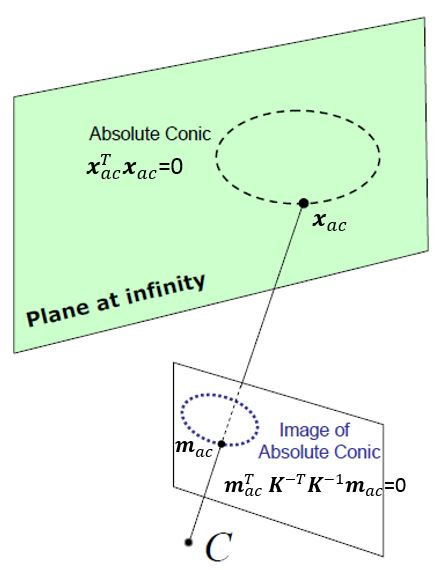
\includegraphics[scale=0.5]{AbsoluteConic}
    \caption{The absolute conic and the image of the absolute conic \cite{emerging}}
    \label{fig:absconic}
\end{figure}

Thus it is this conic of purely imaginary points that lies upon the plane at infinity. The importance of the absolute conic is that it is invariant under any Euclidean transformations. In other words the relative position of the absolute conic to a camera is unaffected by movement of the camera. Consider a point $\bm{x}_{ac}$ in Euclidean space in the world coordinate system that lies on the absolute conic. It has homogeneous coordinates $\tilde{\bm{x}}_{ac}=[\bm{x}_{ac}^T, 0]^T$ in projective space. Applying a rotation and translation to this point to obtain $\tilde{\bm{x}}_{ac}'$, which is equivalent to moving the camera in the world coordinate system, a corresponding point is obtained in the camera coordinate system.
\begin{align}
  \tilde{\bm{x}}_{ac}' &=
  \bm{V} \tilde{\bm{x}}_{ac} =
  \begin{bmatrix}
  \bm{R} & \bm{T} \\
  \bm{0} & 1
  \end{bmatrix}
  \tilde{\bm{x}}_{ac} =
  \begin{bmatrix}
  r_{11} & r_{12} & r_{13} & t_1 \\
  r_{21} & r_{22} & r_{23} & t_2 \\
  r_{31} & r_{32} & r_{33} & t_3 \\
  0 & 0 & 0 & 1
  \end{bmatrix}
  \begin{bmatrix}
  x_{ac} \\
  y_{ac} \\
  z_{ac} \\
  0
  \end{bmatrix} \\
  &= 
  \begin{bmatrix}
  \bm{R} \bm{x}_{ac} \\
  0
  \end{bmatrix}
\end{align}
It is clear that this point still lies on the plane at infinity since its $w$ is equal to zero. More importantly it can be proven that this point $\bm{x}_{ac}'$ is on the same absolute conic using the orthogonality of the rotation matrix $\bm{R}$.
\begin{equation}
  \bm{x}_{ac}'^T \bm{x}_{ac}' = \left( \bm{R} \bm{x}_{ac} \right) ^T \left( \bm{R} \bm{x}_{ac} \right) = \bm{x}_{ac}^T \bm{R}^T \bm{R} \bm{x}_{ac} = \bm{x}_{ac}^T \bm{R}^{-1} \bm{R} \bm{x}_{ac} = \bm{x}_{ac}^T \bm{x}_{ac} = 0
\end{equation}
Thus the absolute conic is invariant to Euclidean transformations. Now consider again a point, $\bm{x}_{ac}$, lying on the absolute conic. The corresponding point, $\bm{m}_{ac}$, in the sensor plane is given according to Equation \ref{eq:world 2 sensor}
\begin{align}
  \tilde{\bm{m}}_{ac} &=
  \frac{1}{\alpha} \bm{K} \bm{V}
  \begin{bmatrix}
  \bm{x}_{ac} \\
  0
  \end{bmatrix}=
   \frac{1}{\alpha} 
   \begin{bmatrix}
   f_x & f_s & c_x \\
   0 & f_y & c_y \\
   0 & 0 & 1 
   \end{bmatrix} 
  \begin{bmatrix}
  \bm{R} & \bm{T} \\
  \bm{0} & 1
  \end{bmatrix}
  \begin{bmatrix}
  \bm{x}_{ac} \\
  0
  \end{bmatrix} = \frac{1}{\alpha} \bm{K}
  \begin{bmatrix}
  \bm{R} \bm{x}_{ac} \\
  0
  \end{bmatrix} \\
  \therefore \bm{m}_{ac} &= \frac{1}{\alpha} \bm{K} \bm{R} \bm{x}_{ac}.
\end{align}
Checking whether this point satisfies equation \ref{eq:conditions of absolute conic} results in
\begin{equation}
  \bm{m}_{ac}^T \bm{K}^{-T} \bm{K}^{-1} \bm{m}_{ac} = \frac{1}{\alpha^2} \bm{x}_{ac}^T \bm{R}^T \bm{R} \bm{x}_{ac} = \frac{1}{\alpha^2} \bm{x}_{ac}^T \bm{x}_{ac} = 0
\end{equation}
Thus the image of the absolute conic is itself an absolute conic. \todo{absolute or imaginary conic?} The image of the absolute conic is defined by $\bm{K}^{-T} \bm{K}^{-1}$ \cite{luong1997self}. Thus since the image of the absolute conic is dependent only on intrinsic camera parameters it can be used to solve for the intrinsic camera parameters.

% http://www.cs.unc.edu/~marc/tutorial/node87.html
\subsection{Constraints on intrinsic parameters}
\label{sec: intrinsic constraints}
According to Zhang \cite{emerging} there are two constraints placed upon the intrinsic parameters of the camera. These are important later on in the solving for these intrinsic parameters. The plane of the calibration plate in the camera coordinate system is given by \cite{emerging} \todo{big t or small t}
\begin{equation}
  \begin{bmatrix}
  \bm{r}_3 \\
  \bm{r}_3^T \bm{T}
  \end{bmatrix}^T
  \begin{bmatrix}
  x_c \\
  y_c \\
  z_c \\
  w
  \end{bmatrix} = 0.
\end{equation}
Here $w$ is zero for points on the plane at infinity and one for those that are not. This plane intersects the plane at infinity on a line and it happens that $[\bm{r}_1^T, 0]^T$ and $[\bm{r}_2^T, 0]^T$ are two points on this line \cite{emerging}. Thus it is known that any point on this line, $\bm{x}_c^{\infty}$, is a linear combination of these two points.
\begin{equation}
  \bm{x}_c^{\infty} = a \begin{bmatrix}
  \bm{r}_1 \\
  0
  \end{bmatrix} + b
  \begin{bmatrix}
  \bm{r}_2 \\
  0
  \end{bmatrix} =
  \begin{bmatrix}
  a \bm{r}_1 + b \bm{r}_2 \\
  0
  \end{bmatrix}
\end{equation}
Now assume that this point, $\bm{x}_c^{\infty}$, lies on the absolute conic. Then this point must satisfy equation \ref{eq:conditions of absolute conic}. This would require that $a^2+b^2=0$ which results in the solution $b=\pm a i$, where $i=\sqrt{-1}$. As a result it can be seen that the two points along this line intersect the absolute conic at
\begin{equation}
  \bm{x}_c^{\infty} = a 
  \begin{bmatrix}
  \bm{r}_1 \pm i \bm{r_2} \\
  0
  \end{bmatrix}.
\end{equation}
Since these points lie on the absolute conic they are invariant under Euclidean transformations. Their projection, up to a scale factor, in the sensor coordinate system is given by \todo{added i to r in equation - make sure this is correct}
\begin{equation}
  \bm{x}_s^{\infty} = \bm{K} \left( \bm{r}_1 \pm i \bm{r}_2 \right) = \bm{h}_1 \pm i \bm{h}_2.
\end{equation}
\todo{check that i is correct - italics or not etc}
Here $\bm{h}_i = [h_{1i} \, h_{2i} \, h_{3i}]^T$ is the i\textsuperscript{th} column of the homography matrix. Substituting these points into equation \ref{eq:conditions of absolute conic} results in
\begin{equation}
  \left( \bm{h}_1 \pm i \bm{h}_2 \right)^T \bm{K}^{-T} \bm{K}^{-1} \left( \bm{h}_1 \pm i \bm{h}_2 \right) = 0.
\end{equation}
Enforcing this equation for both imaginary and real parts results in two constraints on the intrinsic parameters.
% Requiring both the imaginary and real parts of this equation to equal zero results in two constraints on the intrinsic parameters.
\begin{align}
  \label{eq:intrinsic constraints 1}
  \bm{h}_1^T \bm{K}^{-T} \bm{K}^{-1} \bm{h}_2 &= 0 \\
  \label{eq:intrinsic constraints 2}
  \bm{h}_1^T \bm{K}^{-T} \bm{K}^{-1} \bm{h}_1 &= \bm{h}_2^T \bm{K}^{-T} \bm{K}^{-1} \bm{h}_2
\end{align}
% Where $\bm{h}_i = [h_{i1} \, h_{i2} \, h_{i3}]^T$ is the i\textsuperscript{th} column of the homography matrix.

\subsection{Intrinsic parameters and the absolute conic}
\label{sec: parameters and the absolute conic}
Using DLT an homography, $\bm{H}$, between the calibration plate and the image of the calibration plate can be estimated. This homography can then be used to solve for the image of the absolute conic. Once the image of the absolute conic is known it can be used to solve for the intrinsic camera parameters. The image of the absolute conic can be represented as
\begin{equation}
  \bm{B} = \bm{K}^{-T} \bm{K}^{-1} = 
  \begin{bmatrix}
  b_{11} & b_{12} & b_{13}\\
  b_{12} & b_{22} & b_{23} \\
  b_{13} & b_{23} & b_{33}
  \end{bmatrix}
\end{equation}
Since $\bm{B}$ is symmetric its contents can be represented by a 6D vector $\bm{b}=[b_{11} \, b_{12} \, b_{22} \, b_{13} \, b_{23} \, b_{33}]^T$. Then using to Zhang's convention \cite{emerging}
\begin{equation}
  \bm{h}_i^T \bm{B} \bm{h}_j = \bm{q}_{ij} \bm{b}
\end{equation}
where 
\begin{equation}
  \bm{q}_{ij} = [ h_{i1} h_{j1}, h_{i1} h_{j2} + h_{i2} h_{j1}, h_{i2} h_{j2}, h_{i3} h_{j1} + h_{i1} h_{j3}, h_{i3} h_{j2} + h_{i2} h_{j3}, h_{i3} h_{j3}]^T.
\end{equation}
Then equations \ref{eq:intrinsic constraints 1} and \ref{eq:intrinsic constraints 2} can be rewritten as 
\begin{equation}
  \begin{bmatrix} 
  \bm{q}_{12}^T \\
  ( \bm{q}_{11} - \bm{q}_{22})^T
  \end{bmatrix} \bm{b} = \bm{0}
\end{equation}
A separate version of this equation exist for each image taken of the calibration plate and these equations can be stacked vertically, in $\bm{Q}$, to give
\begin{equation}
  \bm{Q}\bm{b}=\bm{0}.
\end{equation}
The solution for $\bm{b}$, up to a scale factor $\lambda$, is known to be the eigenvector of $\bm{Q}^T\bm{Q}$ associated with the smallest eigenvalue \cite{emerging}. Once $\bm{b}$ has been determined it can be used to determine the intrinsic parameters of the matrix $\bm{K}$. The relation between $\bm{B}$ and $\bm{K}$ is $\bm{B}=\lambda \bm{K}^{-T} \bm{K}^{-1}$. The intrinsic parameters are determined as follows.
\begin{align}
  c_y &= (b_{12} b_{13} - b_{11} b_{23})/(b_{11} b_{22} - b_{12}^2) \\
  \lambda &= b_{33} -(b_{13}^2 + c_y(b_{12} b_{13} - b_{11} b_{23}))/b_{11}\\
  f_x &= \sqrt{\frac{\lambda}{b_{11}}} \\
  f_y &= \sqrt{\frac{\lambda b_{11}}{b_{11} b_{22} - b_{12}^2}} \\
  f_s &= \frac{-b_{12} f_x^2 f_y}{\lambda} \\
  c_x &= \frac{f_s c_y}{f_y} - \frac{b_{13} f_x^2}{\lambda}
\end{align}
Thereafter the extrinsic parameters for each image can be determined separately using the appropriate homography matrix.
\begin{align}
  \bm{r}_1 &= \lambda \bm{K}^{-1} \bm{h}_1 \\
  \bm{r}_2 &= \lambda \bm{K}^{-1} \bm{h}_2 \\
  \bm{r}_3 &= \bm{r}_1 \times \bm{r}_2 \\
  \bm{T} &= \lambda \bm{K}^{-1} \bm{h}_3
\end{align}
% At this point it is necessary to incorporate distortions and use them to find better approximations for the intrinsic and extrinsic parameters.

\todo{this section is too close to the paper} %a fleixible new technique and reading 1
% by which the optical characteristics of a camera and the relation between its coordinate system and the world coordinate system are determined. It is performed in order to be able to extract \hl{metric} information from images accurately.

% \section{Closed form solution}
% Sections \ref{sec: homography} through to \ref{sec: parameters and the absolute conic} illustrate that estimates to the intrinsic and extrinsic parameters can be obtained by first determining the homographies for each calibration image, then these can be used to determine the image of the abolute conic which in turn can be used to determine the intrinsic and extrinsic camera parameters. This is closed form solution is the first part of the calibration process

% put inverse problem in calibration plate section

% explain homography and absolute conic

% then explain closed form solution and optimization - give closed form and explain optimization


\subsection{Distortion in Calibration}
Sections \ref{sec: homography} through \ref{sec: parameters and the absolute conic} outline the framework for determining the closed form solution of the calibration problem when distortion is not considered. The estimates for the extrinsic and intrinsic parameters obtained using this closed form solution need to be improved by accounting for distortion. 

As stated in Section \ref{sec: distortion} good calibration results are achieved by only taking radial distortion into account. This is beneficial since it is possible to estimate the radial distortion parameters using a closed form solution in a similar manner to how the intrinsic and extrinsic parameters are estimated.

% It is only once the closed form solution to the extrinsic and intrinsic parameters is optimised that distortion can be accounted for during the calibration process. 

% As already presented, there are many types of distortion that occur when an image is taken. However it is seldom possible to take all of these distortion types into account since the more distortion parameters introduced into the camera model; the more likely the optimization process becomes unstable.

% It has been found \todo{add reference for this} that good calibration results can be achieved by taking only radial distortion into account during calibration \cite{tsai1987versatile,wei1994implicit}. This is beneficial since it is possible to solve for initial guesses to the radial distortion parameters which helps the optimisation process to avoid local minima as a result of the distortion parameters used.

Taking into account two radial distortion parameters results in distortion being applied to the points on the image plane as
 % The distortion applied to the points on the image plane is of the form
\begin{align}
  \hat{\bm{X}}_{p_i} =
  \begin{bmatrix}
  \hat{x}_{p_i} \\
  \hat{y}_{p_i}
  \end{bmatrix} &= \left(
  1 + \kappa_1 r_i^2 + \kappa_2 r_i^4 \right)
  \begin{bmatrix}
  x_{p_i} \\
  y_{p_i}
  \end{bmatrix} =
  \left(
    1 + \kappa_1 r_i^2 + \kappa_2 r_i^4 \right) \bm{X}_{p_i} \\
  \text{where} \quad \quad r_i &= \sqrt{x_{p_i}^2 + y_{p_i}^2}
  \label{eq: distortion radius}
\end{align}
Here $\hat{\bm{X}}_{p_i} = \begin{bmatrix} \hat{x}_{p_i} & \hat{y}_{p_i} \end{bmatrix} ^T$ and $\bm{X}_{p_i} = \begin{bmatrix} x_{p_i} & y_{p_i} \end{bmatrix} ^T$ represent the distorted and undistorted image plane coordinates respectively.

At this point the intrinsic and extrinsic parameters have been determined using the pinhole camera model and the error between the predicted calibration plate targets and the actual location of these in the images is attributed to radial distortion \cite{zhangtut}. This error is represented as the observed distortion vector $\bm{d}_{1_i}$.
\begin{equation}
  \bm{d}_{1_i} = \bm{X}_{s_i}^{a} - \bm{X}_{s_i}^{c}
\end{equation}
Here $\bm{X}_{s_i}^{a}$ is the actual coordinates observed and $\bm{X}_{s_i}^{c}$ is the predicted coordinates that are calculated according to the camera model. These coordinates are in the sensor coordinate system. \todo{check bolding of vectors is correct}

According to Burger \cite{zhangtut} an undistorted point in the sensor coordinate system, $\bm{X}_{s_i}^c$ is distorted to point $\hat{\bm{X}}_{s_i}^c$ as
\begin{align}
  \hat{\bm{X}}_{s_i}^c &= \bm{U}_c + (\bm{X}_{s_i}^c-\bm{U}_c) (1 + \kappa_1 r_i^2 + \kappa_2 r_i^4) \\
  &= \bm{U}_c + \bm{X}_{s_i}^c - \bm{U}_c + (\bm{X}_{s_i}^c-\bm{U}_c) (\kappa_1 r_i^2 + \kappa_2 r_i^4) \\
  &= \bm{X}_{s_i}^c + (\bm{X}_{s_i}^c-\bm{U}_c) (\kappa_1 r_i^2 + \kappa_2 r_i^4) \\
  &= \bm{X}_{s_i} + \bm{d}_{2_i}
\end{align}

% According to Burger \cite{zhangtut} an undistorted point, $\bm{X_{p_i}}$ is distorted to point $\hat{\bm{X_{p_i}}}$ according to
% \begin{align}
%   \hat{\bm{X_{p_i}}} &= \bm{U_c} + (\bm{X_{p_i}}-\bm{U_c}) \times (1 + k_1 r_i^2 + k_2 r_i^4) \\
%   &= \bm{U_c} + \bm{X_{p_i}} - \bm{U_c} + (\bm{X_{p_i}}-\bm{U_c}) \times (k_1 r_i^2 + k_2 r_i^4) \\
%   &= \bm{X_{p_i}} + (\bm{X_{p_i}}-\bm{U_c}) \times (k_1 r_i^2 + k_2 r_i^4) \\
%   &= \bm{X_{p_i}} + \bm{d_{2_i}}
% \end{align}
Here $\bm{U}_c = \begin{bmatrix} u_c & v_c \end{bmatrix}^T$ is the projection centre or principal point (the intersection of the optical axis with the image plane) in the sensor coordinate system and is determined by applying Equation \ref{eq: image2sensor} to the principal point, $(0,0)$, given in terms of the image plane coordinate system. The term $\bm{d}_{2_i}$ is referred to as the model distortion vector. Note that $r_i$ used here is calculated according to Equation \ref{eq: distortion radius} using image plane coordinates.

The distortion parameters can be estimated by minimizing the difference between the model and observed distortion vectors. Thus the least squares solution to the overdetermined system of equations of the form $\bm{d}_{2_i} = \bm{d}_{1_i}$ is what is needed. For each point $\bm{X}_{s_i}^c$ considered there are two equations of the form
\begin{align}
  (x_{s_i}^c - u_c) \times (\kappa_1 r_i^2 + \kappa_2 r_i^4) &= (x_{s_i}^{a} - x_{s_i}^{c}) \\
  (y_{s_i}^c - v_c) \times (\kappa_1 r_i^2 + \kappa_2 r_i^4) &= (y_{s_i}^{a} - y_{s_i}^{c}).
\end{align}
Two equations of this form are created for each target of the calibration plate and these equations are then stacked into a system of equations which is used to solved for the least squares solution to the distortion parameters.
\begin{equation}
  \begin{bmatrix}
    (x_{s_1}^c - u_c) \times r_1^2 & (x_{s_1}^c - u_c) \times r_1^4\\
    (y_{s_1}^c - v_c) \times r_1^2 & (y_{s_1}^c - v_c) \times r_1^4\\
    (x_{s_2}^c - u_c) \times r_2^2 & (x_{s_2}^c - u_c) \times r_2^4\\
    (y_{s_2}^c - v_c) \times r_2^2 & (y_{s_2}^c - v_c) \times r_2^4\\
    \vdots & \vdots
  \end{bmatrix}
  \begin{bmatrix}
    \kappa_1 \\
    \kappa_2
  \end{bmatrix} =
  \begin{bmatrix}
    x_{s_1}^{a} - x_{s_1}^{c}\\
    y_{s_1}^{a} - y_{s_1}^{c}\\
    x_{s_2}^{a} - x_{s_2}^{c}\\
    y_{s_2}^{a} - y_{s_2}^{c}\\
    \vdots
  \end{bmatrix}
\end{equation}

\subsection{Non-linear optimisation}
At this point good approximations have been calculated for all the calibration parameters using closed form solution methods. However, since the correlation process relies upon the calibration process to link optical flow in images to displacement in the 3D world, these calibration parameters need to be refined so that they don't negatively affect the correlation results. 

First Equation \ref{eq:world 2 sensor} must be modified to incorporate radial distortion. Radial distortion is applied to the image plane coordinates prior to converting them to sensor coordinates. As such the conversion from world coordinates, $\bm{X}_w$, to distorted sensor coordinates, $\hat{\bm{X}}_s$, can be broken down into three functions as
\begin{align}
  \hat{\bm{X}}_s &= f_{ws}(\bm{X}_w,\bm{R},\bm{T},\gamma,\kappa_1,\kappa_2,S_x,S_y,\phi,\hat{c}_x,\hat{c}_y) \\
  &= f_{is}(f_{dist}(f_{wi}(\bm{X}_w,\bm{R},\bm{T},\gamma),\kappa_1,\kappa_2),S_x,S_y,\phi,\hat{c}_x,\hat{c}_y)
\end{align}
where $f_{ws}$ represents the function that converts from world to sensor coordinates, $f_{is}$ converts image plane coordinates to sensor coordinates, $f_{dist}$ distorts the image plane coordinates and $f_{wi}$ converts from world to image plane coordinates.

These functions are expanded as
\begin{align}
  f_{wi}(\bm{X}_w,\bm{R},\bm{T},\gamma) &= \bm{X}_p =
  \begin{bmatrix}
  \gamma & 0 & 0 & 0 \\
  0 & \gamma & 0 & 0 \\
  0 & 0 & 1 & 0
  \end{bmatrix}
  \begin{bmatrix}
  \bm{R} & \bm{T} \\
  \bm{0} & 1
  \end{bmatrix}
  \bm{X}_w \\
  f_{dist}(\bm{X}_p,\kappa_1,\kappa_2) &= \hat{\bm{X}}_p =
  \left( 1 + \kappa_1  (\bm{X}_p^T \bm{X}_p) + \kappa_2 (\bm{X}_p^T \bm{X}_p)^2 \right) \bm{X}_p \\
  f_{is}(\hat{\bm{X}}_p,S_x,S_y,\phi,\hat{c}_x,\hat{c}_y) &= \hat{\bm{X}}_s =
  \begin{bmatrix}
  S_x & -S_x \cot \phi & -S_x \left( \hat c_x - \hat c_y \cot \phi \right) \\
  0 & \frac{S_y}{\sin \phi} & -\frac{S_y \hat c_y}{\sin \phi} \\
  0 & 0 & 1
  \end{bmatrix}
  \hat{\bm{X}}_p.
\end{align}

This function, $f_{ws}$, is applied to the known calibration targets in the world coordinate system, $\bm{X}_w^a$, in order to predict where they will appear in the image, $\bm{X}_s^c$. However, since estimates of the intrinsic, extrinsic and distortion parameters are used, these calculated locations will differ from the actual locations of the calibration targets, $\bm{X}_s^a$. The absolute value of these differences are summed together to obtain the projection error, $P_{error}$.
\begin{equation}
  P_{error} = \sum_i^n \left| \bm{X}_{s_i}^a - \bm{X}_{s_i}^c \right| = \sum_i^n \left| \bm{X}_{s_i}^a - f_{ws}(\bm{X}_{w_i}^a,\bm{R},\bm{T},\gamma,\kappa_1,\kappa_2,S_x,S_y,\phi,\hat{c}_x,\hat{c}_y) \right|
\end{equation}

Consequently these estimated parameters need to be optimised using an iterative non-linear optimisation technique to complete the calibration process. Matlab's 'lsqnonlin' optimisation algorithm was chosen for this project. The aim of using this optimisation algorithm is to minimise the projection error by iteratively making improvements to the estimated parameters.

% This is done by combining the camera model and distortion into one mathematical relation that related 3D coordinates in the physical world to 2D coordinates in the images. It is important to note that the distortion model is inserted into the camera model prior to converting the image plane coordinates to the sensor plane coordinates. Thus the camera model becomes
% \begin{equation}
%   \bm{X_s}=\bm{K} D \bm{V} \bm{X_w}.
% \end{equation}
% This camera model and the approximations of the calibration parameters are employed in a non-linear optimization scheme in order to improve all of the calibration parameters simultaneously. Matlab's built in Levenberg-Marquart non-linear least squares optimisation algorithm was used for this. The sum of the absolute of the difference between the calculated and observed calibration plate targets was used as a measure of the error for the algorithm.

% However these estimates need to be improved upon in order to obtain the true calibration parameter values. This is done by using a non-linear optimisation scheme in order to improve all of the parameters simultaneously. Thus the camera model is combined with the distortion model to obtain one mathematical model of the image capturing system. The Levenberg-Marquart non-linear least squares optimisation algorithm was used to iteratively improve the calibration parameters.

\section{Correspondence problem}
\label{sec: correspondence problem}
The purpose of DIC is to solve the correspondence problem between two images. The correspondence problem refers to solving for the apparent motion that an object, within a set of images, experiences from one image to the next. For example consider a traffic camera that records images of a car at an intersection. If someone were to review these images the apparent motion of the car between images would be obvious. 

% This is because humans are incredibly adapt at solving the correspondence problem through pattern recognition. Computers can also be used to solve the correspondence problem, and to much greater accuracy than a human, however they need the correspondence problem to be well defined. The way in which the correspondence problem is defined determines what type of DIC algorithm is used to solve it. 

This is because humans are incredibly adapt at solving the correspondence problem through pattern recognition. Computers can also be used to solve the correspondence problem, and to much greater accuracy than a human, however they need the correspondence problem to be broken down into a well defined mathematical problem. The way in which the correspondence problem is broken down into a mathematical problem determines what type of DIC algorithm is used to solve it. 

% however they need the correspondence problem to be broken down into a well defined mathematical problem. The way in which the correspondence problem is broken down into a mathematical problem determines what type of DIC algorithm is used to solve it. 

% however they need the correspondence problem to be broken down into a well framed problem. The way in which the correspondence problem is defined determines what type of DIC algorithm is used to solve it. 

This project is focused on using DIC for material testing where the deformation experienced by a loaded specimen needs to be measured. As such it is not the overall motion of the specimen that is sought for but the motion that portions of the specimen experience as a result of the stresses within the specimen. Therefore in this project the correspondence problem is broken down as tracking the pattern contained within a cluster of neighbouring pixels from one image to the next.

This cluster of neighbouring pixels is termed a subset and a subset spans a small portion of the specimen being imaged. Thus, by tracking the motion of many subsets that together span the whole surface of the specimen, the deformation of the specimen can be measured. The DIC algorithms that are used to solve this type of correspondence problem are termed subset-based DIC algorithms.

\subsection{Speckle pattern}
Tracking of subsets in this way places requirements on the patterns contained within the subsets. %This is because a subset can only be tracked reliably if the pattern it contains is unique. 
To illustrate this consider a checker board pattern which is a repeated pattern of alternating black and white squares of constant size. An image is taken of this pattern in the reference position and another is taken after the pattern has been displaced to the right by a distance equal to two and a half times the length of one of the sides of the squares.

Treating the whole first image as a single subset the displacement between the two images can be calculated. However this calculated displacement will be half the length of one of the sides of the squares. This is because if the first image is displaced by this amount it will be identical to the second image even though the true displacement between the images is much greater.

Thus it is clear that the pattern to be tracked in the images can have a significant impact on the performance of the correlation process. According to Sutton \cite{sutton2009image} for the best results the pattern contained within the images should be isotropic and non-periodic. This is achieved by applying a random speckle pattern to the surface of the specimen to be tested since these provide very unique patterns which are isotropic in nature. Additionally their high information density enables smaller subsets to be used which allows the deformation of the specimen to be measured with more detail.



% Since this project is focused on using DIC for material testing where motion between images is relatively small 

% where it is not the motion of an object but the motion that sections of the object experience.

% This cluster of neighbouring pixels is termed a subset. By breaking down the corr problem in this way the object to be tracked becomes the pattern contained within a subset

% The purpose of using subsets is that the whole image can be broken down into many pieces 

% However the correspondence problem is harder for computers to solve

% However computers can also solve the correspondence problem and to much greater accuracy than a human.

% That is to determine the motion experienced by an object from one image to the next. 

corr problem
subsets
speckle patterns 

\section{Correlation}
Correlation is the process of solving the correspondence problem between two images. According to how the correspondence problem was broken down in Section \ref{sec: correspondence problem} correlation determines how the pattern within a subset of one image, the reference image, needs to be displaced and deformed such that it matches the corresponding pattern in another image, the deformed image.

% The correspondence problem was broken down in Section \ref{sec: correspondence problem} as tracking the pattern contained within subset from one image to the next. Therefore correlation is a process that determines how the pattern within a subset of one image, the reference image, needs to be displaced and deformed such that it matches the corresponding pattern in another image, the deformed image. 

However the correspondence problem first needs to be mathematically defined before it can be solved. There are four elements that together mathematically define the correspondence problem. These are the warp function, correlation criteria, interpolation method and optimisation algorithm. These elements are discussed in the sections that follow.

% Therefore the DIC algorithms that are used to solve for this displacement and deformation are referred to as subset-based DIC algorithms which indicates the way in which the correspondence problem has been broken down.

% Using this as the framework for the correspondence problem the 

% Although the correspondence problem was stated in Section \ref{sec: correspondence problem} as tracking the pattern contained within subset from one image to the next, this does not fully define the correspondence problem. 


% correspondence problem not fully defined
% talk about how needs to be mathematically defined
\subsection{Warp function}
% The warp function is an equation that defines how a subset can displace and deform between images. Thus the warp function determines what 

When applying DIC to material science the deformation behaviour of materials under load must be taken into account. This is because the deformation of the material causes the speckle pattern on its surface to deform in the same way. This is an issue since the pattern contained within a subset of the reference image will be deformed in the second image which can cause difficulties in matching the two subsets.

This is solved by allowing the subsets to deform in a similar way to that of the material by defining the allowable deformations in a warp function. The purpose of the warp function is to transform the pixel coordinates of a subset in one image so that the resulting pattern is closer to the pattern contained in another image. The most popular warp function in material science is the first order warp function which accounts for affine transformations. It is popular because its parameters are closely related to the strains used to characterise material deformation. Thus by determining the warp function parameters for a specific subset; the strains experienced by that subset are also determined. This warp function is given as

% This is solved by allowing the subsets to deform in a similar way to that of the material by defining the allowable deformations in a warp function. The purpose of these warp functions is to transform the pixel coordinates of the reference subset so that the resulting pattern is closer to the pattern in the deformed image. The most popular warp function in material science is the first order warp function which accounts for affine transformations. It is popular because its parameters are closely related to the strains used to characterise material deformation. Thus by determining the warp function parameters for a specific subset; the strains experienced by that subset are also determined. This warp function is given as

% For this analysis the common warp function which accounts for affine transformations is used since it is consistent with the strains that the material is expected to experience. Thus by determining the warp function parameters for a specific subset; the strains for that subset are also determined.
\begin{equation}
  W (\bm{\zeta},\bm{p}) = 
  \begin{bmatrix}
  \Delta x_{warp} \\
  \Delta y_{warp}
  \end{bmatrix} 
  = \begin{bmatrix}
  1+\frac{\partial u}{\partial x} & \frac{\partial u}{\partial y} & u\\
  \frac{\partial v}{\partial x} & 1+\frac{\partial v}{\partial y} & v 
  \end{bmatrix}
  \begin{bmatrix}
  \Delta x \\
  \Delta y \\
  1
  \end{bmatrix}.
  \label{eq:warp}
\end{equation}
Here $u$ and $v$ represent the displacements in the x and y directions respectively, $\frac{\partial u}{\partial x}$ and $\frac{\partial v}{\partial y}$ represent the elongation in the x and y directions respectively whereas $\frac{\partial v}{\partial x}$ and $\frac{\partial u}{\partial y}$ represent the shear deformation of the subset. All of these variables are stored within the vector $\bm{p}$ and are referred to as the warp function parameters (WFPs). The WFPs define how the subset is warped and are stored as
\begin{equation}
  \bm{p} = \begin{bmatrix} u & \frac{\partial u}{\partial x} & \frac{\partial u}{\partial y} & v & \frac{\partial v}{\partial x} & \frac{\partial v}{\partial y} \end{bmatrix} = \begin{bmatrix} p_1 & p_2 & p_3 & p_4 & p_5 & p_6 \end{bmatrix}
\end{equation}

% All of these variables, which are referred to as the warp function parameters, are stored within the vector $\bm{p} = \begin{bmatrix} u & \frac{\partial u}{\partial x} & \frac{\partial u}{\partial y} & v & \frac{\partial v}{\partial x} & \frac{\partial v}{\partial y} \end{bmatrix}$. These parameters define how the subset is warped.

Additionally $\Delta x$ and $\Delta y$ are the distances from the centre of the undeformed subset to the pixel under consideration and are contained within the variable $\bm{\zeta} = \begin{bmatrix} \Delta x & \Delta y & 1 \end{bmatrix}^T$. The outputs $\Delta x_{warp}$ and $\Delta y_{warp}$ are the modified distances from the centre of the subset to the pixel under consideration. 
% Thus it is the pixel locations within the subset that are modified in order to induce warp and not the subset itself which is warped by this function. In other words the $\Delta x$ and $\Delta y$ are warped by the function which has the effect of warping the subset itself since it changes the locations within the subset that are to be evaluated. Thus the warp function applied to a subset is mathematically expressed as
Thus it is the pixel locations within the subset that are modified in order to induce warp and not the subset itself which is warped by this function. In other words the subset's shape remains the same but the pattern contained within the subset warps as a results of sampling the light intensity values of the image at warped locations. Thus the warp function applied to a subset is mathematically expressed as
%, $(x_0 + \Delta x_{warp},y_0 + \Delta y_{warp})$. 

% In other words the $\Delta x$ and $\Delta y$ are warped by the function which has the effect of warping the subset itself since it changes the locations within the subset that are to be evaluated. Thus the warp function applied to a subset is mathematically expressed as

\begin{equation}
  G_{warped}=G(\bm{x_0}+W(\bm{\zeta},\bm{p}))
  \label{eq:subset warp}
\end{equation}
where $\bm{x_0} = \begin{bmatrix} x_0 & y_0 \end{bmatrix}^T$ are the x and y coordinates, in units of pixels, of the centre of the subset. 

% With most subset based DIC algorithms the more complex the warp function becomes the more computationally expensive each iteration is. This is because the correlation criteria must be optimized in terms of more variables leading to more work. \todo{keep this?}
% http://sci-hub.tw/http://www.mdpi.com/1424-8220/18/4/1208/htm
% https://www.ncbi.nlm.nih.gov/pubmed/29659492

\subsection{Correlation criteria}
A correlation criteria is a mathematical way of quantifying how well a subset in one image matches a subset in another image. It is used to calculate the correlation coefficient which indicates whether the WFPs, that have been solved for, are sufficiently accurate to explain how a subset in the reference image is related to the deformed image. Furthermore the correlation criteria is usually used as the basis for the optimisation algorithm that performs the correlation process.
% Furthermore the correlation criteria is usually used as the basis for the iterative solve that performs the correlation process.
As such it is important that the correlation criteria reliably indicates the fit between the two subsets.

This reliability refers to dealing with the changes in lighting between images. As images are taken, as the specimen is deformed, the light intensity of the images can change as a result of changes in lighting, changes in reflectivity as the material strains and so on. Although this does not cause the patterns in the subsets to change it does cause the grayscale values of individual pixels, that make up these patterns, to change which can negatively affect the correlation process. The changes in lighting that takes place between images have been categorised into two types; offset and scaling. 

% The first is offset in light intensities which is dealt with by using zero-mean normalisation. Zero-mean normalisation determines the mean intensity value of a subset and then subtracts that mean intensity from every pixel in that subset.
% \begin{align}
%   G_{i}^{ZN} &= G_i - \mean{G}\\
%   \text{where} \quad \mean{G} &= \frac{\sum_{i}^{n} G_{i}}{n}
% \end{align}

% The second is scaling of the light intensity values between images. This corrected for by dividing the correlation criteria determined by the 

The two most commonly used correlation criteria are the Cross-Correlation and Sum of Squared difference criteria. Each of these has four versions for dealing with various combinations of light intensity changes.

\subsubsection{Cross-Correlation}
The cross-correlation criteria obtains a coefficient by multiplying each element of the reference subset with its corresponding element in the investigated subset, of the deformed image, and then summing all of these values together as shown below. Thus a higher value means better correlation.
\begin{equation}
  C_{CC} = \sum_{i}^n F_i G_i
\end{equation}
Here $n$ is the number of pixels contained within a subset.
This correlation criteria can be modified to be capable of dealing with offsets in light intensity by using zero-mean normalisation. Zero-mean normalisation determines the mean intensity value of a subset and then subtracts that mean intensity from every pixel in that subset. This is done for both subsets to obtain the Zero-Mean Cross-Correlation as shown below.
\begin{align}
  C_{ZCC} = \sum_i^n \left( F_i - \mean{F} \right) \left( G_i - \mean{G} \right) \\
  \text{where} \quad \mean{F} = \frac{\sum_{i}^{n} F_{i}}{n} \quad
   \text{and} \quad \mean{G} =\frac{\sum_{i}^{n} G_{i}}{n}
\end{align}

The correlation criteria can also be modified to deal with scaling of light intensities by dividing it by the root-sum-square of the subset's intensities. This is referred to as Normalised Cross-Correlation. 
\begin{align}
  C_{NCC} = \frac{\sum_i^n F_i G_i}{\sqrt{\sum_i^n F_i^2 \sum_i^n G_i^2}}
\end{align}

Both of these methods can be combined together to obtain Zero-Mean Normalised Cross-Correlation which is insensitive to both scaling and offset.
\begin{equation}
  C_{ZNCC} = \frac{\sum_i^n (F_i - \mean{F}) (G_i - \mean{G} )}{\sqrt{\sum_i^n (F_i - \mean{F})^2 \sum_i^n (G_i - \mean{G})^2}}
\end{equation}

\subsubsection{Sum of Squared Difference}
As the name suggests this correlation criteria is based on summing the square of the differences between the light intensities of the reference and the investigated subsets.
\begin{equation}
  C_{SSD} = \sum_i^n \left( F_i - G_i \right)^2 \label{eq: ssd}
\end{equation}
Since this correlation criteria measures differences; a smaller value means better correlation between the subsets. This correlation criteria can be modified in the same way to become insensitive to both offset (Zero-Mean Sum of Squared Difference) and scaling (Normalised Sum of Squared Difference).
\begin{align}
  C_{ZSSD} &= \sum_i^n \left[ \left( F_i - \mean{F} \right) - \left( G_i - \mean{G} \right) \right]^2 \label{eq: zssd} \\
  C_{NSSD} &= \sum_i^n \left[ \frac{F_i}{\sqrt{\sum_i^n F_i^2}} - \frac{G_i}{\sqrt{\sum_i^n G_i^2}} \right]^2 \label{eq: nssd}
\end{align}

These can then be combined to obtain the Zero-Mean Normalised Sum of Squared Difference correlation criteria which is insensitive to both scaling and offset in light intensities.
\begin{equation}
\label{eq: ZNSSD}
  C_{ZNSSD} = \sum_i^n \left[ \frac{F_i - \mean{F}}{\sqrt{\sum_i^n (F_i - \mean{F})^2}} - \frac{G_i - \mean{G}}{\sqrt{\sum_i^n (G_i - \mean{G})^2}} \right]^2
\end{equation}

\subsubsection{Relation between ZNCC and ZNSSD}
It can be shown that the Zero-Mean Normalised Cross-Correlation and Zero-Mean Normalised Sum of Squared Difference correlation criteria are related.
\begin{align}
  C_{ZNSSD} &= \sum_i^n \left[ \frac{F_i - \mean{F}}{\sqrt{\sum_i^n (F_i-\mean{F})^2}} - \frac{G_i - \mean{G}}{\sqrt{\sum_i^n (G_i-\mean{G})^2}} \right]^2 \\
  &= \sum_i^n \left( \frac{(F_i-\mean{F})^2}{\sum_i^n (F_i-\mean{F})^2} - 2 \frac{(F_i-\mean{F})(G_i-\mean{G})}{\sqrt{\sum_i^n (F_i-\mean{F})^2} \sqrt{\sum_i^n (G_i-\mean{G})^2}} + \frac{(G_i-\mean{G})^2}{\sum_i^n (G_i-\mean{G})^2} \right) \\
  &= \frac{\sum_i^n(F_i-\mean{F})^2}{\sum_i^n (F_i-\mean{F})^2} + \frac{\sum_i^n (G_i-\mean{G})^2}{\sum_i^n (G_i-\mean{G})^2} - 2 \frac{\sum_i^n(F_i-\mean{F})(G_i-\mean{G})}{\sqrt{\sum_i^n (F_i-\mean{F})^2} \sqrt{\sum_i^n (G_i-\mean{G})^2}}\\
  &= 2 \left( 1- C_{ZNCC} \right)
\end{align}
This is significant since the ZNSSD criteria is easier to calculate while the ZNCC criteria value is easier to interpret. Thus it is common practice to calculate the ZNSSD criteria coefficient and convert it to the ZNCC value for easier interpretation.
\todo{slightly different from Czncc, make sure equal}

\subsection{Interpolation}
It is clear that warping a subset according to equation \ref{eq:subset warp} requires that the light intensity values between pixel locations be determined. This is an issue because images store this information in a discrete manner. This is solved by using interpolation to determine the light intensity values between pixels based on the light intensity values of neighbouring pixels. There are multiple interpolation algorithms that can be employed for this purpose each offering varying degrees of accuracy and computational efficiency. 

Computational efficiency is important since image interpolation is typically the most time consuming part of the correlation process for iterative sub-pixel DIC algorithms \cite{pan2016performance}. Additionally the interpolation algorithm needs to be accurate enough to give reliable estimates such that it does not itself introduce bias into the warped subset it calculates. With this taken into account the bicubic interpolation algorithm was chosen since it offers a good balance between computational efficiency and accuracy.
\begin{figure}[H]
    \centering
    \resizebox{0.6\linewidth}{!}{
    % This file was created by matlab2tikz.
%
%The latest updates can be retrieved from
%  http://www.mathworks.com/matlabcentral/fileexchange/22022-matlab2tikz-matlab2tikz
%where you can also make suggestions and rate matlab2tikz.
%
\definecolor{mycolor1}{rgb}{0.00000,1.00000,1.00000}%
\definecolor{mycolor2}{rgb}{1.00000,0.00000,1.00000}%
%
\begin{tikzpicture}

\begin{axis}[%
width=4.521in,
height=3.566in,
at={(0.758in,0.481in)},
scale only axis,
xmin=-1,
xmax=2,
xtick={-1,  0,  1,  2},
tick align=outside,
xlabel style={font=\color{white!15!black}},
xlabel={x [pixels]},
ymin=-1,
ymax=2,
ytick={-1,  0,  1,  2},
ylabel style={font=\color{white!15!black}},
ylabel={y [pixels]},
zmin=0,
zmax=0.7,
zlabel style={font=\color{white!15!black}},
zlabel={Light intensity},
view={-18}{22},
axis background/.style={fill=white},
axis x line*=bottom,
axis y line*=left,
axis z line*=left,
xmajorgrids,
ymajorgrids,
zmajorgrids,
legend style={at={(0.272,0.772)}, anchor=south west, legend cell align=left, align=left, draw=white!15!black}
]
\addplot3 [color=mycolor1]
 table[row sep=crcr] {%
-1	-1	0.51\\
-0.96969696969697	-1	0.499043325820185\\
-0.939393939393939	-1	0.488590867351198\\
-0.909090909090909	-1	0.478632607062359\\
-0.878787878787879	-1	0.46915852742299\\
-0.848484848484849	-1	0.460158610902413\\
-0.818181818181818	-1	0.451622839969947\\
-0.787878787878788	-1	0.443541197094916\\
-0.757575757575758	-1	0.43590366474664\\
-0.727272727272727	-1	0.42870022539444\\
-0.696969696969697	-1	0.421920861507638\\
-0.666666666666667	-1	0.415555555555556\\
-0.636363636363636	-1	0.409594290007513\\
-0.606060606060606	-1	0.404027047332833\\
-0.575757575757576	-1	0.398843810000835\\
-0.545454545454545	-1	0.394034560480842\\
-0.515151515151515	-1	0.389589281242174\\
-0.484848484848485	-1	0.385497954754153\\
-0.454545454545455	-1	0.381750563486101\\
-0.424242424242424	-1	0.378337089907338\\
-0.393939393939394	-1	0.375247516487186\\
-0.363636363636364	-1	0.372471825694966\\
-0.333333333333333	-1	0.37\\
-0.303030303030303	-1	0.367822021871609\\
-0.272727272727273	-1	0.365927873779114\\
-0.242424242424242	-1	0.364307538191836\\
-0.212121212121212	-1	0.362950997579097\\
-0.181818181818182	-1	0.361848234410218\\
-0.151515151515151	-1	0.36098923115452\\
-0.121212121212121	-1	0.360363970281326\\
-0.0909090909090909	-1	0.359962434259955\\
-0.0606060606060606	-1	0.35977460555973\\
-0.0303030303030303	-1	0.359790466649971\\
0	-1	0.36\\
0.0303030303030303	-1	0.360393188079139\\
0.0606060606060606	-1	0.360960013356708\\
0.0909090909090908	-1	0.361690458302029\\
0.121212121212121	-1	0.362574505384423\\
0.151515151515152	-1	0.363602137073211\\
0.181818181818182	-1	0.364763335837716\\
0.212121212121212	-1	0.366048084147258\\
0.242424242424242	-1	0.367446364471158\\
0.272727272727273	-1	0.368948159278738\\
0.303030303030303	-1	0.370543451039319\\
0.333333333333333	-1	0.372222222222222\\
0.363636363636364	-1	0.373974455296769\\
0.393939393939394	-1	0.375790132732282\\
0.424242424242424	-1	0.37765923699808\\
0.454545454545455	-1	0.379571750563486\\
0.484848484848485	-1	0.381517655897821\\
0.515151515151515	-1	0.383486935470407\\
0.545454545454545	-1	0.385469571750564\\
0.575757575757576	-1	0.387455547207613\\
0.606060606060606	-1	0.389434844310877\\
0.636363636363636	-1	0.391397445529677\\
0.666666666666667	-1	0.393333333333333\\
0.696969696969697	-1	0.395232490191168\\
0.727272727272727	-1	0.397084898572502\\
0.757575757575758	-1	0.398880540946657\\
0.787878787878788	-1	0.400609399782954\\
0.818181818181818	-1	0.402261457550714\\
0.848484848484848	-1	0.403826696719259\\
0.878787878787879	-1	0.40529509975791\\
0.909090909090909	-1	0.406656649135988\\
0.939393939393939	-1	0.407901327322815\\
0.96969696969697	-1	0.409019116787712\\
1	-1	0.41\\
1.03030303030303	-1	0.410833959429001\\
1.06060606060606	-1	0.411510977544035\\
1.09090909090909	-1	0.412021036814425\\
1.12121212121212	-1	0.412354119709492\\
1.15151515151515	-1	0.412500208698556\\
1.18181818181818	-1	0.412449286250939\\
1.21212121212121	-1	0.412191334835963\\
1.24242424242424	-1	0.411716336922949\\
1.27272727272727	-1	0.411014274981217\\
1.3030303030303	-1	0.41007513148009\\
1.33333333333333	-1	0.408888888888889\\
1.36363636363636	-1	0.407445529676935\\
1.39393939393939	-1	0.405735036313549\\
1.42424242424242	-1	0.403747391268052\\
1.45454545454545	-1	0.401472577009767\\
1.48484848484848	-1	0.398900576008014\\
1.51515151515152	-1	0.396021370732115\\
1.54545454545455	-1	0.39282494365139\\
1.57575757575758	-1	0.389301277235162\\
1.60606060606061	-1	0.385440353952751\\
1.63636363636364	-1	0.381232156273479\\
1.66666666666667	-1	0.376666666666667\\
1.6969696969697	-1	0.371733867601636\\
1.72727272727273	-1	0.366423741547709\\
1.75757575757576	-1	0.360726270974205\\
1.78787878787879	-1	0.354631438350447\\
1.81818181818182	-1	0.348129226145755\\
1.84848484848485	-1	0.341209616829452\\
1.87878787878788	-1	0.333862592870857\\
1.90909090909091	-1	0.326078136739294\\
1.93939393939394	-1	0.317846230904082\\
1.96969696969697	-1	0.309156857834544\\
2	-1	0.3\\
};
 \addlegendentry{Bicubic surface}

\addplot3 [color=red, draw=none, mark=*, mark options={solid, fill=red, red}]
 table[row sep=crcr] {%
0.4	0.4	0.43674976\\
};
 \addlegendentry{Query point}


\addplot3[area legend, draw=black, fill=green, fill opacity=0.3]
table[row sep=crcr] {%
x	y	z\\
0	0	0\\
0	1	0\\
1	1	0\\
1	0	0\\
}--cycle;
\addlegendentry{Query area}

\addplot3 [color=mycolor1]
 table[row sep=crcr] {%
-1	0	0.45\\
-0.96969696969697	0	0.447497147786404\\
-0.939393939393939	0	0.445137880179203\\
-0.909090909090909	0	0.442918858001503\\
-0.878787878787879	0	0.440836742076412\\
-0.848484848484849	0	0.438888193227036\\
-0.818181818181818	0	0.437069872276484\\
-0.787878787878788	0	0.435378440047862\\
-0.757575757575758	0	0.433810557364276\\
-0.727272727272727	0	0.432362885048836\\
-0.696969696969697	0	0.431032083924646\\
-0.666666666666667	0	0.429814814814815\\
-0.636363636363636	0	0.428707738542449\\
-0.606060606060606	0	0.427707515930656\\
-0.575757575757576	0	0.426810807802543\\
-0.545454545454545	0	0.426014274981217\\
-0.515151515151515	0	0.425314578289785\\
-0.484848484848485	0	0.424708378551354\\
-0.454545454545455	0	0.424192336589031\\
-0.424242424242424	0	0.423763113225923\\
-0.393939393939394	0	0.423417369285138\\
-0.363636363636364	0	0.423151765589782\\
-0.333333333333333	0	0.422962962962963\\
-0.303030303030303	0	0.422847622227788\\
-0.272727272727273	0	0.422802404207363\\
-0.242424242424242	0	0.422823969724796\\
-0.212121212121212	0	0.422908979603195\\
-0.181818181818182	0	0.423054094665665\\
-0.151515151515151	0	0.423255975735315\\
-0.121212121212121	0	0.423511283635251\\
-0.0909090909090909	0	0.42381667918858\\
-0.0606060606060606	0	0.42416882321841\\
-0.0303030303030303	0	0.424564376547848\\
0	0	0.425\\
0.0303030303030303	0	0.425472354397974\\
0.0606060606060606	0	0.425978100564877\\
0.0909090909090908	0	0.426513899323817\\
0.121212121212121	0	0.427076411497899\\
0.151515151515152	0	0.427662297910232\\
0.181818181818182	0	0.428268219383922\\
0.212121212121212	0	0.428890836742076\\
0.242424242424242	0	0.429526810807803\\
0.272727272727273	0	0.430172802404207\\
0.303030303030303	0	0.430825472354398\\
0.333333333333333	0	0.431481481481482\\
0.363636363636364	0	0.432137490608565\\
0.393939393939394	0	0.432790160558756\\
0.424242424242424	0	0.43343615215516\\
0.454545454545455	0	0.434072126220887\\
0.484848484848485	0	0.434694743579041\\
0.515151515151515	0	0.435300665052731\\
0.545454545454545	0	0.435886551465064\\
0.575757575757576	0	0.436449063639146\\
0.606060606060606	0	0.436984862398086\\
0.636363636363636	0	0.437490608564989\\
0.666666666666667	0	0.437962962962963\\
0.696969696969697	0	0.438398586415115\\
0.727272727272727	0	0.438794139744553\\
0.757575757575758	0	0.439146283774383\\
0.787878787878788	0	0.439451679327712\\
0.818181818181818	0	0.439706987227648\\
0.848484848484848	0	0.439908868297298\\
0.878787878787879	0	0.440053983359768\\
0.909090909090909	0	0.440138993238167\\
0.939393939393939	0	0.4401605587556\\
0.96969696969697	0	0.440115340735175\\
1	0	0.44\\
1.03030303030303	0	0.439811197373181\\
1.06060606060606	0	0.439545593677825\\
1.09090909090909	0	0.43919984973704\\
1.12121212121212	0	0.438770626373932\\
1.15151515151515	0	0.438254584411609\\
1.18181818181818	0	0.437648384673178\\
1.21212121212121	0	0.436948687981746\\
1.24242424242424	0	0.43615215516042\\
1.27272727272727	0	0.435255447032307\\
1.3030303030303	0	0.434255224420514\\
1.33333333333333	0	0.433148148148148\\
1.36363636363636	0	0.431930879038317\\
1.39393939393939	0	0.430600077914128\\
1.42424242424242	0	0.429152405598687\\
1.45454545454545	0	0.427584522915101\\
1.48484848484848	0	0.425893090686479\\
1.51515151515152	0	0.424074769735927\\
1.54545454545455	0	0.422126220886552\\
1.57575757575758	0	0.42004410496146\\
1.60606060606061	0	0.417825082783761\\
1.63636363636364	0	0.415465815176559\\
1.66666666666667	0	0.412962962962963\\
1.6969696969697	0	0.41031318696608\\
1.72727272727273	0	0.407513148009016\\
1.75757575757576	0	0.404559506914879\\
1.78787878787879	0	0.401448924506776\\
1.81818181818182	0	0.398178061607814\\
1.84848484848485	0	0.3947435790411\\
1.87878787878788	0	0.391142137629741\\
1.90909090909091	0	0.387370398196844\\
1.93939393939394	0	0.383425021565518\\
1.96969696969697	0	0.379302668558867\\
2	0	0.375\\
};
 \addplot3 [color=mycolor1]
 table[row sep=crcr] {%
-1	1	0.52\\
-0.96969696969697	1	0.512018810696497\\
-0.939393939393939	1	0.504433313854802\\
-0.909090909090909	1	0.497235161532682\\
-0.878787878787879	1	0.490416005787907\\
-0.848484848484849	1	0.483967498678243\\
-0.818181818181818	1	0.477881292261458\\
-0.787878787878788	1	0.47214903859532\\
-0.757575757575758	1	0.466762389737596\\
-0.727272727272727	1	0.461712997746056\\
-0.696969696969697	1	0.456992514678465\\
-0.666666666666667	1	0.452592592592593\\
-0.636363636363636	1	0.448504883546206\\
-0.606060606060606	1	0.444721039597073\\
-0.575757575757576	1	0.441232712802961\\
-0.545454545454545	1	0.438031555221638\\
-0.515151515151515	1	0.435109218910872\\
-0.484848484848485	1	0.43245735592843\\
-0.454545454545455	1	0.430067618332081\\
-0.424242424242424	1	0.427931658179592\\
-0.393939393939394	1	0.426041127528731\\
-0.363636363636364	1	0.424387678437265\\
-0.333333333333333	1	0.422962962962963\\
-0.303030303030303	1	0.421758633163592\\
-0.272727272727273	1	0.42076634109692\\
-0.242424242424242	1	0.419977738820714\\
-0.212121212121212	1	0.419384478392743\\
-0.181818181818182	1	0.418978211870774\\
-0.151515151515151	1	0.418750591312575\\
-0.121212121212121	1	0.418693268775913\\
-0.0909090909090909	1	0.418797896318558\\
-0.0606060606060606	1	0.419056125998275\\
-0.0303030303030303	1	0.419459609872833\\
0	1	0.42\\
0.0303030303030303	1	0.420668948437544\\
0.0606060606060606	1	0.421458107243231\\
0.0909090909090908	1	0.422359128474831\\
0.121212121212121	1	0.423363664190111\\
0.151515151515152	1	0.424463366446838\\
0.181818181818182	1	0.42564988730278\\
0.212121212121212	1	0.426914878815705\\
0.242424242424242	1	0.428249993043382\\
0.272727272727273	1	0.429646882043576\\
0.303030303030303	1	0.431097197874057\\
0.333333333333333	1	0.432592592592593\\
0.363636363636364	1	0.43412471825695\\
0.393939393939394	1	0.435685226924896\\
0.424242424242424	1	0.4372657706542\\
0.454545454545455	1	0.43885800150263\\
0.484848484848485	1	0.440453571527952\\
0.515151515151515	1	0.442044132787934\\
0.545454545454545	1	0.443621337340346\\
0.575757575757576	1	0.445176837242953\\
0.606060606060606	1	0.446702284553524\\
0.636363636363636	1	0.448189331329827\\
0.666666666666667	1	0.44962962962963\\
0.696969696969697	1	0.451014831510699\\
0.727272727272727	1	0.452336589030804\\
0.757575757575758	1	0.453586554247711\\
0.787878787878788	1	0.454756379219189\\
0.818181818181818	1	0.455837716003005\\
0.848484848484848	1	0.456822216656927\\
0.878787878787879	1	0.457701533238723\\
0.909090909090909	1	0.458467317806161\\
0.939393939393939	1	0.459111222417008\\
0.96969696969697	1	0.459624899129031\\
1	1	0.46\\
1.03030303030303	1	0.460228177087681\\
1.06060606060606	1	0.460301082449843\\
1.09090909090909	1	0.460210368144252\\
1.12121212121212	1	0.459947686228678\\
1.15151515151515	1	0.459504688760887\\
1.18181818181818	1	0.458873027798648\\
1.21212121212121	1	0.458044355399727\\
1.24242424242424	1	0.457010323621894\\
1.27272727272727	1	0.455762584522915\\
1.3030303030303	1	0.454292790160559\\
1.33333333333333	1	0.452592592592593\\
1.36363636363636	1	0.450653643876784\\
1.39393939393939	1	0.448467596070902\\
1.42424242424242	1	0.446026101232713\\
1.45454545454545	1	0.443320811419985\\
1.48484848484848	1	0.440343378690486\\
1.51515151515152	1	0.437085455101984\\
1.54545454545455	1	0.433538692712246\\
1.57575757575758	1	0.429694743579041\\
1.60606060606061	1	0.425545259760136\\
1.63636363636364	1	0.421081893313298\\
1.66666666666667	1	0.416296296296296\\
1.6969696969697	1	0.411180120766898\\
1.72727272727273	1	0.40572501878287\\
1.75757575757576	1	0.399922642401981\\
1.78787878787879	1	0.393764643681999\\
1.81818181818182	1	0.387242674680691\\
1.84848484848485	1	0.380348387455825\\
1.87878787878788	1	0.37307343406517\\
1.90909090909091	1	0.365409466566491\\
1.93939393939394	1	0.357348137017558\\
1.96969696969697	1	0.348881097476139\\
2	1	0.34\\
};
 \addplot3 [color=mycolor1]
 table[row sep=crcr] {%
-1	2	0.33\\
-0.96969696969697	2	0.33991443359212\\
-0.939393939393939	2	0.349361382419234\\
-0.909090909090909	2	0.358350864012021\\
-0.878787878787879	2	0.36689289590116\\
-0.848484848484849	2	0.37499749561733\\
-0.818181818181818	2	0.38267468069121\\
-0.787878787878788	2	0.389934468653477\\
-0.757575757575758	2	0.396786877034811\\
-0.727272727272727	2	0.40324192336589\\
-0.696969696969697	2	0.409309625177394\\
-0.666666666666667	2	0.415\\
-0.636363636363636	2	0.420323065364388\\
-0.606060606060606	2	0.425288838801236\\
-0.575757575757576	2	0.429907337841222\\
-0.545454545454545	2	0.434188580015026\\
-0.515151515151515	2	0.438142582853327\\
-0.484848484848485	2	0.441779363886802\\
-0.454545454545455	2	0.445108940646131\\
-0.424242424242424	2	0.448141330661992\\
-0.393939393939394	2	0.450886551465064\\
-0.363636363636364	2	0.453354620586026\\
-0.333333333333333	2	0.455555555555556\\
-0.303030303030303	2	0.457499373904333\\
-0.272727272727273	2	0.459196093163035\\
-0.242424242424242	2	0.460655730862342\\
-0.212121212121212	2	0.461888304532933\\
-0.181818181818182	2	0.462903831705485\\
-0.151515151515151	2	0.463712329910677\\
-0.121212121212121	2	0.464323816679189\\
-0.0909090909090909	2	0.464748309541698\\
-0.0606060606060606	2	0.464995826028884\\
-0.0303030303030303	2	0.465076383671425\\
0	2	0.465\\
0.0303030303030303	2	0.464776692545288\\
0.0606060606060606	2	0.464416478837966\\
0.0909090909090908	2	0.463929376408715\\
0.121212121212121	2	0.463325402788213\\
0.151515151515152	2	0.462614575507138\\
0.181818181818182	2	0.461806912096168\\
0.212121212121212	2	0.460912430085984\\
0.242424242424242	2	0.459941147007263\\
0.272727272727273	2	0.458903080390684\\
0.303030303030303	2	0.457808247766925\\
0.333333333333333	2	0.456666666666667\\
0.363636363636364	2	0.455488354620586\\
0.393939393939394	2	0.454283329159362\\
0.424242424242424	2	0.453061607813674\\
0.454545454545455	2	0.4518332081142\\
0.484848484848485	2	0.450608147591619\\
0.515151515151515	2	0.449396443776609\\
0.545454545454545	2	0.44820811419985\\
0.575757575757576	2	0.447053176392019\\
0.606060606060606	2	0.445941647883797\\
0.636363636363636	2	0.44488354620586\\
0.666666666666667	2	0.443888888888889\\
0.696969696969697	2	0.442967693463561\\
0.727272727272727	2	0.442129977460556\\
0.757575757575758	2	0.441385758410552\\
0.787878787878788	2	0.440745053844227\\
0.818181818181818	2	0.440217881292261\\
0.848484848484848	2	0.439814258285333\\
0.878787878787879	2	0.43954420235412\\
0.909090909090909	2	0.439417731029301\\
0.939393939393939	2	0.439444861841556\\
0.96969696969697	2	0.439635612321563\\
1	2	0.44\\
1.03030303030303	2	0.440548042407546\\
1.06060606060606	2	0.441289757074881\\
1.09090909090909	2	0.442235161532682\\
1.12121212121212	2	0.443394273311629\\
1.15151515151515	2	0.444777109942399\\
1.18181818181818	2	0.446393688955672\\
1.21212121212121	2	0.448254027882127\\
1.24242424242424	2	0.450368144252442\\
1.27272727272727	2	0.452746055597295\\
1.3030303030303	2	0.455397779447366\\
1.33333333333333	2	0.458333333333333\\
1.36363636363636	2	0.461562734785875\\
1.39393939393939	2	0.465096001335671\\
1.42424242424242	2	0.468943150513398\\
1.45454545454545	2	0.473114199849737\\
1.48484848484848	2	0.477619166875365\\
1.51515151515152	2	0.482468069120962\\
1.54545454545455	2	0.487670924117205\\
1.57575757575758	2	0.493237749394774\\
1.60606060606061	2	0.499178562484347\\
1.63636363636364	2	0.505503380916604\\
1.66666666666667	2	0.512222222222222\\
1.6969696969697	2	0.519345103931881\\
1.72727272727273	2	0.526882043576258\\
1.75757575757576	2	0.534843058686034\\
1.78787878787879	2	0.543238166791886\\
1.81818181818182	2	0.552077385424493\\
1.84848484848485	2	0.561370732114534\\
1.87878787878788	2	0.571128224392687\\
1.90909090909091	2	0.581359879789632\\
1.93939393939394	2	0.592075715836046\\
1.96969696969697	2	0.603285750062609\\
2	2	0.615\\
};
 \addplot3 [color=mycolor1]
 table[row sep=crcr] {%
-1	-1	0.51\\
-1	-0.96969696969697	0.502509669699752\\
-1	-0.939393939393939	0.495485989370287\\
-1	-0.909090909090909	0.488918106686702\\
-1	-0.878787878787879	0.482795169324095\\
-1	-0.848484848484849	0.477106324957565\\
-1	-0.818181818181818	0.471840721262209\\
-1	-0.787878787878788	0.466987505913126\\
-1	-0.757575757575758	0.462535826585413\\
-1	-0.727272727272727	0.45847483095417\\
-1	-0.696969696969697	0.454793666694493\\
-1	-0.666666666666667	0.451481481481482\\
-1	-0.636363636363636	0.448527422990233\\
-1	-0.606060606060606	0.445920638895846\\
-1	-0.575757575757576	0.443650276873417\\
-1	-0.545454545454545	0.441705484598047\\
-1	-0.515151515151515	0.440075409744831\\
-1	-0.484848484848485	0.438749199988869\\
-1	-0.454545454545455	0.437716003005259\\
-1	-0.424242424242424	0.436964966469099\\
-1	-0.393939393939394	0.436485238055486\\
-1	-0.363636363636364	0.436265965439519\\
-1	-0.333333333333333	0.436296296296296\\
-1	-0.303030303030303	0.436565378300916\\
-1	-0.272727272727273	0.437062359128475\\
-1	-0.242424242424242	0.437776386454072\\
-1	-0.212121212121212	0.438696607952806\\
-1	-0.181818181818182	0.439812171299775\\
-1	-0.151515151515151	0.441112224170076\\
-1	-0.121212121212121	0.442585914238807\\
-1	-0.0909090909090909	0.444222389181067\\
-1	-0.0606060606060606	0.446010796671954\\
-1	-0.0303030303030303	0.447940284386565\\
-1	0	0.45\\
-1	0.0303030303030303	0.452179091187356\\
-1	0.0606060606060606	0.45446670562373\\
-1	0.0909090909090908	0.456851990984222\\
-1	0.121212121212121	0.45932409494393\\
-1	0.151515151515152	0.46187216517795\\
-1	0.181818181818182	0.464485349361382\\
-1	0.212121212121212	0.467152795169324\\
-1	0.242424242424242	0.469863650276873\\
-1	0.272727272727273	0.472607062359129\\
-1	0.303030303030303	0.475372179091187\\
-1	0.333333333333333	0.478148148148148\\
-1	0.363636363636364	0.480924117205109\\
-1	0.393939393939394	0.483689233937168\\
-1	0.424242424242424	0.486432646019423\\
-1	0.454545454545455	0.489143501126972\\
-1	0.484848484848485	0.491810946934914\\
-1	0.515151515151515	0.494424131118346\\
-1	0.545454545454545	0.496972201352367\\
-1	0.575757575757576	0.499444305312074\\
-1	0.606060606060606	0.501829590672566\\
-1	0.636363636363636	0.504117205108941\\
-1	0.666666666666667	0.506296296296296\\
-1	0.696969696969697	0.508356011909731\\
-1	0.727272727272727	0.510285499624343\\
-1	0.757575757575758	0.512073907115229\\
-1	0.787878787878788	0.51371038205749\\
-1	0.818181818181818	0.515184072126221\\
-1	0.848484848484848	0.516484124996522\\
-1	0.878787878787879	0.51759968834349\\
-1	0.909090909090909	0.518519909842224\\
-1	0.939393939393939	0.519233937167822\\
-1	0.96969696969697	0.519730917995381\\
-1	1	0.52\\
-1	1.03030303030303	0.520030330856777\\
-1	1.06060606060606	0.51981105824081\\
-1	1.09090909090909	0.519331329827198\\
-1	1.12121212121212	0.518580293291037\\
-1	1.15151515151515	0.517547096307427\\
-1	1.18181818181818	0.516220886551465\\
-1	1.21212121212121	0.51459081169825\\
-1	1.24242424242424	0.512646019422879\\
-1	1.27272727272727	0.510375657400451\\
-1	1.3030303030303	0.507768873306063\\
-1	1.33333333333333	0.504814814814815\\
-1	1.36363636363636	0.501502629601803\\
-1	1.39393939393939	0.497821465342126\\
-1	1.42424242424242	0.493760469710883\\
-1	1.45454545454545	0.489308790383171\\
-1	1.48484848484848	0.484455575034087\\
-1	1.51515151515152	0.479189971338732\\
-1	1.54545454545455	0.473501126972201\\
-1	1.57575757575758	0.467378189609595\\
-1	1.60606060606061	0.460810306926009\\
-1	1.63636363636364	0.453786626596544\\
-1	1.66666666666667	0.446296296296296\\
-1	1.6969696969697	0.438328463700365\\
-1	1.72727272727273	0.429872276483847\\
-1	1.75757575757576	0.420916882321841\\
-1	1.78787878787879	0.411451428889445\\
-1	1.81818181818182	0.401465063861758\\
-1	1.84848484848485	0.390946934913877\\
-1	1.87878787878788	0.3798861897209\\
-1	1.90909090909091	0.368271975957926\\
-1	1.93939393939394	0.356093441300053\\
-1	1.96969696969697	0.343339733422378\\
-1	2	0.33\\
};
 \addplot3 [color=mycolor1]
 table[row sep=crcr] {%
0	-1	0.36\\
0	-0.96969696969697	0.36415574477558\\
0	-0.939393939393939	0.368140356735398\\
0	-0.909090909090909	0.371957175056349\\
0	-0.878787878787879	0.375609538915324\\
0	-0.848484848484849	0.379100787489217\\
0	-0.818181818181818	0.382434259954921\\
0	-0.787878787878788	0.385613295489329\\
0	-0.757575757575758	0.388641233269332\\
0	-0.727272727272727	0.391521412471826\\
0	-0.696969696969697	0.394257172273701\\
0	-0.666666666666667	0.396851851851852\\
0	-0.636363636363636	0.399308790383171\\
0	-0.606060606060606	0.40163132704455\\
0	-0.575757575757576	0.403822801012884\\
0	-0.545454545454545	0.405886551465064\\
0	-0.515151515151515	0.407825917577984\\
0	-0.484848484848485	0.409644238528536\\
0	-0.454545454545455	0.411344853493614\\
0	-0.424242424242424	0.41293110165011\\
0	-0.393939393939394	0.414406322174917\\
0	-0.363636363636364	0.415773854244929\\
0	-0.333333333333333	0.417037037037037\\
0	-0.303030303030303	0.418199209728135\\
0	-0.272727272727273	0.419263711495116\\
0	-0.242424242424242	0.420233881514873\\
0	-0.212121212121212	0.421113058964299\\
0	-0.181818181818182	0.421904583020286\\
0	-0.151515151515151	0.422611792859727\\
0	-0.121212121212121	0.423238027659515\\
0	-0.0909090909090909	0.423786626596544\\
0	-0.0606060606060606	0.424260928847706\\
0	-0.0303030303030303	0.424664273589893\\
0	0	0.425\\
0	0.0303030303030303	0.425271447254918\\
0	0.0606060606060606	0.425481954531541\\
0	0.0909090909090908	0.425634861006762\\
0	0.121212121212121	0.425733505857473\\
0	0.151515151515152	0.425781228260567\\
0	0.181818181818182	0.425781367392938\\
0	0.212121212121212	0.425737262431477\\
0	0.242424242424242	0.425652252553079\\
0	0.272727272727273	0.425529676934636\\
0	0.303030303030303	0.42537287475304\\
0	0.333333333333333	0.425185185185185\\
0	0.363636363636364	0.424969947407964\\
0	0.393939393939394	0.424730500598269\\
0	0.424242424242424	0.424470183932994\\
0	0.454545454545455	0.424192336589031\\
0	0.484848484848485	0.423900297743273\\
0	0.515151515151515	0.423597406572613\\
0	0.545454545454545	0.423287002253944\\
0	0.575757575757576	0.42297242396416\\
0	0.606060606060606	0.422657010880151\\
0	0.636363636363636	0.422344102178813\\
0	0.666666666666667	0.422037037037037\\
0	0.696969696969697	0.421739154631717\\
0	0.727272727272727	0.421453794139745\\
0	0.757575757575758	0.421184294738014\\
0	0.787878787878788	0.420933995603417\\
0	0.818181818181818	0.420706235912848\\
0	0.848484848484848	0.420504354843198\\
0	0.878787878787879	0.420331691571361\\
0	0.909090909090909	0.42019158527423\\
0	0.939393939393939	0.420087375128697\\
0	0.96969696969697	0.420022400311657\\
0	1	0.42\\
0	1.03030303030303	0.420023513370621\\
0	1.06060606060606	0.420096279600412\\
0	1.09090909090909	0.420221637866266\\
0	1.12121212121212	0.420402927345076\\
0	1.15151515151515	0.420643487213735\\
0	1.18181818181818	0.420946656649136\\
0	1.21212121212121	0.421315774828172\\
0	1.24242424242424	0.421754180927735\\
0	1.27272727272727	0.422265214124718\\
0	1.3030303030303	0.422852213596015\\
0	1.33333333333333	0.423518518518519\\
0	1.36363636363636	0.424267468069121\\
0	1.39393939393939	0.425102401424716\\
0	1.42424242424242	0.426026657762195\\
0	1.45454545454545	0.427043576258452\\
0	1.48484848484848	0.42815649609038\\
0	1.51515151515152	0.429368756434872\\
0	1.54545454545455	0.43068369646882\\
0	1.57575757575758	0.432104655369118\\
0	1.60606060606061	0.433634972312658\\
0	1.63636363636364	0.435277986476334\\
0	1.66666666666667	0.437037037037037\\
0	1.6969696969697	0.438915463171662\\
0	1.72727272727273	0.4409166040571\\
0	1.75757575757576	0.443043798870245\\
0	1.78787878787879	0.44530038678799\\
0	1.81818181818182	0.447689706987228\\
0	1.84848484848485	0.450215098644851\\
0	1.87878787878788	0.452879900937752\\
0	1.90909090909091	0.455687453042825\\
0	1.93939393939394	0.458641094136962\\
0	1.96969696969697	0.461744163397056\\
0	2	0.465\\
};
 \addplot3 [color=mycolor1]
 table[row sep=crcr] {%
1	-1	0.41\\
1	-0.96969696969697	0.410766619361661\\
1	-0.939393939393939	0.411550769402009\\
1	-0.909090909090909	0.412351615326822\\
1	-0.878787878787879	0.413168322341876\\
1	-0.848484848484849	0.414000055652948\\
1	-0.818181818181818	0.414845980465815\\
1	-0.787878787878788	0.415705261986254\\
1	-0.757575757575758	0.416577065420041\\
1	-0.727272727272727	0.417460555972953\\
1	-0.696969696969697	0.418354898850767\\
1	-0.666666666666667	0.419259259259259\\
1	-0.636363636363636	0.420172802404207\\
1	-0.606060606060606	0.421094693491388\\
1	-0.575757575757576	0.422024097726577\\
1	-0.545454545454545	0.422960180315552\\
1	-0.515151515151515	0.42390210646409\\
1	-0.484848484848485	0.424849041377967\\
1	-0.454545454545455	0.42580015026296\\
1	-0.424242424242424	0.426754598324846\\
1	-0.393939393939394	0.427711550769402\\
1	-0.363636363636364	0.428670172802404\\
1	-0.333333333333333	0.42962962962963\\
1	-0.303030303030303	0.430589086456855\\
1	-0.272727272727273	0.431547708489857\\
1	-0.242424242424242	0.432504660934413\\
1	-0.212121212121212	0.433459108996299\\
1	-0.181818181818182	0.434410217881292\\
1	-0.151515151515151	0.435357152795169\\
1	-0.121212121212121	0.436299078943707\\
1	-0.0909090909090909	0.437235161532682\\
1	-0.0606060606060606	0.438164565767872\\
1	-0.0303030303030303	0.439086456855052\\
1	0	0.44\\
1	0.0303030303030303	0.440904360408493\\
1	0.0606060606060606	0.441798703286307\\
1	0.0909090909090908	0.442682193839219\\
1	0.121212121212121	0.443553997273006\\
1	0.151515151515152	0.444413278793444\\
1	0.181818181818182	0.445259203606311\\
1	0.212121212121212	0.446090936917383\\
1	0.242424242424242	0.446907643932437\\
1	0.272727272727273	0.44770848985725\\
1	0.303030303030303	0.448492639897599\\
1	0.333333333333333	0.449259259259259\\
1	0.363636363636364	0.450007513148009\\
1	0.393939393939394	0.450736566769625\\
1	0.424242424242424	0.451445585329883\\
1	0.454545454545455	0.45213373403456\\
1	0.484848484848485	0.452800178089434\\
1	0.515151515151515	0.453444082700281\\
1	0.545454545454545	0.454064613072877\\
1	0.575757575757576	0.454660934413\\
1	0.606060606060606	0.455232211926427\\
1	0.636363636363636	0.455777610818933\\
1	0.666666666666667	0.456296296296296\\
1	0.696969696969697	0.456787433564293\\
1	0.727272727272727	0.4572501878287\\
1	0.757575757575758	0.457683724295295\\
1	0.787878787878788	0.458087208169853\\
1	0.818181818181818	0.458459804658152\\
1	0.848484848484848	0.458800678965968\\
1	0.878787878787879	0.459108996299079\\
1	0.909090909090909	0.459383921863261\\
1	0.939393939393939	0.45962462086429\\
1	0.96969696969697	0.459830258507944\\
1	1	0.46\\
1	1.03030303030303	0.460133010546234\\
1	1.06060606060606	0.460228455352422\\
1	1.09090909090909	0.460285499624343\\
1	1.12121212121212	0.460303308567771\\
1	1.15151515151515	0.460281047388485\\
1	1.18181818181818	0.460217881292261\\
1	1.21212121212121	0.460112975484876\\
1	1.24242424242424	0.459965495172107\\
1	1.27272727272727	0.459774605559729\\
1	1.3030303030303	0.459539471853521\\
1	1.33333333333333	0.459259259259259\\
1	1.36363636363636	0.45893313298272\\
1	1.39393939393939	0.45856025822968\\
1	1.42424242424242	0.458139800205916\\
1	1.45454545454545	0.457670924117205\\
1	1.48484848484848	0.457152795169324\\
1	1.51515151515152	0.45658457856805\\
1	1.54545454545455	0.455965439519158\\
1	1.57575757575758	0.455294543228428\\
1	1.60606060606061	0.454571054901633\\
1	1.63636363636364	0.453794139744553\\
1	1.66666666666667	0.452962962962963\\
1	1.6969696969697	0.45207668976264\\
1	1.72727272727273	0.451134485349361\\
1	1.75757575757576	0.450135514928903\\
1	1.78787878787879	0.449078943707043\\
1	1.81818181818182	0.447963936889557\\
1	1.84848484848485	0.446789659682222\\
1	1.87878787878788	0.445555277290814\\
1	1.90909090909091	0.444259954921112\\
1	1.93939393939394	0.442902857778891\\
1	1.96969696969697	0.441483151069928\\
1	2	0.44\\
};
 \addplot3 [color=mycolor1]
 table[row sep=crcr] {%
2	-1	0.3\\
2	-0.96969696969697	0.307940423518936\\
2	-0.939393939393939	0.315405849124857\\
2	-0.909090909090909	0.32240796393689\\
2	-0.878787878787879	0.328958455074158\\
2	-0.848484848484849	0.335069009655787\\
2	-0.818181818181818	0.340751314800902\\
2	-0.787878787878788	0.346017057628628\\
2	-0.757575757575758	0.350877925258091\\
2	-0.727272727272727	0.355345604808415\\
2	-0.696969696969697	0.359431783398726\\
2	-0.666666666666667	0.363148148148148\\
2	-0.636363636363636	0.366506386175808\\
2	-0.606060606060606	0.369518184600829\\
2	-0.575757575757576	0.372195230542338\\
2	-0.545454545454545	0.374549211119459\\
2	-0.515151515151515	0.376591813451318\\
2	-0.484848484848485	0.378334724657039\\
2	-0.454545454545455	0.379789631855748\\
2	-0.424242424242424	0.380968222166569\\
2	-0.393939393939394	0.381882182708629\\
2	-0.363636363636364	0.382543200601052\\
2	-0.333333333333333	0.382962962962963\\
2	-0.303030303030303	0.383153156913488\\
2	-0.272727272727273	0.383125469571751\\
2	-0.242424242424242	0.382891588056877\\
2	-0.212121212121212	0.382463199487993\\
2	-0.181818181818182	0.381851990984222\\
2	-0.151515151515151	0.381069649664691\\
2	-0.121212121212121	0.380127862648524\\
2	-0.0909090909090909	0.379038317054846\\
2	-0.0606060606060606	0.377812700002783\\
2	-0.0303030303030303	0.376462698611459\\
2	0	0.375\\
2	0.0303030303030303	0.373436291287531\\
2	0.0606060606060606	0.371783259593177\\
2	0.0909090909090908	0.370052592036063\\
2	0.121212121212121	0.368255975735315\\
2	0.151515151515152	0.366405097810057\\
2	0.181818181818182	0.364511645379414\\
2	0.212121212121212	0.362587305562512\\
2	0.242424242424242	0.360643765478476\\
2	0.272727272727273	0.358692712246431\\
2	0.303030303030303	0.356745832985502\\
2	0.333333333333333	0.354814814814815\\
2	0.363636363636364	0.352911344853494\\
2	0.393939393939394	0.351047110220664\\
2	0.424242424242424	0.349233798035451\\
2	0.454545454545455	0.34748309541698\\
2	0.484848484848485	0.345806689484375\\
2	0.515151515151515	0.344216267356763\\
2	0.545454545454545	0.342723516153268\\
2	0.575757575757576	0.341340122993016\\
2	0.606060606060606	0.34007777499513\\
2	0.636363636363636	0.338948159278738\\
2	0.666666666666667	0.337962962962963\\
2	0.696969696969697	0.337133873166931\\
2	0.727272727272727	0.336472577009767\\
2	0.757575757575758	0.335990761610596\\
2	0.787878787878788	0.335700114088544\\
2	0.818181818181818	0.335612321562735\\
2	0.848484848484848	0.335739071152294\\
2	0.878787878787879	0.336092049976348\\
2	0.909090909090909	0.33668294515402\\
2	0.939393939393939	0.337523443804436\\
2	0.96969696969697	0.338625233046721\\
2	1	0.34\\
2	1.03030303030303	0.341659431783399\\
2	1.06060606060606	0.343615215516042\\
2	1.09090909090909	0.345879038317055\\
2	1.12121212121212	0.348462587305562\\
2	1.15151515151515	0.35137754960069\\
2	1.18181818181818	0.354635612321563\\
2	1.21212121212121	0.358248462587305\\
2	1.24242424242424	0.362227787517044\\
2	1.27272727272727	0.366585274229902\\
2	1.3030303030303	0.371332609845006\\
2	1.33333333333333	0.376481481481481\\
2	1.36363636363636	0.382043576258452\\
2	1.39393939393939	0.388030581295044\\
2	1.42424242424242	0.394454183710382\\
2	1.45454545454545	0.401326070623591\\
2	1.48484848484848	0.408657929153797\\
2	1.51515151515152	0.416461446420124\\
2	1.54545454545455	0.424748309541698\\
2	1.57575757575758	0.433530205637644\\
2	1.60606060606061	0.442818821827086\\
2	1.63636363636364	0.452625845229151\\
2	1.66666666666667	0.462962962962963\\
2	1.6969696969697	0.473841862147647\\
2	1.72727272727273	0.485274229902329\\
2	1.75757575757576	0.497271753346133\\
2	1.78787878787879	0.509846119598186\\
2	1.81818181818182	0.523009015777611\\
2	1.84848484848485	0.536772129003534\\
2	1.87878787878788	0.55114714639508\\
2	1.90909090909091	0.566145755071375\\
2	1.93939393939394	0.581779642151543\\
2	1.96969696969697	0.59806049475471\\
2	2	0.615\\
};
 \addplot3 [color=mycolor2, draw=none, mark=*, mark options={solid, fill=mycolor2, mycolor2}]
 table[row sep=crcr] {%
-1	-1	0\\
0	-1	0\\
1	-1	0\\
2	-1	0\\
};
 \addplot3 [color=mycolor2, draw=none, mark=*, mark options={solid, fill=mycolor2, mycolor2}]
 table[row sep=crcr] {%
-1	2	0\\
0	2	0\\
1	2	0\\
2	2	0\\
};
 \addplot3 [color=mycolor2, draw=none, mark=*, mark options={solid, fill=mycolor2, mycolor2}]
 table[row sep=crcr] {%
-1	-1	0\\
-1	0	0\\
-1	1	0\\
-1	2	0\\
};
 \addplot3 [color=mycolor2, draw=none, mark=*, mark options={solid, fill=mycolor2, mycolor2}]
 table[row sep=crcr] {%
2	-1	0\\
2	0	0\\
2	1	0\\
2	2	0\\
};
 \addplot3 [color=blue, draw=none, mark=*, mark options={solid, fill=blue, blue}]
 table[row sep=crcr] {%
0	0	0\\
0	1	0\\
};
 \addplot3 [color=blue, draw=none, mark=*, mark options={solid, fill=blue, blue}]
 table[row sep=crcr] {%
1	0	0\\
1	1	0\\
};
 \addplot3 [color=black, draw=none, mark=*, mark options={solid, fill=black, black}]
 table[row sep=crcr] {%
-1	-1	0.51\\
-1	0	0.45\\
-1	1	0.52\\
-1	2	0.33\\
};
 \addplot3 [color=black, draw=none, mark=*, mark options={solid, fill=black, black}]
 table[row sep=crcr] {%
0	-1	0.36\\
0	0	0.425\\
0	1	0.42\\
0	2	0.465\\
};
 \addplot3 [color=black, draw=none, mark=*, mark options={solid, fill=black, black}]
 table[row sep=crcr] {%
1	-1	0.41\\
1	0	0.44\\
1	1	0.46\\
1	2	0.44\\
};
 \addplot3 [color=black, draw=none, mark=*, mark options={solid, fill=black, black}]
 table[row sep=crcr] {%
2	-1	0.3\\
2	0	0.375\\
2	1	0.34\\
2	2	0.615\\
};
 \addplot3 [color=mycolor1]
 table[row sep=crcr] {%
-1	0.4	0.48424\\
-0.96969696969697	0.4	0.479128529370843\\
-0.939393939393939	0.4	0.474284727161421\\
-0.909090909090909	0.4	0.469702689706987\\
-0.878787878787879	0.4	0.465376513342794\\
-0.848484848484849	0.4	0.461300294404096\\
-0.818181818181818	0.4	0.457468129226146\\
-0.787878787878788	0.4	0.453874114144197\\
-0.757575757575758	0.4	0.450512345493503\\
-0.727272727272727	0.4	0.447376919609316\\
-0.696969696969697	0.4	0.444461932826892\\
-0.666666666666667	0.4	0.441761481481481\\
-0.636363636363636	0.4	0.43926966190834\\
-0.606060606060606	0.4	0.436980570442719\\
-0.575757575757576	0.4	0.434888303419874\\
-0.545454545454545	0.4	0.432986957175056\\
-0.515151515151515	0.4	0.431270628043521\\
-0.484848484848485	0.4	0.42973341236052\\
-0.454545454545455	0.4	0.428369406461307\\
-0.424242424242424	0.4	0.427172706681136\\
-0.393939393939394	0.4	0.426137409355261\\
-0.363636363636364	0.4	0.425257610818933\\
-0.333333333333333	0.4	0.424527407407407\\
-0.303030303030303	0.4	0.423940895455937\\
-0.272727272727273	0.4	0.423492171299775\\
-0.242424242424242	0.4	0.423175331274174\\
-0.212121212121212	0.4	0.422984471714389\\
-0.181818181818182	0.4	0.422913688955672\\
-0.151515151515151	0.4	0.422957079333278\\
-0.121212121212121	0.4	0.423108739182458\\
-0.0909090909090909	0.4	0.423362764838467\\
-0.0606060606060606	0.4	0.423713252636558\\
-0.0303030303030303	0.4	0.424154298911985\\
0	0.4	0.42468\\
0.0303030303030303	0.4	0.425284452235857\\
0.0606060606060606	0.4	0.42596175195481\\
0.0909090909090908	0.4	0.426705995492111\\
0.121212121212121	0.4	0.427511279183015\\
0.151515151515152	0.4	0.428371699362774\\
0.181818181818182	0.4	0.429281352366642\\
0.212121212121212	0.4	0.430234334529872\\
0.242424242424242	0.4	0.431224742187717\\
0.272727272727273	0.4	0.432246671675432\\
0.303030303030303	0.4	0.433294219328269\\
0.333333333333333	0.4	0.434361481481482\\
0.363636363636364	0.4	0.435442554470323\\
0.393939393939394	0.4	0.436531534630047\\
0.424242424242424	0.4	0.437622518295907\\
0.454545454545455	0.4	0.438709601803156\\
0.484848484848485	0.4	0.439786881487047\\
0.515151515151515	0.4	0.440848453682834\\
0.545454545454545	0.4	0.44188841472577\\
0.575757575757576	0.4	0.442900860951109\\
0.606060606060606	0.4	0.443879888694104\\
0.636363636363636	0.4	0.444819594290008\\
0.666666666666667	0.4	0.445714074074074\\
0.696969696969697	0.4	0.446557424381557\\
0.727272727272727	0.4	0.447343741547709\\
0.757575757575758	0.4	0.448067121907783\\
0.787878787878788	0.4	0.448721661797034\\
0.818181818181818	0.4	0.449301457550714\\
0.848484848484848	0.4	0.449800605504077\\
0.878787878787879	0.4	0.450213201992376\\
0.909090909090909	0.4	0.450533343350864\\
0.939393939393939	0.4	0.450755125914795\\
0.96969696969697	0.4	0.450872646019423\\
1	0.4	0.45088\\
1.03030303030303	0.4	0.45077128419178\\
1.06060606060606	0.4	0.450540594930016\\
1.09090909090909	0.4	0.450182028549962\\
1.12121212121212	0.4	0.449689681386872\\
1.15151515151515	0.4	0.449057649775997\\
1.18181818181818	0.4	0.448280030052592\\
1.21212121212121	0.4	0.44735091855191\\
1.24242424242424	0.4	0.446264411609205\\
1.27272727272727	0.4	0.44501460555973\\
1.3030303030303	0.4	0.443595596738737\\
1.33333333333333	0.4	0.442001481481482\\
1.36363636363636	0.4	0.440226356123216\\
1.39393939393939	0.4	0.438264316999193\\
1.42424242424242	0.4	0.436109460444667\\
1.45454545454545	0.4	0.433755882794891\\
1.48484848484848	0.4	0.431197680385118\\
1.51515151515152	0.4	0.428428949550603\\
1.54545454545455	0.4	0.425443786626597\\
1.57575757575758	0.4	0.422236287948354\\
1.60606060606061	0.4	0.418800549851128\\
1.63636363636364	0.4	0.415130668670173\\
1.66666666666667	0.4	0.411220740740741\\
1.6969696969697	0.4	0.407064862398086\\
1.72727272727273	0.4	0.402657129977461\\
1.75757575757576	0.4	0.397991639814119\\
1.78787878787879	0.4	0.393062488243315\\
1.81818181818182	0.4	0.387863771600301\\
1.84848484848485	0.4	0.38238958622033\\
1.87878787878788	0.4	0.376634028438657\\
1.90909090909091	0.4	0.370591194590533\\
1.93939393939394	0.4	0.364255181011214\\
1.96969696969697	0.4	0.357620084035952\\
2	0.4	0.35068\\
};
 \addplot3 [color=red, draw=none, mark=*, mark options={solid, fill=red, red}]
 table[row sep=crcr] {%
0.4	0.4	0\\
};
 \addplot3 [color=red]
 table[row sep=crcr] {%
0.4	0.4	0\\
0.4	0.4	0.43674976\\
};
 \end{axis}
\end{tikzpicture}%
    }
    \caption{The bicubic interpolation surface}
    \label{fig: bicubic interp}
\end{figure}
\todo{add $x_{fq}$ to plot}

Bicubic interpolation attempts to fit a fourth order, two-dimensional polynomial surface to the known light intensity values at integer pixel locations as shown in Figure \ref{fig: bicubic interp}. Interpolation is performed by substituting the fractional part of the query point into the equation for this surface. The fractional parts of the query points are used because of the way in which the coordinate system of the interpolation surface is defined with the neighbouring pixels of the query point falling on coordinates $(0,0)$, $(0,1)$, $(1,0)$ and $(1,1)$.

To relate the query point to its fractional part the concept of the floor function needs to be introduced. The floor function takes in a number, $z$, and returns the largest integer less than or equal to it. The function is indicated as
\begin{equation}
  floor(z)=\lfloor z \rfloor
\end{equation}
Therefore the query point, $(x_q,y_q)$, is related to the fractional part of the query point, $(x_{fq},y_{fq})$, as
\begin{equation}
  x_{fq} = x_q- \lfloor x_q \rfloor \quad \text{and} \quad y_{fq} = y_q- \lfloor y_q \rfloor
\end{equation}

Thus interpolation is performed as
\begin{equation}
  F(x,y)=\sum^4_{i=1} \sum^4_{j=1} a_{ij} \times x_{fq}^{i-1} y_{fq}^{j-1}
  \label{eq: bicubic interp}
\end{equation}
where $a_{ij}$ are the sixteen coefficients of the interpolation equation which define the interpolation surface. 

% Here $x_{fq}$ and $y_{fq}$ are the fractional parts of the query points; thus they fall between zero and one. The fractional parts of the query points are used because of the way in which the coordinate system of the interpolation surfaces is defined with the neighbouring pixels of the query point falling on coordinates $(0,0)$, $(0,1)$, $(1,0)$ and $(1,1)$.

% To relate the query point to its fractional part the concept of the floor function needs to be introduced. The floor function takes in a number, $z$, and returns the largest integer less than or equal to it. The function is indicated as
% \begin{equation}
%   floor(z)=\lfloor z \rfloor
% \end{equation}
% Therefore the query point, $(x_q,y_q)$, is related to the fractional part of the query point, $(x_{fq},y_{fq})$, as
% \begin{equation}
%   x_{fq} = x_q- \lfloor x_q \rfloor \quad \text{and} \quad y_{fq} = y_q- \lfloor y_q \rfloor
% \end{equation}

These coefficients are determined based on the light intensities and light intensity gradients at the four integer pixel locations that enclose the query area, hereafter referred to as the query pixels. These locations are depicted as blue in Figure \ref{fig: bicubic interp}. The gradients, which are partial derivatives in the x, y and x-y directions, are determined using the central difference numerical differentiation formula as \cite{gilat2004matlab}
\begin{align}
  \frac{\partial F(x_k,y_v)}{\partial x} &= \frac{F(x_{k+1},y_v)-F(x_{k-1},y_v)}{2} 
  \label{eq: parx}\\
  \frac{\partial F(x_k,y_v)}{\partial y} &= \frac{F(x_{k},y_{v+1})-F(x_{k},y_{v-1})}{2} 
  \label{eq: pary} \\
  \frac{\partial^2 F(x_k,y_v)}{\partial x \partial y} &= \frac{\left[ F(x_{k+1},y_{v+1})-F(x_{k-1},y_{v+1}) \right] - \left[ F(x_{k+1},y_{v-1})-F(x_{k-1},y_{v-1}) \right]}{4} \label{eq: parxy}
\end{align}
where $k$ and $v$ are indices which indicate which pixels are used. Applying Equations \ref{eq: parx}, \ref{eq: pary} and \ref{eq: parxy} to the query pixels, such that $k=1,2$ and $v=1,2$, gives twelve gradients. To relate these twelve gradients to the coefficients the Equation \ref{eq: bicubic interp} is differentiated in the x, y and x-y directions. Then the appropriate query pixels' locations are substituted into the right-hand side (RHS) and the calculated gradients into the left-hand side (LHS) of these equations. The remaining four relations needed are obtained using Equation \ref{eq: bicubic interp} by simply substituting the query pixels' locations into the RHS and the light intensity of the query pixels into the LHS of the equation. This results in sixteen equations with sixteen unknowns which can be solved simultaneously to determine the coefficients.

However by performing this whole process symbolically, from differentiation to solving the simultaneous equations, an equation can be determined for each coefficients as a function of the known integer pixel light intensities. These equations are (Note: will put this in the appendices)
\begin{align}
  a_{11} &= F(x_2,y_2) \\
  a_{12} &= -0.5 \times F(x_2,y_1) + 0.5 \times F(x_2,y_3) \\
  a_{13} &= F(x_2,y_1) - 2.5 \times F(x_2,y_2) + 2 \times F(x_2,y_3) - 0.5 \times F(x_2,y_4) \\
  a_{14} &= -0.5 \times F(x_2,y_1) + 1.5 \times F(x_2,y_2) - 1.5 \times F(x_2,y_3) + 0.5 \times F(x_2,y_4) \\
  a_{21} &= -0.5 \times F(x_1,y_2) + 0.5 \times F(x_3,y_2) \\
  a_{22} &= 0.25 \times F(x_1,y_1) - 0.25 \times F(x_1,y_3) - 0.25 \times F(x_3,y_1) + 025 \times F(x_3,y_3) \\
  % \begin{split}
  a_{23} &= -0.5 \times F(x_1,y_1) + 1.25 \times F(x_1,y_2) - F(x_1,y_3) + 0.25 \times F(x_1,y_4) \nonumber \\ &+ 0.5 \times F(x_3,y_1) - 1.25 \times F(x_3,y_2) + F(x_3,y_3) - 0.25 \times F(x_3,y_4) \\
  % \end{split} \\
  a_{24} &= 0.25 \times F(x_1,y_1) - 0.75 \times F(x_1,y_2) + 0.75 \times F(x_1,y_3) - 0.25 \times F(x_1,y_4) \nonumber \\ &- 0.25 \times F(x_3,y_1) + 0.75 \times F(x_3,y_2) - 0.75 \times F(x_3,y_3) + 0.25 \times F(x_3,y_4) \\
  a_{31} &= F(x_1,y_2) - 2.5 \times F(x_2,y_2) + 2 \times F(x_3,y_2) - 0.5 \times F(x_4,y_2) \\
  a_{32} &= -0.5 \times F(x_1,y_1) + 0.5 \times F(x_1,y_3) + 1.25 \times F(x_2,y_1) - 1.25 \times F(x_2,y_3) \nonumber \\ &- F(x_3,y_1) + F(x_3,y_3) + 0.25 \times F(x_4,y_1) - 0.25 \times F(x_4,y_3) \\
  a_{33} &= F(x_1,y_1) - 2.5 \times F(x_1,y_2) + 2 \times F(x_1,y_3) - 0.5 \times F(x_1,y_4) \nonumber \\ &- 2.5 \times F(x_2,y_1) + 6.25 \times F(x_2,y_2) - 5 \times F(x_2,y_3) + 1.25 \times F(x_2,y_4) \nonumber \\ &+ 2 \times F(x_3,y_1) - 5 \times F(x_3,y_2) + 4 \times F(x_3,y_3) - F(x_3,y_4) - 0.5 \times F(x_4,y_1) \nonumber \\ &+ 1.25 \times F(x_4,y_2) - F(x_4,y_3) + 0.25 \times F(x_4,y_4) \\
  a_{34} &= -0.5 \times F(x_1,y_1) + 1.5 \times F(x_1,y_2) - 1.5 \times F(x_1,y_3) + 0.5 \times F(x_1,y_4) \nonumber \\ &+ 1.25 \times F(x_2,y_1) - 3.75 \times F(x_2,y_2) + 3.75 \times F(x_2,y_3) - 1.25 \times F(x_2,y_4) \nonumber \\ &- F(x_3,y_1) + 3 \times F(x_3,y_2) - 3 \times F(x_3,y_3) + F(x_3,y_4) + 0.25 \times F(x_4,y_1) \nonumber \\ &- 0.75 \times F(x_4,y_2) + 0.75 \times F(x_4,y_3) - 0.25 \times F(x_4,y_4) \\
  a_{41} &= -0.5 \times F(x_1,y_2) + 1.5 \times F(x_2,y_2) - 1.5 \times F(x_3,y_2) + 0.5 \times F(x_4,y_2) \\
  a_{42} &= 0.25 \times F(x_1,y_1) - 0.25 \times F(x_1,y_3) - 0.75 \times F(x_2,y_1) + 0.75 \times F(x_2,y_3) \nonumber \\ &+ 0.75 \times F(x_3,y_1) - 0.75 \times F(x_3,y_3) - 0.25 \times F(x_4,y_1) + 0.25 \times F(x_4,y_3) \\
  a_{43} &= -0.5 \times F(x_1,y_1) + 1.25 \times F(x_1,y_2) - F(x_1,y_3) + 0.25 \times F(x_1,y_4) \nonumber \\ &+ 1.5 \times F(x_2,y_1) - 3.75 \times F(x_2,y_2) + 3 \times F(x_2,y_3) - 0.75 \times F(x_2,y_4) \nonumber \\ &- 1.5 \times F(x_3,y_1) + 3.75 \times F(x_3,y_2) - 3 \times F(x_3,y_3) + 0.75 \times F(x_3,y_4) \nonumber \\ &+ 0.5 \times F(x_4,y_1) - 1.25 \times F(x_4,y_2) + F(x_4,y_3) - 0.25 \times F(x_4,y_4) \\
  a_{44} &= 0.25 \times F(x_1,y_1) - 0.75 \times F(x_1,y_2) + 0.75 \times F(x_1,y_3) - 0.25 \times F(x_1,y_4) \nonumber \\ &- 0.75 \times F(x_2,y_1) + 2.25 \times F(x_2,y_2) - 2.25 \times F(x_2,y_3) + 0.75 \times F(x_2,y_4) \nonumber \\ &+ 0.75 \times F(x_3,y_1) - 2.25 \times F(x_3,y_2) + 2.25 \times F(x_3,y_3) - 0.75 \times F(x_3,y_4) \nonumber \\ & - 0.25 \times F(x_4,y_1) + 0.75 \times F(x_4,y_2) - 0.75 \times F(x_4,y_3) + 0.25 \times F(x_4,y_4)
\end{align}
% Thus the coefficients of interpolation are determined by substituting in the known integer pixel light intensity values into the above equations.

% Interpolation is carried out over the whole image prior to the correlation process. Once the coefficients have been determined they are stored in ".mat" file. Then when interpolation needs to be performed within the correlation process the required coefficients are loaded from the saved file use Matlabs "matfile" function. This function is used since it enables the algorithm to only load the required coefficients thereby reducing the memory used. This is important since the Newton-Raphson algorithm needs a substantial amount of memory when correlation is done using parallel computing. This method of saving the coefficient for later use is common for interpolation schemes of this type.

\subsection{Optimisation and the correlation criterion}
The correspondence problem is solved by finding the optimal WFPs which when applied to the deformed subset $G$ minimise the correlation criterion. The optimisation algorithms considered in this project are gradient-descent based algorithms which iteratively improve upon an initial guess of the WFPs using the correlation criterion as the cost function. As such the correlation criterion needs to be a function of the WFPs. This is simply a matter of replacing $G_i$ in the correlation criterion Equations \ref{eq: ssd}, \ref{eq: zssd}, \ref{eq: nssd} and \ref{eq: ZNSSD} with the warped light intensity values given in Equation \ref{eq:subset warp} as
\begin{equation}
  G_i = G_{warped} = G(\bm{x}_0 +W(\bm{\zeta}_i,\bm{p})). \label{eq: Gi}
\end{equation}
Here $G(\bm{x}_0 +W(\bm{\zeta}_i,\bm{p}))$ indicates interpolation to find the light intensity value at the warped pixel location $\bm{x}_0 +W(\bm{\zeta}_i,\bm{p})$. Similarly the variable $F_i$ actually represents 
\begin{equation}
  F_i = F(\bm{x}_0 +\bm{\zeta}_i). \label{eq: Fi}
\end{equation}
Here no interpolation is involved because the pixel locations are not warped. Although all the variables $G_i$ and $F_i$ in these correlation criterion equations should be replaced by their expanded forms given in Equations \ref{eq: Gi} and \ref{eq: Fi}, the variables $G_i$ and $F_i$ are often kept in order to make the correlation criterion equations easier to read. Thus it should be kept in mind what these variables represent. 

\chapter{Optimisation}
This chapter derives the optimisation algorithm which is used to solve the correspondence problem. First the Newton-Raphson algorithm is presented followed by the Guass-Newton algorithm which is a simplification of the Newton-Raphson algorithm.

In this chapter the optimisation algorithm which solves the correspondence problem is derived. First the Newton-Raphson algorithm is presented which 




In this chapter the optimisation algorithms that solve the correspondence problem are presented. First the Newton-Raphson method is presented. Thereafter the Gauss-Newton algorithm, which is a simplification of the Newton-Raphson algorithm, is presented. This algorithm is focused on in this project. Finally a subset splitting method is presented which allows the Gauss-Newton algorithm to account for a displacement discontinuity within a subset.

The purpose of presenting the Newton-Raphson algorithm is to show the mathematical reasoning behind the Gauss-Newton algorithm and to illustrate how the two algorithms are related.


% First the Newton-Raphson method is presented which was one of the first widely used algorithms because of the efficiency it offered over earlier attempts. Thereafter the more commonly used Gauss-Newton algorithm is presented. This algorithm is used during the remainder of this project because of the efficiency it offers.



\section{Newton-Raphson}
The Newton-Raphson method is one of the most popular methods for finding the roots of a function. Its uses the first two terms of the Taylor series approximation of a function to iteratively improve upon an initial estimate, $x_i$, to the root of a function. The Taylor series expansion of a function is given as
\begin{equation}
  \label{eq: newton raphson taylor}
  f(x_{i+1})=f(x_i)+f'(x_i) \times (x_{i+1}-x_i) + \frac{f''(x_i)}{2!} \times (x_{i+1}-x_i)^2 + ...
\end{equation}
The Newton-Raphson method is derived by considering only the first two terms of the Taylor series and setting $f(x_{i+1})=0$.
\begin{equation}
  \label{eq: newton raphson}
  x_{i+1}=x_i-\frac{f(x_i)}{f'(x_i)}
\end{equation}
Thus this method uses the tangent line of the function, at the current estimate $x_i$, to find an improved estimate $x_{i+1}$ to the root of the function. The improved estimate is the intersection point of the tangent line with the x-axis. However for the purpose of solving the correspondence problem this method needs to be modified to find the minimum of a function and not the root since it is unlikely that a root exists. A root of a correlation criterion does not exist since that would indicate perfect correlation which is not possible due to errors introduced in the correlation process as a result of noise in the image and interpolation used to sample light intensity values between pixel locations. 

Since it is known that a minimum or maximum of a function exists where the derivative of the function is equal to zero the Newton-Raphson method is modified by replacing the function, $f(x)$, with its derivative, $f'(x)$, in Equation \ref{eq: newton raphson taylor}.

\begin{equation}
  \label{eq: NR one dim}
  f'(x_{i+1})=f'(x_i)+f''(x_i) \times (x_{i+1}-x_i) + \frac{f'''(x_i)}{2!} \times (x_{i+1}-x_i)^2 + ...
\end{equation}
Then by considering only the first two terms of the Taylor series expansion and setting $f'(x_{i+1})=0$ results in an equation to find the minimum of the function $f(x)$.
\begin{equation}
  \label{eq: newton raphson 2}
  x_{i+1}=x_i-\frac{f'(x_i)}{f''(x_i)}
\end{equation}
In order to solve the correspondence problem the correlation criterion equation, $C(\bm{p})$, is to be minimised in terms of the WFPs, $\bm{p}$. This can be done using Equation \ref{eq: newton raphson 2} where $x_i$ is replaced by the current estimate of the WFPs, $\bm{p}_i$, and the function, $f(x)$, is replaced by the correlation criterion equation, $C(\bm{p})$. Thus an improved estimate of the WFPs, $\bm{p}_{i+1}$, is found as
% However the correlation criteria is a multivariable function and so the form of Equation \ref{eq: newton raphson 2} needs to be altered as such. Newton-Raphson's method is applied to the correlation criteria as 
% \begin{align}
%   \label{eq: NR cor}
%   \bm{p}_{i+1}&=\bm{p}_i + \bm{dP} \\
%   \text{where} \quad \bm{H} \bm{dP}&= - \bm{J}, \\
%   \bm{J} = C'(\bm{p}_i) = \frac{\partial C(\bm{p}_i)}{\partial \bm{p}} \quad \text{and} &\quad \bm{H} = C''(\bm{p}_i) = \frac{\partial ^2 C(\bm{p}_i)}{\partial \bm{p} \partial \bm{p}} 
% \end{align}

% This can be done using Equation \ref{eq: newton raphson 2} where $x_i$ is replaced by the warp function parameters $\bm{p}_i$, the first derivative, $f'(x_i)$, is replaced by the Jacobian of the correlation criteria and the second derivative, $f''(x_i)$ is replaced by the Hessian of the correlation criteria.
% This is done using the Newton-Raphson method as
\begin{equation}
  \label{eq: NR cor}
  \bm{p}_{i+1}=\bm{p}_i-\frac{C'(\bm{p}_i)}{C''(\bm{p}_i)} = \bm{p}_i-\frac{\frac{\partial C(\bm{p}_i)}{\partial \bm{p}}}{\frac{\partial ^2 C(\bm{p}_i)}{\partial \bm{p} \partial \bm{p}}} .
\end{equation}
% where $\bm{p}_i$ is the current estimate and $\bm{p}_{i+1}$ is the improved estimate of the warp function parameters. 
% Here $\frac{\partial C(\bm{p}_i)}{\partial \bm{p}}$ is the Jacobian of the correlation criteria and $\frac{\partial ^2 C(\bm{p}_i)}{\partial \bm{p} \partial \bm{p}}$ is the Hessian of the correlation criteria in terms of the warp function parameters.
Here $\frac{\partial C(\bm{p}_i)}{\partial \bm{p}}$ and $\frac{\partial ^2 C(\bm{p}_i)}{\partial \bm{p} \partial \bm{p}}$ are the Jacobian, $\bm{J}$, and Hessian, $\bm{H}$, of the correlation criterion, in terms of the WFPs, at the current estimate of the WFPs. These derivatives of the correlation criterion are of the form of a vector and matrix because the correlation criterion is a mutlivariable function. For the general case of six WFPs, for a first order warp function, the Jacobian is of the form
\begin{equation}
  \label{eq: jacobian}
  \bm{J}=\frac{\partial C(\bm{p})}{\partial \bm{p}}=\begin{bmatrix}
  \frac{\partial C(\bm{p})}{\partial p_1} &
  \frac{\partial C(\bm{p})}{\partial p_2} &
  \frac{\partial C(\bm{p})}{\partial p_3} &
  \frac{\partial C(\bm{p})}{\partial p_4} &
  \frac{\partial C(\bm{p})}{\partial p_5} &
  \frac{\partial C(\bm{p})}{\partial p_6} 
  \end{bmatrix}^T.
\end{equation}
\todo{make sure jacobian vector is this orientation}
Similarly the Hessian is of the form
\begin{equation}
  \label{eq: hessian}
  \bm{H}=\frac{\partial^2 C(\bm{p})}{\partial \bm{p} \partial \bm{p}}=\begin{bmatrix}
  \frac{\partial^2 C(\bm{p})}{\partial p_1^2} &
  \frac{\partial^2 C(\bm{p})}{\partial p_1 \partial p_2} &
  \frac{\partial^2 C(\bm{p})}{\partial p_1 \partial p_3} &
  \frac{\partial^2 C(\bm{p})}{\partial p_1 \partial p_4} &
  \frac{\partial^2 C(\bm{p})}{\partial p_1 \partial p_5} &
  \frac{\partial^2 C(\bm{p})}{\partial p_1 \partial p_6} \\
  \frac{\partial^2 C(\bm{p})}{\partial p_2 \partial p_1} &
  \frac{\partial^2 C(\bm{p})}{\partial p_2^2} &
  \frac{\partial^2 C(\bm{p})}{\partial p_2 \partial p_3} &
  \frac{\partial^2 C(\bm{p})}{\partial p_2 \partial p_4} &
  \frac{\partial^2 C(\bm{p})}{\partial p_2 \partial p_5} &
  \frac{\partial^2 C(\bm{p})}{\partial p_2 \partial p_6} \\
  \frac{\partial^2 C(\bm{p})}{\partial p_3 \partial p_1} &
  \frac{\partial^2 C(\bm{p})}{\partial p_3 \partial p_2} &
  \frac{\partial^2 C(\bm{p})}{\partial p_3^2} &
  \frac{\partial^2 C(\bm{p})}{\partial p_3 \partial p_4} &
  \frac{\partial^2 C(\bm{p})}{\partial p_3 \partial p_5} &
  \frac{\partial^2 C(\bm{p})}{\partial p_3 \partial p_6} \\
  \frac{\partial^2 C(\bm{p})}{\partial p_4 \partial p_1} &
  \frac{\partial^2 C(\bm{p})}{\partial p_4 \partial p_2} &
  \frac{\partial^2 C(\bm{p})}{\partial p_4 \partial p_3} &
  \frac{\partial^2 C(\bm{p})}{\partial p_4^2} &
  \frac{\partial^2 C(\bm{p})}{\partial p_4 \partial p_5} &
  \frac{\partial^2 C(\bm{p})}{\partial p_4 \partial p_6} \\
  \frac{\partial^2 C(\bm{p})}{\partial p_5 \partial p_1} &
  \frac{\partial^2 C(\bm{p})}{\partial p_5 \partial p_2} &
  \frac{\partial^2 C(\bm{p})}{\partial p_5 \partial p_3} &
  \frac{\partial^2 C(\bm{p})}{\partial p_5 \partial p_4} &
  \frac{\partial^2 C(\bm{p})}{\partial p_5^2} &
  \frac{\partial^2 C(\bm{p})}{\partial p_5 \partial p_6} \\
  \frac{\partial^2 C(\bm{p})}{\partial p_6 \partial p_1} &
  \frac{\partial^2 C(\bm{p})}{\partial p_6 \partial p_2} &
  \frac{\partial^2 C(\bm{p})}{\partial p_6 \partial p_3} &
  \frac{\partial^2 C(\bm{p})}{\partial p_6 \partial p_4} &
  \frac{\partial^2 C(\bm{p})}{\partial p_6 \partial p_5} &
  \frac{\partial^2 C(\bm{p})}{\partial p_6^2} 
  \end{bmatrix}.
\end{equation}

As such Equation \ref{eq: NR cor} can be rewritten in a more intuitive form as
\begin{align}
  \label{eq: NR cor true}
  \bm{p}_{i+1}&=\bm{p}_i + \bm{\Delta_p} \\
  \text{where} \quad \bm{H} \bm{\Delta_p}&= - \bm{J} \label{eq: NR cor dp}.
\end{align}
This is done because the division of the Jacobian by the Hessian in Equation \ref{eq: NR cor} is not a true representation of the mathematical operations involved. Here $\bm{\Delta_p}$ is the change in the WFPs that improves the current estimate. This vector is determined by solving the system of linear equations given in Equation \ref{eq: NR cor dp}. 

\subsection{Modified Newton-Raphson}
Ideally Equation \ref{eq: NR cor true} would determine the WFPs, in an iterative manner, that minimise the correlation criterion therefore solving the correspondence problem. However the Newton-Raphson method becomes less reliable as the number of independent dimensions, the WFPs, increase. \todo{cite here? \ increase vs increases} 
% In order to account for this the Newton-Raphson method can be combined with the golden section line search method to improve its robustness.
The modified Newton-Raphson method accounts for this by combining the Newton-Raphson method with a line search method.

Consider Equation \ref{eq: NR cor true}. This equation can be interpreted as improving the current estimate, $\bm{p}_i$, by stepping a distance of one along the search direction, $\bm{\Delta_p}$. Using this interpretation the Newton-Raphson method can be made more robust by using the golden section line search method to determine the optimal step size along the search direction. Thus Equation \ref{eq: NR cor true} becomes

% Consider Equation \ref{eq: NR cor true}. The estimate of the WFPs, $\bm{p}_i$, is improved by adding a vector of values, $\bm{\Delta_p}$, to it. This can be interpreted differently as the estimate, $\bm{p}_i$, being improved by stepping a distance of one along the search direction, $\bm{\Delta_p}$. Using this interpretation the Newton-Raphson method can be improved by using a line search method to find an optimal step size along the search direction.

% Thus Equation \ref{eq: NR cor true} becomes
\begin{equation}
  \label{eq: Newton update}
  \bm{p}_{i+1}=\bm{p}_i + \alpha_{opt} \bm{\Delta_p}
\end{equation}
where $\alpha_{opt}$ is the optimal step size determined using the golden section line search method and $\bm{\Delta_p}$ is the search direction determined by the Newton-Raphson method.


The golden section method is a bracketing method which takes in a lower and upper limit for the step size and progressively moves these limits closer to one another such that the optimal step size is isolated between the two limits. Once the range spanned between the two limits is smaller than a predefined tolerance then the optimal step size is taken as the average of the two limits.

Within each iteration of the golden section method two step sizes are investigated. Letting $\alpha_l$ and $\alpha_u$ be the lower and upper limits of the step size respectively the two investigated step sizes are
\begin{align}
  \label{eq: GS 1}
  \alpha_1 &=\alpha_l+(1-\varphi) \times (\alpha_u-\alpha_l) \\
  \label{eq: GS 2}
  \text{and} \quad \alpha_2 &= \alpha_l+\varphi \times (\alpha_u-\alpha_l) \\
  \text{where} \quad \varphi &= \frac{\sqrt(5)-1}{2}.
\end{align}
The correlation criterion is then evaluated for these two step sizes.
\begin{equation}
 C_1=C(\bm{p}_i + \alpha_1 \times \bm{\Delta_p}) \quad \text{and} \quad C_2=C(\bm{p}_i + \alpha_2 \times \bm{\Delta_p}) 
\end{equation}
If $C_1$ is less than $C_2$ then the upper limit changes to $\alpha_2$ otherwise if $C_1$ is greater than $C_2$ then the lower limit changes to $\alpha_1$. As such the range spanned between the two limits reduces.



Thus the correlation criterion is evaluated as 
\begin{align}
    C_2 &=C(\bm{p}_i + \alpha_2 \times \bm{\delta_p}) \\
    C_3 &=C(\bm{p}_i + \alpha_3 \times \bm{\delta_p})
\end{align}



Within each iteration of the golden section method one of the limits is changed such that it lies closer to the unchanged one. This is done by 



 the correlation coefficient is evaluated for two step sizes that lie within the limits and the dslfasdj fadl;k

The golden section method is unique in that 




limits 
bracketing
golden ratio - why 
stopping condition


The golden section method takes in a lower and upper limit for the step size and determines the optimal step size that lies within this range. It does this by bracketing the range spanned by these limits such that the optimum lies within this bracketed segment.

The golden section method is a bracketing search method which 

The golden section method determines the optimal step size within an allowable step-size range defined by the lower and upper limits represented as $\alpha_0$ and $\alpha_1$ respectively. The correlation criterion is assumed to be unimodal over this range and so the golden section method 

It does this by reducing the step-size range by determining the segment of the range within which the optimum is contained.

The golden section search method is a bracketing search method. This means that it determines the optimal step size, within an allowable step-size range, that optimises the correlation criterion in a certain search direction. The step-size range is defined by the lower and upper limits placed on the step size which are indicated as $\alpha_0$ and $\alpha_1$ respectively.

Within the first iteration of the method the correlation criterion is evaluated at two step sizes that fall within the step size range; namely $\alpha_2$ and $\alpha_3$. The magnitude of these step sizes are determined by the golden ration, $\varphi$, and the limits place on the step size.
\begin{align}
  \label{eq: GS 1}
  \alpha_2 &=\alpha_0+(1-\varphi) \times (\alpha_1-\alpha_0) \\
  \label{eq: GS 2}
  \alpha_3 &= \alpha_0+\varphi \times (\alpha_1-\alpha_0) \\
  \text{where} \quad \varphi &= \frac{\sqrt(5)-1}{2}
\end{align}
Thus the correlation criterion is evaluated as 
\begin{align}
    C_2 &=C(\bm{p}_i + \alpha_2 \times \bm{\delta_p}) \\
    C_3 &=C(\bm{p}_i + \alpha_3 \times \bm{\delta_p})
\end{align}
where $\bm{p}_i$ is the previous estimate of the WFPs.

Once the correlation criterion is evaluated for these two step sizes the correlation coefficients are compared. If $C_2$ is less than $C_3$ then it is known that the minimum of the correlation criterion lies between step sizes $\alpha_0$ and $\alpha_3$. Otherwise, if $C_2$ is greater than $C_3$, the minimum lies between step sizes $\alpha_2$ and $\alpha_1$. The latter is illustrated in Figure \ref{fig: golden section 1}. Thus on the next iteration of the golden section method the step-size search interval changes based on the conditions above thereby shrinking the search interval. 
% Thereafter the process is repeated to find two new step sizes to investigate within the new step-size search interval.
\begin{figure}[H]
\begin{tikzpicture}
  \draw [->] (0,0) -- (9,0);
  \draw [->] (0,0) -- (0,5);
  % \draw [thick] (0,3) to [out=-60,in=-135] (8,4);
  \draw[red, ultra thick, domain=0:8] plot (\x, {((\x-4.5)/3)^2+0.5});
  \node [below] at (0,0) {\tiny $\alpha_0$};
  \node [below] at (8,0) {\tiny $\alpha_1$};
  \node [below] at (3.05,0) {\tiny $\alpha_2$};
  \node [below] at (4.94,0) {\tiny $\alpha_3$};
  \draw [-] (3.05,-0.1) -- (3.05,0.731769038890291);
  \draw [-] (4.94,-0.1) -- (4.94,0.521930836668256);
  \draw [-] (0,0) -- (0,-0.1);
  \draw [-] (8,-0.1) -- (8,1.861111111111111);
  \node [left,rotate=90] at (-1,4.7) {\small Correlation Coefficient};
  \node [left,rotate=90] at (-0.4,4) {\small $C(\bm{p}_i + \alpha \times \bm{\delta_p})$};
  \node [below] at (4.5,-0.7) {\small Step size in search direction};
  \node [above] at (3.05,0.8) {\tiny $C_2$};
  \node [above] at (4.94,0.6) {\tiny $C_3$};
\end{tikzpicture}
\caption{First iteration of golden section search method}
\label{fig: golden section 1}
\end{figure}

Within the second iteration the process is repeated to find two new step sizes to investigate within the new step-size search interval, between $\alpha_2$ and $\alpha_1$. These two new step sizes are determined in the same way as in Equations \ref{eq: GS 1} and \ref{eq: GS 2} but with $\alpha_2$ and $\alpha_1$ acting as the new lower and upper limits.
\begin{align}
\label{eq: GS 3}
  \alpha_4 &=\alpha_2+(1-\varphi) \times (\alpha_1-\alpha_2) \\
  \alpha_5 &= \alpha_2+\varphi \times (\alpha_1-\alpha_2) 
\end{align}
It can be shown that $\alpha_4$ is equivalent to $\alpha_3$ by substituting Equation \ref{eq: GS 1} for $\alpha_2$ in Equation \ref{eq: GS 3} and noting that $\varphi^2=1-\varphi$.
\begin{align}
  \alpha_4 &=\alpha_0+(1-\varphi) \times (\alpha_1-\alpha_0)+(1-\varphi) \times (\alpha_1-(\alpha_0+(1-\varphi) \times (\alpha_1-\alpha_0))) \\
  &= \alpha_1 + \varphi^2 (\alpha_0-\alpha_1) \\
  &= \alpha_1 + (1-\varphi) (\alpha_0-\alpha_1) \\
  &= \alpha_0 + \varphi (\alpha_1- \alpha_0) = \alpha_3
\end{align}

Thus since $\alpha_4$ is equivalent to $\alpha_3$ the correlation coefficient $C_4$ need not be calculated since it is equivalent to $C_3$. This can be seen when comparing Figures \ref{fig: golden section 1} and \ref{fig: golden section 2}. This phenomenon, where one of the new step sizes is equivalent to a step size in the previous iteration, occurs during each subsequent iteration of the method after the first iteration. This is a property of the golden ratio and it is the reason for using it to determine the step sizes. The benefit of this is that the correlation criterion must be evaluated only once per iteration after the first iteration which is significant since evaluating the correlation criterion is computationally expensive.

\begin{figure}[H]
\begin{tikzpicture}
  \draw [->] (0,0) -- (9,0);
  \draw [->] (0,0) -- (0,5);
  % \draw [thick] (0,3) to [out=-60,in=-135] (8,4);
  \draw[red, ultra thick, domain=3.05:8] plot (\x, {((\x-4.5)/3)^2+0.5});
  \node [below,white] at (0,0) {\tiny $P_{0}+\alpha_0 \times dP$};
  \node [below] at (8,0) {\tiny $\alpha_1$};
  \node [below] at (3.05,0) {\tiny $\alpha_2$};
  \node [below] at (4.94,0) {\tiny $\alpha_4$};
  \node [below] at (6.1,0) {\tiny $\alpha_5$};
  \draw [-] (3.05,-0.1) -- (3.05,0.731769038890291);
  \draw [-] (4.94,-0.1) -- (4.94,0.521930836668256);
  \draw [-] (6.1,-0.1) -- (6.1,0.784444444444444);
  \draw [-] (0,0) -- (0,-0.1);
  \draw [-] (8,-0.1) -- (8,1.861111111111111);
  \node [left,rotate=90] at (-1,4.7) {\small Correlation Coefficient};
  \node [left,rotate=90] at (-0.4,4) {\small $C(\bm{p}_i + \alpha \times \bm{\delta_p})$};
  \node [below] at (4.5,-0.7) {\small Step size in search direction};
  \node [above] at (3.05,0.8) {\tiny $C_2$};
  \node [above] at (4.94,0.6) {\tiny $C_4$};
  \node [above] at (6.1,0.9) {\tiny $C_5$};
  
\end{tikzpicture}
\caption{Second iteration of golden section search method}
\label{fig: golden section 2}
\end{figure}
The golden section method continues to iterate in this manner to find an optimal step size. The iterations stop once an iteration is reached where the distance between the two step sizes, where the correlation criterion is to be evaluated, is smaller than a predefined tolerance. At this point the optimal step size is taken to be the average of these last two step sizes.


% The golden section method continues until the iteration where the distance between the two step sizes, where the correlation coefficient is to be evaluated, is smaller than a predefined tolerance. At this point the optimal step size is taken to be the average of these last two step sizes.

% However the golden section method works based on two assumptions. First it assumes that the minimum of the function lies between the upper and lower limit of the range of the step size. Secondly it requires that the function be convex between the limits of the step size. \todo{still need to figure out a function to ensure this}

\todo{talk about memory requirements and interpolation requirements, concerns of accuracy of initial guess}

\subsection{Computing the Jacobian and Hessian}
Although the Jacobian and Hessian can be determined using numerical approximation it was decided to determine an analytical expression for them.
% The reason for this is so that this analytical expression can be coded as a function which accurately determines the Jacobian and Hessian from the necessary inputs.
The reason for this is to that the similarities between this method and the Gauss-Newton method can be made clear.
%at any position within any image subjected to any WFP.
% from the light intensities of the images, estimate of the WFPs and the interpolation equation.
The differentiation of the Jacobian and Hessian is performed in two steps. First the chosen correlation criterion is differentiated according to Equations \ref{eq: jacobian} and \ref{eq: hessian} up until the point that it is the light intensity values of the deformed subset that are being differentiated. To illustrate this consider the Zero-Mean Normalised Sum of Squared Difference correlation criterion of Equation \ref{eq: ZNSSD}. The j-th element of the Jacobian for this correlation criterion is given as
\begin{equation}
\label{eq: jacobian hand}
  J_j=\frac{\partial C_{ZNSSD}}{\partial p_j} = 2 \sum_i^n \left[ \frac{F_i-\mean{F}}{\sqrt{\sum_i^n (F_i-\mean{F})^2}} - \frac{G(\bm{x}_0 + W(\bm{\zeta}_i, \bm{p}))-\mean{G}}{\sqrt{\sum_i^n (G_i-\mean{G})^2}} \right] \times \left( -\frac{\frac{\partial G(\bm{x}_0 + W(\bm{\zeta}_i, \bm{p}))}{\partial p_j}}{\sqrt{\sum_i^n (G_i-\mean{G})^2}} \right).
\end{equation}
An element of the accompanying Hessian is then
\begin{multline}
\label{eq: hessian hand}
  H_{jk}=\frac{\partial^2 C_{ZNSSD}}{\partial p_j \partial p_k} = 2 \sum_i^n \left[ \frac{F_i-\mean{F}}{\sqrt{\sum_i^n (F_i-\mean{F})^2}} - \frac{G(\bm{x}_0 + W(\bm{\zeta}_i, \bm{p}))-\mean{G}}{\sqrt{\sum_i^n (G_i-\mean{G})^2}} \right] \times \left( -\frac{\frac{\partial^2 G(\bm{x}_0 + W(\bm{\zeta}_i, \bm{p}))}{\partial p_j \partial p_k}}{\sqrt{\sum_i^n (G_i-\mean{G})^2}} \right) \\ + 2 \sum_i^n \left[ \left( - \frac{\frac{\partial G(\bm{x}_0 + W(\bm{\zeta}_i, \bm{p}))}{\partial p_j}}{\sqrt{\sum_i^n (G_i-\mean{G})^2}} \right) \times \left( - \frac{\frac{\partial G(\bm{x}_0 + W(\bm{\zeta}_i, \bm{p}))}{\partial p_k}}{\sqrt{\sum_i^n (G_i-\mean{G})^2}} \right) \right].
\end{multline}
These equations are derived by hand and then coded into a function which determines the Jacobian and Hessian as a function of the light intensities and derivatives of $G$.

To complete the expression for the Jacobian and Hessian the partial derivatives of the light intensities of the deformed subset in terms of the WFPs need to be determined. This is the second step. This differentiation is achieved by differentiating the interpolation equation, that has been fit to the light intensities of the deformed subset, in terms of the WFPs. This is done using Matlabs symbolic toolbox which can determine derivatives of symbolic expressions. 

The code for determining the derivatives of $G$ is given in Figure \ref{code:dgdp}. First symbolic variables for the interpolation coefficients, WFPs, subset centre position and distance from the subset centre to the pixel under consideration are declared (lines 2-4). Then the warp function of Equation \ref{eq:warp} is used to define the query points in terms of these symbolic variables (line 7-8). Thereafter the fractional parts of the query point are calculated (line 10-11). Finally the interpolation equation, Equation \ref{eq: bicubic interp}, is defined (line 13). This equation give the interpolation equation as a function of all the variables defined in lines 2-4. 

With the interpolation equation as a function of the WFPs this equation can be symbolically differentiated in terms of the WFPs. This is done in lines 15 and 16 where the Jacobian and Hessian of $G_{interp}$, in terms of the WFPs, are determined. Matlab's Jacobian and Hessian functions are used because they determine all the necessary derivatives of $G_{interp}$ in terms of the WFPs. The derivatives are then saved as functions of the variables defined in lines 2-4 such that these functions can be used to evaluate $\frac{\partial G}{\partial p_j}$ and $\frac{\partial^2 G}{\partial p_j \partial p_k}$ for any estimate of the WFPs, in any image and for any subset within the image.

\begin{figure}
\lstinputlisting{Example_interp_diff.m}
\caption{Code for determining the derivatives of the interpolation equation in terms of the WFPs (step 2)}
\label{code:dgdp}
\end{figure}

Once the code for the second step has completed running two functions are available for calculating $\frac{\partial G}{\partial p_j}$ and $\frac{\partial^2 G}{\partial p_j \partial p_k}$ namely JacobianFunction and HessianFunction. These can now be incorporated into the code written for Equations \ref{eq: jacobian hand} and \ref{eq: hessian hand} in the first step. This code is shown in Figure \ref{code:jac hess}.

\begin{figure}
\lstinputlisting{Example_determine_jac_hes.m}
\caption{Code for determining the Jacobian and Hessian according to Equations \ref{eq: jacobian hand} and \ref{eq: hessian hand} (step 1)}
\label{code:jac hess}
\end{figure}

The reason for separating the differentiation into two steps is because the first step is dependent on the correlation criterion but independent of the warp function. In contrast the second step is independent of the correlation criterion but dependent on the warp function.

Therefore if a different correlation coefficient is used only the code on lines 14 and 15 of Figure \ref{code:jac hess} need to be changed. Similarly if a different warp function is used only the code on lines 3, 7 and 8 in Figure \ref{code:dgdp} need to be changed. This is done automatically based on the correlation criterion chosen and the warp function defined by the user.

\todo{explain that whole jac symbolically would be expensive and change often}

\section{Gauss-Newton}
% The disadvantage of the Newton-Raphson method is that the computation of the Jacobian and Hessian are expensive
The Gauss-Newton algorithm is another popular method of solving the correspondence problem. Fundamentally it makes use of the Gauss-Newton gradient descent non-linear optimisation algorithm to minimise the correlation criterion \cite{lucasUnifying}. The Gauss-Newton method is a modification of the Newton-Raphson method in which the Hessian is calculated from first derivatives. As such it avoids calculating second derivatives which are computationally expensive.

Instead of optimising the correlation criterion in terms of the current estimate of the WFPs the Gauss-Newton algorithm optimises it in terms of the iterative improvement of the WFPs. The Gauss-Newton method can be implemented in different ways which differ in how the iterative improvement of the WFPs, $\Delta \bm{p}$, is applied within the correlation criterion. These different implementations result in different algorithms. Two of these implementations are presented in the following sections. The first is the forward additive implementation which is the original form known as the Lucas-Kanade algorithm \cite{lucas1981iterative}. The second is the inverse compositional implementation which offers greater computational efficiency.

The algorithms derived in this section are based on work done by Baker \cite{lucasUnifying} and Pan \cite{panfast}.

\subsection{Forward additive}
\label{sec: forward additive}
For the forward additive algorithm the WFPs, $\bm{p}$, and the iterative improvement of the WFPs, $\Delta \bm{p}$, are both applied to the investigated subset, $G$. This corresponds to how they were applied in the Newton-Raphson method. \todo{show this} Thus by applying this to the Zero-Mean Normalised Sum of Squared Difference correlation criterion results in
\begin{equation}
  C_{ZNSSD} = \sum_i^n  \left[ \frac{F(\bm{x}_0+\bm{\zeta}_i)-\mean{F}}{\sqrt{\sum_i^n (F_i-\mean{F})^2}} -\frac{G(\bm{x}_0+W(\bm{\zeta}_i,\bm{p} + \Delta \bm{p}))-\mean{G}}{\sqrt{\sum_i^n (G_i-\mean{G})^2}}\right]^2
  \label{eq: LK forward additive}
\end{equation}
Taking the first-order \todo{first order with hyphen ?} Taylor series expansion of Equation \ref{eq: LK forward additive} in terms of $\Delta \bm{p}$ gives
\begin{align}
  C_{ZNSSD} &= \sum_{i}  \left[ \frac{F(\bm{x}_0+\bm{\zeta}_i)-\mean{F}}{\sqrt{\sum_i^n (F_i-\mean{F})^2}} -\frac{G(\bm{x}_0+W(\bm{\zeta}_i,\bm{p}))+\triangledown G_i \frac{\partial W_i}{\partial \bm{p}} \Delta\bm{p}-\mean{G}}{\sqrt{\sum_i^n (G_i-\mean{G})^2}}\right]^2
  \label{eq: LK forward additive 2} \\
  \text{where} \quad \triangledown G_i &= \begin{bmatrix} \frac{\partial G(\bm{x}_0 + \bm{\zeta}_i)}{\partial x} & \frac{\partial G(\bm{x}_0 + \bm{\zeta}_i)}{\partial y} \end{bmatrix} \quad \\ \text{and} \quad \frac{\partial W_i}{\partial \bm{p}} &= \begin{bmatrix} 1 & \Delta x & \Delta y & 0 & 0 & 0 \\ 0 & 0 & 0 & 1 & \Delta x & \Delta y \end{bmatrix}. \label{eq: LK Jacobian}
\end{align}
Here $\triangledown G_i$ is the light intensity gradients of the investigated subset in the x and y directions for pixel $i$ and $\frac{\partial W}{\partial \bm{p}}$ is the Jacobian of the warp function for pixel $i$. Making use of the Taylor series expansion in this way eliminates the need to differentiate the interpolation algorithm. 

In other words the investigated subset does not need to be warped, and therefore interpolated, before calculating its light intensity gradients as done in the Newton-Raphson method. Instead the light intensity gradients of the investigated subset are calculated, with no deformation applied, and then these gradients are warped according to the current estimate of the WFPs using term $\frac{\partial W_i}{\partial \bm{p}} \Delta \bm{p}$.

% where $\triangledown G = \begin{bmatrix} \frac{\partial G(\bm{x_0} + \bm{\zeta})}{\partial x} & \frac{\partial G(\bm{x_0} + \bm{\zeta})}{\partial y} \end{bmatrix}$ is the gradients of the investigated subset in the x and y directions and $\frac{\partial W}{\partial \bm{p}} = \begin{bmatrix} 1 & \Delta x & \Delta y & 0 & 0 & 0 \\ 0 & 0 & 0 & 1 & \Delta x & \Delta y \end{bmatrix}$ is the Jacobian of the warp function. Making use of the Taylor series expansion in this way eliminates the need to differentiate the interpolation algorithm.

Taking the derivative of equation \ref{eq: LK forward additive 2} with respect to $\Delta \bm{p}$ and setting it to zero gives the least squares solution for finding $\Delta \bm{p}$.

\begin{align}
  \frac{\partial C_{ZNSSD}}{\partial \Delta \bm{p}} &= 0 \nonumber \\
  &= 2 \sum_{i} \frac{- \left( \triangledown G_i \frac{\partial W_i}{\partial \bm{p}} \right)^T}{\sqrt{\sum_i^n (G_i-\mean{G})^2}} \left[ \frac{F(\bm{x}_0+\bm{\zeta}_i)-\mean{F}}{\sqrt{\sum_i^n (F_i-\mean{F})^2}} -\frac{G(\bm{x}_0+W(\bm{\zeta}_i,\bm{p}))+\triangledown G_i \frac{\partial W_i}{\partial \bm{p}} \Delta\bm{p}-\mean{G}}{\sqrt{\sum_i^n (G_i-\mean{G})^2}}\right] \\
  \Delta \bm{p} &= - \bm{H}^{-1} \times \sum_{i} \left[ \frac{- \left( \triangledown G_i \frac{\partial W_i}{\partial \bm{p}} \right)^T}{\sqrt{\sum_i^n (G_i-\mean{G})^2}} \times \left[ \frac{ F(\bm{x}_0 + \bm{\zeta}_i) - \mean{F}}{\sqrt{\sum_i^n (F_i-\mean{F})^2}}  -  \frac{G(\bm{x}_0+W(\bm{\zeta}_i, \bm{p}))-\mean{G}}{\sqrt{\sum_i^n (G_i-\mean{G})^2}} \right] \right]
  \label{eq:delta p for ad} \\
  \text{where} \quad \bm{H} &= \sum_{i} \left[ \frac{- (\triangledown G_i \frac{\partial W_i}{\partial \bm{p}})^T}{\sqrt{\sum_i^n (G_i-\mean{G})^2}} \frac{- (\triangledown G_i \frac{\partial W_i}{\partial \bm{p}})}{\sqrt{\sum_i^n (G_i-\mean{G})^2}} \right] \label{eq: LK Hessian for ad}
\end{align}

% \begin{align}
%   \frac{\partial C_{ZNSSD}}{\partial \Delta \bm{p}} &= 0 = 2 \sum_{i}  \left[ \frac{F(\bm{x}_0+\bm{\zeta}_i)-\mean{F}}{\sqrt{\sum_i^n (F_i-\mean{F})^2}} -\frac{G(\bm{x}_0+W(\bm{\zeta}_i,\bm{p}))+\triangledown G_i \frac{\partial W_i}{\partial \bm{p}} \Delta\bm{p}-\mean{G}}{\sqrt{\sum_i^n (G_i-\mean{G})^2}}\right] \frac{\triangledown G_i \frac{\partial W_i}{\partial \bm{p}}}{\sqrt{\sum_i^n (G_i-\mean{G})^2}}\\
%   \Delta \bm{p} &= - \bm{H}^{-1} \times \sum_{i} \left[ (\triangledown G_i \frac{\partial W_i}{\partial \bm{p}})^T \times \left[ \frac{ \sqrt{\sum_i^n (G_i-\mean{G})^2} }{\sqrt{\sum_i^n (F_i-\mean{F})^2}} (F(\bm{x}_0 + \bm{\zeta}_i) - \mean{F}) -  (G(\bm{x}_0+W(\bm{\zeta}_i, \bm{p}))-\mean{G}) \right] \right]
%   \label{eq:delta p} \\
%   \text{where} \quad \bm{H} &= \sum_{i} \left[ (\triangledown G_i \frac{\partial W_i}{\partial \bm{p}})^T (\triangledown G_i \frac{\partial W_i}{\partial \bm{p}}) \right] \label{eq: LK Hessian}
% \end{align}

Here the first term on the RHS of Equation \ref{eq:delta p for ad} is the Hessian, $\bm{H}$, and the second term is the Jacobian for the Gauss-Newton method. Keeping in mind that $\triangledown G_i \frac{\partial W}{\partial \bm{p}}$ is the linear approximation of $\frac{\partial G(\bm{x_0} + W(\zeta, \bm{p}))}{\partial \bm{p}}$ it becomes clear that the Gauss-Newton Jacobian of Equation \ref{eq:delta p for ad} is directly related to the Newton-Raphson Jacobian of Equation \ref{eq: jacobian hand}.

Similarly when considering the Hessian in Equation \ref{eq: LK Hessian for ad} and the Newton-Raphson Hessian in Equation \ref{eq: jacobian hand} it is clear that the first term of Equation \ref{eq: jacobian hand} is dropped in the Gauss-Newton method. This is referred to as the Guass-Newton approximation of the Hessian in which second derivatives are ignored.

Therefore it can be seen that the Lucas-Kanade algorithm and the Newton-Raphson algorithm are closely related with only two major differences between them. The first difference is the linear approximation applied to $\frac{\partial G(\bm{x_0} + W(\zeta, \bm{p}))}{\partial \bm{p}}$ which simplifies the process of finding the derivatives and makes the derivative independent of the interpolation method. Secondly the Gauss-Newton approximation of the Hessian in which second derivatives are ignored. These simplifications greatly reduce the computation cost of solving for $\Delta \bm{p}$ when compared to the Newton-Raphson method.

According to how $\Delta \bm{p}$ was applied in Equation \ref{eq: LK forward additive} the current estimate of the WFPs, $\bm{p}_j$, is related to the improved estimate, $\bm{p}_{j+1}$, by
\begin{equation}
  \bm{p}_{j+1} = \bm{p}_j + \Delta \bm{p}
\end{equation}

% Although this method offers significantly reduced cost in solving for 

% Here $\bm{H}$ is the Guass-Newton approximation to the Hessian matrix which is dependent on the investigated subset. The investigated subset changes on each iteration of the algorithm because the WFPs change each iteration. Therefore the Hessian must be recomputed within each iteration of the algorithm which is computationally expensive. 



\subsection{Inverse compositional}
Although the method presented in Section \ref{sec: forward additive} offers reduced computational cost per iteration when compared to the Newton-Raphson method, its efficiency can be improved further by changing the way in which the iterative update of the WFPs is applied within the correlation criterion.

The algorithm explained here is based on the one proposed by B. Pan \cite{panfast}. It is the inverse compositional Gauss-Newton method. % using the Guass-Newton approximation to the Hessian matrix with the Zero-Mean Normalised Sum of Squared Difference used as the correlation criterion. 
The current guess of the WFPs, $\bm{p}$, is applied to the investigated subset, $G$, while the iterative improvement of the WFPs, $\Delta \bm{p}$, is applied to the reference subset, $F$, as shown below.
\begin{equation}
  C_{ZNSSD} = \sum_i^n  \left[ \frac{F(\bm{x_0}+W(\bm{\zeta}_i,\Delta \bm{p}))-\mean{F}}{\sqrt{\sum_i^n (F_i-\mean{F})^2}} -\frac{G(\bm{x_0}+W(\bm{\zeta}_i,\bm{p}))-\mean{G}}{\sqrt{\sum_i^n (G_i-\mean{G})^2}}\right]^2
  \label{eq: LK inverse 1}
\end{equation}
Taking the first-order Taylor expansion of equation \ref{eq: LK inverse 1} in terms of $\Delta \bm{p}$ gives
\begin{align}
  C_{ZNSSD} &= \sum_{i}  \left[ \frac{F(\bm{x_0}+\bm{\zeta}_i)+\triangledown F \frac{\partial W}{\partial \bm{p}} \Delta\bm{p}-\mean{F}}{\sqrt{\sum_i^n (F_i-\mean{F})^2}} -\frac{G(\bm{x_0}+W(\bm{\zeta}_i,\bm{p}))-\mean{G}}{\sqrt{\sum_i^n (G_i-\mean{G})^2}}\right]^2
  \label{eq: LK inverse 2} \\
  \text{where} \quad \triangledown F &= \begin{bmatrix} \frac{\partial F(\bm{x_0} + \bm{\zeta})}{\partial x} & \frac{\partial F(\bm{x_0} + \bm{\zeta})}{\partial y} \end{bmatrix}.
\end{align}
Here $\triangledown F$ is the light intensity gradients of the reference subset in the x and y directions and $\frac{\partial W}{\partial \bm{p}}$ is the Jacobian of the warp function which remains the same as in Equation \ref{eq: LK Jacobian}.

Taking the derivative of Equation \ref{eq: LK inverse 2} with respect to $\Delta \bm{p}$ and setting it to zero gives the least squares solution for finding $\Delta \bm{p}$.

\begin{align}
  \frac{\partial C_{ZNSSD}}{\partial \Delta \bm{p}} &= 0 \nonumber \\
  &= 2 \sum_{i} \frac{-(\triangledown F_i \frac{\partial W_i}{\partial \bm{p}})^T}{\sqrt{\sum_i^n (F_i-\mean{F})^2}} \left[ \frac{F(\bm{x}_0+\bm{\zeta}_i)+\triangledown F_i \frac{\partial W_i}{\partial \bm{p}} \Delta\bm{p}-\mean{F}}{\sqrt{\sum_i^n (F_i-\mean{F})^2}} -\frac{G(\bm{x}_0+W(\bm{\zeta}_i,\bm{p}))-\mean{G}}{\sqrt{\sum_i^n (G_i-\mean{G})^2}}\right] \\
  \Delta \bm{p} &= - \bm{H}^{-1} \times \sum_{i} \left[ \frac{-(\triangledown F_i \frac{\partial W_i}{\partial \bm{p}})^T}{\sqrt{\sum_i^n (F_i-\mean{F})^2}} \times \left[ \frac{F(\bm{x}_0 + \bm{\zeta}_i) - \mean{F}}{\sqrt{\sum_i^n (F_i-\mean{F})^2}} - \frac{G(\bm{x}_0+W(\bm{\zeta}_i, \bm{p}))-\mean{G}}{\sqrt{\sum_i^n (G_i-\mean{G})^2}} \right] \right]
  \label{eq:delta p inv comp} \\
  \text{where} \qquad \bm{H} &= \sum_{i} \left[ \frac{-(\triangledown F_i \frac{\partial W_i}{\partial \bm{p}})^T}{\sqrt{\sum_i^n (F_i-\mean{F})^2}} \frac{-(\triangledown F_i \frac{\partial W_i}{\partial \bm{p}})}{\sqrt{\sum_i^n (F_i-\mean{F})^2}} \right] \label{eq: LK inv comp Hessian}
\end{align}

Comparing Equations \ref{eq:delta p inv comp} and \ref{eq: LK inv comp Hessian} to Equations \ref{eq:delta p for ad} and \ref{eq: LK Hessian for ad} it is clear that the only difference is that $\frac{- (\triangledown G_i \frac{\partial W_i}{\partial \bm{p}})}{\sqrt{\sum_i^n (G_i-\mean{G})^2}}$ has been replaced with $\frac{-(\triangledown F_i \frac{\partial W_i}{\partial \bm{p}})}{\sqrt{\sum_i^n (F_i-\mean{F})^2}}$. This is significant because this term in the forward additive method changes on each iteration of the algorithm because it is dependent on the WFPs. However the term in the inverse compositional algorithm is independent of the WFPs and thus remains unchanged throughout the whole correlation process. Therefore it can be calculated before starting the iterations which significantly reduces the computational cost of each iteration. 

Furthermore Baker and Matthews \cite{lucasUnifying} proved that the forward additive algorithm is equivalent to the inverse compositional algorithm. Thus the inverse compositional algorithm offers greater efficiency without compromising accuracy. It is for this reason that this algorithm is focused on in this project.

% \begin{align}
%   \frac{\partial C_{ZNSSD}}{\partial \Delta \bm{p}} &= 0 \nonumber \\
%   &= 2 \sum_{i} \frac{-(\triangledown F \frac{\partial W}{\partial \bm{p}})^T}{\sqrt{\sum_i^n (F_i-\mean{F})^2}} \left[ \frac{F(\bm{x_0}+\bm{\zeta}_i)+\triangledown F \frac{\partial W}{\partial \bm{p}} \Delta\bm{p}-\mean{F}}{\sqrt{\sum_i^n (F_i-\mean{F})^2}} -\frac{G(\bm{x_0}+W(\bm{\zeta}_i,\bm{p}))-\mean{G}}{\sqrt{\sum_i^n (G_i-\mean{G})^2}}\right] \\
%   \Delta \bm{p} &= - \bm{H}^{-1} \times \sum_{i} \left[ -(\triangledown F \frac{\partial W}{\partial \bm{p}})^T \times \left[ (F(\bm{x_0} + \bm{\zeta}_i) - \mean{F}) - \frac{\sqrt{\sum_i^n (F_i-\mean{F})^2}}{\sqrt{\sum_i^n (G_i-\mean{G})^2}}(G(\bm{x_0}+W(\bm{\zeta}_i, \bm{p}))-\mean{G}) \right] \right]
%   \label{eq:delta p inv comp} \\
%   \text{where} \qquad \bm{H} &= \sum_{i} \left[ (\triangledown F \frac{\partial W}{\partial \bm{p}})^T (\triangledown F \frac{\partial W}{\partial \bm{p}}) \right] \label{eq: LK inv comp Hessian}
% \end{align}



% Here $\bm{H}$ is the Guass-Newton approximation to the Hessian matrix which remains constant since it depends only on the reference subset. Thus the Hessian matrix can be computed before the algorithm starts iterating in order to reduce computational costs. 

However in order to achieve this reduced computational cost the iterative improvement to the WFPs was applied to the reference subset. This means that the iterative improvement cannot simply be added to the current estimate of the WFPs to obtain the updated WFPs as in the forward additive method. Instead the updated WFPs must be determined using matrix operations. Defining the function $W_{mat}(\bm{p})$ which arranges the WFPs in a matrix the updated WFPs, $\bm{p}_{j+1}$, can be determined as 
\begin{align}
  W_{mat}(\bm{p})&= 
  \begin{bmatrix}
    1+ p_2 & p_3 & p_1 \\
    p_5 & p_6 +1 & p_4 \\
    0 & 0 & 1
  \end{bmatrix} \\
  W_{mat}(\bm{p}_{j+1}) &= W_{mat}(\bm{p}_{j}) \times W_{mat}(\Delta \bm{p})^{-1}. \label{eq: inv comp update}
\end{align}
The new approximation to the WFPs can then be extracted from this matrix, $W_{mat}(\bm{p}_{j+1})$, and used in the next iteration of the algorithm.

\subsection{Subset splitting}
One of the major downfalls of subset based DIC is that it assumes that the deformation field over every subset is continuous. Although this is often the case it breaks down when there is a displacement discontinuity in the displacement field of the specimen resulting from the presence of cracks or shear bands. In order to deal with this issue the method of subset splitting proposed by Poissant and Barthelat \cite{poissant2010novel} was implemented. In this method an equation defining a line, that passes through the subset, is used to split the pixels within the subset into two groups and a different set of WFPs are used for each group. This is illustrated in Figure \ref{fig: subset split}. Thus if the line is placed such that it lies on the crack the subset will be split into two groups allowing the deformations on either side of the crack to be determined separately. 

\begin{figure}[H]
    \centering
    \resizebox{0.6\linewidth}{!}{
    % This file was created by matlab2tikz.
%
%The latest updates can be retrieved from
%  http://www.mathworks.com/matlabcentral/fileexchange/22022-matlab2tikz-matlab2tikz
%where you can also make suggestions and rate matlab2tikz.
%
\definecolor{mycolor1}{rgb}{0.00000,1.00000,1.00000}%
\definecolor{mycolor2}{rgb}{1.00000,1.00000,0.00000}%
\definecolor{mycolor3}{rgb}{1.00000,0.00000,1.00000}%
%
\begin{tikzpicture}

\begin{axis}[%
width=5.382in,
height=5.382in,
at={(0.903in,0.903in)},
scale only axis,
xmin=-11,
xmax=22,
xlabel style={font=\color{white!15!black}},
xlabel={x [pixels]},
ymin=-11,
ymax=22,
ylabel style={font=\color{white!15!black}},
ylabel={y [pixels]},
axis background/.style={fill=white},
legend style={at={(0.97,0.03)}, anchor=south east, legend cell align=left, align=left, draw=white!15!black}
]
\addplot [color=black]
  table[row sep=crcr]{%
-11	0\\
22	0\\
};
\addlegendentry{Subsets}

\addplot [color=black, draw=none, mark size=1.5pt, mark=o, mark options={solid, black}]
  table[row sep=crcr]{%
5.5	5.5\\
-5.5	5.5\\
-5.5	16.5\\
5.5	16.5\\
-5.5	-5.5\\
5.5	-5.5\\
16.5	5.5\\
16.5	16.5\\
};
\addlegendentry{Subset centre}

\addplot [color=blue]
  table[row sep=crcr]{%
0	1\\
11	1\\
};
\addlegendentry{Pixels}


\addplot[area legend, draw=black, fill=mycolor1, fill opacity=0.3]
table[row sep=crcr] {%
x	y\\
0	0\\
3	0\\
3	1\\
4	1\\
4	2\\
5	2\\
5	3\\
7	3\\
7	4\\
8	4\\
8	5\\
9	5\\
9	6\\
10	6\\
10	7\\
11	7\\
11	11\\
0	11\\
}--cycle;
\addlegendentry{Pixel group 1}


\addplot[area legend, draw=black, fill=mycolor2, fill opacity=0.3]
table[row sep=crcr] {%
x	y\\
3	0\\
3	1\\
4	1\\
4	2\\
5	2\\
5	3\\
7	3\\
7	4\\
8	4\\
8	5\\
9	5\\
9	6\\
10	6\\
10	7\\
11	7\\
11	0\\
}--cycle;
\addlegendentry{Pixel group 2}

\addplot [color=red]
  table[row sep=crcr]{%
-11	-10.6\\
-10.9	-10.52\\
-10.8	-10.44\\
-10.7	-10.36\\
-10.6	-10.28\\
-10.5	-10.2\\
-10.4	-10.12\\
-10.3	-10.04\\
-10.2	-9.96\\
-10.1	-9.88\\
-10	-9.8\\
-9.9	-9.72\\
-9.8	-9.64\\
-9.7	-9.56\\
-9.6	-9.48\\
-9.5	-9.4\\
-9.4	-9.32\\
-9.3	-9.24\\
-9.2	-9.16\\
-9.1	-9.08\\
-9	-9\\
-8.9	-8.92\\
-8.8	-8.84\\
-8.7	-8.76\\
-8.6	-8.68\\
-8.5	-8.6\\
-8.4	-8.52\\
-8.3	-8.44\\
-8.2	-8.36\\
-8.1	-8.28\\
-8	-8.2\\
-7.9	-8.12\\
-7.8	-8.04\\
-7.7	-7.96\\
-7.6	-7.88\\
-7.5	-7.8\\
-7.4	-7.72\\
-7.3	-7.64\\
-7.2	-7.56\\
-7.1	-7.48\\
-7	-7.4\\
-6.9	-7.32\\
-6.8	-7.24\\
-6.7	-7.16\\
-6.6	-7.08\\
-6.5	-7\\
-6.4	-6.92\\
-6.3	-6.84\\
-6.2	-6.76\\
-6.1	-6.68\\
-6	-6.6\\
-5.9	-6.52\\
-5.8	-6.44\\
-5.7	-6.36\\
-5.6	-6.28\\
-5.5	-6.2\\
-5.4	-6.12\\
-5.3	-6.04\\
-5.2	-5.96\\
-5.1	-5.88\\
-5	-5.8\\
-4.9	-5.72\\
-4.8	-5.64\\
-4.7	-5.56\\
-4.6	-5.48\\
-4.5	-5.4\\
-4.4	-5.32\\
-4.3	-5.24\\
-4.2	-5.16\\
-4.1	-5.08\\
-4	-5\\
-3.9	-4.92\\
-3.8	-4.84\\
-3.7	-4.76\\
-3.6	-4.68\\
-3.5	-4.6\\
-3.4	-4.52\\
-3.3	-4.44\\
-3.2	-4.36\\
-3.1	-4.28\\
-3	-4.2\\
-2.9	-4.12\\
-2.8	-4.04\\
-2.7	-3.96\\
-2.6	-3.88\\
-2.5	-3.8\\
-2.4	-3.72\\
-2.3	-3.64\\
-2.2	-3.56\\
-2.1	-3.48\\
-2	-3.4\\
-1.9	-3.32\\
-1.8	-3.24\\
-1.7	-3.16\\
-1.6	-3.08\\
-1.5	-3\\
-1.4	-2.92\\
-1.3	-2.84\\
-1.2	-2.76\\
-1.1	-2.68\\
-1	-2.6\\
-0.899999999999999	-2.52\\
-0.799999999999999	-2.44\\
-0.699999999999999	-2.36\\
-0.6	-2.28\\
-0.5	-2.2\\
-0.399999999999999	-2.12\\
-0.299999999999999	-2.04\\
-0.199999999999999	-1.96\\
-0.0999999999999996	-1.88\\
0	-1.8\\
0.100000000000001	-1.72\\
0.200000000000001	-1.64\\
0.300000000000001	-1.56\\
0.4	-1.48\\
0.5	-1.4\\
0.600000000000001	-1.32\\
0.700000000000001	-1.24\\
0.800000000000001	-1.16\\
0.9	-1.08\\
1	-1\\
1.1	-0.919999999999999\\
1.2	-0.839999999999999\\
1.3	-0.76\\
1.4	-0.68\\
1.5	-0.6\\
1.6	-0.519999999999999\\
1.7	-0.44\\
1.8	-0.359999999999999\\
1.9	-0.28\\
2	-0.2\\
2.1	-0.119999999999999\\
2.2	-0.0399999999999991\\
2.3	0.0400000000000005\\
2.4	0.12\\
2.5	0.2\\
2.6	0.280000000000001\\
2.7	0.360000000000001\\
2.8	0.44\\
2.9	0.52\\
3	0.6\\
3.1	0.680000000000001\\
3.2	0.760000000000001\\
3.3	0.84\\
3.4	0.92\\
3.5	1\\
3.6	1.08\\
3.7	1.16\\
3.8	1.24\\
3.9	1.32\\
4	1.4\\
4.1	1.48\\
4.2	1.56\\
4.3	1.64\\
4.4	1.72\\
4.5	1.8\\
4.6	1.88\\
4.7	1.96\\
4.8	2.04\\
4.9	2.12\\
5	2.2\\
5.1	2.28\\
5.2	2.36\\
5.3	2.44\\
5.4	2.52\\
5.5	2.6\\
5.6	2.68\\
5.7	2.76\\
5.8	2.84\\
5.9	2.92\\
6	3\\
6.1	3.08\\
6.2	3.16\\
6.3	3.24\\
6.4	3.32\\
6.5	3.4\\
6.6	3.48\\
6.7	3.56\\
6.8	3.64\\
6.9	3.72\\
7	3.8\\
7.1	3.88\\
7.2	3.96\\
7.3	4.04\\
7.4	4.12\\
7.5	4.2\\
7.6	4.28\\
7.7	4.36\\
7.8	4.44\\
7.9	4.52\\
8	4.6\\
8.1	4.68\\
8.2	4.76\\
8.3	4.84\\
8.4	4.92\\
8.5	5\\
8.6	5.08\\
8.7	5.16\\
8.8	5.24\\
8.9	5.32\\
9	5.4\\
9.1	5.48\\
9.2	5.56\\
9.3	5.64\\
9.4	5.72\\
9.5	5.8\\
9.6	5.88\\
9.7	5.96\\
9.8	6.04\\
9.9	6.12\\
10	6.2\\
10.1	6.28\\
10.2	6.36\\
10.3	6.44\\
10.4	6.52\\
10.5	6.6\\
10.6	6.68\\
10.7	6.76\\
10.8	6.84\\
10.9	6.92\\
11	7\\
11.1	7.08\\
11.2	7.16\\
11.3	7.24\\
11.4	7.32\\
11.5	7.4\\
11.6	7.48\\
11.7	7.56\\
11.8	7.64\\
11.9	7.72\\
12	7.8\\
12.1	7.88\\
12.2	7.96\\
12.3	8.04\\
12.4	8.12\\
12.5	8.2\\
12.6	8.28\\
12.7	8.36\\
12.8	8.44\\
12.9	8.52\\
13	8.6\\
13.1	8.68\\
13.2	8.76\\
13.3	8.84\\
13.4	8.92\\
13.5	9\\
13.6	9.08\\
13.7	9.16\\
13.8	9.24\\
13.9	9.32\\
14	9.4\\
14.1	9.48\\
14.2	9.56\\
14.3	9.64\\
14.4	9.72\\
14.5	9.8\\
14.6	9.88\\
14.7	9.96\\
14.8	10.04\\
14.9	10.12\\
15	10.2\\
15.1	10.28\\
15.2	10.36\\
15.3	10.44\\
15.4	10.52\\
15.5	10.6\\
15.6	10.68\\
15.7	10.76\\
15.8	10.84\\
15.9	10.92\\
16	11\\
16.1	11.08\\
16.2	11.16\\
16.3	11.24\\
16.4	11.32\\
16.5	11.4\\
16.6	11.48\\
16.7	11.56\\
16.8	11.64\\
16.9	11.72\\
17	11.8\\
17.1	11.88\\
17.2	11.96\\
17.3	12.04\\
17.4	12.12\\
17.5	12.2\\
17.6	12.28\\
17.7	12.36\\
17.8	12.44\\
17.9	12.52\\
18	12.6\\
18.1	12.68\\
18.2	12.76\\
18.3	12.84\\
18.4	12.92\\
18.5	13\\
18.6	13.08\\
18.7	13.16\\
18.8	13.24\\
18.9	13.32\\
19	13.4\\
19.1	13.48\\
19.2	13.56\\
19.3	13.64\\
19.4	13.72\\
19.5	13.8\\
19.6	13.88\\
19.7	13.96\\
19.8	14.04\\
19.9	14.12\\
20	14.2\\
20.1	14.28\\
20.2	14.36\\
20.3	14.44\\
20.4	14.52\\
20.5	14.6\\
20.6	14.68\\
20.7	14.76\\
20.8	14.84\\
20.9	14.92\\
21	15\\
21.1	15.08\\
21.2	15.16\\
21.3	15.24\\
21.4	15.32\\
21.5	15.4\\
21.6	15.48\\
21.7	15.56\\
21.8	15.64\\
21.9	15.72\\
22	15.8\\
};
\addlegendentry{Splitting line}

\addplot [color=red, dashed]
  table[row sep=crcr]{%
-11	26.125\\
-10.9	26\\
-10.8	25.875\\
-10.7	25.75\\
-10.6	25.625\\
-10.5	25.5\\
-10.4	25.375\\
-10.3	25.25\\
-10.2	25.125\\
-10.1	25\\
-10	24.875\\
-9.9	24.75\\
-9.8	24.625\\
-9.7	24.5\\
-9.6	24.375\\
-9.5	24.25\\
-9.4	24.125\\
-9.3	24\\
-9.2	23.875\\
-9.1	23.75\\
-9	23.625\\
-8.9	23.5\\
-8.8	23.375\\
-8.7	23.25\\
-8.6	23.125\\
-8.5	23\\
-8.4	22.875\\
-8.3	22.75\\
-8.2	22.625\\
-8.1	22.5\\
-8	22.375\\
-7.9	22.25\\
-7.8	22.125\\
-7.7	22\\
-7.6	21.875\\
-7.5	21.75\\
-7.4	21.625\\
-7.3	21.5\\
-7.2	21.375\\
-7.1	21.25\\
-7	21.125\\
-6.9	21\\
-6.8	20.875\\
-6.7	20.75\\
-6.6	20.625\\
-6.5	20.5\\
-6.4	20.375\\
-6.3	20.25\\
-6.2	20.125\\
-6.1	20\\
-6	19.875\\
-5.9	19.75\\
-5.8	19.625\\
-5.7	19.5\\
-5.6	19.375\\
-5.5	19.25\\
-5.4	19.125\\
-5.3	19\\
-5.2	18.875\\
-5.1	18.75\\
-5	18.625\\
-4.9	18.5\\
-4.8	18.375\\
-4.7	18.25\\
-4.6	18.125\\
-4.5	18\\
-4.4	17.875\\
-4.3	17.75\\
-4.2	17.625\\
-4.1	17.5\\
-4	17.375\\
-3.9	17.25\\
-3.8	17.125\\
-3.7	17\\
-3.6	16.875\\
-3.5	16.75\\
-3.4	16.625\\
-3.3	16.5\\
-3.2	16.375\\
-3.1	16.25\\
-3	16.125\\
-2.9	16\\
-2.8	15.875\\
-2.7	15.75\\
-2.6	15.625\\
-2.5	15.5\\
-2.4	15.375\\
-2.3	15.25\\
-2.2	15.125\\
-2.1	15\\
-2	14.875\\
-1.9	14.75\\
-1.8	14.625\\
-1.7	14.5\\
-1.6	14.375\\
-1.5	14.25\\
-1.4	14.125\\
-1.3	14\\
-1.2	13.875\\
-1.1	13.75\\
-1	13.625\\
-0.899999999999999	13.5\\
-0.799999999999999	13.375\\
-0.699999999999999	13.25\\
-0.6	13.125\\
-0.5	13\\
-0.399999999999999	12.875\\
-0.299999999999999	12.75\\
-0.199999999999999	12.625\\
-0.0999999999999996	12.5\\
0	12.375\\
0.100000000000001	12.25\\
0.200000000000001	12.125\\
0.300000000000001	12\\
0.4	11.875\\
0.5	11.75\\
0.600000000000001	11.625\\
0.700000000000001	11.5\\
0.800000000000001	11.375\\
0.9	11.25\\
1	11.125\\
1.1	11\\
1.2	10.875\\
1.3	10.75\\
1.4	10.625\\
1.5	10.5\\
1.6	10.375\\
1.7	10.25\\
1.8	10.125\\
1.9	10\\
2	9.875\\
2.1	9.75\\
2.2	9.625\\
2.3	9.5\\
2.4	9.375\\
2.5	9.25\\
2.6	9.125\\
2.7	9\\
2.8	8.875\\
2.9	8.75\\
3	8.625\\
3.1	8.5\\
3.2	8.375\\
3.3	8.25\\
3.4	8.125\\
3.5	8\\
3.6	7.875\\
3.7	7.75\\
3.8	7.625\\
3.9	7.5\\
4	7.375\\
4.1	7.25\\
4.2	7.125\\
4.3	7\\
4.4	6.875\\
4.5	6.75\\
4.6	6.625\\
4.7	6.5\\
4.8	6.375\\
4.9	6.25\\
5	6.125\\
5.1	6\\
5.2	5.875\\
5.3	5.75\\
5.4	5.625\\
5.5	5.5\\
5.6	5.375\\
5.7	5.25\\
5.8	5.125\\
5.9	5\\
6	4.875\\
6.1	4.75\\
6.2	4.625\\
6.3	4.5\\
6.4	4.375\\
6.5	4.25\\
6.6	4.125\\
6.7	4\\
6.8	3.875\\
6.9	3.75\\
7	3.625\\
7.1	3.5\\
7.2	3.375\\
7.3	3.25\\
7.4	3.125\\
7.5	3\\
7.6	2.875\\
7.7	2.75\\
7.8	2.625\\
7.9	2.5\\
8	2.375\\
8.1	2.25\\
8.2	2.125\\
8.3	2\\
8.4	1.875\\
8.5	1.75\\
8.6	1.625\\
8.7	1.5\\
8.8	1.375\\
8.9	1.25\\
9	1.125\\
9.1	1\\
9.2	0.875\\
9.3	0.750000000000002\\
9.4	0.625000000000002\\
9.5	0.5\\
9.6	0.375\\
9.7	0.25\\
9.8	0.125000000000002\\
9.9	1.77635683940025e-15\\
10	-0.125\\
10.1	-0.25\\
10.2	-0.375\\
10.3	-0.499999999999998\\
10.4	-0.624999999999998\\
10.5	-0.75\\
10.6	-0.875\\
10.7	-1\\
10.8	-1.125\\
10.9	-1.25\\
11	-1.375\\
11.1	-1.5\\
11.2	-1.625\\
11.3	-1.75\\
11.4	-1.875\\
11.5	-2\\
11.6	-2.125\\
11.7	-2.25\\
11.8	-2.375\\
11.9	-2.5\\
12	-2.625\\
12.1	-2.75\\
12.2	-2.875\\
12.3	-3\\
12.4	-3.125\\
12.5	-3.25\\
12.6	-3.375\\
12.7	-3.5\\
12.8	-3.625\\
12.9	-3.75\\
13	-3.875\\
13.1	-4\\
13.2	-4.125\\
13.3	-4.25\\
13.4	-4.375\\
13.5	-4.5\\
13.6	-4.625\\
13.7	-4.75\\
13.8	-4.875\\
13.9	-5\\
14	-5.125\\
14.1	-5.25\\
14.2	-5.375\\
14.3	-5.5\\
14.4	-5.625\\
14.5	-5.75\\
14.6	-5.875\\
14.7	-6\\
14.8	-6.125\\
14.9	-6.25\\
15	-6.375\\
15.1	-6.5\\
15.2	-6.625\\
15.3	-6.75\\
15.4	-6.875\\
15.5	-7\\
15.6	-7.125\\
15.7	-7.25\\
15.8	-7.375\\
15.9	-7.5\\
16	-7.625\\
16.1	-7.75\\
16.2	-7.875\\
16.3	-8\\
16.4	-8.125\\
16.5	-8.25\\
16.6	-8.375\\
16.7	-8.5\\
16.8	-8.625\\
16.9	-8.75\\
17	-8.875\\
17.1	-9\\
17.2	-9.125\\
17.3	-9.25\\
17.4	-9.375\\
17.5	-9.5\\
17.6	-9.625\\
17.7	-9.75\\
17.8	-9.875\\
17.9	-10\\
18	-10.125\\
18.1	-10.25\\
18.2	-10.375\\
18.3	-10.5\\
18.4	-10.625\\
18.5	-10.75\\
18.6	-10.875\\
18.7	-11\\
18.8	-11.125\\
18.9	-11.25\\
19	-11.375\\
19.1	-11.5\\
19.2	-11.625\\
19.3	-11.75\\
19.4	-11.875\\
19.5	-12\\
19.6	-12.125\\
19.7	-12.25\\
19.8	-12.375\\
19.9	-12.5\\
20	-12.625\\
20.1	-12.75\\
20.2	-12.875\\
20.3	-13\\
20.4	-13.125\\
20.5	-13.25\\
20.6	-13.375\\
20.7	-13.5\\
20.8	-13.625\\
20.9	-13.75\\
21	-13.875\\
21.1	-14\\
21.2	-14.125\\
21.3	-14.25\\
21.4	-14.375\\
21.5	-14.5\\
21.6	-14.625\\
21.7	-14.75\\
21.8	-14.875\\
21.9	-15\\
22	-15.125\\
};
\addlegendentry{Temporary line}


\addplot[area legend, draw=mycolor3, fill=mycolor3]
table[row sep=crcr] {%
x	y\\
-4.74614847905239	17.1030812167581\\
-4.15853658536585	17.5731707317073\\
-4.15853658536585	17.5731707317073\\
-4.15853658536585	17.5731707317073\\
-4.15853658536585	17.5731707317073\\
-4.15853658536585	17.5731707317073\\
-5.33376037273892	16.6329917018089\\
-5.16592349076125	16.4235466902867\\
-5.5	16.5\\
-5.34040873440852	16.9713875295775\\
-5.33376037273892	16.6329917018089\\
}--cycle;
\addlegendentry{Distance to temporary line}

\addplot [color=black, forget plot]
  table[row sep=crcr]{%
-11	11\\
22	11\\
};
\addplot [color=black, forget plot]
  table[row sep=crcr]{%
-11	22\\
22	22\\
};
\addplot [color=black, forget plot]
  table[row sep=crcr]{%
-11	-11\\
22	-11\\
};
\addplot [color=black, forget plot]
  table[row sep=crcr]{%
0	-11\\
0	22\\
};
\addplot [color=black, forget plot]
  table[row sep=crcr]{%
11	-11\\
11	22\\
};
\addplot [color=black, forget plot]
  table[row sep=crcr]{%
22	-11\\
22	22\\
};
\addplot [color=black, forget plot]
  table[row sep=crcr]{%
-11	-11\\
-11	22\\
};
\addplot [color=blue, forget plot]
  table[row sep=crcr]{%
0	2\\
11	2\\
};
\addplot [color=blue, forget plot]
  table[row sep=crcr]{%
0	3\\
11	3\\
};
\addplot [color=blue, forget plot]
  table[row sep=crcr]{%
0	4\\
11	4\\
};
\addplot [color=blue, forget plot]
  table[row sep=crcr]{%
0	5\\
11	5\\
};
\addplot [color=blue, forget plot]
  table[row sep=crcr]{%
0	6\\
11	6\\
};
\addplot [color=blue, forget plot]
  table[row sep=crcr]{%
0	7\\
11	7\\
};
\addplot [color=blue, forget plot]
  table[row sep=crcr]{%
0	8\\
11	8\\
};
\addplot [color=blue, forget plot]
  table[row sep=crcr]{%
0	9\\
11	9\\
};
\addplot [color=blue, forget plot]
  table[row sep=crcr]{%
0	10\\
11	10\\
};
\addplot [color=blue, forget plot]
  table[row sep=crcr]{%
1	0\\
1	11\\
};
\addplot [color=blue, forget plot]
  table[row sep=crcr]{%
2	0\\
2	11\\
};
\addplot [color=blue, forget plot]
  table[row sep=crcr]{%
3	0\\
3	11\\
};
\addplot [color=blue, forget plot]
  table[row sep=crcr]{%
4	0\\
4	11\\
};
\addplot [color=blue, forget plot]
  table[row sep=crcr]{%
5	0\\
5	11\\
};
\addplot [color=blue, forget plot]
  table[row sep=crcr]{%
6	0\\
6	11\\
};
\addplot [color=blue, forget plot]
  table[row sep=crcr]{%
7	0\\
7	11\\
};
\addplot [color=blue, forget plot]
  table[row sep=crcr]{%
8	0\\
8	11\\
};
\addplot [color=blue, forget plot]
  table[row sep=crcr]{%
9	0\\
9	11\\
};
\addplot [color=blue, forget plot]
  table[row sep=crcr]{%
10	0\\
10	11\\
};

\addplot[area legend, draw=mycolor3, fill=mycolor3, forget plot]
table[row sep=crcr] {%
x	y\\
-4.92433230977601	16.9605341521792\\
-5.5	16.5\\
-5.5	16.5\\
-5.5	16.5\\
-5.5	16.5\\
-5.5	16.5\\
-4.34866461955201	17.4210683043584\\
-4.59897703997974	17.5449989625643\\
-4.15853658536585	17.5731707317073\\
-4.28270328920113	17.149656774091\\
-4.34866461955201	17.4210683043584\\
}--cycle;

\addplot[area legend, draw=mycolor3, fill=mycolor3, forget plot]
table[row sep=crcr] {%
x	y\\
-2.05127744632155	8.25897804294276\\
1.20731707317073	10.8658536585366\\
1.20731707317073	10.8658536585366\\
1.20731707317073	10.8658536585366\\
1.20731707317073	10.8658536585366\\
1.20731707317073	10.8658536585366\\
-5.30987196581384	5.65210242734893\\
-5.37583329616472	5.9235139576163\\
-5.5	5.5\\
-5.05955954538611	5.52817176914304\\
-5.30987196581384	5.65210242734893\\
}--cycle;

\addplot[area legend, draw=mycolor3, fill=mycolor3, forget plot]
table[row sep=crcr] {%
x	y\\
-2.24140548050771	8.10687561559383\\
-5.5	5.5\\
-5.5	5.5\\
-5.5	5.5\\
-5.5	5.5\\
-5.5	5.5\\
1.01718903898457	10.7137512311877\\
0.766876618556839	10.8376818893936\\
1.20731707317073	10.8658536585366\\
1.08315036933545	10.4423397009203\\
1.01718903898457	10.7137512311877\\
}--cycle;

\addplot[area legend, draw=mycolor3, fill=mycolor3, forget plot]
table[row sep=crcr] {%
x	y\\
2.72200915363863	14.2776073229109\\
0.134146341463413	12.2073170731707\\
0.134146341463413	12.2073170731707\\
0.134146341463413	12.2073170731707\\
0.134146341463413	12.2073170731707\\
0.134146341463413	12.2073170731707\\
5.30987196581384	16.3478975726511\\
5.0595595453861	16.471828230857\\
5.5	16.5\\
5.37583329616472	16.0764860423837\\
5.30987196581384	16.3478975726511\\
}--cycle;

\addplot[area legend, draw=mycolor3, fill=mycolor3, forget plot]
table[row sep=crcr] {%
x	y\\
2.91213718782479	14.4297097502598\\
5.5	16.5\\
5.5	16.5\\
5.5	16.5\\
5.5	16.5\\
5.5	16.5\\
0.324274375649576	12.3594195005197\\
0.258313045298692	12.630831030787\\
0.134146341463413	12.2073170731707\\
0.574586796077305	12.2354888423138\\
0.324274375649576	12.3594195005197\\
}--cycle;
\node [right] at (17.5,12) { $\theta$};
\end{axis}
\end{tikzpicture}%
    }
    \caption{How the splitting line divides the pixel of the subset into two groups}
    \label{fig: subset split}
\end{figure}


The first step is to determine the equation for the line such that it lies on the crack. A straight line is used to approximate the crack because a curved line would make the process more complex and is in general not necessary since the subsets only capture a small portion of the crack. The method proposed by Poissant and Barthelat \cite{poissant2010novel} for determining the equation of this line was found to give inconsistent results. Instead a more robust method, although more computationally expensive, was implemented in the form of particle swarm optimisation. The equation for the line is of the form 
\begin{align}
    y&=m_{grad} \times (x-x_{shift}) + y_{shift} \\
    \text{where} \quad m_{grad}&=\tan{\theta}
\end{align}
where $x_{shift}$ is the shift in the x direction, $y_{shift}$ is the shift in the y direction and $m_{grad}$ is the gradient which corresponds with angle $\theta$ that the line makes with the x-axis. Note that the origin of the coordinate system is placed at the bottom left corner of the subset. The reason for including a shift in both directions is so that a definitive bounds can be placed on the range of values evaluated by the particle swarm algorithm. In other words if the shift in the x direction, $x_{shift}$, was taken out of the equation then the shift in the y direction, $y_{shift}$, would have to range from negative infinity to infinity in order to compensate. Within the particle swarm optimisation the x and y directional shifts are evaluated from zero to the subset size and the angle $\theta$ is evaluated from $0^\circ$ to $180^\circ$ measured anti-clockwise from the x-axis. 

Particle swarm optimisation is performed using the correlation criterion as the objective function. However the investigated subset first needs to be deformed before the correlation criterion can be evaluated. The particle swarm algorithm first guesses values for variables $m_{grad}$, $y_{shift}$ and $x_{shift}$ which defines a splitting line. The pixels within the investigated subset are split into two groups according to this splitting line as shown in Figure \ref{fig: subset split}. A different set of WFPs needs to be applied to each of these groups of pixels to obtain light intensities for the deformed subset so that the correlation criterion can be evaluated.

These two sets of WFPs are taken as the WFPs of two subsets, with good correlation coefficient values, nearest to the subset under consideration. To find these two subsets a temporary line is drawn through the centre of the investigated subset such that this line is perpendicular to the splitting line. Then for each neighbouring subset the shortest distance from its centre to this temporary line is determined. A neighbouring subset is defined as a subset that is within a reasonable distance of the investigated subset.

The neighbouring subsets are split into two groups based on which side of the splitting line they reside. The two subsets with the shortest distance, which also have good correlation coefficients, are then identified from these groups. The WFPs of these subsets are then used to warp the two groups of pixels within the investigated subset in order to obtain the query points for interpolation. Interpolation is performed to obtain a light intensity matrix for the deformed subset which is used in the correlation criterion to determine the degree of fit for the splitting line considered. In this way the particle swarm optimiser considers many different splitting lines and finds the splitting line that best fits the subset.

The second step is to perform correlation on the investigated subset according to the splitting line found from particle swarm optimisation. This requires minimising the correlation criterion of the subset by optimising two sets of WFPs each of which is applied to a separate group of pixels that lie on either side of the splitting line. To do this the inverse compositional Gauss-Newton algorithm discussed earlier needs to be modified slightly.

First the line equation is used to split the pixels within the subset into these two groups based on which side of the line the pixels are located. Then each group of pixels are warped according to the WFPs that are applicable to the group. This results in the query points for the subset. The deformed image is interpolated at these locations to obtain $G(\bm{x}_0+W(\bm{\zeta}_i,\bm{p}))$. Thereafter Equation \ref{eq:delta p inv comp} is evaluated separately for each group of pixels. In other words the summations of Equations \ref{eq:delta p inv comp} and \ref{eq: LK inv comp Hessian} are limited to pixels that fall within the same group. 

This results in a $\Delta \bm{p}$ for each set of WFPs. Then Equation \ref{eq: inv comp update} is applied to each set of WFPs separately using their respective $\Delta \bm{p}$ to obtain an improved estimate of the WFPs. Thereafter $G(\bm{x}_0+W(\bm{\zeta}_i,\bm{p}))$ is recalculated in the same way using the updated sets of WFPs. This is then used to determine the correlation coefficient of the whole subset subjected to the updated WFPs to determine whether correlation has been achieved. If not the process is repeated.

Once the subset has been successfully correlated using the subset-splitting method there are two sets of WFPs but only one set can be recorded per subset. The set of WFPs that applies to the largest number of pixels in the subset is recorded for the subset since this set of WFPs has more influence on the correlation criterion. 


\subsection{Particle swarm optimisation}
Particle swarm optimisation (PSO) is an heuristic optimisation technique which attempts to find the minimum , $\bm{x}_{opt}$, of an objective function, $f$ such that
\begin{align}
  f&: \mathbb{R}^n \rightarrow \mathbb{R} \\
  \forall \bm{x} \in \mathbb{R} &: f(\bm{x}_{opt}) \leq f(\bm{x})
\end{align}
This technique maintains a population of candidate solutions which are referred to as particles. Upon each iteration of the algorithm these particles move through the search space where the movement of the particles is guided by swarm intelligence similar to that of a flock of birds or school of fish. This movement of the particles is termed the velocity of the particles. Letting $\bm{x}_i(t)$, $\bm{x}_i(t+1)$ and $\bm{v}_i(t+1)$ represent the previous position of particle $i$, the updated position of the particle and the velocity of the particle during the current iteration, the particles movement during an iteration is given as
\begin{equation}
\label{eq: PSO particles and velocities}
  \bm{x}_i(t+1) = \bm{x}_i(t) + \bm{v}_i(t+1).
\end{equation}
This occurs for each particle where each particle has their own velocity vector. The velocity vector of each particle $i$ is calculated as
\begin{equation}
\label{eq: PSO velocity}
  \bm{v}_i(t+1) = c_{3}.\bm{v}_i(t) + c_{1}.\bm{r}_1.(\bm{y}_i(t)-\bm{x}_i(t)) + c_2.\bm{r}_2.(\bm{y}_{best}(t) - \bm{x}_i(t))
\end{equation}
where $\bm{v}_i(t)$ is the previous velocity vector, $\bm{r}_1$ \& $\bm{r}_2$ are diagonal matrices of random numbers uniformly distributed between 0 and 1, $\bm{x}_i(t)$ is the previous particle position and $c_1$, $c_2$ \$ $c_3$ are coefficients. Here $\bm{y}_i(t)$ is the best position that the particle has occupied throughout the iterations defined as
\begin{equation}
 \bm{y}_i(t+1)=
 \begin{cases}
 \bm{y}_i(t) & \text{if} \quad f(\bm{x}_i(t+1)) \geq f(\bm{y}_i(t)) \\
 \bm{x}_i(t+1) & \text{if} \quad f(\bm{x}_i(t+1)) < f(\bm{y}_i(t))
 \end{cases} 
\end{equation}
Similarly $\bm{y}_{best}(t)$ is the best position that any of the particles have occupied throughout the iterations. The first term of Equation \ref{eq: PSO velocity} is the inertia component which tries to keep the particle moving in the same direction it was during the previous iteration. As such $c_3$ is called the inertia coefficient and its value, in the range $0 \leq c_3 \leq 1.2$ \cite{blondin2009particle}, determines whether the particle is accelerated or decelerated the particle in its original direction of motion.

The second term of the equation is the cognitive component which influences the particle to return to regions of the search space where the particle exhibited its best function value. Its coefficient, the cognitive coefficient $c_1$, falls in the range $0\leq c_1 \leq 2$. The last term of the equation is the social component which attempts to accelerate the particle towards the region of the search space that contains the best candidate solution found so far. Its accompanying coefficient is the social coefficient, $c_2$, which has a value within the range $0\leq c_2 \leq 2$. The cognitive and social components simulate swarm intelligence of the particles.

The technique starts by first initiating the positions and velocities of the particles. These particles are initiated such that they are located in a uniform random distribution throughout the search space. The search space is defined by two vectors which give the lower, $\bm{b}_l$, and upper bound, $\bm{b}_u$, for the parameters of the objective function. The velocities of the particles are initiated at random such that they fall within the range $[-\bm{v}_{range},\bm{v}_{range}]$ which is calculated as
\begin{equation}
  \bm{v}_{range} = \bm{b}_u - \bm{b}_l.
\end{equation}

After the position and velocities of the particles have been initiated the objective function is evaluated at the initial particle positions. The best position, $\bm{y}_{best}(t)$, occupied by a particle is then determined from these function values while the best position occupied by each individual particle, $\bm{y}_i(t)$, is equivalent to its initial position because each particle has only occupied a single position. 

At this point the technique begins iterating. First the updated velocity vector of each particle is determined according to Equation \ref{eq: PSO velocity}. Within the first iteration the cognitive component of Equation \ref{eq: PSO velocity} cancels out and so does not influence the velocity of the particle. These velocities are applied to the current positions of the particles, which for the first iteration is the initial positions of the particles, according to Equation \ref{eq: PSO particles and velocities}. The objective function is evaluated at the updated particle positions and the function values are used to determine the new values for $\bm{y}_i(t)$ and $\bm{y}_{best}(t)$.

These iterations are repeated until either the value of $\bm{y}_{best}(t)$ is smaller than a predefined tolerance or the algorithm exceeds a predefined number of function evaluations. During the iterations it is possible for particles to move outside of the search space. If this occurs the particle is repositioned such that it lies on the boundary of the search space. 



particles outside search space
initiation of particles and velocities.
points as particles which move through the search space
avoid gradient so offer different approach to NR









%  in order to evaluated the degree of fit of the splitting line. Each time the particle swarm algorithm evaluates a different line equation this process must be repeated.




% This correlation criterion takes in two sets of WFPs and the coefficients ($m$, $c$ and $d$) for the splitting line equation. It then splits the pixels in the subset into the two groups according to the splitting line and warps each group of pixels according to their set of WFP. Then interpolation is performed on all the pixels in the subset and the chosen correlation criterion is used to determine the degree of fit. Note that the particle swarm algorithm only investigates the three parameters $d$, $c$ and $\theta$ but the algorithm requires two sets of WFPs to be provided.

% These two sets of WFPs are taken as the WFPs of two subsets, with good correlation coefficient values, nearest to the subset under consideration. A temporary line is drawn through the centre of the subset under consideration such that this line is perpendicular to the splitting line. Then for each neighbouring subset the shortest distance from its centre to this temporary line is determined. A neighbouring subset is defined as a subset that is within a certain distance of the subset under consideration.

% The neighbouring subsets are split into two groups based on which side of the splitting line they reside. The two subsets with the shortest distance which also have good correlation coefficients are then identified from these groups. The WFP of these subsets are then used to warp the two groups of pixels within the subset under consideration in order to evaluated the degree of fit of the splitting line. Each time the particle swarm algorithm evaluates a different line equation this process must be repeated.

% The subset with the shortest distance which also has a good correlation coefficient is then identified on both sides of the crack line. The WFP of this subset are then used as an estimate of the WFP of the pixels that lie

% Then the subset with a good correlation coefficient whose centre is closest to this line and is within a reasonable distance from the subset under consideration  

% Then the subset whose WFPs are to be used as an input for the particle swarm algorithm is the one which is nearest to the subset under consideration, has a good correlation value and is intersected by this temporary line. Such a subset is found on both sides of the crack line so that there is an appropriate guess of the WFPs for both groups of pixels.

% The second step is to perform correlation on the subset according to the splitting line found from particle swarm optimisation. This requires minimising the correlation criterion of the subset by optimising two sets of WFP each of which is applied to a separate group of pixels that lie on either side of the splitting line. To do this the Lucas-Kanade algorithm discussed earlier needs to be modified slightly.

% First the line equation is used to split the pixels within the subset into these two groups based on which side of the line the pixels are located. Then each group of pixels are warped according to the WFP that are applicable to the group. This results in the query points for the subset. The deformed image is interpolated at these locations to obtain $G(\bm{x}_0+W(\bm{\zeta}_i,\bm{p}))$. Thereafter Equation \ref{eq:delta p inv comp} is evaluated separately for each group of pixels. In other words the summations of Equations \ref{eq:delta p inv comp} and \ref{eq: LK inv comp Hessian} are limited to pixels that fall within the same group. 

% This results in a $\Delta \bm{p}$ for each set of WFP. Then Equation \ref{eq: inv comp update} is applied to each set of WFP separately using their respective $\Delta \bm{p}$ to obtain an improved estimate of the WFP. Thereafter $G(\bm{x}_0+W(\bm{\zeta}_i,\bm{p}))$ is recalculated in the same way using the updated sets of WFP. This is then used to determine the correlation coefficient of the whole subset subjected to the updated WFP to determine whether correlation has been achieved.

% Once the subset has been successfully correlated using the subset-splitting method there are two sets of WFPs but only one set can be recorded per subset. The set of WFPs that applies to the largest number of pixels in the subset is recorded for the subset since this set of WFPs plays the larger role with respect to the correlation coefficient. In other words there is more material on this side of the crack line, within the subset, associated with this set of WFPs.










% Then the query points of the pixels 


%  This requires optimising two sets of WFP, each applied to group of pixels within the subset To do this the Lucas-Kanade algorithm discussed earlier needs to be modified slightly. The subset splitting method splits the pixels within the subset into two groups each having their own set of WFP to optimise. 

% The pixels in the subset are split up into two groups with a different set of WFP being applied to each group.
% each group having its own set of WFPs to optimise. Therefore within each algorithm the line equation is used to split the pixels within the subset into these two groups.

% % Then for the Newton-Raphson algorithm a Jacobian and Hessian is computed for each group of pixels. This is done by evaluating Equations \ref{eq: jacobian hand} and \ref{eq: hessian hand} using only the pixels within the group under consideration. With the Jacobian and Hessian known for each group the WFPs of both groups can be updated by computing the update for each group separately using Equation \ref{eq: Newton update}.

% Similarly for the Lucas-Kanade algorithm Equation \ref{eq:delta p inv comp} is evaluated separately for both groups of pixels and the WFPs for each group are updated separately using Equation \ref{eq: inv comp update}. 

% Although the WFPs are updated separately in both algorithms, the correlation coefficient is determined for the whole subset using both groups of pixels. This is because the correlation coefficient needs to indicate the degree of fit for a specific line equation and two sets of WFPs.

% Similarly for the Lucas-Kanade algorithm the RHS term of Equation \ref{eq:delta p} is evaluated separately for both groups of pixels and the WFPs for each group are updated separately using Equation \ref{eq: LK update}. Although the WFPs are updated separately in both algorithms, the correlation coefficient is determined for the whole subset using both groups of pixels. This is because the correlation coefficient needs to indicate the degree of fit for a specific line equation and two sets of WFPs.

% Once the subset has been successfully correlated using the subset-splitting method there are two sets of WFPs but only one set can be recorded per subset. The set of WFPs that applies to the largest number of pixels in the subset is recorded for the subset since this set of WFPs plays the larger role with respect to the correlation coefficient. In other words there is more material on this side of the crack line, within the subset, associated with this set of WFPs.

% how works for diff algorithms
% finding crack orientation
% initial guess






% begin big comment
 


% \chapter{Correlation}
% Correlation is the process of calculating the optimal flow between two images. Although many types of correlation algorithms exist this project focuses on gradient-descent, subset based correlation. A subset is a cluster of neighbouring pixels, within an image, that together form a pattern. Therefore correlation is a process that determines how the pattern within a subset of one image, the reference image, needs to be displaced and deformed such that it matches the corresponding pattern in another image, the deformed image.

% Subsets of pixels are used instead of individual pixels because a pixel in the reference image is likely to have multiple possible matches in the deformed image. 

%  More specifically it determines how the pattern within a subset, of one image, needs to be displaced and deformed such that it matches the corresponding pattern in another image.

% The correlation problem needs to first be mathematically defined before it can be solved.

% Before correlation can be performed the correlation problem must be defined. The correlation problem is how the 

% Performing correlation involves two steps. First the correlation problem must be defined. Then it is optimised in order to solve it

% talk about setting up the correlation problem mathetmatically - corr criteria and warp func
% then how it is solved using interpolation and optimisation (gradient based)

% The purpose of DIC is to solve for the correspondence between two images.

% correlation determines the displacement and deformation that a subset experiences from one image to the next. More specifically it determines how the pattern within a subset, of one image, needs to be displaced and deformed such that it matches the corresponding pattern in another image.

% The Lucas-Kanade algorithm was used in combination with the zero-mean normalised sum of squared differences correlation criteria. This correlation criteria was chosen since it takes into account offset and scaling in the light intensities of the images making the overall algorithm more robust. The Lucas-Kanade algorithm assumes that the deformation of the image is constant over a area of the image referred to as the subset. As such this algorithm tries to find the deformation field that best corrects a subset of the deformed image so that it appears to be the same as the reference image. 

% \section{Correspondence problem and speckle patterns}
% Although subsets of pixels are easier to track than individual pixels, using subsets leads to a new issue. The correspondence problem is to do with the inability to track displacements as a result of the grayscale patterns within the image. To understand this consider the aperture problem which is a special case of the correspondence problem.

% The aperture problem involves the ambiguity in attempting to track the motion of a one-dimensional spatial structure (such as a line) when viewed through an aperture (such as when considering a subset of pixels) that cuts off the view of the ends of the one-dimensional spatial structure \cite{apertureProblem}. This can be illustrated by considering the difficulty in tracking the motion of a line in the direction along the line when the end points of the line are not visible. \todo{image?}

% Similarly if the pattern in the image to be tracked is a repeating pattern with a constant grid spacing then the displacement cannot be uniquely determined since the image will contain the same pattern repeated. Thus the algorithm will determine the displacement to be within a multiple of the grid spacing from the actual displacement unless the subset contains a unique feature such as being at the edge of the specimen.

% \todo[inline]{deformation and difficulty in tracking edges?}

% Thus it is clear that the patterns to be tracked in the images can have a significant impact on the performance of the correlation process. To avoid the aperture problem is is clear that the pattern should be isotropic such that it can be tracked equally well in all directions. Additionally to solve the correspondence problem the pattern should also be highly random and non-periodic so that each subset of an image contains a unique pattern. 

% This is achieved by applying a random speckle pattern to the surface of the specimen to be tested since these provide very unique patterns which are isotropic in nature. Additionally the high information density enables smaller subsets to be used than would otherwise have been possible.

% \section{Correlation criteria}
% A correlation criteria is a mathematical way of quantifying how well a subset in one image matches a subset in another image. It is used to determine whether the warp function parameters that has been solved for are sufficiently accurate to explain how the deformed image is related to the reference image. Furthermore the correlation criteria is usually used as the basis for the iterative solve that performs the correlation process. As such it is important that the correlation criteria reliably indicates the fit between the two subsets.

% This reliability refers to dealing with the changes in lighting between images. As images are taken, as the specimen is deformed, the intensity of the images can change as a result of changes in lighting, changes in reflectivity as the material strains and so on. Although this does not cause the patterns in the subsets to change it does cause the grayscale values of individual pixels, that make up the patterns, to change which can negatively affect the correlation process. The changes in lighting that takes place between images has been classified into two types; offset and scaling. 

% % The first is offset in light intensities which is dealt with by using zero-mean normalisation. Zero-mean normalisation determines the mean intensity value of a subset and then subtracts that mean intensity from every pixel in that subset.
% % \begin{align}
% %   G_{i}^{ZN} &= G_i - \mean{G}\\
% %   \text{where} \quad \mean{G} &= \frac{\sum_{i}^{n} G_{i}}{n}
% % \end{align}

% % The second is scaling of the light intensity values between images. This corrected for by dividing the correlation criteria determined by the 

% The two most commonly used correlation criteria are the Cross-Correlation and Sum of Squared difference criteria. Each of these has four versions for dealing with various combinations of light intensity changes.

% \subsection{Cross-Correlation}
% The cross-correlation criteria obtains a coefficient by multiplying each element of the reference subset with its corresponding element in the investigated subset and then summing all of these values together as shown below. Thus a higher value means better correlation.
% \begin{equation}
%   C_{CC} = \sum_{i}^n F_i G_i
% \end{equation}

% This correlation criteria can be modified to be capable of dealing with offsets in light intensity by using zero-mean normalisation. Zero-mean normalisation determines the mean intensity value of a subset and then subtracts that mean intensity from every pixel in that subset. This is done for both subsets to obtain the Zero-Mean Cross-Correlation as shown below.
% \begin{align}
%   C_{ZCC} &= \sum_i^n \left( F_i - \mean{F} \right) \left( G_i - \mean{G} \right) \\
%   \text{where} \quad \mean{F} &= \frac{\sum_{i}^{n} F_{i}}{n} \\
%    \text{and} \quad \mean{G} &=\frac{\sum_{i}^{n} G_{i}}{n}
% \end{align}

% The correlation criteria can also be modified to deal with scaling of light intensities by dividing it by the root-sum-square of the subset's intensities. This is referred to as Normalised Cross-Correlation. 
% \begin{align}
%   C_{NCC} = \frac{\sum_i^n F_i G_i}{\sqrt{\sum_i^n F_i^2 \sum_i^n G_i^2}}
% \end{align}

% Both of these methods can be combined together to obtain Zero-Mean Normalised Cross-Correlation which is insensitive to both scaling and offset.
% \begin{equation}
%   C_{ZNCC} = \frac{\sum_i^n (F_i - \mean{F}) (G_i - \mean{G} )}{\sqrt{\sum_i^n (F_i - \mean{F})^2 \sum_i^n (G_i - \mean{G})^2}}
% \end{equation}

% \subsection{Sum of Squared Difference}
% As the name suggests this correlation criteria is based on summing the square of the differences between the reference subset and the investigated subset.
% \begin{equation}
%   C_{SSD} = \sum_i^n \left( F_i - G_i \right)^2
% \end{equation}
% Since this correlation criteria measures differences; a smaller value means better correlation between the subsets. This correlation criteria can be modified in the same way to become insensitive to both offset (Zero-Mean Sum of Squared Difference) and scaling (Normalised Sum of Squared Difference).
% \begin{align}
%   C_{ZSSD} &= \sum_i^n \left[ \left( F_i - \mean{F} \right) - \left( G_i - \mean{G} \right) \right]^2 \\
%   C_{NSSD} &= \sum_i^n \left[ \frac{F_i}{\sqrt{\sum_i^n F_i^2}} - \frac{G_i}{\sqrt{\sum_i^n G_i^2}} \right]^2
% \end{align}

% These can then be combined to obtain the Zero-Mean Normalised Sum of Squared Difference correlation criteria which is insensitive to both scaling and offset in light intensities.
% \begin{equation}
%   C_{ZNSSD} = \sum_i^n \left[ \frac{F_i - \mean{F}}{\sqrt{\sum_i^n (F_i - \mean{F})^2}} - \frac{G_i - \mean{G}}{\sqrt{\sum_i^n (G_i - \mean{G})^2}} \right]^2
% \end{equation}

% \subsection{Relation between ZNCC and ZNSSD}
% It can be shown that the Zero-Mean Normalised Cross-Correlation and Zero-Mean Normalised Sum of Squared Difference correlation criteria are related.
% \begin{align}
%   C_{ZNSSD} &= \sum_i^n \left[ \frac{F_i - \mean{F}}{\sqrt{\sum_i^n (F_i-\mean{F})^2}} - \frac{G_i - \mean{G}}{\sqrt{\sum_i^n (G_i-\mean{G})^2}} \right]^2 \\
%   &= \sum_i^n \left( \frac{(F_i-\mean{F})^2}{\sum_i^n (F_i-\mean{F})^2} - 2 \frac{(F_i-\mean{F})(G_i-\mean{G})}{\sqrt{\sum_i^n (F_i-\mean{F})^2} \sqrt{\sum_i^n (G_i-\mean{G})^2}} + \frac{(G_i-\mean{G})^2}{\sum_i^n (G_i-\mean{G})^2} \right) \\
%   &= \frac{\sum_i^n(F_i-\mean{F})^2}{\sum_i^n (F_i-\mean{F})^2} + \frac{\sum_i^n (G_i-\mean{G})^2}{\sum_i^n (G_i-\mean{G})^2} - 2 \frac{\sum_i^n(F_i-\mean{F})(G_i-\mean{G})}{\sqrt{\sum_i^n (F_i-\mean{F})^2} \sqrt{\sum_i^n (G_i-\mean{G})^2}}\\
%   &= 2 \left( 1- C_{ZNCC} \right)
% \end{align}
% This is significant since the ZNSSD criteria is easier to calculate while the ZNCC criteria value is easier to interpret. Thus it is common practice to calculate the ZNSSD criteria coefficient and convert it to the ZNCC value for easier interpretation.
% \todo{slightly different from Czncc, make sure equal}

% \section{Warp function}
% When applying DIC to to material science the deformation behaviour of materials under load must be taken into account. This is because the deformation of the material causes the speckle pattern on its surface to deform in the same way. This is an issue since the pattern contained within a subset of the reference image will be deformed in the second image which can cause difficulties in matching the two subsets.

% This is solved by allowing for the subsets to deform in a similar way to that of the material by defining the allowable deformations in a warp function. The purpose of these warp functions is to transform the pixel coordinates of the reference subset so that the resulting pattern is closer to the pattern in the deformed image. For this analysis the common warp function which accounts for affine transformations is used since it is consistent with the strains that the material is expected to experience. Thus by determining the warp function parameters for a specific subset; the strains for that subset are also determined.
% \begin{equation}
%   W (\bm{\zeta},\bm{p}) = 
%   \begin{bmatrix}
%   \Delta x_{warp} \\
%   \Delta y_{warp}
%   \end{bmatrix} 
%   = \begin{bmatrix}
%   1+\frac{\partial u}{\partial x} & \frac{\partial u}{\partial y} & u\\
%   \frac{\partial v}{\partial x} & 1+\frac{\partial v}{\partial y} & v \\
%   0 & 0 & 1
%   \end{bmatrix}
%   \begin{bmatrix}
%   \Delta x \\
%   \Delta y \\
%   1
%   \end{bmatrix}.
%   \label{eq:warp}
% \end{equation}
% Here $u$ and $v$ represent the displacements in the x and y directions respectively, $\frac{\partial u}{\partial x}$ and $\frac{\partial v}{\partial y}$ represent the elongation in the x and y directions respectively whereas $\frac{\partial v}{\partial x}$ and $\frac{\partial u}{\partial y}$ represent the shear deformation of the subset. All of these variables that explain how the subset is warped and translated are stored within the vector $\bm{p} = \begin{bmatrix} u & \frac{\partial u}{\partial x} & \frac{\partial u}{\partial y} & v & \frac{\partial v}{\partial x} & \frac{\partial v}{\partial y} \end{bmatrix}$ which are referred to as the warp function parameters. Additionally $\Delta x$ and $\Delta y$ are the distances from the centre of the undeformed subset to the pixel under consideration and are contained within the variable $\bm{\zeta} = \begin{bmatrix} \Delta x & \Delta y & 1 \end{bmatrix}^T$. The outputs $\Delta x_{warp}$ and $\Delta y_{warp}$ are the modified distances from the centre of the subset to the pixel under consideration. Thus it is the pixel locations within the subset that are modified in order to induce warp and not the subset itself which is warped by this function. In other words the $\Delta x$ and $\Delta y$ are warped by the function which has the effect of warping the subset itself since it changes the locations within the subset that are to be evaluated. Thus the warp function applied to a subset is mathematically expressed as
% \begin{equation}
%   F_{warped}=F(\bm{x_0}+W(\bm{\zeta},\bm{p}))
%   \label{eq:subset warp}
% \end{equation}
% where $\bm{x_0} = \begin{bmatrix} x_0 & y_0 \end{bmatrix}^T$ are the x and y coordinates, in units of pixels, of the centre of the subset.

% With most subset based DIC algorithms the more complex the warp function becomes the more computationally expensive each iteration is. This is because the correlation criteria must be optimized in terms of more variables leading to more work. \todo{keep this?}

% \section{Interpolation}
% It is clear that warping a subset according to equation \ref{eq:subset warp} requires that the light intensity values between pixel locations can be determined. This is an issue because images store this information in a discrete manner. This is solved by using interpolation to determine the light intensity values between pixels based on the light intensity values of neighbouring pixels. For the purposes of this project Matlab's built in interp2 fucntion was used to perform linear interpolation to determine the light intensity values for non-standard pixel locations where needed.

% \todo{need to talk about bicubic}
% % For DIC to be useful in the field of material science it must be able to determine displacements to sub-pixel accuracy. This requires knowing the light intensity values, within an image, between pixel locations. This is an issue because images store this information in a discrete manner. Interpolation is used to determine the light intensity values between pixels based on the light intensity values of neighbouring pixels. For the purposes of this project Matlab's built in interp2 fucntion was used to perform linear interpolation to determine the light intensity values for non-standard pixel locations where needed.

% \section{Subset matching}
% The purpose of DIC is to find the warp function parameters which optimise the correlation criteria between a specific subset, $F$, in the reference image and the investigated subset, $G$, in the deformed image.\todo{check}. Multiple methods of doing this have been proposed; each with their own advantages and disadvantages. 

% \subsection{Lucas-Kanade}
% Typically the method used to solve the subset matching problem has been to make use of a gradient based optimization algorithm that is applied to the correlation criteria equation in order to iteratively improve upon an initial guess to the warp function parameters. The Lucas-Kanade method is used to illustrate this. It makes use of intensity gradients to guide the search direction to optimise the correlation criteria. A limitation of the method is that it can only achieve good correlation if the initial guess provided for the warp function parameters is reasonably close to the true value otherwise it will converge to a local minimum for the correlation criteria. \todo{change to displacements need to be small?}



% % The Lucas-Kanade method is used in this project and it is explained here for the case of correlating a reference subset $F$ to the subset under investigation $G$.

% % The Lucas-Kanade method is one of the most widely used subset based DIC techniques. It makes use of intensity gradients to guide the search direction to optimise the correlation criteria. A limitation of the method is that it requires the displacement between the images to be small which is common in material science applications.

% The Lucas-Kanade method can be implemented in two distinct ways that differ in how the correlation criteria function is implemented in the Guass-Newton solver. The first, the original way, is referred to as the forward additive method which applies the current estimate of the warp function parameters, $\bm{p}$, and the iterative improvement of the warp function parameters, $\Delta \bm{p}$, to the investigated subset. This deformed subset is then compared with the unchanged reference subset and the difference between the two is used to incrementally improve the warp function parameter estimates. In this method the Hessian matrix is dependent on the investigated subset's light intensity values, $G$, and as such it needs to be computed for each iteration of the solver.

% The second method, the inverse compositional method, is a modification to the forward additive method in an effort to decrease the computational cost per iteration. For this method the current estimate for the warp function parameters, $\bm{p}$, is applied to the investigated subset while the iterative improvement to the warp function parameters, $\Delta \bm{p}$, is applied to the reference subset. This is done so that the Hessian that needs to be determined depends only on the reference subset and is independent of the warp function parameters which allows it to be pre-computed outside of the iterations. As a result this method is more efficient which means it takes less time to converge to the solution.

% The algorithm explained here is based on the one proposed by B. Pan \cite{panfast}. It is the inverse compositional Lucas-Kanade method using the Guass-Newton approximation to the Hessian matrix with the Zero-Mean Normalised Sum of Squared Difference used as the correlation criterion. The current guess of the warp function parameters is applied to the investigated subset while the iterative improvement of the warp function parameters is applied to the reference subset as shown below.
% \begin{equation}
%   C_{ZNSSD} = \sum_i^n  \left[ \frac{F(\bm{x_0}+W(\zeta,\Delta \bm{p}))-\mean{F}}{\sqrt{\sum_i^n (F_i-\mean{F})^2}} -\frac{G(\bm{x_0}+W(\zeta,\bm{p}))-\mean{G}}{\sqrt{\sum_i^n (G_i-\mean{G})^2}}\right]^2
%   \label{eq:correlation criteria solver}
% \end{equation}
% Taking the first-order Taylor expansion of equation \ref{eq:correlation criteria solver} in terms of $\Delta \bm{p}$ gives
% \begin{equation}
%   C_{ZNSSD} = \sum_{\zeta}  \left[ \frac{F(\bm{x_0}+\zeta)+\triangledown F \frac{\partial W}{\partial \bm{p}} \Delta\bm{p}-\mean{F}}{\sqrt{\sum_i^n (F_i-\mean{F})^2}} -\frac{G(\bm{x_0}+W(\zeta,\bm{p}))-\mean{G}}{\sqrt{\sum_i^n (G_i-\mean{G})^2}}\right]^2
%   \label{eq:correlation criteria solver taylor expansion}
% \end{equation}
% where $\triangledown F = \begin{bmatrix} \frac{\partial F(\bm{x_0} + \bm{\zeta})}{\partial x} & \frac{\partial F(\bm{x_0} + \bm{\zeta})}{\partial y} \end{bmatrix}$ is the gradients of the reference subset in the x and y directions and $\frac{\partial W}{\partial \bm{p}} = \begin{bmatrix} 1 & \Delta x & \Delta y & 0 & 0 & 0 \\ 0 & 0 & 0 & 1 & \Delta x & \Delta y \end{bmatrix}$ is the Jacobian of the warp function.

% Taking the derivative of equation \ref{eq:correlation criteria solver taylor expansion} with respect to $\Delta \bm{p}$ and setting it to zero gives the least squares solution for finding $\Delta \bm{p}$.
% % \begin{align}
% %   \frac{\partial \chi_{ZNSSD}^2}{\partial \Delta \bm{p}} = 0 = 2 \sum_{\zeta}  \left[ \frac{F(\bm{x_0}+\zeta)+\triangledown F \frac{\partial W}{\partial \bm{p}} \Delta\bm{p}-\mean{F}}{\Delta F} -\frac{G(\bm{x_0}+W(\zeta,\bm{p}))-\mean{G}}{\Delta G}\right] \frac{\triangledown F \frac{\partial W}{\partial \bm{p}}}{\Delta F}\\
% %   \Delta \bm{p} = - \sum_{\zeta} \left[ (\triangledown F \frac{\partial W}{\partial \bm{p}})^T (\triangledown F \frac{\partial W}{\partial \bm{p}}) \right]^{-1} \times \sum_{\zeta} \left[ (\triangledown F \frac{\partial W}{\partial \bm{p}})^T \times \left[ (F(\bm{x_0} + \bm{\zeta}) - \mean{F}) - \frac{\Delta F}{\Delta G}(G(\bm{x_0}+W(\bm{\zeta}, \bm{p}))-\mean{G}) \right] \right]\\
% %   \Delta \bm{p} = - H^{-1} \times \sum_{\zeta} \left[ (\triangledown F \frac{\partial W}{\partial \bm{p}})^T \times \left[ (F(\bm{x_0} + \bm{\zeta}) - \mean{F}) - \frac{\Delta F}{\Delta G}(G(\bm{x_0}+W(\bm{\zeta}, \bm{p}))-\mean{G}) \right] \right]
% % \end{align}

% \begin{align}
%   \frac{\partial C_{ZNSSD}}{\partial \Delta \bm{p}} &= 0 = 2 \sum_{\zeta}  \left[ \frac{F(\bm{x_0}+\zeta)+\triangledown F \frac{\partial W}{\partial \bm{p}} \Delta\bm{p}-\mean{F}}{\sqrt{\sum_i^n (F_i-\mean{F})^2}} -\frac{G(\bm{x_0}+W(\zeta,\bm{p}))-\mean{G}}{\sqrt{\sum_i^n (G_i-\mean{G})^2}}\right] \frac{\triangledown F \frac{\partial W}{\partial \bm{p}}}{\sqrt{\sum_i^n (F_i-\mean{F})^2}}\\
%   \Delta \bm{p} &= - \bm{H}^{-1} \times \sum_{\zeta} \left[ (\triangledown F \frac{\partial W}{\partial \bm{p}})^T \times \left[ (F(\bm{x_0} + \bm{\zeta}) - \mean{F}) - \frac{\sqrt{\sum_i^n (F_i-\mean{F})^2}}{\sqrt{\sum_i^n (G_i-\mean{G})^2}}(G(\bm{x_0}+W(\bm{\zeta}, \bm{p}))-\mean{G}) \right] \right]
%   \label{eq:delta p} \\
%   \text{where} \qquad \bm{H} &= \sum_{\zeta} \left[ (\triangledown F \frac{\partial W}{\partial \bm{p}})^T (\triangledown F \frac{\partial W}{\partial \bm{p}}) \right] \label{eq: LK Hessian}
% \end{align}

% Here $\bm{H}$ is the Guass-Newton approximation to the Hessian matrix which remains constant since it depends only on the reference subset. Thus the Hessian matrix can be computed before the algorithm starts iterating in order to reduce computational costs. However in order to achieve this reduced computational cost the iterative improvement to the warp function parameters was applied to the reference subset. This means that the iterative improvement cannot simply be added to the old warp function parameters to obtain the updated warp function parameters as in the forward additive method. Instead the updated warp function parameters must be determined using the following equation.
% \begin{align}
%   W(\bm{\zeta},\bm{p_{new}})&=W(\bm{\zeta},\bm{p_{current}})\times W(\bm{\zeta},\Delta \bm{p})^{-1} \label{eq: LK update}\\
%   &=\begin{bmatrix}
%   1+\frac{\partial u}{\partial x} & \frac{\partial u}{\partial y} & u\\
%   \frac{\partial v}{\partial x} & 1+\frac{\partial v}{\partial y} & v \\
%   0 & 0 & 1
%   \end{bmatrix}
%   \begin{bmatrix}
%   1+\Delta \frac{\partial u}{\partial x} & \Delta \frac{\partial u}{\partial y} & \Delta u\\
%   \Delta \frac{\partial v}{\partial x} & 1+\Delta \frac{\partial v}{\partial y} & \Delta v \\
%   0 & 0 & 1
%   \end{bmatrix}^{-1}
%   \label{eq:get new p}
% \end{align}
% The new approximation to the warp function parameters can then be extracted from this warp function matrix, $W(\bm{\zeta},\bm{p_{new}})$, and used in the next iteration of the solver.

% \subsection{Newton-Raphson}
% The Newton-Raphson method is one of the most popular methods for finding the roots of a function. Its uses the first two terms of the Taylor series approximation of a function to iteratively improve upon an initial estimate to the roots of a function. The Taylor series of function is given as
% \begin{equation}
%   f(x_{i+1})=f(x_i)+f'(x_i) \times (x_{i+1}-x_i) + \frac{f''(x_i)}{2!} \times (x_{i+1}-x_i)^2 + ...
% \end{equation}
% The Newton-Raphson method is derived by considering only the first two terms of the Taylor series and setting the value of $f(x_{i+1})=0$.
% \begin{equation}
%   \label{eq: newton raphson}
%   x_{i+1}=x_i-\frac{f(x_i)}{f'(x_i)}
% \end{equation}
% Thus this method uses the tangent line of the function at the current estimate to find an improved estimate to the root of the function. The improved estimate is the intersection point of the tangent line with the x-axis. However for the purposes of subset matching this method needs to be modified to find the minimum of a function and not the root since it is unlikely that a root exists. A root to the correlation criteria does not exist since that would indicate perfect correlation which is not possible due to errors introduced in the correlation process as a result of noise in the image and interpolation used to sample light intensity values between pixel locations. 

% Since it is known that a minimum or maximum of a function exists where the derivative of the function is equal to zero the Newton-Raphson method is modified by using the derivative of the correlation coefficient as $f(x_i)$ in equation \ref{eq: newton raphson}. In doing so the algorithm changes from a local root finding algorithm to a local minimum-maximum finding algorithm. As such, in order to ensure that the algorithm finds a minimum to the correlation coefficient, the initial guess supplied to the algorithm needs to be in the vicinity of a local minimum. Thus the Newton-Raphson minimization algorithm is given as
% \begin{equation}
%   \label{eq: newton raphson 2}
%   x_{i+1}=x_i-\frac{f'(x_i)}{f''(x_i)}
% \end{equation}

% However this form of the algorithm is for an equation with one independent variable. Subset matching usually requires solving an equation with six or more independent variables. As a result the derivative $f'(x_i)$ is replaced by the Jacobian of the correlation coefficient, $\bm{J}$, and the second derivative $f''(x_i)$ is replaced by the Hessian of the correlation coefficient,$\bm{H}$, in terms of the warp function parameters $\bm{p}$. For the general case of six warp function parameters the Jacobian is
% \begin{equation}
%   \label{eq: jacobian}
%   \bm{J}=\frac{\partial C}{\partial \bm{p}}=\begin{bmatrix}
%   \frac{\partial C}{\partial p_1} &
%   \frac{\partial C}{\partial p_2} &
%   \frac{\partial C}{\partial p_3} &
%   \frac{\partial C}{\partial p_4} &
%   \frac{\partial C}{\partial p_5} &
%   \frac{\partial C}{\partial p_6} 
%   \end{bmatrix}.
% \end{equation}
% Similarly the Hessian is of the form
% \begin{equation}
%   \label{eq: hessian}
%   \bm{H}=\frac{\partial^2 C}{\partial \bm{p} \partial \bm{p}}=\begin{bmatrix}
%   \frac{\partial^2 C}{\partial p_1^2} &
%   \frac{\partial^2 C}{\partial p_1 \partial p_2} &
%   \frac{\partial^2 C}{\partial p_1 \partial p_3} &
%   \frac{\partial^2 C}{\partial p_1 \partial p_4} &
%   \frac{\partial^2 C}{\partial p_1 \partial p_5} &
%   \frac{\partial^2 C}{\partial p_1 \partial p_6} \\
%   \frac{\partial^2 C}{\partial p_2 \partial p_1} &
%   \frac{\partial^2 C}{\partial p_2^2} &
%   \frac{\partial^2 C}{\partial p_2 \partial p_3} &
%   \frac{\partial^2 C}{\partial p_2 \partial p_4} &
%   \frac{\partial^2 C}{\partial p_2 \partial p_5} &
%   \frac{\partial^2 C}{\partial p_2 \partial p_6} \\
%   \frac{\partial^2 C}{\partial p_3 \partial p_1} &
%   \frac{\partial^2 C}{\partial p_3 \partial p_2} &
%   \frac{\partial^2 C}{\partial p_3^2} &
%   \frac{\partial^2 C}{\partial p_3 \partial p_4} &
%   \frac{\partial^2 C}{\partial p_3 \partial p_5} &
%   \frac{\partial^2 C}{\partial p_3 \partial p_6} \\
%   \frac{\partial^2 C}{\partial p_4 \partial p_1} &
%   \frac{\partial^2 C}{\partial p_4 \partial p_2} &
%   \frac{\partial^2 C}{\partial p_4 \partial p_3} &
%   \frac{\partial^2 C}{\partial p_4^2} &
%   \frac{\partial^2 C}{\partial p_4 \partial p_5} &
%   \frac{\partial^2 C}{\partial p_4 \partial p_6} \\
%   \frac{\partial^2 C}{\partial p_5 \partial p_1} &
%   \frac{\partial^2 C}{\partial p_5 \partial p_2} &
%   \frac{\partial^2 C}{\partial p_5 \partial p_3} &
%   \frac{\partial^2 C}{\partial p_5 \partial p_4} &
%   \frac{\partial^2 C}{\partial p_5^2} &
%   \frac{\partial^2 C}{\partial p_5 \partial p_6} \\
%   \frac{\partial^2 C}{\partial p_6 \partial p_1} &
%   \frac{\partial^2 C}{\partial p_6 \partial p_2} &
%   \frac{\partial^2 C}{\partial p_6 \partial p_3} &
%   \frac{\partial^2 C}{\partial p_6 \partial p_4} &
%   \frac{\partial^2 C}{\partial p_6 \partial p_5} &
%   \frac{\partial^2 C}{\partial p_6^2} 
%   \end{bmatrix}.
% \end{equation}

% Although the Jacobian and Hessian can be determined numerically it was decided to determine them analytically in order to avoid the errors associated with the numerical approach as these errors would only make the algorithm less reliable \todo{reliable or robust}. The Jacobian and Hessian are determined in two steps. First the chosen correlation coefficient equation is differentiated according to equations \ref{eq: jacobian} and \ref{eq: hessian} up until the point that it is the light intensity values of the deformed subset that are being differentiated.This is done by hand and is then coded as a function. To illustrate this consider the zero-mean normalised sum of squared difference correlation criterion. The Jacobian of this correlation criterion is given as

% \begin{equation}
% \label{eq: jacobian hand}
%   \bm{J}=\frac{\partial C_{ZNSSD}}{\partial \bm{p}} = 2 \sum_i^n \left[ \frac{F_i-\mean{F}}{\sqrt{\sum_i^n (F_i-\mean{F})^2}} - \frac{G(\bm{x_0} + W(\zeta, \bm{p}))-\mean{G}}{\sqrt{\sum_i^n (G_i-\mean{G})^2}} \right] \times \left( -\frac{\frac{\partial G(\bm{x_0} + W(\zeta, \bm{p}))}{\partial \bm{p}}}{\sqrt{\sum_i^n (G_i-\mean{G})^2}} \right)
% \end{equation}

% The accompanying Hessian is then
% \begin{multline}
% \label{eq: hessian hand}
%   \bm{H}=\frac{\partial^2 C_{ZNSSD}}{\partial \bm{p} \partial \bm{p}} = 2 \sum_i^n \left[ \frac{F_i-\mean{F}}{\sqrt{\sum_i^n (F_i-\mean{F})^2}} - \frac{G(\bm{x_0} + W(\zeta, \bm{p}))-\mean{G}}{\sqrt{\sum_i^n (G_i-\mean{G})^2}} \right] \times \left( -\frac{\frac{\partial^2 G(\bm{x_0} + W(\zeta, \bm{p}))}{\partial \bm{p} \partial \bm{p}}}{\sqrt{\sum_i^n (G_i-\mean{G})^2}} \right) \\ + 2 \sum_i^n \left[ \left( - \frac{\frac{\partial G(\bm{x_0} + W(\zeta, \bm{p}))}{\partial \bm{p}}}{\sqrt{\sum_i^n (G_i-\mean{G})^2}} \right) \times \left( - \frac{\frac{\partial G(\bm{x_0} + W(\zeta, \bm{p}))}{\partial \bm{p}}}{\sqrt{\sum_i^n (G_i-\mean{G})^2}} \right) \right]
% \end{multline}

% Note that these equations \ref{eq: jacobian hand} and \ref{eq: hessian hand} are dependent on the subset size since they are summed over the whole subset. However this is handled by using for loops within the coded function so that they can adjust to any subset size.

% To complete the Jacobian and Hessian the derivative of the light intensity values of the deformed subset needs to be determined. This is done by symbolically creating the equation used determine the light intensity values of the deformed subset in a Matlab function. These equations are then symbolic differentiated using Matlab's symbolic toolbox in order to determine the appropriate analytical derivatives of the light intensity values in terms of the warp function parameters. These symbolic derivatives are then written as Matlab functions using Matlab's built in functionality; namely the function called "matlabFunction". Thus calculating these derivatives is handled automatically.

% The reason for separating the differentiation process into two steps is that the derivatives of the light intensity values of the deformed subset are dependent on the warp function used. However equations \ref{eq: jacobian hand} and\ref{eq: hessian hand} are independent of the warp function and only require the derivatives of the light intensity values of the deformed subset to be substituted in. Thus the derivatives of the correlation coefficient equations, such as in equations \ref{eq: jacobian hand} and\ref{eq: hessian hand}, only need to be determined once since they remain unchanged when the warp function is changed. Thus when the user changes the warp function the derivatives of the light intensity values of the deformed subset are determined automatically making the process of analytically determining the Jacobian and Hessian for different warp functions automatic without the user needing to work out derivatives.

% Although it is possible to symbolically defining the overall correlation coefficient equation and use Matlab's symbolic toolbox to differentiate it to determine the Jacobian and Hessian, the resulting Jacobian and Hessian would be specific to a certain subset size and warp function. Thus if either of these is changed the Jacobian and Hessian would need to be recalculated symbolically within Matlab. The problem with this is that since they contain summations over the whole subset this process would take a very long time. Thus by separating it into an unchanging function, which can adjust to the size of the subset, and a function for the derivative of the light intensity values of the deformed subset, that is determined automatically, the process is more efficient.

% However the Newton-Raphson method is only locally convergent, thus it has poor global convergence properties, and it becomes less reliable as the number of independent dimensions, the warp function parameters, increases. In order to account for this the Newton-Raphson method is combined with the Golden section line search method to improve its robustness by determining an optimal step size along the search direction determined by the Newton-Raphson method. As such equation \ref{eq: newton raphson 2} changes to 
% \begin{equation}
% \label{eq: Newton update}
%   \bm{p}_{i+1}=\bm{p}_i-\alpha \frac{C'(\bm{p}_i)}{C''(\bm{p}_i)}
% \end{equation}
% where $\alpha$ is the step size determined by the golden section method, $\bm{p}_i$ is the previous estimate of the warp function parameters and $C$ is the chosen correlation coefficient equation.

% The golden section search method is a bracketing search method. For the one dimensional case this means that it searches for a minimum of a function within a range of the independent variable. However the correlation problem needs to be solved in terms of multiple dimensions; a dimension for each type of deformation that is present within the warp function. This method is extended to multiple dimensions by determining the optimal step size, within an allowable step size range, that optimises the correlation coefficient in a certain search direction, $\bm{dP}$. The search direction is determined by the Newton-Raphson method and is given as
% \begin{equation}
%   \bm{dP}=-\frac{C'(\bm{p}_i)}{C''(\bm{p}_i)} = - \frac{\bm{J}}{\bm{H}}.
% \end{equation}

% Thus once the Jacobian and Hessian of the correlation coefficient have been determined, at the current estimate of the deformation parameters $\bm{p}$, the search direction is known. Thereafter a range for the step size is decided upon with the lower and upper limit being $\alpha_0$ and $\alpha_1$ respectively. Within the first iteration the function the correlation coefficient equation is evaluated at two step sizes that fall within the step size range; namely $\alpha_2$ and $\alpha_3$. The magnitude of these step sizes are determined by the golden ration, $\phi$, and the limits place on the step size.
% \begin{align}
%   \alpha_2 &=\alpha_0+(1-\phi) \times (\alpha_1-\alpha_0) \\
%   \alpha_3 &= \alpha_0+\phi \times (\alpha_1-\alpha_0) \\
%   \text{where} \quad \phi &= \frac{\sqrt(5)-1}{2}
% \end{align}
% The function is evaluated as 
% \begin{align}
%     C_2 &=C(\bm{p}_i - \alpha_2 \times \frac{\bm{J}}{\bm{H}}) \\
%     C_3 &=C(\bm{p}_i - \alpha_3 \times \frac{\bm{J}}{\bm{H}})
% \end{align}
% where $\bm{p}_i$ is the previous estimate of the warp function parameters.

% Once the function is evaluated at these two step sizes the function values are compared. If $C_2$ is less than $C_3$ then it is known that the minimum of the function lies between step sizes $\alpha_0$ and $\alpha_3$. Otherwise, if $C_2$ is greater than $C_3$, the minimum lies between step sizes $\alpha_2$ and $\alpha_1$. The latter is illustrated in figure \ref{fig: golden section 1}. Thus on the next iteration of the golden section method the step-size search interval changes based on the conditions above thereby shrinking the search interval. Thereafter the process is repeated to find two new step sizes to investigate within the new step-size search interval.
% \begin{figure}[H]
% \begin{tikzpicture}
%   \draw [->] (0,0) -- (9,0);
%   \draw [->] (0,0) -- (0,5);
%   % \draw [thick] (0,3) to [out=-60,in=-135] (8,4);
%   \draw[red, ultra thick, domain=0:8] plot (\x, {((\x-4.5)/3)^2+0.5});
%   \node [below] at (0,0) {\tiny $\alpha_0$};
%   \node [below] at (8,0) {\tiny $\alpha_1$};
%   \node [below] at (3.05,0) {\tiny $\alpha_2$};
%   \node [below] at (4.94,0) {\tiny $\alpha_3$};
%   \draw [-] (3.05,-0.1) -- (3.05,0.731769038890291);
%   \draw [-] (4.94,-0.1) -- (4.94,0.521930836668256);
%   \draw [-] (0,0) -- (0,-0.1);
%   \draw [-] (8,-0.1) -- (8,1.861111111111111);
%   \node [left,rotate=90] at (-0.3,4) {\small Correlation Coefficient};
%   \node [below] at (4.5,-0.7) {\small Step size in search direction};
%   \node [above] at (3.05,0.8) {\tiny $C_2$};
%   \node [above] at (4.94,0.6) {\tiny $C_3$};
% \end{tikzpicture}
% \caption{First iteration of golden section search method}
% \label{fig: golden section 1}
% \end{figure}

% The reason for using the golden ratio to define the two step sizes that the function is to be evaluated at is that on subsequent iterations one of the step sizes to be investigated will be identical to one that was evaluated in the previous iteration. This is shown in figure \ref{fig: golden section 2} where the correlation coefficient at step size $\alpha_3$ is to be evaluated again. Thus, after the first iteration, each subsequent iteration requires only one function evaluation. This is beneficial since evaluating the correlation coefficient is computationally expensive.
% \begin{figure}[H]
% \begin{tikzpicture}
%   \draw [->] (0,0) -- (9,0);
%   \draw [->] (0,0) -- (0,5);
%   % \draw [thick] (0,3) to [out=-60,in=-135] (8,4);
%   \draw[red, ultra thick, domain=3.05:8] plot (\x, {((\x-4.5)/3)^2+0.5});
%   \node [below,white] at (0,0) {\tiny $P_{0}+\alpha_0 \times dP$};
%   \node [below] at (8,0) {\tiny $\alpha_1$};
%   \node [below] at (3.05,0) {\tiny $\alpha_2$};
%   \node [below] at (4.94,0) {\tiny $\alpha_3$};
%   \node [below] at (6.1,0) {\tiny $\alpha_4$};
%   \draw [-] (3.05,-0.1) -- (3.05,0.731769038890291);
%   \draw [-] (4.94,-0.1) -- (4.94,0.521930836668256);
%   \draw [-] (6.1,-0.1) -- (6.1,0.784444444444444);
%   \draw [-] (0,0) -- (0,-0.1);
%   \draw [-] (8,-0.1) -- (8,1.861111111111111);
%   \node [left,rotate=90] at (-0.3,4) {\small Correlation Coefficient};
%   \node [below] at (4.5,-0.7) {\small Step size in search direction};
%   \node [above] at (3.05,0.8) {\tiny $C_2$};
%   \node [above] at (4.94,0.6) {\tiny $C_3$};
%   \node [above] at (6.1,0.9) {\tiny $C_4$};
% \end{tikzpicture}
% \caption{Second iteration of golden section search method}
% \label{fig: golden section 2}
% \end{figure}

% The golden section method continue until the iteration where the distance between the two step sizes, where the correlation coefficient is to be evaluated, is smaller than a predefined tolerance. At this point the optimal step size is taken to be the average of these last two step sizes.

% However the golden section method works based on two assumptions. First it assumes that the minimum of the function lies between the upper and lower limit of the range of the step size. Secondly it requires that the function be convex between the limits of the step size. \todo{still need to figure out a function to ensure this}

% \todo{talk about memory requirements and interpolation requirements, concerns of accuracy of initial guess}

% \subsection{Phase shift correlation}
% Since the Lucas-Kanade and Newton-Raphson correlation algorithms are iterative in nature they require an initial guess of the warp function parameters to improve. Although many methods can be used to provide an initial guess it was decided that the FFT cross correlation DIC algorithm would be used to determine the integer pixel displacement that occurs between images.

% The phase shift correlation algorithm is an interesting correlation method because it performs correlation within the frequency domain in order to determine the rigid body shift that occurs between two images. First it is important to understand that an image is a two-dimensional, discrete function in the spatial domain since it defines the light intensity values that occur at specific points in the x and y directions. Secondly since the light intensity values change as a function of position in space the image itself contains spatial frequencies. To understand this consider one row of an image matrix. The light intensity values change as a function of x as illustrated on the left in Figure \ref{fig:fourier}. 

% \begin{figure}[H]
%     \centering
%     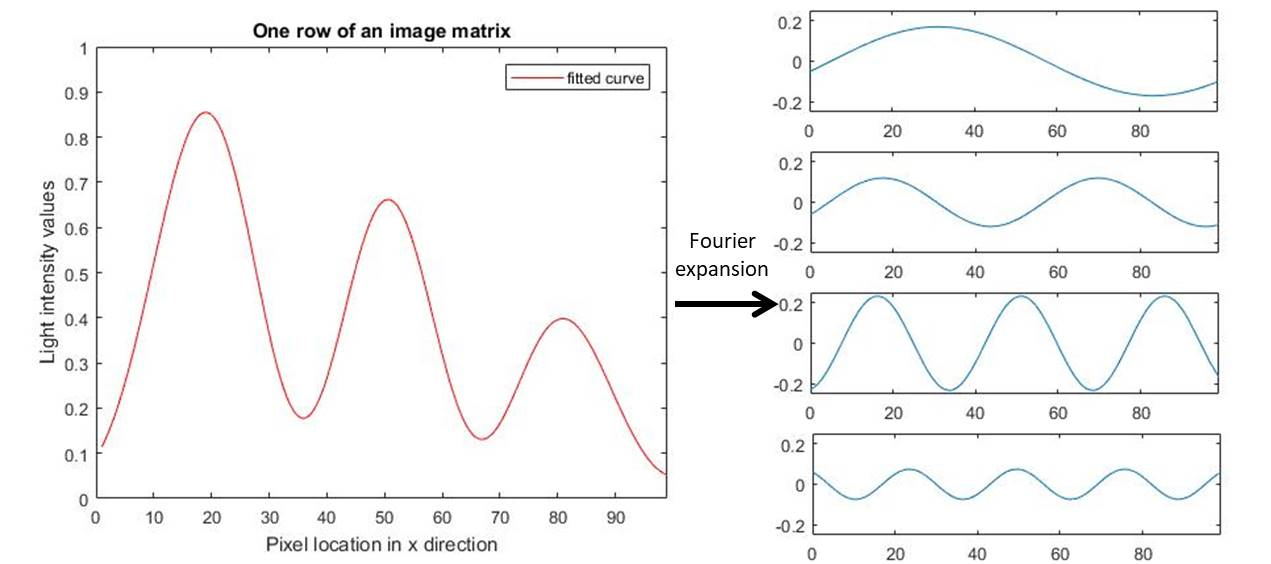
\includegraphics[scale=0.6]{fourier_expansion.jpg}
%     \caption{Example to illustrate the Fourier expansion of a row of an image matrix}
%     \label{fig:fourier}
% \end{figure}

% Using Fourier series expansion this function can be broken down into a series of sine and cosine functions with each sine-cosine function pair having a unique frequency referred to as a spatial frequency. The sine-cosine functions of different spatial frequencies can be seen on the right in Figure \ref{fig:fourier}. Therefore an image can be broken down into sine-cosine functions of different frequencies in the same way as a temporal function with the difference being that the image contains spatial frequencies as opposed to temporal frequencies \cite{bourne2010spatial}. Therefore, since images can be broken down into a series of sine-cosine functions, images can be taken from the spatial domain to the frequency domain by using the Fast Fourier Transform algorithm (FFT).

% In order to perform correlation in the frequency domain the correlation equation must be related to an equivalent function in the frequency domain. This is done using the cross correlation equation. Cross correlation is a method used to determine the similarity between two signals as a function of the displacement or lag of the one relative to the other. In the continuous case the cross correlation between continuous functions $f$ and $g$ is 
% \begin{equation}
% \label{eq: cross correlation cont}
%  (f\otimes g)(t) \triangleq \int_{-\infty}^{\infty} f^*(\tau) g(\tau+t) \mathrm{d} \tau
% \end{equation}
% where $t$ is known as the lag between the two signals and $f^*$ denotes the complex conjugate of $f$. It is important to note that the resulting function gives the cross-correlation value between the signals as a function of the lag $t$. Similarly an operation known as convolution is defined as
% \begin{equation}
%   (f * g)(t) \triangleq \int_{-\infty}^{\infty} f(\tau) g(t-\tau) \mathrm{d} \tau.
% \end{equation}

% It can be proved that cross correlation and convolution are related by the following equation.
% \begin{equation}
%   (f(\tau) \otimes g(\tau))(t) = (f^*(-\tau) * g(\tau))(t)
% \end{equation}
% The reason for calculating cross correlation by using convolution is so that the convolution theorem can be used. The convolution theorem states that convolution in the time or spatial domain is equivalent to multiplication in the frequency domain. More specifically the Fourier Transform of a convolution is equivalent to the product of the Fourier Transforms of the functions which are being convoluted. This is expressed mathematically as
% \begin{equation}
% \label{eq: convolution theorem}
%   \mathcal{F} \left[ (f(\tau) * g(\tau))(t) \right] = \mathcal{F} \left[ f(\tau) \right] \times \mathcal{F} \left[ g(\tau) \right]
% \end{equation}
% where $\mathcal{F}$ denotes the Fourier Transform operation. Note that the multiplication in this equation is element wise multiplication. This greatly improves the efficiency of convolution \todo{explain why}. Using equations \ref{eq: cross correlation cont} thorough \ref{eq: convolution theorem} correlation is performed in the frequency domain according to
% \begin{equation}
%   (f \otimes g)(t) = (f^*(-\tau) * g(\tau))(t) = \mathcal{F}^{-1} \left[ \mathcal{F} \left[ f^*(\tau) \right] \times \mathcal{F} \left[ g(\tau) \right] \right]
% \end{equation}
% where $\mathcal{F}^{-1}$ is the inverse Fourier Transform. Note that $f^*(-\tau)$ changed to $f^*(\tau)$ within the Fourier Transform in accordance with the complex conjugation property of the Fourier Transform \cite{arfken2011mathematical}. The mathematics presented here is for a one-dimensional, continuous function however the relations hold for the case of two-dimensional, discrete functions such as images.

% The discrete Fourier Transform of an image matrix is determined according to
% \begin{equation}
%   \mathcal{F} \left[ F(x,y) \right] = \mathbf{F}(u,v) = \sum_{x=0}^{x=M-1} \sum_{y=0}^{y=N-1} F(x,y) e^{-i2\pi(\frac{xu}{M}+\frac{yv}{N})}
% \end{equation}
% where $i$ is the imaginary number and $M$ and $N$ are the number of pixels within the image in the x and y directions respectively. Here $u=0,1,2,...M-1$ and $v=0,1,2,...N-1$ in order to fully populate the discrete Fourier Transform matrix ,$\mathbf{F}(u,v)$, of the image.

% Phase shift correlation relies upon using the assumption that the deformed image, $G$, is equivalent to the reference image, $F$, shifted in the x and y direction by $\Delta x$ and $\Delta y$ respectively \cite{barros2017dft}.
% \begin{equation}
%   G(x,y)=F(x + \Delta x, y + \Delta y)
% \end{equation}
% Therefore the Discrete Fourier Transform of the deformed image can be expressed as
% \begin{align}
%    \mathcal{F} \left[ G(x,y) \right] &= \mathcal{F} \left[ F(x + \Delta x,y + \Delta y) \right] \\ &=  \sum_{x=0}^{x=M-1} \sum_{y=0}^{y=N-1} F(x + \Delta x,y + \Delta y) e^{-i2\pi(\frac{xu}{M}+\frac{yv}{N})} \\
%    \text{letting} \quad &x'=x+\Delta x \quad \text{and} \quad y'=y+\Delta y \\
%    &=  \sum_{x'=0}^{x'=M-1} \sum_{y'=0}^{y'=N-1} F(x',y') e^{-i2\pi(\frac{(x'-\Delta x)u}{M}+\frac{(y'-\Delta y)v}{N})} \\
%    &=  e^{-i2\pi(\frac{-\Delta x u}{M}+\frac{-\Delta y v}{N})} \sum_{x'=0}^{x'=M-1} \sum_{y'=0}^{y'=N-1} F(x',y') e^{-i2\pi(\frac{x'u}{M}+\frac{y'v}{N})} \\
%    &=  \mathcal{F} \left[ F(x,y) \right] e^{i2\pi(\frac{\Delta x u}{M}+\frac{\Delta y v}{N})} .
% \end{align}

% Thus the correlation between image matrices $F(x,y)$ and $G(x,y)$ is calculated as
% \begin{align}
%   (F(x,y) \otimes G(x,y))(l,k) &= \mathcal{F}^{-1} \left[ \mathcal{F} [F^*(x,y)] \times \mathcal{F} [G(x,y)] \right] \\
%   &= \mathcal{F}^{-1} \left[ \mathcal{F} [F^*(x,y)] \times \mathcal{F} \left[ F(x,y) \right] \times e^{i2\pi(\frac{\Delta x u}{M}+\frac{\Delta y v}{N})} \right] \\
%   &= \mathcal{F}^{-1} \left[ \mathbf{F}^*(u,v) \times \mathbf{F}(u,v) \times e^{i2\pi(\frac{\Delta x u}{M}+\frac{\Delta y v}{N})} \right] \\
%   &= \mathcal{F}^{-1} \left[ \left| \mathbf{F}(u,v) \right|^2 \times e^{i2\pi(\frac{\Delta x u}{M}+\frac{\Delta y v}{N})} \right] \label{eq: FFT impulse}
% \end{align}
% which returns a matrix where the each element of the matrix is a cross-correlation value for the two image matrices where image $G(x,y)$ has been shifted in the x and y direction by a specific amount. The shift of image $G(x,y)$ is related to the index of the matrix. For images of size $M$ by $N$ the indexes $l$ and $k$ correspond to shifting image $G(x,y)$ by $x_{shift}$ and $y_{shift}$, to get $G(x+x_{shift},y+y_{shift})$, according to
% % this equation is for shifting of F not G
% % \begin{align}
% %   x_{shift}&= 
% %     \begin{cases}
% %         l-1 & \text{if $l \leq \frac{M}{2}+1$ and M is even} \\
% %         l-2-M & \text{if $l > \frac{M}{2}+1$ and M is even}   \\
% %         l-1 & \text{if $l \leq \frac{M+1}{2}$ and M is odd} \\
% %         l-2-M & \text{if $l > \frac{M+1}{2}$ and M is odd}
% %     \end{cases} \\
% %   y_{shift}&= 
% %     \begin{cases}
% %         k-1 & \text{if $k \leq \frac{N}{2}+1$ and N is even} \\
% %         k-2-N & \text{if $k > \frac{N}{2}+1$ and N is even}   \\
% %         k-1 & \text{if $k \leq \frac{N+1}{2}$ and N is odd} \\
% %         k-2-N & \text{if $k > \frac{N+1}{2}$ and N is odd}
% %     \end{cases}
% % \end{align}

% \begin{align}
%   x_{shift}&= 
%     \begin{cases}
%         1-l & \text{if $l \leq \frac{M}{2}+1$ and M is even} \\
%         M+2-l & \text{if $l > \frac{M}{2}+1$ and M is even}   \\
%         1-l & \text{if $l \leq \frac{M+1}{2}$ and M is odd} \\
%         M+2-l & \text{if $l > \frac{M+1}{2}$ and M is odd}
%     \end{cases} \label{eq: FFT xshift} \\
%   y_{shift}&= 
%     \begin{cases}
%         1-k & \text{if $k \leq \frac{N}{2}+1$ and N is even} \\
%         N+2-k & \text{if $k > \frac{N}{2}+1$ and N is even}   \\
%         1-k & \text{if $k \leq \frac{N+1}{2}$ and N is odd} \\
%         N+2-k & \text{if $k > \frac{N+1}{2}$ and N is odd}
%     \end{cases} \label{eq: FFT yshift}
% \end{align}

% Referring back to equation \ref{eq: FFT impulse} the term $e^{i2\pi(\frac{\Delta x u}{M}+\frac{\Delta y v}{N})}$ is a Fourier Transform of a finite response impulse function which has its peak located at $(\Delta x, \Delta y)$ in the spatial domain. Therefore when computing the cross-correlation between two images using the FFT method described above the resulting matrix contains correlation values for various shifts applied to image $G(x,y)$ and the highest correlation value occurs at point $(\Delta x, \Delta y)$ corresponding to the optimal shifting of the deformed image to bring it into alignment with the reference image. These index values $\Delta x$ and $\Delta y$ are substituted into Equations \ref{eq: FFT xshift} and \ref{eq: FFT yshift} respectively to determine the optimal shift that should be applied to the deformed image.

% Although this method of correlation is substantially faster than either Newton-Raphson or Lucas-Kanade, especially as the subset size increases, it has limitations. First of all only shifts of integer values can be investigated since this method does not employ interpolation. This limitation can be overcome by modifying the method to perform interpolation to increase the resolution of the matrices in the frequency domain \cite{malah1976dft}. However, in this project, the FFT based correlation is intended to be used to determine an initial guess for the Newton-Raphson and Lucas-Kanade algorithms so sub-pixel correlation is not important.

% The second limitation is that this method can only determine the optimal shift values if they are less than half the size of the subset. This is of little concern since subset size can simply be adjusted to compensate for this if the need arises.

% % Cross power spectral density
% % This (say that it is based on the phase shift theorem and reference paper)
% % Cross correlation is performed by using convolution so that the 
% % explain FFT and why faster
% % relate cross cor to convolution and convolution to FFT

% \section{Subset splitting}
% One of the major downfalls of DIC is that it assumes that the deformation field over every subset is continuous. Although this is true most of the time it breaks down when there is a displacement discontinuity in the specimen resulting from the presence of cracks or shear bands. In order to deal with this issue the method of subset splitting proposed by Poissant and Barthelat \cite{poissant2010novel} was implemented. In this method an equation defining a line, that passes through the subset, is used to split the pixels within the subset into two groups and a different set of warp function parameters is used for each group. Thus if the line is placed such that it lies on the crack the subset will be split into two groups allowing the deformations on either side of the crack to be determined separately. 

% The first step is to determine the equation for the line such that it lies on the crack. A straight line is used to approximate the crack since a curve would make the process more complex and is in general not necessary since the subsets only capture a small portion of the crack. The method proposed by Poissant and Barthelat \cite{poissant2010novel} for determining the this line was found to give inconsistent results. Instead a more robust method, although more computationally expensive, was implemented in the form of a particle swarm. The equation for the line is of the form 
% \begin{align}
%     y&=m \times (x-d) + c \\
%     \text{where} \quad m&=\tan{\theta}
% \end{align}
% where $d$ is the shift in the x direction, $c$ is the shift in the y direction and $m$ is the gradient which corresponds with angle $\theta$. The reason for including a shift in both directions is so that a definitive bounds can be placed on the range of values evaluated by the particle swarm algorithm. In other words if the shift in the x direction $d$ was taken out of the equation then the shift in the y direction $c$ would have to range from negative infinity to infinity in order to compensate. The x and y direction shifts are evaluated from zero to the subset size and the angle $\theta$ is evaluated from $0^\circ$ to $180^\circ$ measured anti-clockwise from the x-axis. 

% Particle swarm optimisation is performed using the correlation coefficient equation as the objective function. This correlation coefficient equation takes in two sets of warp function parameters and the line equation for the crack. It then splits the pixels in the subset into the two groups according to the line equation for the crack and warps each group of pixels according to their set of warp function parameters. Then interpolation is performed on all the pixels in the subset and the chosen correlation equation is used to determine the degree of fit. Note that the particle swarm algorithm only investigates the three parameters $d$, $c$ and $\theta$ but the algorithm requires the two sets of warp function parameters to be provided.

% These two sets of warp function parameters are taken as the warp function parameters of two subsets, with good correlation coefficient values, nearest to the subset under consideration. A temporary line is drawn through the centre of the subset under consideration such that this line has a gradient that is perpendicular to the line for the crack. Then the subset whose warp function parameters are to be used as an input for the particle swarm algorithm is the one which is nearest to the subset under consideration, has a good correlation value and is intersected by this temporary line. Such a subset is found on both sides of the crack line so that there is an appropriate guess of the warp function parameters for both groups of pixels.

% The second step is to perform correlation on the subset according to the splitting line. To do this the Lucas-Kanade and Newton-Raphson algorithms discussed earlier need to be modified slightly. The subset is split up into two groups with each group having its own set of warp function parameters to optimise. Therefore within each algorithm the line equation is used to split the pixels within the subsets into these two groups. Then for the Newton-Raphson algorithm a Jacobian and Hessian is computed for each group of pixels. This is done by evaluating Equations \ref{eq: jacobian hand} and \ref{eq: hessian hand} using only the pixels within the group under consideration. With the Jacobian and Hessian known for each group the warp function parameters of both groups can be updated by computing the update for each group separately using Equation \ref{eq: Newton update}.

% Similarly for the Lucas-Kanade algorithm the RHS term of Equation \ref{eq:delta p} is evaluated separately for both groups of pixels and the warp function parameters for each group are updated separately using Equation \ref{eq: LK update}. Although the warp function parameters are updated separately in both algorithms, the correlation coefficient is determined for the whole subset using both groups of pixels. This is because the correlation coefficient needs to indicate the degree of fit for a specific line equation and two sets of warp function parameters.

% Once the subset has been successfully correlated using the subset-splitting method there are two sets of warp function parameters but only one set can be recorded per subset. The set of warp function parameters that applies to the largest number of pixels in the subset is recorded for the subset since this set of warp function parameters plays the larger role with respect to the correlation coefficient. In other words there is more material on this side of the crack line, within the subset, associated with this set of warp function parameters.

% how works for diff algorithms
% finding crack orientation
% initial guess


% \section{Stopping criteria}
% The subset matching algorithm will continue to improve the warp function parameters until stopped. Thus a means of determining when the iterations should stop is needed. Ideally the iterations should stop once the correlation between the subsets is sufficiently accurate. Thus correlation could be halted once the correlation criteria coefficient has reached the desired value. However determining the correlation coefficient within each iteration is computationally expensive. Therefore the stopping criteria suggested by B. Pan \cite{panfast} is used since it is much more efficient to compute. This criteria halts the iterations once the norm of the warp function parameter update is less than $0.001$.
% \begin{align}
%   ||\Delta \bm{p}|| &= \sqrt{(\Delta u)^2 + (\Delta \tilde{x}\times\Delta \frac{\partial u}{\partial x}) + (\Delta \tilde{y}\times \Delta \frac{\partial u}{\partial y}) + (\Delta v)^2 + (\Delta \tilde{x}\times\Delta \frac{\partial v}{\partial x}) + (\Delta \tilde{y}\times \Delta \frac{\partial v}{\partial y})} \nonumber \\
%   &\text{where} \quad \Delta \tilde{x} = max(\Delta x) \quad \text{and} \quad \Delta \tilde{y} = max(\Delta y)
% \end{align}

% \section{Algorithm outline}
% The steps performed within the algorithm in order to achieve correlation are listed here in order to illustrate how the theory presented here is related to the code. It should be noted that the initial guesses for the warp function parameters were determined by the user selecting seed points in the reference and investigated images.

% \subsection{Lucas-Kanade}
% The following is the steps executed within the Lucas-Kanade subset matching method.
% \begin{enumerate}
%   \item First $\mean{F}$ is determined for the reference subset.
%   \item Then $\triangledown F$ is calculated using Matlab's built in image gradient function (imgradientxy) and the Jacobian of the warp function is calculated. These are then used to determine the Hessian matrix.
%   \item Thereafter $\Delta F$ is determined since it too remains constant.
%   \item The initial guess for the warp function parameters is then used to calculate the $\Delta x_{warp}$ and $\Delta y_{warp}$ for the investigated subset $G$ using equation \ref{eq:warp}.
%   \item $\Delta x_{warp}$ and $\Delta y_{warp}$ are used in equation \ref{eq:subset warp} to obtain the warped version of the investigated subset.
%   \item $\mean{G}$ and $\Delta G$ are then determined.
%   \item With all the necessary values determined; equation \ref{eq:delta p} can be used to calculate $\Delta \bm{p}$.
%   \item Then equation \ref{eq:get new p} is used to determine the updated approximation to the warp function parameters.
%   \item Step 4 until step 8 are repeated until the stopping criteria is satisfied.
% \end{enumerate}

% \subsection{Newton-Raphson}
% The following illustrates the steps executed during the Newton-Raphson subset matching method.
% \begin{enumerate}
%   \item First the bicubic interpolation coefficients are determined for the deformed subset.
%   \item Then the Jacobian and Hessian are determined for the current estimate of the warp function parameters.
%   \item Use the Jacobian and Hessian to calculate the search direction.
%   \item Thereafter golden section search method is used to determine the optimal step size for the search direction.
%   \item Determine the norm of the change in the warp function parameters. If it is smaller than a predefined amount then correlation has been achieved otherwise repeat steps 2 until 5.
% \end{enumerate}

% \chapter{Code explanation}
% \section{interpolation}
% It is clear that warping a subset according to equation \ref{eq:subset warp} requires that the light intensity values between pixel locations can be determined. This is an issue because images store this information in a discrete manner. This is solved by using interpolation to determine the light intensity values between pixels based on the light intensity values of neighbouring pixels. For the purposes of this project Matlab's built in interp2 fucntion was used to perform linear interpolation to determine the light intensity values for non-standard pixel locations where needed.




% Image interpolation is typically the most time consuming part of the correlation process for iterative sub-pixel DIC algorithms \cite{pan2016performance}. Therefore the interpolation schemes have been implemented in the most efficient way for the respective correlation algorithms.

% The two different correlation algorithms used require different information from the interpolation scheme. The Lucas-Kanade algorithm only needs the interpolated light intensity values at the query points. Newton-Raphson on the other hand also needs the interpolation coefficients since the Hessian matrix is dependent on these interpolation coefficients. As such two different interpolation schemes have been used in these correlation algorithms.

% Although these interpolation schemes are different they are both based on bicubic interpolation which attempts to fit a 4th order, two-dimensional polynomial surface to the known light intensity values at integer pixel locations. Thus a query point will lie within a square which has integer pixel locations at the corners of the square. The x and y coordinates of the query point are substituted into the equation for the surface to interpolate the approximate light intensity value. Each square section between integer pixel locations has its own equation making this interpolation piecewise.

% A 4th order, two-dimensional polynomial surface has 16 coefficients which define the surface. As such 16 integer pixel points are required to determine these 16 coefficients. Therefore a $4 \times 4$ submatrix of light intensity values is required to determine the polynomial surface that approximates the light intensity values between the 4 integer pixel locations at the centre of the submatrix.


% \subsection{Lucas-Kanade}
% The Lucas-Kanade algorithm uses a matlab interpolation function called "griddedInterpolant" with the bicubic convolution based interpolation option selected. This function was chosen since it performs interpolation once, before starting the iterations, to create an interpolant object and this interpolant object is then called, within the iterations, to perform fast interpolation at the query points.

% \subsection{Newton-Raphson}
% Although "griddedInterpolant" works well for the Lucas-Kanade algorithm it doesn't not return the coefficients of interpolation. Therefore a function was created to solve for the coefficients of interpolation by fitting the 4th order, two-dimensional polynomial surface to a $4 \times 4$ submatrix of the image. This method of bicubic interpolation is rather basic but it still works well.

% First consider the equation of the surface that is to be fitted
% \begin{equation}
%   F(x,y)=\sum^4_{i=1} \sum^4_{j=1} a_{ij} \times x^{i-1} y^{j-1}
% \end{equation}
% where $a_{ij}$ are the coefficients of the interpolation equation. Here x and y are the fractional parts of the pixel positions; thus they fall between zero and one.

% To solve for the coefficients we need to calculate the gradients of the polynomial function at the four centre integer pixel locations. This is done using numerical differentiation techniques; specifically the two-point central difference formula. For the three partial derivatives these formulas are \cite{gilat2004matlab}
% \begin{align}
%   \frac{\partial F(x_i,y_j)}{\partial x} &= \frac{F(x_{i+1},y_j)-F(x_{i-1},y_j)}{2} \\
%   \frac{\partial F(x_i,y_j)}{\partial y} &= \frac{F(x_{i},y_{j+1})-F(x_{i},y_{j-1})}{2} \\
%   \frac{\partial^2 F(x_i,y_j)}{\partial x \partial y} &= \frac{\left[ F(x_{i+1},y_{j+1})-F(x_{i-1},y_{j+1}) \right] - \left[ F(x_{i+1},y_{j-1})-F(x_{i-1},y_{j-1}) \right]}{4}.
% \end{align}
% Note that since the x and y coordinates are integers the function values at these points correspond to the light intensity values at integer pixel locations which are known. Therefore these gradients can be solved immediately. Once this is done there are 12 gradients that are known and 4 integer pixel light intensity values. Thus these 16 known values can be used to solve for the 16 coefficients of the polynomial equation. The equations to do this are obtained by substituting the four centre integer pixel location x and y values ((0,0), (0,1), (1,0) and (1,1)) into the polynomial equation, the x partial derivative of the polynomial equation, the y partial derivative of the polynomial equation and the x-y partial derivative of the polynomial equation. This results in 16 equation with the known pixel light intensity values and the known gradients as a function of the coefficient of the polynomial equation. However by substituting the symbolic expression for the gradients and the integer pixel light intensity values the equations can be solved simultaneously to give the coefficients as a function of the known integer pixel light intensity values. These equations are then
% \begin{align}
%   A_{11} &= F(x_2,y_2) \\
%   A_{12} &= -0.5 \times F(x_2,y_1) + 0.5 \times F(x_2,y_3) \\
%   A_{13} &= F(x_2,y_1) - 2.5 \times F(x_2,y_2) + 2 \times F(x_2,y_3) - 0.5 \times F(x_2,y_4) \\
%   A_{14} &= -0.5 \times F(x_2,y_1) + 1.5 \times F(x_2,y_2) - 1.5 \times F(x_2,y_3) + 0.5 \times F(x_2,y_4) \\
%   A_{21} &= -0.5 \times F(x_1,y_2) + 0.5 \times F(x_3,y_2) \\
%   A_{22} &= 0.25 \times F(x_1,y_1) - 0.25 \times F(x_1,y_3) - 0.25 \times F(x_3,y_1) + 025 \times F(x_3,y_3) \\
%   % \begin{split}
%   A_{23} &= -0.5 \times F(x_1,y_1) + 1.25 \times F(x_1,y_2) - F(x_1,y_3) + 0.25 \times F(x_1,y_4) \nonumber \\ &+ 0.5 \times F(x_3,y_1) - 1.25 \times F(x_3,y_2) + F(x_3,y_3) - 0.25 \times F(x_3,y_4) \\
%   % \end{split} \\
%   A_{24} &= 0.25 \times F(x_1,y_1) - 0.75 \times F(x_1,y_2) + 0.75 \times F(x_1,y_3) - 0.25 \times F(x_1,y_4) \nonumber \\ &- 0.25 \times F(x_3,y_1) + 0.75 \times F(x_3,y_2) - 0.75 \times F(x_3,y_3) + 0.25 \times F(x_3,y_4) \\
%   A_{31} &= F(x_1,y_2) - 2.5 \times F(x_2,y_2) + 2 \times F(x_3,y_2) - 0.5 \times F(x_4,y_2) \\
%   A_{32} &= -0.5 \times F(x_1,y_1) + 0.5 \times F(x_1,y_3) + 1.25 \times F(x_2,y_1) - 1.25 \times F(x_2,y_3) \nonumber \\ &- F(x_3,y_1) + F(x_3,y_3) + 0.25 \times F(x_4,y_1) - 0.25 \times F(x_4,y_3) \\
%   A_{33} &= F(x_1,y_1) - 2.5 \times F(x_1,y_2) + 2 \times F(x_1,y_3) - 0.5 \times F(x_1,y_4) \nonumber \\ &- 2.5 \times F(x_2,y_1) + 6.25 \times F(x_2,y_2) - 5 \times F(x_2,y_3) + 1.25 \times F(x_2,y_4) \nonumber \\ &+ 2 \times F(x_3,y_1) - 5 \times F(x_3,y_2) + 4 \times F(x_3,y_3) - F(x_3,y_4) - 0.5 \times F(x_4,y_1) \nonumber \\ &+ 1.25 \times F(x_4,y_2) - F(x_4,y_3) + 0.25 \times F(x_4,y_4) \\
%   A_{34} &= -0.5 \times F(x_1,y_1) + 1.5 \times F(x_1,y_2) - 1.5 \times F(x_1,y_3) + 0.5 \times F(x_1,y_4) \nonumber \\ &+ 1.25 \times F(x_2,y_1) - 3.75 \times F(x_2,y_2) + 3.75 \times F(x_2,y_3) - 1.25 \times F(x_2,y_4) \nonumber \\ &- F(x_3,y_1) + 3 \times F(x_3,y_2) - 3 \times F(x_3,y_3) + F(x_3,y_4) + 0.25 \times F(x_4,y_1) \nonumber \\ &- 0.75 \times F(x_4,y_2) + 0.75 \times F(x_4,y_3) - 0.25 \times F(x_4,y_4) \\
%   A_{41} &= -0.5 \times F(x_1,y_2) + 1.5 \times F(x_2,y_2) - 1.5 \times F(x_3,y_2) + 0.5 \times F(x_4,y_2) \\
%   A_{42} &= 0.25 \times F(x_1,y_1) - 0.25 \times F(x_1,y_3) - 0.75 \times F(x_2,y_1) + 0.75 \times F(x_2,y_3) \nonumber \\ &+ 0.75 \times F(x_3,y_1) - 0.75 \times F(x_3,y_3) - 0.25 \times F(x_4,y_1) + 0.25 \times F(x_4,y_3) \\
%   A_{43} &= -0.5 \times F(x_1,y_1) + 1.25 \times F(x_1,y_2) - F(x_1,y_3) + 0.25 \times F(x_1,y_4) \nonumber \\ &+ 1.5 \times F(x_2,y_1) - 3.75 \times F(x_2,y_2) + 3 \times F(x_2,y_3) - 0.75 \times F(x_2,y_4) \nonumber \\ &- 1.5 \times F(x_3,y_1) + 3.75 \times F(x_3,y_2) - 3 \times F(x_3,y_3) + 0.75 \times F(x_3,y_4) \nonumber \\ &+ 0.5 \times F(x_4,y_1) - 1.25 \times F(x_4,y_2) + F(x_4,y_3) - 0.25 \times F(x_4,y_4) \\
%   A_{44} &= 0.25 \times F(x_1,y_1) - 0.75 \times F(x_1,y_2) + 0.75 \times F(x_1,y_3) - 0.25 \times F(x_1,y_4) \nonumber \\ &- 0.75 \times F(x_2,y_1) + 2.25 \times F(x_2,y_2) - 2.25 \times F(x_2,y_3) + 0.75 \times F(x_2,y_4) \nonumber \\ &+ 0.75 \times F(x_3,y_1) - 2.25 \times F(x_3,y_2) + 2.25 \times F(x_3,y_3) - 0.75 \times F(x_3,y_4) \nonumber \\ & - 0.25 \times F(x_4,y_1) + 0.75 \times F(x_4,y_2) - 0.75 \times F(x_4,y_3) + 0.25 \times F(x_4,y_4)
% \end{align}
% Thus the coefficients of interpolation are determined by substituting in the known integer pixel light intensity values into the above equations.

% Interpolation is carried out over the whole image prior to the correlation process. Once the coefficients have been determined they are stored in ".mat" file. Then when interpolation needs to be performed within the correlation process the required coefficients are loaded from the saved file use Matlabs "matfile" function. This function is used since it enables the algorithm to only load the required coefficients thereby reducing the memory used. This is important since the Newton-Raphson algorithm needs a substantial amount of memory when correlation is done using parallel computing. This method of saving the coefficient for later use is common for interpolation schemes of this type.


%end big commenting
















% \subsection{Speckle pattern generator}
% It was discovered that because creating synthetic images involves a large number of simple operations it would run much faster on a graphics processing unit (GPU). In order to do this the equation \ref{eq: speckle} had to be vectorized \todo{not sure this word is 100\% accurate} so that the light intensities at many points in the image could be evaluated simultaneously using matrix multiplication. 

% First the function creates a grid of points (X and Y) that correspond to the centre location of the pixels which are to be generated. However a jittered grid of points is required for each pixel for the purposes of jittered super sampling. These points are obtained by displacing the pixel centre location, many times, to obtain a jittered grid of points that fall within the fillfactor area of the pixel. The same displacements are applied to each pixel centre location to create its corresponding jittered grid. Since multiple points are created for each pixel, the pixel locations are reshaped into a column vector (line 13 and 14) and the displacements are added as row vectors resulting in a matrix where each row holds the super sampling locations for each pixel. 

% The row vector of displacement values are created in 3 steps. First the grid-spacing between the points of the unjittered grid are determined in both directions (xdist and ydist) based on the step size between pixels (stepsize), the fill factor (fillfactor) and the number of points in each direction of the grid (numpoints). The second step uses these grid-spacings to determine the x and y displacements of the unjittered grid (xgrid1 and ygrid1). These are then used to create 2 matrices of unjittered displacement values for the x and y direction (xgrid2 and ygrid2). 

% The final step involves jittering the displacement values. This is done by creating a 2 matrices of random values between -0.5 and 0.5, multiplying them by their corresponding grid-spacing and adding them to the matrices of unjittered displacement values to get the two final matrices of jittered displacement values (xgrid3 and ygrid3 at line 32). These matrices are then reshaped to be row vectors (xxgrid and yygrid) which are passed to the GPU to be stored in VRAM (Video Random Access Memory).

% Thereafter the function defines the speckle pattern by assigning values to the properties of each speckle. First the vector of speckle sizes is converted from units of pixels to the units used in the displacement function hereafter referred to as displacement units (line 40). It was originally in units of pixels because for a good image the speckle sizes must be proportional to the subset size which is in units of pixels. The position of the speckles are then defined ,in displacement units, at random locations that fall within the range of the image. The light intensity at the centre of each speckle is then randomly defined to fall in the range between 0.5 and 1 where 1 is white and 0 is black.

% The choice to alter the speckle radius in a sinusoidal manner lead to some issues when the frequency of the sinusoid increased. At higher frequencies the resulting speckle would represent a star shape which is an unrealistic speckle shape. In order to adjust for this the amplitude of the sinusoid was adjusted based on its frequency using the function defined on line 48. This function exponentially decreases the amplitude of the sinusoid as the frequency increases.

% The for loop starting at line 54 saves the details of every speckle. First a random phase shift (a) and frequency (b) are defined. The amplitude (c) is then determined based on the frequency using the function on line 48. The base radius (d), x and y positions (Xk and Yk) and the light intensity (I0) are then all saved.

% GPUs have a limited amount of VRAM and so the number of points that can be evaluated at once is limited. To cope with this the points to be evaluated are divided into groups so that the VRAM required to evaluate each group is less than what is available. The number of groups is determined by dividing the overall memory requirements of the total image by the memory that is available. Using a simplified approach the total memory requirements of the image is the number of pixels in the image times the number of points that need to be evaluated for each pixel times the number of speckles. This is divided by the available memory which is 44567000 for the computer used during this project. If a different computer is used this value should be adjusted. Note that these memory values are relative values and have no units.

% Super sampling relies upon using the average of the sampled locations for each pixel to determine that pixels light intensity value. A Gaussian weighted average (H at line 72) is used to do this in order to allow the sampled locations closer to the pixel centre to have a greater influence on the light intensity value. The weighted average matrix is reshaped into a row vector and then this row vector is repeated to form a matrix (HH). The number of rows in this matrix is equivalent to the number of pixels that are evaluated on each pass to the GPU.

% With all the necessary variables defined the calculation of light intensity values at specific locations in the image can commence. This is done between lines 79 and 154. A counter is used to keep track of which group of elements is to be processed. The variables "begin" and "ending" correspond to the indexes of the first and last elements in X and Y that are to be to be processed (which pixels are to be processed) while "ending2" gives the number of pixels to be computed in each pass to the GPU ("ending2" is equal to "numOfPixels" except on the last pass to the GPU where a smaller number of pixels is processed)

% For the reference image (imageCount=1) the points to be evaluated (Xin and Yin) are determined by adding the row vectors of jittered displacements (xxgrid and yygrid) to the column vectors of x and y positions (X and Y). Note that since "X" and "Y" are column vectors with "numOfPixels" amount of rows and "xxgrid" and "yygrid" are row vectors with "numpoints" squared amount of columns the resulting matrices (Xin and Yin) are of size "numOfPixels" by "numpoints" squared. Each row in "Xin" and "Yin" is a collection of the jittered super sampling positions for a single pixel. Therefore each row corresponds to a pixel.

% For the case of the deformed image the points to be evaluated are determined by subtracting the displacement at that point (fux and fuy functions) from the group of x and y positions (X and Y) and then adding the jittered displacement matrices (xxgrid and yygrid). In doing so the pixel point is displaced in the opposite direction compared to what is described by the displacement function. This is done because displacement of the speckle pattern according the the displacement function while holding the pixel locations constant is equivalent to displacing the pixel locations in the opposite direction to the displacement function and holding the speckle pattern constant. 

% At this point the locations at which to evaluated the speckle pattern are available. To evaluate the light intensity at a location in the image involves four steps. The steps will be explained in terms of determining the light intensity at a single location although the algorithm determines this at multiple locations simultaneously. In the first step the distances between all the speckle centres and the location needs to be determined. To do this "Xin" and "Yin" are then reshaped to be column vectors (Xgrid and Ygrid) and the row vectors containing the location of the speckle centres (Xk and Yk) are subtracted from these to give "X1" and "Y1". Each row of "X1" and "Y1" contains the distance between each speckle centre and the specific location in the image.

% The second step involves determining the angles between the imaginary lines, that pass through the speckle centres and the location under consideration, and the x-axis. This is done by applying Matlab's atan2 function to the x and y distances "X1" and "Y1". The third step involves determining the radius of the each speckle along the imaginary line. This is done by applying the phase shifts and frequency changes to the angles, taking the sin of the angles, multiplying them by their respective amplitudes and adding the base radii. This results in the matrix "sins1". Each row of "sins1" gives the radii of the all the speckles in the direction of the location under consideration.

% The fourth step requires determining how much each speckle contributes to the location under consideration. This is done by first determining the squared distance between the speckle centre and the location under consideration which is done using Pythagoras to get "M". The contribution of each speckle is determined by taking the exponent of the negative of this distance (M) divided by the speckle radius squared. This results in the matrix "speckleContribution". 

% Each row in "speckleContribution" gives the contribution of each speckle to the point under consideration. This matrix is then multiplied by the column vector of the speckle light intensities to give a column vector of the overall light intensity at each location under consideration. This row vector is then reshaped to a matrix such that each row contains the light intensities at the jittered super sampling locations for a pixel. Then it is multiplied by the matrix of weighted averages and each row is summed to give a column vector of pixel light intensities. Throughout this process variables are cleared once they are no longer needed in order to free up space on the VRAM.

% Finally these values are collected from the GPU and stored in a column vector on the CPU. Once this vector is fully populated it is reshaped to the size of the desired image and the light intensity values are quantized using Matlab's "imquantize" function. This is 12 bit quantization which is consistent with the quantization that takes place within the camera used for experiments.

% \lstinputlisting[language=Matlab]{analyticalspeckleContinuous7_simplified_for_explanation.m}

% It was discovered that because creating synthetic images involves a large number of simple operations it would run much faster on a graphics processing unit (GPU). In order to to this the equation \ref{eq: speckle} had to be vectorized \todo{not sure this word is 100\% accurate} so that the light intensities at many points in the image could be evaluated simultaneously using matrix multiplication. 

% First the function creates a grid of points (X and Y) that correspond to the centre of the pixels which are to be generated. This grid of points (in matrix format) is then reshaped into a column vector of points. This is done so that these points can be evaluated simultaneously using a matrix multiplication. Thereafter the vector of speckle sizes is converted from units of pixels to the units used in the displacement function hereafter referred to as displacement units. It was originally in units of pixels because for a good image the speckle size must be proportional to the subset size which is in units of pixels. The position of the speckles are then defined at random locations that fall within the range of the image. Note that these locations are in displacement units. The light intensity at the centre of each speckle is then randomly defined to fall in the range between 0.5 and 1 where 1 is white and 0 is black.

% The choice to alter the speckle radius in a sinusoidal manner lead to some issues when the frequency of the sinusoid increased. At higher frequencies the resulting speckle would represent a star shape which is an unrealistic speckle shape. In order to adjust for this the amplitude of the sinusoid was adjusted based on its frequency using the function defined on line 25. This function exponentially decreases the amplitude of the sinusoid as the frequency increases.

% The for loop starting at line 31 saves the details of every speckle. First a random phase shift (a) and frequency (b) are defined. The amplitude (c) is then determined based on the frequency using the function on line 25. The base radius (d), x and y positions (Xk and Yk) and the light intensity (I0) are then all saved.

% GPUs have a limited amount of VRAM (Video Random Access Memory) and so the number of points that can be evaluated at once is limited. To cope with this the points to be evaluated are divided into groups so that the VRAM required to evaluate each group is less than what is available. The number of groups is determined by dividing the overall memory requirements of the total image by the memory that is available. Using a simplified approach the total memory requirements of the image is the number of pixels in the image times the number of points that need to be evaluated for each pixel (for the purpose of super sampling) times the number of speckles. This is divided by the available memory which is 44567000 for the computer used during this project. If a different computer is used this value should be adjusted. Note that these memory values are relative values and have no units.

% Presently the points to be investigated are defined to be at the centre of the pixel locations. However for the purpose of jittered super sampling many points within a pixel must be investigated to give the overall light intensity of the pixel. This is done by applying matrices of displacement values (xgrid3 and ygrid3), which when added to the pixel centre location, creates a jittered grid of points to be investigated which falls within the fillfactor area of the pixel. In this way the super sampling locations for any pixel can be determined by adding these matrices to the location of the pixel centre. These matrices of displacement values are created in 3 steps.

% First the grid-spacing between the points of the unjittered grid in both directions (xdist and ydist) are determined based on the step size between pixels (stepsize - in displacement units), the fill factor (fillfactor) and the number of points in each direction of the grid (numpoints). The second step uses these grid-spacings to determine the x and y displacements of the unjittered grid (xgrid1 and ygrid1). These are then used to create 2 matrices of unjittered displacement values for the x and y direction (xgrid2 and ygrid2). 

% The final step involves jittering the displacement values. This is done by creating a 2 matrices of random values between -0.5 and 0.5, multiplying them by their corresponding grid-spacing and adding them to the matrices of unjittered displacement values to get the two final matrices of jittered displacement values (xgrid3 and ygrid3).These matrices are then reshaped to be row vectors (xxgrid and yygrid) which are passed to the GPU (stored in VRAM).

% Super sampling relies upon using the average of the sampled locations for each pixel to determine that pixels light intensity value. A Gaussian weighted average (H) is used to do this in order to allow the sampled locations closer to the pixel centre to have a greater influence on the light intensity value. The weighted average matrix is reshaped into a row vector and then this row vector is repeated to form a matrix. The number of rows in this matrix is equivalent to the number of pixels that are evaluated on each pass to the GPU.

% With all the necessary variables defined the calculation of light intensity values at specific locations in the image can commence. This is done between line 82 and 152. A counter is used to keep track of which group of elements is to be processed. The variables "begin" and "ending" correspond to the indexes of the first and last elements in X and Y that are to be to be processed while "ending2" gives the number of elements to be computed in each pass to the GPU. "ending2" is equivalent to "$num_of_elements$" except on the last pass to the GPU where a smaller number of pixels is processed.

% For the reference image ($image_count=1$) the points to be evaluated (Xin and Yin) are determined by adding the jittered displacement matrices (xxgrid and yygrid) to the group of x and y positions (X and Y). Note that since "X" and "Y" are column vectors with "$num_of_elements$" amount of rows and "xxgrid" and "yygrid" are row vectors with "numpoints" squared amount of columns the resulting matrices (Xin and Yin) are of size "$num_of_elements$" by "numpoints" squared. Each row in "Xin" and "Yin" is a collection of the jittered super sampling positions for a single pixel. Therefore each row corresponds to a pixel.

% For the case of the deformed image the points to be evaluated are determined by subtracting the displacement at that point (fux and fuy functions) from the group of x and y positions (X and Y) and then adding the jittered displacement matrices (xxgrid and yygrid). In doing so the pixel point is displaced in the opposite direction compared to what is described by the displacement function. This is done because displacement of the speckle pattern according the the displacement function while holding the pixel locations constant is equivalent to displacing the pixel locations in the opposite direction to the displacement function and holding the speckle pattern constant. 
% %Thus by altering the pixel locations according to the inverse of the displacement function the resulting image exhibits speckle pattern which has moved according to the displacement function.

% At this point the locations at which to evaluated the speckle pattern are available. To evaluate the light intensity at a location in the image involves four steps. The steps will be explained in terms of determining the light intensity at a single location although the algorithm determines this at multiple locations simultaneously. In the first step the distances between all the speckle centres and the location needs to be determined. To do this "Xin" and "Yin" are then reshaped to be column vectors (Xgrid and Ygrid) and the row vectors containing the location of the speckle centres (Xk and Yk) are subtracted from these to give "X1" and "Y1". Each row of "X1" and "Y1" contains the distance between each speckle centre and that specific location in the image.

% The second step involves determining the angles between the imaginary lines, that pass through the speckle centres and the location under consideration, and the x-axis. This is done by applying Matlab's atan2 function to the x and y distances "X1" and "Y1". The third step involves determining the radius of the each speckle along the imaginary line. This is done by applying the phase shifts and frequency changes to the angles, taking the sin of the angles, multiplying them by their respective amplitudes and adding the base radii. This results in the matrix "sins1". Each row of "sins1" gives the values for the radii of the all the speckles in the direction of the location under consideration.

% The fourth step requires determining how much each speckle contributes to the location under consideration. This is done by first determining the squared distance between the speckle centre and the location under consideration which is done using Pythagoras to get "M". The contribution of each speckle is determined by taking the exponent of the negative of this distance (M) divided by the speckle radius. This results in the matrix "temp". Each row in temp gives the contribution of each speckle to the point under consideration. This matrix is then multiplied by the column vector of the speckle light intensities to give a column vector of the overall light intensity at each location under consideration. This row vector is then reshaped to a matrix such that each row contains the light intensities at the jittered super sampling locations for a pixel. Then it is multiplied by the matrix of wieghted averages and each row is summed to give a column vector of pixel light intensities. 

% Finally these values are collected from the GPU and stored in a column vector on the CPU. Once this vector is fully populated it is reshaped to the size of the desired image.




\chapter{Synthetic validation}
\label{ch: synthetic validation}
\hl{Before the DIC framework presented here can be adopted for Materials Engineering purposes it first needs to be validated.} \todo{this should rather refer to the objectives in the intro} Validation requires proving that the performance of the proposed framework is on par with that of commercial software. The commercial software used for comparative purposes is that of LaVision's Davis software.

The accuracy of the displacements computed by DIC is dependent on two aspects: correlation of the images and calibration of the camera system. Correlation deals with computing the displacement fields between images in units of pixels. As such correlation operates solely within the sensor coordinate system. Calibration first determines the parameters of the pinhole camera model for the camera system used and then uses these parameters to relate the displacements in the sensor coordinate system, determined by correlation, to displacements in the world coordinate system. 

Thus the correlation component of the proposed framework can be validated in a standalone manner. However calibration cannot be validated separately from correlation because it operates on the displacements determined from correlation. Therefore validation has been broken up into two parts.

First the correlation framework is validated in this chapter and then the overall DIC framework is validated in the chapter to follow. The proposed correlation framework is validated by showing that the precision and accuracy of its displacement results are on par with that of the Davis software.

% Therefore it is clear that calibration cannot by validated separately from correlation since it is dependent on the displacements determined via correlation. Correlation on the other hand can be validated in a stand-alone manner.

% The proposed DIC framework consists of two parts: correlation and calibration. Ideally these two components would be validated separately in order to validate the overall DIC framework. Although the correlation component can be evaluated in a stand alone manner, the calibration component cannot. This is because validation of the calibration component is not limited to validating the process of determining the calibration parameters but also includes how well these parameters are used to relate displacements in the sensor coordinate system, determined by correlation, to displacements in the world coordinate system. Thus validating the calibration component entails validating the overall DIC framework.

% Therefore validation has been broken up into two parts. First the correlation framework is validated in this chapter and then the overall DIC framework is validated in the chapter to follow. The proposed correlation framework is validated by showing that the precision and accuracy of its displacement results are on par with that of the Davis software.
%The proposed correlation framework is validated by showing that the systematic and random errors of its displacement results are on par with that of the Davis software.

% The proposed correlation framework is validated by showing that the accuracy and precision of its displacement results are on par with that of the Davis software. 

% only working in sensor coordinate system.

\section{Precision and accuracy}
% http://www.webassign.net/question_assets/unccolphysmechl1/measurements/manual.html
% For a measurement method accuracy refers to how close a measured value is to the true value while precision refers to how reproducible this accuracy is. 
% % \todo{is this correct?} Therefore a measurement method needs to be both precise and accurate for it to be valid. Thus the precision and accuracy of the measured displacements need to be quantified to show the validity of the proposed correlation framework.

For a measurement method accuracy refers to how close a measured value is to the true value while precision refers to how reproducible this accuracy is. Precision and accuracy are quantified by the systematic and random errors respectively. For a measurement method the error is defined as the difference between the true value and the measured value. In terms of correlation if the true displacement of subset $i$ in the x and y directions are given as $u_i^{true}$ and $v_i^{true}$ and the measured values are $u_i^{meas}$ and $v_i^{meas}$ then the error in the x and y directions, $\Delta u_i^e$ and $\Delta v_i^e$, are given as
% In terms of correlation if the true displacement of subset $i$ in the x direction is given as $u_i^{true}$ and the measured value is $u_i^{meas}$, measured by performing correlation, then the error, $\Delta u_i^e$, is given as
\begin{equation}
  \label{eq: error}
  \Delta u_i^e = u_i^{meas}-u_i^{true} \quad \text{and} \quad \Delta v_i^e = v_i^{meas}-v_i^{true}.
\end{equation}
% A pair of such errors is associated with the measured displacement of each subset. Therefore when the displacement field between two images has been calculated by performing correlation, which involves many subsets, there is a corresponding group of errors. The systematic and random errors are statistical measurements based on this group of errors. 

A pair of such errors is associated with the measured displacement of each subset. Therefore if $n$ many subsets are used during correlation then there are $n$ many error pairs associated with the calculated displacement field. The systematic and random errors are statistical measurements based on these groups of errors. 

% Therefore if $n$ many subsets are used during correlation to determine the displacement field between two images then there are $n$ many error pairs associated with the displacement field.

% Therefore the displacement field between two images, calculated via correlation, has $n$ many error pairs corresponding to the $n$ subsets used during correlation.

The systematic error is quantified by the mean absolute error in both directions as
\begin{equation}
  \label{eq: mean absolute error}
   \Delta u^{mae} = \frac{\sum_i^n \left| \Delta u_i^e \right| }{n} \quad \text{and} \quad \Delta v^{mae} = \frac{\sum_i^n \left| \Delta v_i^e \right| }{n}.
\end{equation}
The random error is quantified by the standard deviation of the absolute error in both directions given as 
\begin{equation}
  \label{eq: std of abs error}
  \sigma_u = \sqrt{\frac{\sum_i^n \left[ \left| \Delta u_i^e \right| -  \Delta u^{mae} \right]^2}{n-1}} \quad \text{and} \quad \sigma_v = \sqrt{\frac{\sum_i^n \left[ \left| \Delta v_i^e \right| -  \Delta v^{mae} \right]^2}{n-1}}.
\end{equation}
The absolute of the error is used in Equations \ref{eq: mean absolute error} and \ref{eq: std of abs error} so that positive and negative errors do not cancel each other out which would skew the results. Additionally, according to Amiot et al. \cite{amiot2013assessment}, \todo{et al. correct?} to ensure statistical independence in the systematic and random errors it is important that the subsets evaluated do not overlap.

% It is clear that the true displacement of each subset needs to be known in order to evaluated Equations \ref{eq: error}, \ref{eq: mean absolute error} and \ref{eq: std of abs error}. This is not possible for images captured by a camera.








% Now Consider an image set of two images where the second image is the first image displaced by fives pixels in the x-direction. If seven subsets in the first image are correlated such that a matching subset is found for each in the second image then seven x-displacements are measured. These displacements and the error associated with each are shown in Figures . This process is repeated for seven different subsets and the displacements and errors are shown in Figures .


% random - speckle pattern, initial guess, 
% systematic - bias in code, poor interpolation, 


% Precision refers to how repeatable a measurement is while accuracy refers to how close it is to the true value. Therefore a measurement method needs to be both precise and accurate for it to be valid. Precision and accuracy are quantified by the systematic and random errors respectively. An error is 


% Consider an image set of two images; the first being the reference image and the second being the deformed image. Assume that the reference image is displaced by five pixels in the x-direction to obtain the deformed image. If seven subsets in the reference image are correlated such that a matching subset is found for each in the deformed image then seven x-displacements are measured. These displacements and the error associated with each are shown in Figures . This procedure is repeated using an image set containing a different speckle pattern and the displacements and errors are shown in Figures .











% Before the correlation framework presented here can be adopted for Materials Engineering purposes it first needs to be validated. Validation requires that the performance of the proposed framework is on par with that of commercial software. One way of proving this is to compare the accuracy and precision of the displacement results of the proposed framework with that of the commercial software for the same image set.

% Determining the accuracy and precision of displacement results requires that the actual displacements between images are known. This is not possible for image sets captured by a camera. However image sets containing known displacements can be generated artificially for this purpose.


% Validation requires that the displacements calculated by the proposed framework have accuracy and precision similar to that of commercial software.



% Validation requires that the accuracy and precision of the proposed framework is on par with that of commercial software

% The accuracy and precision of the correlation framework presented needs to be validated in order to prove that it can be of use to materials engineering. 

% The performance of the correlation framework presented needs to be compared to that of commercial software in order to validate it. 


% To validate the correlation framework presented its per




% The correlation framework presented needs to be validated in order to prove that it can achieve correlation performance similar to that of commercial software. To do this the accuracy and precision of the calculated displacements 

% To do this the proposed framework and commercial software need to be used to correlate the same image sets so that the accuracy and precision of the correlation results can be compared. In order to make meaningful comparisons the correlation performance the actual displacement needs to be known. However this is not possible for captured images.



%  To do this correlation needs to be performed by the algorithms on the same set of images wihth the same subsets. 

% To do this the proposed framework and commercial software need to be used to correlate the same image sets so that the accuracy and precision of the correlation results can be compared.


% For the framework presented within this project to be relevant it needs to perform on a similar level to that of commercial software. In order to assess this the proposed framework and Lavision software need to correlate the same set of images and the results need to be compared.

% This framework is focused on solving for less favourable displacement fields 

% In order to make meaningful comparisons the correlation performance the actual displacement needs to be known. However this is not possible for captured images.

% To prove the  


% The algorithms presented 






% Need for using synthetic and experimental images 
% noise
% displacement gradients
% displacement discontinuities
% accuracy and precision - from having displacement results
% how performance quantified
% need prove algorithm presented can perform similarly to lavision
% most of focus on correlation in pixel domain - experimental for incorporating calibration/ distortion




% The algorithms presented here need to be validated in order to prove that they can perform correlation to an acceptable level of accuracy and precision. Two methods of validation have been proposed; \todo{not sure if semi-colon is correct} synthetic and experimental.

% These methods differ in how the image sets, which are to be correlated, are obtained. For the synthetic method the images are generated artificially by applying a displacement field to a speckle pattern whereas the experimental method captures images of a specimen as it deforms. The reason for using both methods is that they validate the algorithm for different situations. The synthetic method can create image sets which are favourable or unfavourable for DIC allowing the algorithm to be tested for best and worst case scenarios. On the other hand the experimental method tests the algorithms performance in real world situations for which it is intended to be used.

% Additionally these methods differ in how the correlation performance of the algorithm is determined. For synthetic tests the displacement field is known and so the calculated displacements can be compared directly to those applied to the speckle pattern. This allows the performance to be measured in a quantitative manner. In contrast the displacement fields in the experimental images are unknown and so the displacements calculated by the algorithm are compared to displacements calculated by a commercial DIC algorithm. Thus the performance is measured in a qualitative manner.

% Thus by including both of these methods of validation the algorithms - 

% The displacement fields chosen are those that exhibit features which DIC generally struggles with. This includes high displacement gradients and displacement discontinuities.

% Talk about types of displacement fields and why those
% similarity between synthetic and experimental in terms of displacement fields
% How each specimen/disp fields performance will be measured - what calcs/ std error MTF correlation value for subset over crack/at crack tip

\section{Synthetic images}
\label{sec: synthetic image}
It is clear that the true displacement of each subset needs to be known in order to evaluate Equations \ref{eq: error}, \ref{eq: mean absolute error} and \ref{eq: std of abs error}. This requires knowing the true displacement field that exists between two images which is not possible for images captured by a camera. Instead synthetic images need to be generated for this purpose. 

A synthetic image is an image in which the light intensities of the pixels are calculated according to an algorithm instead of using a CCD array to capture the intensities of actual light rays. The algorithm used in this project makes use of a speckle function and a displacement field to create an image set. The speckle function, $f_{sp}$, is a two-dimensional, continuous function which defines the light intensity at any location in the reference image. Consequently the matrix of the reference image, $\bm{F}^{syn}$, is generated by sampling the speckle function at pixel centre locations. More specifically the matrix element of row $i$ and column $j$ of the reference image, $F_{ij}^{syn}$, is calculated by sampling the speckle function at pixel centre location $(x_j^{pix},y_i^{pix})$ as
\begin{equation}
  F_{ij}^{syn}=f_{sp} \left( x_j^{pix},y_i^{pix} \right)
\end{equation}

The displacement field consists of two continuous, two-dimensional functions which define the displacement in the x and y directions of the speckle function throughout the image. These are $f_u$ and $f_v$ respectively. Although these functions describe how the speckle pattern should deform they do not have to be applied to the speckle function directly to achieve this. Instead the inverse of the displacement field (displacement in the direction opposite to what these functions describe) can be applied to the pixel centre locations. In doing so the locations where the speckle function is sampled change thereby simulating the deformation between the images that is described by the displacement field. As such the matrix element of row $i$ and column $j$ of the deformed image, $G_{ij}^{syn}$, is calculated by sampling the speckle function as
\begin{align}
\label{eq: deformed synthetic image}
  G_{ij}^{syn} &= f_{sp}\left(x_j^{disp},y_i^{disp} \right) \\
  \text{where} \quad x_j^{disp}&= x_j^{pix} - f_{u}(x_j^{pix},y_i^{pix}) \quad \text{and} \quad y_i^{disp}= y_i^{pix}-f_{v}(x_j^{pix},y_i^{pix}).\label{eq: displaced locations}
\end{align}

Therefore the true displacement experienced by a subset can be determined by sampling the displacement field functions at the location of the subset centre.
 % location in the image that corresponds to the centre of the subset.

% By generating synthetic images in this way the true displacement experienced at any location in the reference image is known. More specifically the true displacement experienced by a subset can be determined by sampling the displacement field functions at the location in the image that corresponds to the centre of the subset.

% More specifically the true displacement experienced by a subset can be calculated as the displacement experienced at the location in the image that corresponds to the centre of the subset. 

There are additional advantages to using synthetic images to validate the proposed correlation framework. Firstly the synthetic images generated contain minimal noise. This allows the performance of the correlation framework to be evaluated for optimal conditions with respect to noise or noise of known severity can be applied to the images in order to investigate the limitations of the framework with respect to noise.

Secondly control of the displacement field allows the capabilities of the correlation framework to be evaluated for displacement fields of varying complexity. More specifically, image sets of continuous, low-complexity displacement fields can be used to determine the best performance the framework can achieve. Conversely images of discontinuous, complex displacement fields will give an indication of the limitations of the framework.







% The synthetic tests are those in which correlation is performed on sets of images that have been created synthetically. The reason for creating images synthetically is because this allows a large degree of control over the inputs to the ill-posed correlation problem. This degree of control extends to the displacement field that is present between images and the quality of the information contained in the images. This quality of information refers to the degree of noise present in the image and the bit-depth used to digitize the image.

% Having such a large degree of control over the images to be correlated is beneficial because sets of images can be created which range from favourable to unfavourable allowing the capabilities of the algorithm to be tested. More specifically image sets of continuous, low-complexity deformation fields with no noise and high resolution can be used to determine the best performance the algorithm can achieve. Conversely images of discontinuous, complex deformation fields with substantial noise will give an indication of the limitations of the algorithm.

% Additionally since the displacement field present between images is known exactly the accuracy and precision of the calculated displacement field, from correlation, can be determined quantitatively without bias \todo{not sure if this is the right word}.

\subsection{Generating synthetic images}
% The explanation for generating synthetic images that was given in Section \ref{sec: synthetic image} is a simplified outline of the process. 
This section gives a detailed breakdown of the image generation process which is based on work done by Orteu et al. \cite{orteu2006speckle}. A flow diagram of the process is presented in Figure \ref{fig: flow diag speckle gen} which uses lines numbers to indicate which lines of code in Appendix \ref{ap: synthetic image} perform the various tasks of the process. The core operations of this flow diagram are then explained in the sections that follow.

% This section expands upon this explanation by giving a detailed breakdown of the process as shown in the flow diagram of Figure \ref{fig: flow diag speckle gen}. This process of generating synthetic images is based on work done by Orteu et al. \cite{orteu2006speckle}. The core operations of this flow diagram are then explained in the sections that follow.

% Define block styles
% \tikzstyle{operation} = [rectangle, fill=red!30, draw,
%     text width=4.5em, text badly centered, node distance=3cm, inner sep=0pt]
% \tikzstyle{parameter} = [ellipse, draw, fill=blue!20, 
%     text width=5em, text centered, minimum height=4em]
\tikzstyle{operation} = [rectangle, fill=yellow!30, draw,text centered]
\tikzstyle{parameter} = [rectangle, draw, fill=cyan!20, text centered]
\tikzstyle{value} = [rectangle, rounded corners, draw, fill=green!30,text centered]
\tikzstyle{line} = [draw]
\tikzstyle{empty}=[inner sep=0,outer sep=0]
% \tikzstyle{cloud} = [draw, ellipse,fill=red!20, node distance=3cm,
%     minimum height=2em]
\begin{figure}[H]
\begin{tikzpicture}[ auto]
    % Place nodes
    \node [value,align=center] (init) at (4,0) {Pixel centre locations \\ (lines 5-11)};
    \node [parameter] (imagesize) at (0,0) {image size};
    \node [operation,align=center] (dispfield) at (8,-1.5) {Displacement field};
    \node [value,align=center] (disploc) at (8,-2.5) {Displaced pixel locations (lines 89-90)};
    \node [parameter] (dispparam) at (10,0) {Displacement field parameters};
    \node [operation, align=center] (stocsamp) at (4,-4) {Stochastic sampling (lines 14-34)};
    \node [parameter] (stocparam) at (-1,-4) {Fill factor};
    \node [value, align=center] (samploc) at (4,-5) {Sampling locations (lines 85-91)};
    \node [operation, align=center] (specfunc) at (4,-6) {Speckle function (lines 99-129)};
    \node [parameter, align=center] (specparam) at (-1.3,-6) {Speckle parameters \\ (lines 37-57)};
    \node [value,align=center] (samples) at (4,-7) {Sampled values};
    \node [operation,align=center] (ave) at (4,-8) {Average sampled values (line 132)};
    \node [value] (pixel) at (4,-9) {Pixel values};
    \node [operation, align=center] (quan) at (4,-10) {Quantization (lines 148-149)};
    \node [parameter] (bitdepth) at (-1,-10) {Bit depth};
    \node [value] (imagedef) at (6,-11) {Deformed image};
    \node [value] (imageref) at (2,-11) {Reference image};


    \node [parameter] (paramleg) at (10,-5) {Input};
    \node [value] (valueleg) at (10,-6) {Output};
    \node [operation] (operationleg) at (10,-7) {Operations};
    \node [empty] (empt1) at (9,-8) {};
    \node [empty] (empt2) at (11,-8) {};
    \draw [->,blue,very thick] (empt1) -- node[above] {Deformed image} (empt2);
    \node [empty] (empt3) at (9,-9) {};
    \node [empty] (empt4) at (11,-9) {};
    \draw [->,red,very thick] (empt3) -- node[above] {Reference image} (empt4);
    \node [empty] (empt5) at (8,-4.5) {};
    \node [empty] (empt6) at (12,-4.5) {};
    \draw [-] (empt5) -- node[above] {Legend} (empt6);
    \node [empty] (empt7) at (8,-9.5) {};
    \node [empty] (empt8) at (12,-9.5) {};
    \draw [-] (empt8) -- (empt7);
    \draw [-] (empt6) -- (empt8);
    \draw [-] (empt7) -- (empt5);

    \draw [->] (imagesize) -- (init);
    \draw [->,blue,very thick] (init) -- (dispfield);
    \draw [->,blue,very thick] (dispfield) -- (disploc);
    \draw [->] (dispparam) -- (dispfield);
    \draw [->,red,very thick] (init) -- (stocsamp);
    \draw [->,blue,very thick] (disploc) -- (stocsamp);
    \draw [->,blue,very thick] ([xshift=1cm]stocsamp) -- (samploc);
    \draw [->,red,very thick] ([xshift=-1cm]stocsamp) -- (samploc);
    \draw [->,blue,very thick] ([xshift=1cm]samploc) -- (specfunc);
    \draw [->,red,very thick] ([xshift=-1cm]samploc) -- (specfunc);
    \draw [->] (stocparam) -- (stocsamp);
    \draw [->] (specparam) -- (specfunc);
    \draw [->,blue,very thick] ([xshift=1cm]specfunc) -- (samples);
    \draw [->,red,very thick] ([xshift=-1cm]specfunc) -- (samples);
    \draw [->,blue,very thick] ([xshift=1cm]samples) -- (ave);
    \draw [->,red,very thick] ([xshift=-1cm]samples) -- (ave);
    \draw [->,blue,very thick] ([xshift=1cm]ave) -- (pixel);
    \draw [->,red,very thick] ([xshift=-1cm]ave) -- (pixel);
    \draw [->,blue,very thick] ([xshift=1cm]pixel) -- (quan);
    \draw [->,red,very thick] ([xshift=-1cm]pixel) -- (quan);
    \draw [->] (bitdepth) -- (quan);
    \draw [->,blue,very thick] (quan) -- (imagedef);
    \draw [->,red,very thick] (quan) -- (imageref);

\end{tikzpicture}
\caption{Flow diagram for the process of generating synthetic images}
\label{fig: flow diag speckle gen}
\end{figure}
\todo{reogranise the flow diagram so inputs on left, straight arrows}

% \begin{figure}[H]
% \begin{tikzpicture}[ auto]
%     % Place nodes
%     \node [value, align=center] (init) {Pixel centre locations (lines 5-11)};
%     \node [parameter, left of=init, align=center] (imagesize) [left=0.2cm of init] {image size};
%     \node [operation, below of=init, align=center] (dispfield) [right =-0.7cm of init] {Displacement field};
%     \node [value, below of=dispfield,align=center] (disploc) {Displaced pixel locations (lines 89-90)};
%     \node [parameter, right of=init] (dispparam) [right=-0.3cm of init] {Displacement field parameters};
%     \node [operation, below of=disploc] (stocsamp) [left =-1.1cm of disploc] {Stochastic sampling (lines 14-34)};
%     \node [parameter, left of=stocsamp] (stocparam) [left=0.2cm of stocsamp] {Fill factor};
%     \node [value,below of=stocsamp] (samploc) {Sampling locations};
%     \node [operation, below of=samploc] (specfunc) {Speckle function};
%     \node [parameter, left of=specfunc] (specparam) [left=0.2cm of specfunc] {Speckle parameters};
%     \node [value,below of=specfunc] (samples) {Sampled values};
%     \node [operation, below of=samples] (ave) {Average sampled values};
%     \node [value, below of=ave] (pixel) {Pixel values};
%     \node [operation, below of=pixel] (quan) {Quantization};
%     \node [parameter, left of=quan] (bitdepth) [left=0.2cm of quan] {Bit depth};
%     \node [value, below of=quan] (imagedef) [below right =0.2cm and 0.5cm of quan] {Deformed image};
%     \node [value, below of=quan] (imageref) [below left =0.2cm and 0.5cm of quan] {Reference image};

%     \node [parameter] (paramleg)  [right =2cm of samploc] {Parameters};
%     \node [value] (valueleg) [below right =0.2cm and 2cm of samploc] {Variable values};
%     \node [operation] (operationleg) [below right=1cm and 2cm of samploc] {Operations};
%     \node [empty] (empt1) [below right=2.5cm and 3cm of samploc] {};
%     \node [empty] (empt2) [below right=2.5cm and 4cm of samploc] {};
%     \draw [->,blue,very thick] (empt1) -- node[above] {Deformed image} (empt2);
%     \node [empty] (empt3) [below right=3.2cm and 3cm of samploc] {};
%     \node [empty] (empt4) [below right=3.2cm and 4cm of samploc] {};
%     \draw [->,red,very thick] (empt3) -- node[above] {Reference image} (empt4);
%     \node [empty] (empt5) [above right=0.1cm and 1.5cm of samploc] {};
%     \node [empty] (empt6) [above right=0.1cm and 5.5cm of samploc] {};
%     \draw [-] (empt5) -- node[above] {Legend} (empt6);
%     \node [empty] (empt7) [below right=3.5cm and 1.5cm of samploc] {};
%     \node [empty] (empt8) [below right=3.5cm and 5.5cm of samploc] {};
%     \draw [-] (empt8) -- (empt7);
%     \draw [-] (empt6) -- (empt8);
%     \draw [-] (empt7) -- (empt5);


%     % \node [block] (init) {initialize model};
%     % \node [cloud, left of=init] (expert) {expert};
%     % \node [cloud, right of=init] (system) {system};
%     % \node [block, below of=init] (identify) {identify candidate models};
%     % \node [block, below of=identify] (evaluate) {evaluate candidate models};
%     % \node [block, left of=evaluate, node distance=3cm] (update) {update model};
%     % \node [decision, below of=evaluate] (decide) {is best candidate better?};
%     % \node [block, below of=decide, node distance=3cm] (stop) {stop};
%     % Draw edges
%     \draw [->] (imagesize) -- (init);
%     \draw [->,blue,very thick] (init) -- (dispfield);
%     \draw [->,blue,very thick] (dispfield) -- (disploc);
%     \draw [->] (dispparam) -- (dispfield);
%     \draw [->,red,very thick] (init) -- (stocsamp);
%     \draw [->,blue,very thick] (disploc) -- (stocsamp);
%     \draw [->,blue,very thick] ([xshift=1cm]stocsamp) -- (samploc);
%     \draw [->,red,very thick] ([xshift=-1cm]stocsamp) -- (samploc);
%     \draw [->,blue,very thick] ([xshift=1cm]samploc) -- (specfunc);
%     \draw [->,red,very thick] ([xshift=-1cm]samploc) -- (specfunc);
%     \draw [->] (stocparam) -- (stocsamp);
%     \draw [->] (specparam) -- (specfunc);
%     \draw [->,blue,very thick] ([xshift=1cm]specfunc) -- (samples);
%     \draw [->,red,very thick] ([xshift=-1cm]specfunc) -- (samples);
%     \draw [->,blue,very thick] ([xshift=1cm]samples) -- (ave);
%     \draw [->,red,very thick] ([xshift=-1cm]samples) -- (ave);
%     \draw [->,blue,very thick] ([xshift=1cm]ave) -- (pixel);
%     \draw [->,red,very thick] ([xshift=-1cm]ave) -- (pixel);
%     \draw [->,blue,very thick] ([xshift=1cm]pixel) -- (quan);
%     \draw [->,red,very thick] ([xshift=-1cm]pixel) -- (quan);
%     \draw [->] (bitdepth) -- (quan);
%     \draw [->,blue,very thick] (quan) -- (imagedef);
%     \draw [->,red,very thick] (quan) -- (imageref);

%     % \path [line] (init) -- (identify);
%     % \path [line] (identify) -- (evaluate);
%     % \path [line] (evaluate) -- (decide);
%     % \path [line] (decide) -| node [near start] {yes} (update);
%     % \path [line] (update) |- (identify);
%     % \path [line] (decide) -- node {no}(stop);
%     % \path [line,dashed] (expert) -- (init);
%     % \path [line,dashed] (system) -- (init);
%     % \path [line,dashed] (system) |- (evaluate);
% \end{tikzpicture}
% \caption{Flow diagram for the process of generating synthetic images}
% \label{fig: flow diag speckle gen}
% \end{figure}

First the image size is defined by the number of pixels in the x and y directions. This is used to determine a grid of points which correspond to pixel centre locations of the reference image. 

Stochastic sampling is then performed on these pixel centre locations such that a cluster of sampling locations is created for each pixel centre location. The speckle function is then created by assigning values to the parameters of each speckle in a predominantly random manner. The speckle function is then evaluated at the sampling locations for the reference image. 

Thereafter for each pixel centre location the group of sampled values, that correspond to its cluster of sampling locations, is averaged in order to obtain a single light intensity for each pixel. Finally the light intensities of the pixels are quantified in order to simulate the analogue to digital conversion of the CCD array. This is done using 12 bit quantization which is consistent with the cameras used during the experimental tests. This results in the final reference image.

Generating the deformed image involves a minor adjustment to the process used for generating the reference image. For the deformed image the pixel centre locations, determined from the image size, are displaced according to Equation \ref{eq: displaced locations} in order to obtain modified pixel centre locations. Stochastic sampling is then performed on these modified pixel centre locations in order to obtain the sampling locations for the deformed image. Thereafter the process is the same as for the reference image except that the speckle function does not need to be created again; the same speckle function is used for the deformed image. An example of the reference and deformed image is given in Figure \ref{fig: synthetic images}.
\begin{figure}
\centering
\begin{subfigure}[t]{0.45\textwidth}
\centering
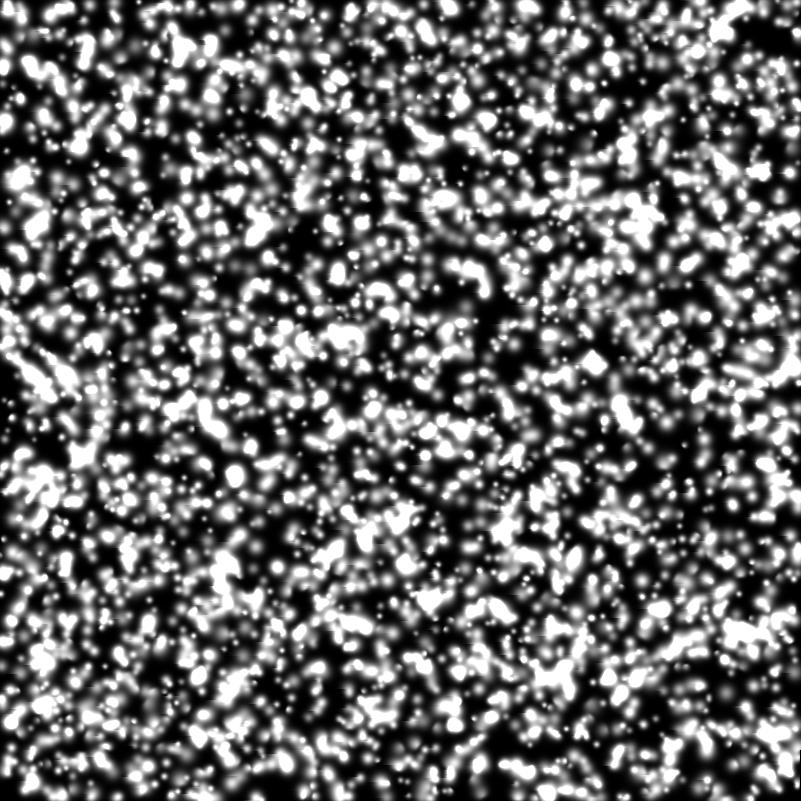
\includegraphics[scale=0.2]{image_001}
\caption{Reference image}
\label{fig: reference image synthetic}
\end{subfigure}
\hfill
\begin{subfigure}[t]{0.45\textwidth}
\centering
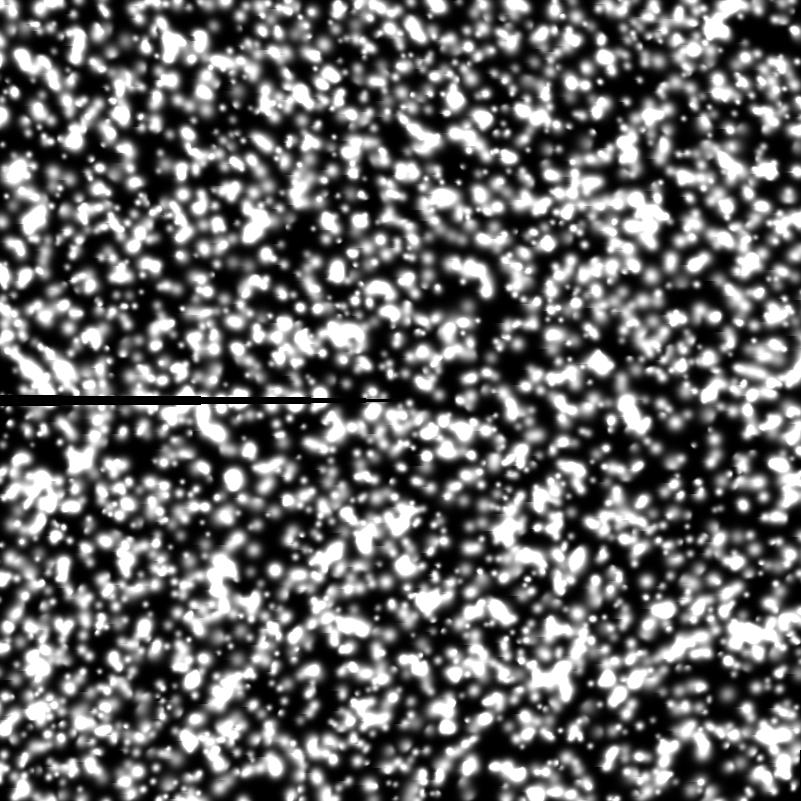
\includegraphics[scale=0.2]{image_002}
\caption{Deformed image}
\label{fig: deformed image synthetic}
\end{subfigure}
\caption{Example of a reference and deformed synthetic image}
\label{fig: synthetic images}
\end{figure}


\subsubsection{Stochastic sampling}
Sampling the speckle function at pixel centre locations is not fully representative of how digital images are actually captured. The light intensity for each pixel in a captured image is determined by the voltage generated by the pixel's corresponding CCD array element. However an element of the CCD array outputs a voltage that corresponds to all the light that falls upon its photosensitive surface and not just the light that falls at its centre as shown in Figure \ref{fig: fill factor}.

\begin{figure}[H]
\centering
\begin{subfigure}[t]{0.45\textwidth}
\centering
\begin{tikzpicture}[scale=0.6]  
    \draw [fill=gray,gray] (-1,0) rectangle (5,-1);
    \draw [fill=gray,gray] (0,0.5) rectangle (1,0);
    \draw [fill=gray,gray] (3,0) rectangle (4,0.5);
    \draw [-] (-1,0) -- (0,0) -- (0,0.5) -- (1,0.5) -- (1,0) -- (3,0) -- (3,0.5) -- (4,0.5) -- (4,0) -- (5,0);
    \filldraw [red] (1.4,0.7) circle (2pt);
    \draw [dashed,red] (1.4,0.7) -- (1.4,1.5);
    \filldraw [red] (1.8,0.6) circle (2pt);
    \draw [dashed,red] (1.8,0.6) -- (1.8,1.4);
    \filldraw [red] (2.2,0.7) circle (2pt);
    \draw [dashed,red] (2.2,0.7) -- (2.2,1.5);
    \filldraw [red] (2.6,0.6) circle (2pt);
    \draw [dashed,red] (2.6,0.6) -- (2.6,1.4);
    \filldraw [orange] (0.7,0.8) circle (2pt);
    \draw [dashed,orange] (0.7,0.8) -- (0.7,1.6);
    \draw [-] (0.5,-0.5) -- (0.5,-1.9);
    \draw [-] (3.5,-0.5) -- (3.5,-1.9);
    \draw [<->] (0.5,-1.8) -- node[above] {\scriptsize pixel size} (3.5,-1.8);
    \draw [-] (1,0.7) -- (1,2.1);
    \draw [-] (3,0.7) -- (3,2.1);
    \draw [<->] (1,2) -- node[above] {\scriptsize photosensitive area} (3,2);

    \draw [-] (4.4,2.5) rectangle (7.3,0.5);
    \node [right] at (4.4,2.1) {\scriptsize photons:};
    \filldraw [red] (4.7,1.5) circle (2pt);
    \draw [dashed,red] (4.7,1.5) -- (4.7,1.8);
    \filldraw [orange] (4.7,0.9) circle (2pt);
    \draw [dashed,orange] (4.7,0.9) -- (4.7,1.2);
    \node [right] at (4.7,1.5) {\scriptsize captured};
    \node [right] at (4.7,0.9) {\scriptsize lost};

\end{tikzpicture}
\caption{Fill factor}
\label{fig: fill factor}
\end{subfigure}
\begin{subfigure}[t]{0.45\textwidth}
\centering
\begin{tikzpicture}[scale=0.9]
   
    \draw [-] (9,-1) rectangle (12,2);
    \draw [-,blue] (9.25,-0.75) -- (11.75,-0.75);
    \draw [-,blue] (9.25,1.75) -- (11.75,1.75);
    \draw [-,blue] (9.25,-0.75) -- (9.25,1.75);
    \draw [-,blue] (11.75,-0.75) -- (11.75,1.75);

    \draw [dashed] (9.25,-0.25) -- (11.75,-0.25);
    \draw [dashed] (9.25,0.5) -- (11.75,0.5);
    \draw [dashed] (9.25,1.25) -- (11.75,1.25);

    \draw [dashed] (9.75,-0.75) -- (9.75,1.75);
    \draw [dashed] (10.5,-0.75) -- (10.5,1.75);
    \draw [dashed] (11.25,-0.75) -- (11.25,1.75);

    \filldraw [black] (9.6,-0.35) circle (1pt);
    \filldraw [black] (9.75,0.75) circle (1pt);
    \filldraw [black] (9.8,1.45) circle (1pt);

    \filldraw [black] (10.65,-0.4) circle (1pt);
    \filldraw [black] (10.3,0.6) circle (1pt);
    \filldraw [black] (10.5,1.4) circle (1pt);
    \filldraw [black] (11.4,-0.1) circle (1pt);
    \filldraw [black] (11.1,0.6) circle (1pt);
    \filldraw [black] (11.25,1.1) circle (1pt);

    \draw [-] (12.5,1.5) rectangle (13,2);
    \node [right] at (13,1.75) {\scriptsize pixel};
    \draw [-,blue] (12.5,0.75) rectangle (13,1.25);
    \node [right] at (13,1) {\scriptsize photosensitive area};
    \draw [dashed] (12.5,0.25) -- (13,0.25);
    \node [right] at (13,0.25) {\scriptsize super sampling grid};
    \filldraw [black] (12.75,-0.5) circle (1pt);
    \node [right] at (13,-0.5) {\scriptsize stochastic sampling};

    \draw [-] (9,-1.1) -- (9,-1.9);
    \draw [-] (12,-1.1) -- (12,-1.9);
    \draw [<->] (9,-1.8) -- node[above] {\scriptsize $w_{pixel}$} (12,-1.8);

    \filldraw [magenta] (10.5,0.5) circle (1pt);
    \filldraw [magenta] (12.75,-1.25) circle (1pt);
    \node [right] at (13,-1.25) {\scriptsize $(x_c,y_c)$};

    \node [left] at (9,-0.25) {\scriptsize $y_1^s$};
    \node [left] at (9,0.5) {\scriptsize $y_2^s$};
    \node [left] at (9,1.25) {\scriptsize $y_3^s$};
    \node [above] at (9.75,2) {\scriptsize $x_1^s$};
    \node [above] at (10.5,2) {\scriptsize $x_2^s$};
    \node [above] at (11.25,2) {\scriptsize $x_3^s$};

\end{tikzpicture}
\caption{Stochastic sampling}
\label{fig: stochastic}
\end{subfigure}
\caption{Illustration of the effect of the fill factor and the stochastic sampling technique}
\label{fig: fill factor stochastic}
\end{figure}

Furthermore, as seen in the figure, the photosensitive surface of a CCD array element is not the same size as the pixel it represents. This is because of the space required for the electrical components, such as electrodes and transistors, which connect the elements of the CCD array to a circuit which measures their voltages. The ratio of the photosensitive area to the total area of an element of the CCD array is referred to as the fill-factor, $\omega$.

Therefore to accurately simulate the process of the CCD array a method called stochastic sampling \todo{ref here too?} is used which is a form of super sampling. Super sampling, in this context, refers to sampling the speckle function multiple times, at different positions that fall within the photosensitive area of the same pixel (CCD array element), and averaging these function values to obtain the light intensity value for that pixel. 

The simplest method of doing this is to create a grid of points that fall within the photosensitive area of a pixel and evaluate the speckle function at these points as shown in Figure \ref{fig: stochastic}. Thus if a pixel of width and height $w_{pixel}$ has its centre located at point $(x_c,y_c)$ then the location of the super sampling grid points in the x and y directions are given as $x_j^s$ and $y_i^s$.
\begin{align}
  x_j^s &= x_c-\frac{w_{pixel}}{2} \sqrt{\omega} \left( 1+\frac{2j-1}{n} \right) \quad \text{where} \quad j=1,...,n \\
  y_i^s &= y_c-\frac{w_{pixel}}{2} \sqrt{\omega} \left( 1+\frac{2i-1}{n} \right) \quad \text{where} \quad i=1,...,n.
\end{align}
Here $n^2$ is the number of sampling points contained within the photosensitive area of a pixel. Super sampling in this manner however can lead to aliasing in the image which is not representative of the CCD array process. To avoid this the grid can be jittered whereby each grid point is translated by a random amount, less than the grid spacing, in a random direction. The speckle function is then sampled at these jittered positions shown in Figure \ref{fig: stochastic}. This is referred to as stochastic sampling. By doing this the aliasing effect is reduced at the expense of slightly increasing the noise contained in the image \cite{beets2000super}.

% .

% .

% .


% The generated image must contain a speckle pattern since it is this highly random distribution of positive and negative space that DIC relies upon to identify optical flow between images \todo{check this is correct}. First a continuous, two-dimensional function, $f_{sp}(x,y)$, is created which defines a speckle pattern that spans the range of the desired image. Thus this function gives the light intensity at any location in the image due to the speckle pattern it defines. Therefore by sampling this function at locations corresponding to the centre of pixels the image matrix can be generated. The speckle function is designed to be continuous so that no interpolation is required to sample it since this interpolation would introduce undesired bias in the generated images.

% Sampling the speckle function at pixel centre locations is however \todo{however used twice too close to one another} not fully representative of how digital images are actually captured. The light intensity for each pixel in a captured image is determined by the voltage generated by the pixel's corresponding CCD array element. However an element of the CCD array outputs a voltage that corresponds to all the light that falls upon its active surface and not just the light that falls at its centre.

% To accurately simulate this a process called stochastic sampling \todo{ref here too?} is used which is a form of super sampling. Super sampling, in this context, refers to sampling the speckle function many times, at different positions that fall within the area of the same pixel (CCD array), and averaging these function values to obtain the light intensity value for that pixel. The easiest method of doing this is to create a grid of points that fall within a pixel and evaluate the speckle function at these points. Then use a weighted average to determine the light intensity for the pixel. However this can lead to aliasing in the image where the digitized image does not accurately represent the continuous image.

% To avoid this the grid can be jittered whereby each grid point is translated by a random amount, less than the grid spacing, in a random direction. The speckle function is then sampled at these jittered positions. This is referred to as stochastic sampling. By doing this the aliasing effect is reduced at the expense of slightly increasing the noise contained in the image \cite{beets2000super}.

% Another effect that needs to be considered is the fill factor of the CCD array. To understand this first consider how light falls upon an element of the CCD array. Each element of the array has a portion of its surface, generally the perimeter, which is not sensitive to light. Thus light that falls upon this portion is not picked up by the CCD array and does not influence the image recorded. The ratio of photo-sensitive surface area to the total surface area of an element of the CCD array is termed the fill-factor. 

% This effect is simulated by not sampling the speckle function over areas that would correspond to light insensitive portions of the CCD array. More specifically if a pixel of width $w_{pixel}$ is located at point $(x_c,y_c)$ then the position of the grid points in the x direction would range from $x_c-\frac{w_{pixel}}{2}$ to $x_c+\frac{w_{pixel}}{2}$ if the fill-factor was not taken into account. But if the fill-factor is to be accounted for then the position of the grid points in the x direction would range from $x_c-\frac{w_{pixel}}{2}\times \left( 1-\frac{fillfactor}{2} \right)$ to $x_c+\frac{w_{pixel}}{2}\times \left( 1-\frac{fillfactor}{2} \right)$. Note that this is done prior to jittering the grid points.

% Once the image matrix has been generated the light intensities need to be quantised according to 12 bit quantization to simulate the camera's quantization process.

\subsubsection{Speckle function}
The function used to create a speckle pattern is based on that proposed by B. Pan et al. \cite{bing2006performance}. However, because this proposed speckle function creates speckles of constant radius, the resulting speckle pattern contains only circular speckles which is not representative of real speckle patterns created by spaying paint. 

In order to account for this the radius is modified to be a function of the angle between the radius line and the x-axis, referred to as the radius angle ($\theta_R$ in Figure \ref{fig: specklerad}). In other words the radius is a function of the arctan of the vector suspended between the speckle centre, $(x_k,y_k)$, and the investigated point in the image, $(x,y)$. \todo{end with comma'ed variable correct?}

\begin{figure}[H]
    \centering
    \begin{subfigure}[b]{0.32\textwidth}
    \centering
    \resizebox{\linewidth}{!}{
        % This file was created by matlab2tikz.
%
%The latest updates can be retrieved from
%  http://www.mathworks.com/matlabcentral/fileexchange/22022-matlab2tikz-matlab2tikz
%where you can also make suggestions and rate matlab2tikz.
%
\begin{tikzpicture}

\begin{axis}[%
width=2.153in,
height=2.153in,
at={(0.361in,0.361in)},
scale only axis,
xmin=-15,
xmax=15,
xtick={-10,   0,  10},
ymin=-15,
ymax=15,
ytick={-10,   0,  10},
axis background/.style={fill=white},
xmajorgrids,
ymajorgrids
]
\addplot [color=blue, dashed, line width=2.0pt, forget plot]
  table[row sep=crcr]{%
10	0\\
9.97986676471884	0.634239196565645\\
9.91954812830795	1.26592453573749\\
9.81928697262707	1.8925124436041\\
9.67948701396356	2.51147987181079\\
9.50071117740946	3.12033445698487\\
9.28367933016073	3.71662455660328\\
9.02926538286621	4.29794912089172\\
8.73849377069785	4.86196736100469\\
8.41253532831181	5.40640817455598\\
8.05270257531059	5.9290792905464\\
7.66044443118978	6.42787609686539\\
7.2373403810507	6.90079011482112\\
6.78509411557132	7.34591708657533\\
6.30552667084523	7.76146464291757\\
5.80056909571198	8.14575952050336\\
5.27225467610502	8.49725429949514\\
4.72271074772683	8.81453363447582\\
4.15415013001886	9.09631995354518\\
3.56886221591872	9.34147860265107\\
2.96920375328275	9.54902241444074\\
2.35758935509427	9.71811568323542\\
1.73648177666931	9.84807753012208\\
1.10838199901011	9.93838464461254\\
0.475819158237424	9.98867339183008\\
-0.15865963834808	9.99874127673875\\
-0.792499568567885	9.96854775951942\\
-1.42314838273285	9.89821441880933\\
-2.04806668065191	9.78802446214779\\
-2.66473813690035	9.63842158559942\\
-3.27067963317421	9.45000818714669\\
-3.86345125693128	9.22354294104581\\
-4.44066612605774	8.95993774291336\\
-5	8.66025403784439\\
-5.5392006386611	8.32569854634771\\
-6.05609687137667	7.95761840530832\\
-6.54860733945285	7.55749574354258\\
-7.01474887706321	7.12694171378863\\
-7.45264449675755	6.66769000516292\\
-7.86053094742787	6.18158986220605\\
-8.23676581429833	5.67059863862771\\
-8.57983413234977	5.13677391573407\\
-8.88835448654923	4.58226521727411\\
-9.16108457432069	4.00930535406614\\
-9.39692620785908	3.42020143325669\\
-9.59492973614497	2.8173255684143\\
-9.75429786885407	2.20310532786541\\
-9.87438888676394	1.5800139597335\\
-9.95471922573085	0.950560433041829\\
-9.99496542383185	0.317279334980681\\
-9.99496542383185	-0.317279334980679\\
-9.95471922573085	-0.950560433041826\\
-9.87438888676394	-1.5800139597335\\
-9.75429786885407	-2.20310532786541\\
-9.59492973614497	-2.81732556841429\\
-9.39692620785909	-3.42020143325669\\
-9.1610845743207	-4.00930535406613\\
-8.88835448654924	-4.5822652172741\\
-8.57983413234977	-5.13677391573406\\
-8.23676581429833	-5.67059863862771\\
-7.86053094742788	-6.18158986220605\\
-7.45264449675755	-6.66769000516291\\
-7.01474887706322	-7.12694171378863\\
-6.54860733945285	-7.55749574354258\\
-6.05609687137667	-7.95761840530832\\
-5.5392006386611	-8.32569854634771\\
-5	-8.66025403784439\\
-4.44066612605774	-8.95993774291336\\
-3.86345125693129	-9.22354294104581\\
-3.27067963317422	-9.45000818714668\\
-2.66473813690035	-9.63842158559942\\
-2.04806668065191	-9.78802446214779\\
-1.42314838273285	-9.89821441880933\\
-0.792499568567888	-9.96854775951942\\
-0.158659638348076	-9.99874127673875\\
0.475819158237424	-9.98867339183008\\
1.10838199901011	-9.93838464461254\\
1.7364817766693	-9.84807753012208\\
2.35758935509427	-9.71811568323542\\
2.96920375328275	-9.54902241444074\\
3.56886221591872	-9.34147860265107\\
4.15415013001886	-9.09631995354519\\
4.72271074772682	-8.81453363447582\\
5.27225467610502	-8.49725429949514\\
5.80056909571198	-8.14575952050336\\
6.30552667084522	-7.76146464291757\\
6.78509411557132	-7.34591708657534\\
7.23734038105069	-6.90079011482113\\
7.66044443118977	-6.4278760968654\\
8.05270257531059	-5.9290792905464\\
8.41253532831181	-5.40640817455597\\
8.73849377069785	-4.86196736100469\\
9.02926538286621	-4.29794912089172\\
9.28367933016072	-3.71662455660328\\
9.50071117740946	-3.12033445698487\\
9.67948701396356	-2.51147987181079\\
9.81928697262707	-1.89251244360411\\
9.91954812830795	-1.2659245357375\\
9.97986676471884	-0.634239196565654\\
10	-2.44929359829471e-15\\
};
\addplot [color=red, line width=2.0pt, forget plot]
  table[row sep=crcr]{%
10	0\\
10.2963627183444	0.654353106307745\\
10.5474474971886	1.34605653436873\\
10.7484866208707	2.07160099675422\\
10.8950357713948	2.82687119710409\\
10.9830504094947	3.60718160941848\\
11.0089576437591	4.40732180273315\\
10.9697224040741	5.22161070295733\\
10.8629068196563	6.04395903787279\\
10.6867218038138	6.86793907716508\\
10.4400699656499	7.68686065905057\\
10.1225791013725	8.49385239052451\\
9.73462566256205	9.28194682118014\\
9.27734775340198	10.0441683223547\\
8.75264737101623	10.7736223551588\\
8.16318177010632	11.4635847835343\\
7.51234400237501	12.1075898823284\\
6.8042328500613	12.6995157055805\\
6.0436125385976	13.2336655165834\\
5.23586277328933	13.7048440382304\\
4.3869197964548	14.1084273588117\\
3.50320930222756	14.4404254235668\\
2.59157217396491	14.6975361544343\\
1.65918412188236	14.8771903677859\\
0.713470394342912	14.9775868004783\\
-0.237983186360274	14.997716706059\\
-1.18752155511639	14.9373776430296\\
-2.1275127561822	14.7971762431441\\
-3.05043995456266	14.5785199171682\\
-3.94899175006848	14.2835976256519\\
-4.81614946421838	13.9153500103633\\
-5.64527011774126	13.4774293454262\\
-6.43016388415987	12.9741499233021\\
-7.16516489172098	12.4104296370695\\
-7.84519435038877	11.7917236546671\\
-8.4658151010673	11.1239512007469\\
-9.02327681874064	10.4134165656261\\
-9.51455124766258	9.66672554689302\\
-9.93735700275351	8.89069859615912\\
-10.2901736344756	8.09228199019164\\
-10.5722448220547	7.27845837150213\\
-10.7835707293205	6.45615800799592\\
-10.9248897259457	5.63217210446696\\
-10.9976498417877	4.81306946083878\\
-11.0039704807462	4.00511771373558\\
-10.946595070523	3.21421032017409\\
-10.8288354635127	2.44580034616529\\
-10.6545090295643	1.70484201036316\\
-10.4278694915464	0.9957408054229\\
-10.1535326477674	0.322312879493004\\
-9.83639819989634	-0.312245790468355\\
-9.48156895991525	-0.905380060660755\\
-9.09426874396354	-1.45518590910384\\
-8.67976027419546	-1.96041030956552\\
-8.24326440176691	-2.4204408166545\\
-7.78988193497196	-2.8352851527778\\
-7.32451930685366	-3.20554124729349\\
-6.85181924715275	-3.53235833008125\\
-6.37609753537909	-3.81738982347221\\
-5.90128680654196	-4.06273890575329\\
-5.43088826038012	-4.27089773422047\\
-4.96793199076158	-4.44468141416672\\
-4.51494650646385	-4.58715788068423\\
-4.07393786016506	-4.70157492145908\\
-3.64637864168603	-4.7912856098697\\
-3.23320692693344	-4.85967343802836\\
-2.83483510827902	-4.91007843861928\\
-2.45116836795561	-4.9457255625246\\
-2.08163239612131	-4.96965653666546\\
-1.72520980213006	-4.98466636393009\\
-1.38048452373223	-4.99324554554689\\
-1.04569340674115	-4.99752900712738\\
-0.718784009283498	-4.99925259447457\\
-0.397477582019379	-4.99971787600924\\
-0.0793360903358842	-4.99976584741849\\
0.238167922131936	-4.99975998318182\\
0.557579876137864	-4.99957892143914\\
0.881391379373703	-4.99861890580987\\
1.21196940796098	-4.99580594290402\\
1.5514877101107	-4.98961747006979\\
1.90186165854811	-4.9781131670717\\
2.26468772144013	-4.95897439050694\\
2.64118864539235	-4.92955156337115\\
3.03216534983504	-4.88691871666192\\
3.43795642131765	-4.82793425747245\\
3.85840597067421	-4.74930693067638\\
4.29284047774066	-4.64766585079595\\
4.74005509953934	-4.5196334084621\\
5.19830976100705	-4.36189980320628\\
5.6653351849713	-4.17129792204224\\
6.13834885280984	-3.94487727194687\\
6.61408072173936	-3.67997568413658\\
7.08880836165835	-3.37428753882611\\
7.55840101656232	-3.0259273104734\\
8.01837194532425	-2.63348730455126\\
8.46393825653232	-2.1960885465175\\
8.89008732438344	-1.71342389045398\\
9.29164875942729	-1.18579253710626\\
9.6633708110933	-0.614125286823553\\
10	-2.44929359829471e-15\\
};
\draw [line width=0.25mm,->] (0,0) -- (15,0);
\draw [line width=0.25mm,->] (0,0) -- (9.571184878015547,9.571184878015547);
\draw[line width=0.25mm,black] (3,0) arc (0: 45:3);
\draw (0,0) circle[radius=1.5pt];
\fill (0,0) circle[radius=1.5pt];
\draw [line width=0.25mm,dotted] (9.571184878015547,9.571184878015547) -- (11,11);
\draw (11,11) circle[radius=1.5pt];
\fill (11,11) circle[radius=1.5pt];
\node [below] at (0,0) {\small $(x_k,y_k)$};
\node [above] at (11,11) {\small $(x,y)$};
% \node [above,left] at (4.3962,4.1918) {\small $R$};
\node [above,right] at (3.1144,1.6) {\small $\theta_R$};
\end{axis}
\end{tikzpicture}%
        }
        \caption{\footnotesize $a=0$, $b=1$, $R_{k}=10$}
        \label{fig: specklerad 0 1}
    \end{subfigure}
    \hfill
     %add desired spacing between images, e. g. ~, \quad, \qquad, \hfill etc. 
      %(or a blank line to force the subfigure onto a new line)
    \begin{subfigure}[b]{0.32\textwidth}
    \centering
    \resizebox{\linewidth}{!}{
        % This file was created by matlab2tikz.
%
%The latest updates can be retrieved from
%  http://www.mathworks.com/matlabcentral/fileexchange/22022-matlab2tikz-matlab2tikz
%where you can also make suggestions and rate matlab2tikz.
%
\begin{tikzpicture}

\begin{axis}[%
width=2.153in,
height=2.153in,
at={(0.361in,0.361in)},
scale only axis,
xmin=-15,
xmax=15,
xtick={-10,   0,  10},
ymin=-15,
ymax=15,
ytick={-10,   0,  10},
axis background/.style={fill=white},
xmajorgrids,
ymajorgrids
]
\addplot [color=blue, dashed, line width=2.0pt, forget plot]
  table[row sep=crcr]{%
10	0\\
9.97986676471884	0.634239196565645\\
9.91954812830795	1.26592453573749\\
9.81928697262707	1.8925124436041\\
9.67948701396356	2.51147987181079\\
9.50071117740946	3.12033445698487\\
9.28367933016073	3.71662455660328\\
9.02926538286621	4.29794912089172\\
8.73849377069785	4.86196736100469\\
8.41253532831181	5.40640817455598\\
8.05270257531059	5.9290792905464\\
7.66044443118978	6.42787609686539\\
7.2373403810507	6.90079011482112\\
6.78509411557132	7.34591708657533\\
6.30552667084523	7.76146464291757\\
5.80056909571198	8.14575952050336\\
5.27225467610502	8.49725429949514\\
4.72271074772683	8.81453363447582\\
4.15415013001886	9.09631995354518\\
3.56886221591872	9.34147860265107\\
2.96920375328275	9.54902241444074\\
2.35758935509427	9.71811568323542\\
1.73648177666931	9.84807753012208\\
1.10838199901011	9.93838464461254\\
0.475819158237424	9.98867339183008\\
-0.15865963834808	9.99874127673875\\
-0.792499568567885	9.96854775951942\\
-1.42314838273285	9.89821441880933\\
-2.04806668065191	9.78802446214779\\
-2.66473813690035	9.63842158559942\\
-3.27067963317421	9.45000818714669\\
-3.86345125693128	9.22354294104581\\
-4.44066612605774	8.95993774291336\\
-5	8.66025403784439\\
-5.5392006386611	8.32569854634771\\
-6.05609687137667	7.95761840530832\\
-6.54860733945285	7.55749574354258\\
-7.01474887706321	7.12694171378863\\
-7.45264449675755	6.66769000516292\\
-7.86053094742787	6.18158986220605\\
-8.23676581429833	5.67059863862771\\
-8.57983413234977	5.13677391573407\\
-8.88835448654923	4.58226521727411\\
-9.16108457432069	4.00930535406614\\
-9.39692620785908	3.42020143325669\\
-9.59492973614497	2.8173255684143\\
-9.75429786885407	2.20310532786541\\
-9.87438888676394	1.5800139597335\\
-9.95471922573085	0.950560433041829\\
-9.99496542383185	0.317279334980681\\
-9.99496542383185	-0.317279334980679\\
-9.95471922573085	-0.950560433041826\\
-9.87438888676394	-1.5800139597335\\
-9.75429786885407	-2.20310532786541\\
-9.59492973614497	-2.81732556841429\\
-9.39692620785909	-3.42020143325669\\
-9.1610845743207	-4.00930535406613\\
-8.88835448654924	-4.5822652172741\\
-8.57983413234977	-5.13677391573406\\
-8.23676581429833	-5.67059863862771\\
-7.86053094742788	-6.18158986220605\\
-7.45264449675755	-6.66769000516291\\
-7.01474887706322	-7.12694171378863\\
-6.54860733945285	-7.55749574354258\\
-6.05609687137667	-7.95761840530832\\
-5.5392006386611	-8.32569854634771\\
-5	-8.66025403784439\\
-4.44066612605774	-8.95993774291336\\
-3.86345125693129	-9.22354294104581\\
-3.27067963317422	-9.45000818714668\\
-2.66473813690035	-9.63842158559942\\
-2.04806668065191	-9.78802446214779\\
-1.42314838273285	-9.89821441880933\\
-0.792499568567888	-9.96854775951942\\
-0.158659638348076	-9.99874127673875\\
0.475819158237424	-9.98867339183008\\
1.10838199901011	-9.93838464461254\\
1.7364817766693	-9.84807753012208\\
2.35758935509427	-9.71811568323542\\
2.96920375328275	-9.54902241444074\\
3.56886221591872	-9.34147860265107\\
4.15415013001886	-9.09631995354519\\
4.72271074772682	-8.81453363447582\\
5.27225467610502	-8.49725429949514\\
5.80056909571198	-8.14575952050336\\
6.30552667084522	-7.76146464291757\\
6.78509411557132	-7.34591708657534\\
7.23734038105069	-6.90079011482113\\
7.66044443118977	-6.4278760968654\\
8.05270257531059	-5.9290792905464\\
8.41253532831181	-5.40640817455597\\
8.73849377069785	-4.86196736100469\\
9.02926538286621	-4.29794912089172\\
9.28367933016072	-3.71662455660328\\
9.50071117740946	-3.12033445698487\\
9.67948701396356	-2.51147987181079\\
9.81928697262707	-1.89251244360411\\
9.91954812830795	-1.2659245357375\\
9.97986676471884	-0.634239196565654\\
10	-2.44929359829471e-15\\
};
\addplot [color=red, line width=2.0pt, forget plot]
  table[row sep=crcr]{%
15.0002341323001	0\\
14.9599869872769	0.950735150191186\\
14.8396502619769	1.89382390461815\\
14.6404325517771	2.82171209184773\\
14.3643298209704	3.72702862924204\\
14.014098157276	4.60267368907007\\
13.593216216331	5.44190287020168\\
13.1058379331007	6.23840614209957\\
12.5567362261299	6.98638040996318\\
11.9512385580029	7.68059465005795\\
11.2951553391066	8.31644668088569\\
10.5947022698308	8.89001076704812\\
9.85641780699183	9.39807539633247\\
9.08707701209208	9.83817072440599\\
8.29360309090418	10.2085853430886\\
7.48297796498122	10.5083721948977\\
6.66215322557195	10.7373436257651\\
5.8379628089223	10.8960557368103\\
5.01703869928077	10.9857823621239\\
4.20573091263949	11.0084791600217\\
3.41003294121195	10.9667384576128\\
2.63551374706302	10.8637356303687\\
1.88725728465724	10.7031679274177\\
1.16981040813685	10.4891867674848\\
0.487139881889304	10.2263246279356\\
-0.157400935368198	9.91941772872656\\
-0.761095319777928	9.57352577297092\\
-1.32187607476746	9.19385004535998\\
-1.83832800337217	8.78565118823703\\
-2.30968004465273	8.35416797243129\\
-2.73578732409067	7.90453835610252\\
-3.11710352901149	7.44172408023584\\
-3.45464417414636	6.97043998481123\\
-3.74994146692496	6.49508914612341\\
-4.00499161468032	6.01970483462005\\
-4.22219553451515	5.54790017561769\\
-4.40429402923621	5.08282626425479\\
-4.55429857786746	4.62713934318926\\
-4.6754189554536	4.18297749916695\\
-4.77098894311331	3.7519471751583\\
-4.8443914148726	3.33511963087134\\
-4.89898409231148	2.93303731876338\\
-4.93802724144194	2.54572997787762\\
-4.9646145487932	2.1727400865991\\
-4.98160835603783	1.81315716036956\\
-4.99158035560463	1.46566023403623\\
-4.99675875485381	1.1285677332068\\
-4.99898280509346	0.7998938169331\\
-4.99966546581177	0.477410167226229\\
-4.99976483604403	0.158712111045171\\
-4.99976483604403	-0.15871211104517\\
-4.99966546581177	-0.477410167226227\\
-4.99898280509346	-0.799893816933101\\
-4.99675875485381	-1.1285677332068\\
-4.99158035560463	-1.46566023403623\\
-4.98160835603783	-1.81315716036956\\
-4.96461454879319	-2.17274008659909\\
-4.93802724144194	-2.54572997787761\\
-4.89898409231148	-2.93303731876338\\
-4.8443914148726	-3.33511963087134\\
-4.77098894311331	-3.7519471751583\\
-4.6754189554536	-4.18297749916695\\
-4.55429857786747	-4.62713934318925\\
-4.40429402923621	-5.08282626425479\\
-4.22219553451515	-5.54790017561769\\
-4.00499161468032	-6.01970483462005\\
-3.74994146692497	-6.4950891461234\\
-3.45464417414635	-6.97043998481123\\
-3.11710352901149	-7.44172408023583\\
-2.73578732409067	-7.90453835610252\\
-2.30968004465274	-8.35416797243129\\
-1.83832800337217	-8.78565118823703\\
-1.32187607476747	-9.19385004535997\\
-0.76109531977793	-9.57352577297091\\
-0.157400935368194	-9.91941772872656\\
0.487139881889304	-10.2263246279356\\
1.16981040813685	-10.4891867674848\\
1.88725728465723	-10.7031679274177\\
2.63551374706301	-10.8637356303687\\
3.41003294121195	-10.9667384576128\\
4.20573091263949	-11.0084791600217\\
5.01703869928076	-10.9857823621239\\
5.83796280892229	-10.8960557368103\\
6.66215322557195	-10.7373436257651\\
7.48297796498122	-10.5083721948977\\
8.29360309090417	-10.2085853430886\\
9.08707701209207	-9.83817072440599\\
9.85641780699181	-9.39807539633248\\
10.5947022698308	-8.89001076704813\\
11.2951553391066	-8.31644668088569\\
11.9512385580029	-7.68059465005795\\
12.5567362261299	-6.98638040996318\\
13.1058379331007	-6.23840614209958\\
13.593216216331	-5.44190287020168\\
14.014098157276	-4.60267368907007\\
14.3643298209704	-3.72702862924204\\
14.6404325517771	-2.82171209184774\\
14.8396502619769	-1.89382390461816\\
14.9599869872769	-0.9507351501912\\
15.0002341323001	-3.67399774331645e-15\\
};
\draw [line width=0.25mm,->] (0,0) -- (15,0);
\draw [line width=0.25mm,->] (0,0) -- (9.571184878015547,9.571184878015547);
\draw[line width=0.25mm,black] (3,0) arc (0: 45:3);
\draw (0,0) circle[radius=1.5pt];
\fill (0,0) circle[radius=1.5pt];
\draw [line width=0.25mm,dotted] (9.571184878015547,9.571184878015547) -- (11,11);
\draw (11,11) circle[radius=1.5pt];
\fill (11,11) circle[radius=1.5pt];
\node [below] at (0,0) {\small $(x_k,y_k)$};
\node [above] at (11,11) {\small $(x,y)$};
% \node [above,left] at (4.3962,4.1918) {\small $R$};
\node [above,right] at (3.1144,1.6) {\small $\theta_R$};
\end{axis}
\end{tikzpicture}%
        }
        \caption{\footnotesize $a=\frac{\pi}{2}$, $b=1$, $R_{k}=10$}
        \label{fig: specklerad 157 1}
    \end{subfigure}
    % \vskip\baselineskip
    \hfill
    \begin{subfigure}[b]{0.32\textwidth}
    \centering
    \resizebox{\linewidth}{!}{
        % This file was created by matlab2tikz.
%
%The latest updates can be retrieved from
%  http://www.mathworks.com/matlabcentral/fileexchange/22022-matlab2tikz-matlab2tikz
%where you can also make suggestions and rate matlab2tikz.
%
\begin{tikzpicture}

\begin{axis}[%
width=2.153in,
height=2.153in,
at={(0.361in,0.361in)},
scale only axis,
xmin=-15,
xmax=15,
xtick={-10,   0,  10},
ymin=-15,
ymax=15,
ytick={-10,   0,  10},
axis background/.style={fill=white},
xmajorgrids,
ymajorgrids
]
\addplot [color=blue, dashed, line width=2.0pt, forget plot]
  table[row sep=crcr]{%
10	0\\
9.97986676471884	0.634239196565645\\
9.91954812830795	1.26592453573749\\
9.81928697262707	1.8925124436041\\
9.67948701396356	2.51147987181079\\
9.50071117740946	3.12033445698487\\
9.28367933016073	3.71662455660328\\
9.02926538286621	4.29794912089172\\
8.73849377069785	4.86196736100469\\
8.41253532831181	5.40640817455598\\
8.05270257531059	5.9290792905464\\
7.66044443118978	6.42787609686539\\
7.2373403810507	6.90079011482112\\
6.78509411557132	7.34591708657533\\
6.30552667084523	7.76146464291757\\
5.80056909571198	8.14575952050336\\
5.27225467610502	8.49725429949514\\
4.72271074772683	8.81453363447582\\
4.15415013001886	9.09631995354518\\
3.56886221591872	9.34147860265107\\
2.96920375328275	9.54902241444074\\
2.35758935509427	9.71811568323542\\
1.73648177666931	9.84807753012208\\
1.10838199901011	9.93838464461254\\
0.475819158237424	9.98867339183008\\
-0.15865963834808	9.99874127673875\\
-0.792499568567885	9.96854775951942\\
-1.42314838273285	9.89821441880933\\
-2.04806668065191	9.78802446214779\\
-2.66473813690035	9.63842158559942\\
-3.27067963317421	9.45000818714669\\
-3.86345125693128	9.22354294104581\\
-4.44066612605774	8.95993774291336\\
-5	8.66025403784439\\
-5.5392006386611	8.32569854634771\\
-6.05609687137667	7.95761840530832\\
-6.54860733945285	7.55749574354258\\
-7.01474887706321	7.12694171378863\\
-7.45264449675755	6.66769000516292\\
-7.86053094742787	6.18158986220605\\
-8.23676581429833	5.67059863862771\\
-8.57983413234977	5.13677391573407\\
-8.88835448654923	4.58226521727411\\
-9.16108457432069	4.00930535406614\\
-9.39692620785908	3.42020143325669\\
-9.59492973614497	2.8173255684143\\
-9.75429786885407	2.20310532786541\\
-9.87438888676394	1.5800139597335\\
-9.95471922573085	0.950560433041829\\
-9.99496542383185	0.317279334980681\\
-9.99496542383185	-0.317279334980679\\
-9.95471922573085	-0.950560433041826\\
-9.87438888676394	-1.5800139597335\\
-9.75429786885407	-2.20310532786541\\
-9.59492973614497	-2.81732556841429\\
-9.39692620785909	-3.42020143325669\\
-9.1610845743207	-4.00930535406613\\
-8.88835448654924	-4.5822652172741\\
-8.57983413234977	-5.13677391573406\\
-8.23676581429833	-5.67059863862771\\
-7.86053094742788	-6.18158986220605\\
-7.45264449675755	-6.66769000516291\\
-7.01474887706322	-7.12694171378863\\
-6.54860733945285	-7.55749574354258\\
-6.05609687137667	-7.95761840530832\\
-5.5392006386611	-8.32569854634771\\
-5	-8.66025403784439\\
-4.44066612605774	-8.95993774291336\\
-3.86345125693129	-9.22354294104581\\
-3.27067963317422	-9.45000818714668\\
-2.66473813690035	-9.63842158559942\\
-2.04806668065191	-9.78802446214779\\
-1.42314838273285	-9.89821441880933\\
-0.792499568567888	-9.96854775951942\\
-0.158659638348076	-9.99874127673875\\
0.475819158237424	-9.98867339183008\\
1.10838199901011	-9.93838464461254\\
1.7364817766693	-9.84807753012208\\
2.35758935509427	-9.71811568323542\\
2.96920375328275	-9.54902241444074\\
3.56886221591872	-9.34147860265107\\
4.15415013001886	-9.09631995354519\\
4.72271074772682	-8.81453363447582\\
5.27225467610502	-8.49725429949514\\
5.80056909571198	-8.14575952050336\\
6.30552667084522	-7.76146464291757\\
6.78509411557132	-7.34591708657534\\
7.23734038105069	-6.90079011482113\\
7.66044443118977	-6.4278760968654\\
8.05270257531059	-5.9290792905464\\
8.41253532831181	-5.40640817455597\\
8.73849377069785	-4.86196736100469\\
9.02926538286621	-4.29794912089172\\
9.28367933016072	-3.71662455660328\\
9.50071117740946	-3.12033445698487\\
9.67948701396356	-2.51147987181079\\
9.81928697262707	-1.89251244360411\\
9.91954812830795	-1.2659245357375\\
9.97986676471884	-0.634239196565654\\
10	-2.44929359829471e-15\\
};
\addplot [color=red, line width=2.0pt, forget plot]
  table[row sep=crcr]{%
10	0\\
10.3031040549212	0.654781530854394\\
10.5569458215773	1.34726870267887\\
10.7530088646046	2.07247258779369\\
10.8835612873369	2.82389397984978\\
10.9419377825713	3.59367892061859\\
10.9227883732228	4.37282483062647\\
10.8222848211688	5.151430106534\\
10.6382771915936	5.91897846929726\\
10.3703948408983	6.66464808207312\\
10.0200880844544	7.37763455130438\\
9.59060892437961	8.04747641121246\\
9.08693140041786	8.66437158963049\\
8.51561429009251	9.21947366547448\\
7.88461094947689	9.70515744394157\\
7.20303297861345	10.1152444689288\\
6.4808760474854	10.4451805237288\\
5.72871756986352	10.692158889104\\
4.9573969145384	10.8551850703466\\
4.17768946024611	10.9350808017573\\
3.39998600976545	10.9344273124201\\
2.63398887270443	10.857450012652\\
1.88843531289292	10.7098488575337\\
1.17085805728203	10.4985805867517\\
0.487391214963884	10.2316007584803\\
-0.157371693864653	9.9175749271701\\
-0.760462788842132	9.56556940921636\\
-1.32056521236519	9.18473279708942\\
-1.8379782568067	8.7839796958141\\
-2.31452382848983	8.37168805444046\\
-2.75339796213336	7.95542095310052\\
-3.15897308517341	7.54168280198472\\
-3.53655850972583	7.13571864486122\\
-3.89212813671344	6.74136368235606\\
-4.23202553739688	6.36094829620186\\
-4.56265738956069	5.99526183140969\\
-4.89018665959174	5.64357625205869\\
-5.22023692271016	5.30372860559172\\
-5.55761880166994	4.97225908904181\\
-5.90608869426351	4.64459948595401\\
-6.26814878125911	4.31530490815002\\
-6.64489580162099	3.97832019827047\\
-7.03592430544753	3.62727108431772\\
-7.43928811127225	3.25576927196702\\
-7.85152157496561	2.85772014698638\\
-8.26772009911639	2.42762165729959\\
-8.68167715325824	1.96084325579424\\
-9.08607301472485	1.45387449968338\\
-9.4727085518126	0.904533994270335\\
-9.83277572362099	0.312130798888608\\
-10.1571551240427	-0.322427871072751\\
-10.4367298996491	-0.996586871813319\\
-10.662704758803	-1.70615341978362\\
-10.8269185844499	-2.44536739993658\\
-10.9221393731736	-3.207029479529\\
-10.9423308407526	-3.982682719527\\
-10.8828810373691	-4.76284143616525\\
-10.7407846676509	-5.53725935023049\\
-10.5147724630785	-6.29522763319766\\
-10.2053828473375	-7.02589236910539\\
-9.81497320059224	-7.71858023845809\\
-9.34767019184516	-8.36312092128402\\
-8.80926083141627	-8.95015482198553\\
-8.20702801931396	-9.47141523502648\\
-7.54953635319264	-9.91997497920695\\
-6.84637573992533	-10.2904487964936\\
-6.10787186328657	-10.5791443933327\\
-5.34477374238965	-10.7841568409655\\
-4.56792942868916	-10.9054030801069\\
-3.78796130421507	-10.9445954211928\\
-3.01495244531088	-10.9051551167584\\
-2.25815510449711	-10.7920692284815\\
-1.52573155310051	-10.6116960405292\\
-0.824536348293641	-10.3715261098225\\
-0.159947582831504	-10.0799076263074\\
0.464247101510964	-9.74574602517986\\
1.04590594073819	-9.37818870247338\\
1.58452824044569	-8.98630620271051\\
2.08118983748411	-8.57878135381886\\
2.53842149680004	-8.16361751646135\\
2.96003497159133	-7.74787640354481\\
3.35090334549933	-7.33745483674382\\
3.71670392559013	-6.93690837984761\\
4.06363330472464	-6.54932807526146\\
4.39810521281052	-6.17627457207789\\
4.72644239221355	-5.81777184189357\\
5.05457394105012	-5.47236050767619\\
5.38774936168354	-5.13720864001176\\
5.73027993799995	-4.80827578251834\\
6.08531706616682	-4.48052402978843\\
6.45467581572532	-4.14816826703883\\
6.83871034980208	-3.80495625271212\\
7.23624594456362	-3.44446813524944\\
7.64457028709866	-3.06042428258008\\
8.05948457224764	-2.64698999335115\\
8.47541274059021	-2.19906576377181\\
8.88556508064958	-1.71255229941451\\
9.28215043503863	-1.18458036879612\\
9.65662947451644	-0.613696862276905\\
10	-2.44929359829471e-15\\
};
\draw [line width=0.25mm,->] (0,0) -- (15,0);
\draw [line width=0.25mm,->] (0,0) -- (8.880214988824488,8.880214988824488);
\draw[line width=0.25mm,black] (3,0) arc (0: 45:3);
\draw (0,0) circle[radius=1.5pt];
\fill (0,0) circle[radius=1.5pt];
\draw [line width=0.25mm,dotted] (8.880214988824488,8.880214988824488) -- (11,11);
\draw (11,11) circle[radius=1.5pt];
\fill (11,11) circle[radius=1.5pt];
\node [below] at (0,0) {\small $(x_k,y_k)$};
\node [above] at (11,11) {\small $(x,y)$};
% \node [above,left] at (4.3962,4.1918) {\small $R$};
\node [above,right] at (3.1144,1.6) {\small $\theta_R$};
\end{axis}
\end{tikzpicture}%
        }
        \caption{\footnotesize $a=0$, $b=2$, $R_{k}=10$}
        % \label{fig: specklerad 2}
    \end{subfigure}
    
    \begin{subfigure}[b]{0.32\textwidth}
    \centering
    \resizebox{\linewidth}{!}{
        % This file was created by matlab2tikz.
%
%The latest updates can be retrieved from
%  http://www.mathworks.com/matlabcentral/fileexchange/22022-matlab2tikz-matlab2tikz
%where you can also make suggestions and rate matlab2tikz.
%
\begin{tikzpicture}

\begin{axis}[%
width=2.153in,
height=2.153in,
at={(0.361in,0.361in)},
scale only axis,
xmin=-15,
xmax=15,
xtick={-10,   0,  10},
ymin=-15,
ymax=15,
ytick={-10,   0,  10},
axis background/.style={fill=white},
xmajorgrids,
ymajorgrids
]
\addplot [color=blue, dashed, line width=2.0pt, forget plot]
  table[row sep=crcr]{%
10	0\\
9.97986676471884	0.634239196565645\\
9.91954812830795	1.26592453573749\\
9.81928697262707	1.8925124436041\\
9.67948701396356	2.51147987181079\\
9.50071117740946	3.12033445698487\\
9.28367933016073	3.71662455660328\\
9.02926538286621	4.29794912089172\\
8.73849377069785	4.86196736100469\\
8.41253532831181	5.40640817455598\\
8.05270257531059	5.9290792905464\\
7.66044443118978	6.42787609686539\\
7.2373403810507	6.90079011482112\\
6.78509411557132	7.34591708657533\\
6.30552667084523	7.76146464291757\\
5.80056909571198	8.14575952050336\\
5.27225467610502	8.49725429949514\\
4.72271074772683	8.81453363447582\\
4.15415013001886	9.09631995354518\\
3.56886221591872	9.34147860265107\\
2.96920375328275	9.54902241444074\\
2.35758935509427	9.71811568323542\\
1.73648177666931	9.84807753012208\\
1.10838199901011	9.93838464461254\\
0.475819158237424	9.98867339183008\\
-0.15865963834808	9.99874127673875\\
-0.792499568567885	9.96854775951942\\
-1.42314838273285	9.89821441880933\\
-2.04806668065191	9.78802446214779\\
-2.66473813690035	9.63842158559942\\
-3.27067963317421	9.45000818714669\\
-3.86345125693128	9.22354294104581\\
-4.44066612605774	8.95993774291336\\
-5	8.66025403784439\\
-5.5392006386611	8.32569854634771\\
-6.05609687137667	7.95761840530832\\
-6.54860733945285	7.55749574354258\\
-7.01474887706321	7.12694171378863\\
-7.45264449675755	6.66769000516292\\
-7.86053094742787	6.18158986220605\\
-8.23676581429833	5.67059863862771\\
-8.57983413234977	5.13677391573407\\
-8.88835448654923	4.58226521727411\\
-9.16108457432069	4.00930535406614\\
-9.39692620785908	3.42020143325669\\
-9.59492973614497	2.8173255684143\\
-9.75429786885407	2.20310532786541\\
-9.87438888676394	1.5800139597335\\
-9.95471922573085	0.950560433041829\\
-9.99496542383185	0.317279334980681\\
-9.99496542383185	-0.317279334980679\\
-9.95471922573085	-0.950560433041826\\
-9.87438888676394	-1.5800139597335\\
-9.75429786885407	-2.20310532786541\\
-9.59492973614497	-2.81732556841429\\
-9.39692620785909	-3.42020143325669\\
-9.1610845743207	-4.00930535406613\\
-8.88835448654924	-4.5822652172741\\
-8.57983413234977	-5.13677391573406\\
-8.23676581429833	-5.67059863862771\\
-7.86053094742788	-6.18158986220605\\
-7.45264449675755	-6.66769000516291\\
-7.01474887706322	-7.12694171378863\\
-6.54860733945285	-7.55749574354258\\
-6.05609687137667	-7.95761840530832\\
-5.5392006386611	-8.32569854634771\\
-5	-8.66025403784439\\
-4.44066612605774	-8.95993774291336\\
-3.86345125693129	-9.22354294104581\\
-3.27067963317422	-9.45000818714668\\
-2.66473813690035	-9.63842158559942\\
-2.04806668065191	-9.78802446214779\\
-1.42314838273285	-9.89821441880933\\
-0.792499568567888	-9.96854775951942\\
-0.158659638348076	-9.99874127673875\\
0.475819158237424	-9.98867339183008\\
1.10838199901011	-9.93838464461254\\
1.7364817766693	-9.84807753012208\\
2.35758935509427	-9.71811568323542\\
2.96920375328275	-9.54902241444074\\
3.56886221591872	-9.34147860265107\\
4.15415013001886	-9.09631995354519\\
4.72271074772682	-8.81453363447582\\
5.27225467610502	-8.49725429949514\\
5.80056909571198	-8.14575952050336\\
6.30552667084522	-7.76146464291757\\
6.78509411557132	-7.34591708657534\\
7.23734038105069	-6.90079011482113\\
7.66044443118977	-6.4278760968654\\
8.05270257531059	-5.9290792905464\\
8.41253532831181	-5.40640817455597\\
8.73849377069785	-4.86196736100469\\
9.02926538286621	-4.29794912089172\\
9.28367933016072	-3.71662455660328\\
9.50071117740946	-3.12033445698487\\
9.67948701396356	-2.51147987181079\\
9.81928697262707	-1.89251244360411\\
9.91954812830795	-1.2659245357375\\
9.97986676471884	-0.634239196565654\\
10	-2.44929359829471e-15\\
};
\addplot [color=red, line width=2.0pt, forget plot]
  table[row sep=crcr]{%
10	0\\
10.2934412334313	0.654167440477955\\
10.531641658455	1.34403940628972\\
10.7006726558858	2.0623856103454\\
10.7884788990347	2.79922350877623\\
10.7855980984708	3.54233201677284\\
10.6857279261102	4.27792014383104\\
10.4861048230117	4.99140772749498\\
10.1876713353162	5.66826810394288\\
9.79502204294945	6.29487843750724\\
9.31613218750246	6.85932280552199\\
8.76188687096561	7.35209604184429\\
8.14544130556404	7.76666259741835\\
7.48145324097709	8.09983387985479\\
6.78523669885656	8.35193909741129\\
6.07189099540725	8.5267778156216\\
5.35546042265989	8.63135639263955\\
4.64817780164054	8.67542429764625\\
3.95983955698746	8.67083914824691\\
3.29735135204706	8.63080030469625\\
2.66447222066592	8.5689993250425\\
2.06177225098384	8.49874097210812\\
1.48680504552124	8.43209042398046\\
0.934482289431457	8.37910074707307\\
0.397624697333411	8.34716964508376\\
-0.13234778251367	8.34056631971574\\
-0.664632618286548	8.36015849181673\\
-1.20822032232948	8.40335692376293\\
-1.77108382723263	8.46428096762427\\
-2.35943549375419	8.53413462205431\\
-2.97710126936411	8.60176921154205\\
-3.62505395416931	8.65439695917024\\
-4.3011372571824	8.67841016507402\\
-5	8.66025403784439\\
-5.7132462384982	8.58729788027474\\
-6.42979309876176	8.44864951663167\\
-7.1364146589015	8.23586155240592\\
-7.81843811898818	7.94348504036829\\
-8.46054856439966	7.56943593989847\\
-9.04765148297394	7.11515177002469\\
-9.56573830416244	6.58552929972714\\
-10.0026998411337	5.98864812981889\\
-10.3490356620909	5.33529870106916\\
-10.5984138960912	4.63834573663003\\
-10.748045378783	3.91196859441942\\
-10.7988477647687	3.17082779694437\\
-10.7553885268767	2.42921162398419\\
-10.6256097786469	1.7002178031946\\
-10.4203516984575	0.995022943221859\\
-10.152704116473	0.322286578665844\\
-9.83722673119069	-0.312272091295515\\
-9.48908675300418	-0.906097922861797\\
-9.12316799488095	-1.4598101162724\\
-8.75320721083147	-1.97699903174663\\
-8.39101170752121	-2.46382333988423\\
-8.04580703693519	-2.92843427209396\\
-7.72375525255017	-3.38026497150225\\
-7.42767331100758	-3.82923173347905\\
-7.15696842356588	-4.28489970164924\\
-6.90779332443421	-4.75566797752828\\
-6.67341041188181	-5.24802795438742\\
-6.44474042911543	-5.76594407042736\\
-6.21105963513825	-6.31039838720896\\
-5.9608000200042	-6.87912993467925\\
-5.68240064399157	-7.46658729398498\\
-5.36515503882401	-8.06409921242068\\
-5	-8.66025403784439\\
-4.58019499493309	-9.2414653207527\\
-4.10184855969326	-9.79268892292138\\
-3.56425799698432	-10.2982471627513\\
-2.97004078004652	-10.7427085491445\\
-2.32504953407118	-11.1117679566713\\
-1.63807644313622	-11.3930719138557\\
-0.920366518849225	-11.5769370272221\\
-0.184971494182485	-11.6569162337618\\
0.554013619141437	-11.6301771385764\\
1.28228170858876	-11.497668542152\\
1.98615850781737	-11.2640646362637\\
2.6534064592047	-10.9374903943627\\
3.27393528589958	-10.529045503839\\
3.84037307979037	-10.0521569006059\\
4.34846070305026	-9.52180075884346\\
4.79724369381311	-8.95364297130539\\
5.18904892955016	-8.36315220635074\\
5.52924719601672	-7.76474122538512\\
5.82581664283389	-7.17099018842385\\
6.08873499016555	-6.59200029329588\\
6.32923945653736	-6.0349176322239\\
6.55900199141395	-5.50365615188651\\
6.78927296311872	-4.99883577557081\\
7.03004861367417	-4.51793791160471\\
7.28931620607954	-4.05566661806649\\
7.57242594272076	-3.60449051428845\\
7.88163073421129	-3.15532896937552\\
8.21582425634807	-2.6983368971969\\
8.57049512889244	-2.22373623484535\\
8.93790128936832	-1.72263927686281\\
9.30745459816088	-1.18780966518527\\
9.6662922960064	-0.614310952653343\\
10	-2.44929359829471e-15\\
};
\draw [line width=0.25mm,->] (0,0) -- (15,0);
\draw [line width=0.25mm,->] (0,0) -- (7.901199920796761,7.901199920796761);
\draw[line width=0.25mm,black] (3,0) arc (0: 45:3);
\draw (0,0) circle[radius=1.5pt];
\fill (0,0) circle[radius=1.5pt];
\draw [line width=0.25mm,dotted] (7.901199920796761,7.901199920796761) -- (11,11);
\draw (11,11) circle[radius=1.5pt];
\fill (11,11) circle[radius=1.5pt];
\node [below] at (0,0) {\small $(x_k,y_k)$};
\node [above] at (11,11) {\small $(x,y)$};
% \node [above,left] at (4.3962,4.1918) {\small $R$};
\node [above,right] at (3.1144,1.6) {\small $\theta_R$};
\end{axis}
\end{tikzpicture}%
        }
        \caption{\footnotesize $a=0$, $b=3$, $R_{k}=10$}
        % \label{fig: specklerad 2}
    \end{subfigure}
    \hfill
    \begin{subfigure}[b]{0.32\textwidth}
    \centering
    \resizebox{\linewidth}{!}{
        % This file was created by matlab2tikz.
%
%The latest updates can be retrieved from
%  http://www.mathworks.com/matlabcentral/fileexchange/22022-matlab2tikz-matlab2tikz
%where you can also make suggestions and rate matlab2tikz.
%
\begin{tikzpicture}

\begin{axis}[%
width=2.153in,
height=2.153in,
at={(0.361in,0.361in)},
scale only axis,
xmin=-15,
xmax=15,
xtick={-10,   0,  10},
ymin=-15,
ymax=15,
ytick={-10,   0,  10},
axis background/.style={fill=white},
xmajorgrids,
ymajorgrids
]
\addplot [color=blue, dashed, line width=2.0pt, forget plot]
  table[row sep=crcr]{%
10	0\\
9.97986676471884	0.634239196565645\\
9.91954812830795	1.26592453573749\\
9.81928697262707	1.8925124436041\\
9.67948701396356	2.51147987181079\\
9.50071117740946	3.12033445698487\\
9.28367933016073	3.71662455660328\\
9.02926538286621	4.29794912089172\\
8.73849377069785	4.86196736100469\\
8.41253532831181	5.40640817455598\\
8.05270257531059	5.9290792905464\\
7.66044443118978	6.42787609686539\\
7.2373403810507	6.90079011482112\\
6.78509411557132	7.34591708657533\\
6.30552667084523	7.76146464291757\\
5.80056909571198	8.14575952050336\\
5.27225467610502	8.49725429949514\\
4.72271074772683	8.81453363447582\\
4.15415013001886	9.09631995354518\\
3.56886221591872	9.34147860265107\\
2.96920375328275	9.54902241444074\\
2.35758935509427	9.71811568323542\\
1.73648177666931	9.84807753012208\\
1.10838199901011	9.93838464461254\\
0.475819158237424	9.98867339183008\\
-0.15865963834808	9.99874127673875\\
-0.792499568567885	9.96854775951942\\
-1.42314838273285	9.89821441880933\\
-2.04806668065191	9.78802446214779\\
-2.66473813690035	9.63842158559942\\
-3.27067963317421	9.45000818714669\\
-3.86345125693128	9.22354294104581\\
-4.44066612605774	8.95993774291336\\
-5	8.66025403784439\\
-5.5392006386611	8.32569854634771\\
-6.05609687137667	7.95761840530832\\
-6.54860733945285	7.55749574354258\\
-7.01474887706321	7.12694171378863\\
-7.45264449675755	6.66769000516292\\
-7.86053094742787	6.18158986220605\\
-8.23676581429833	5.67059863862771\\
-8.57983413234977	5.13677391573407\\
-8.88835448654923	4.58226521727411\\
-9.16108457432069	4.00930535406614\\
-9.39692620785908	3.42020143325669\\
-9.59492973614497	2.8173255684143\\
-9.75429786885407	2.20310532786541\\
-9.87438888676394	1.5800139597335\\
-9.95471922573085	0.950560433041829\\
-9.99496542383185	0.317279334980681\\
-9.99496542383185	-0.317279334980679\\
-9.95471922573085	-0.950560433041826\\
-9.87438888676394	-1.5800139597335\\
-9.75429786885407	-2.20310532786541\\
-9.59492973614497	-2.81732556841429\\
-9.39692620785909	-3.42020143325669\\
-9.1610845743207	-4.00930535406613\\
-8.88835448654924	-4.5822652172741\\
-8.57983413234977	-5.13677391573406\\
-8.23676581429833	-5.67059863862771\\
-7.86053094742788	-6.18158986220605\\
-7.45264449675755	-6.66769000516291\\
-7.01474887706322	-7.12694171378863\\
-6.54860733945285	-7.55749574354258\\
-6.05609687137667	-7.95761840530832\\
-5.5392006386611	-8.32569854634771\\
-5	-8.66025403784439\\
-4.44066612605774	-8.95993774291336\\
-3.86345125693129	-9.22354294104581\\
-3.27067963317422	-9.45000818714668\\
-2.66473813690035	-9.63842158559942\\
-2.04806668065191	-9.78802446214779\\
-1.42314838273285	-9.89821441880933\\
-0.792499568567888	-9.96854775951942\\
-0.158659638348076	-9.99874127673875\\
0.475819158237424	-9.98867339183008\\
1.10838199901011	-9.93838464461254\\
1.7364817766693	-9.84807753012208\\
2.35758935509427	-9.71811568323542\\
2.96920375328275	-9.54902241444074\\
3.56886221591872	-9.34147860265107\\
4.15415013001886	-9.09631995354519\\
4.72271074772682	-8.81453363447582\\
5.27225467610502	-8.49725429949514\\
5.80056909571198	-8.14575952050336\\
6.30552667084522	-7.76146464291757\\
6.78509411557132	-7.34591708657534\\
7.23734038105069	-6.90079011482113\\
7.66044443118977	-6.4278760968654\\
8.05270257531059	-5.9290792905464\\
8.41253532831181	-5.40640817455597\\
8.73849377069785	-4.86196736100469\\
9.02926538286621	-4.29794912089172\\
9.28367933016072	-3.71662455660328\\
9.50071117740946	-3.12033445698487\\
9.67948701396356	-2.51147987181079\\
9.81928697262707	-1.89251244360411\\
9.91954812830795	-1.2659245357375\\
9.97986676471884	-0.634239196565654\\
10	-2.44929359829471e-15\\
};
\addplot [color=red, line width=2.0pt, forget plot]
  table[row sep=crcr]{%
10	0\\
10.3131745163486	0.655421527511193\\
10.5608978295729	1.34777305467378\\
10.7203802303563	2.0661839339938\\
10.7732467352538	2.79527130834613\\
10.7071519255724	3.51656780904745\\
10.5168378638544	4.21030676228019\\
10.2045374995481	4.85738109531201\\
9.77968989260955	5.44127332539346\\
9.25800061539281	5.94975572211335\\
8.65994420473315	6.37618182981138\\
8.0088592514891	6.72023084407525\\
7.32882534056713	6.98802084752767\\
6.64253080595237	7.19157018523388\\
5.96933924193793	7.34765197046914\\
5.32374108428863	7.47614827208883\\
4.71433656596027	7.59806176206331\\
4.14344201125918	7.73337833326411\\
3.60734823117193	7.89899080860761\\
3.0971940654313	8.10688963037941\\
2.6003564665944	8.36280169644568\\
2.10220710125608	8.66541569505377\\
1.5880493814553	9.00627558570257\\
1.045032716168	9.37035887334634\\
0.463844265363986	9.73728945374316\\
-0.159997805937999	10.0830726899187\\
-0.825384061548751	10.3821891693434\\
-1.52546589766216	10.6098483663709\\
-2.24813627114629	10.7441876888586\\
-2.97709053569822	10.7682076839772\\
-3.69335899198932	10.6712599908472\\
-4.37715382532044	10.449948396521\\
-5.00984006818605	10.1083607365793\\
-5.57582644336437	9.65761469409317\\
-6.06417884187676	9.11476732151909\\
-6.46978611966996	8.50119973272334\\
-6.79395219501237	7.84063880060455\\
-7.04434568564073	7.1570118892636\\
-7.23430282321207	6.47234530637269\\
-7.38154466838756	5.80491088893386\\
-7.50642917689447	5.1677986276558\\
-7.62990645202532	4.56804919974844\\
-7.77137674081671	4.00642316681528\\
-7.94666221316758	3.47781914900293\\
-8.16629409327928	2.97228797421757\\
-8.43428716662419	2.47653016117093\\
-8.74752694159734	1.97571608636382\\
-9.09583539950278	1.45543659171827\\
-9.4627151775984	0.903579742733432\\
-9.8267057346942	0.311938113674766\\
-10.1632251129695	-0.322620556286593\\
-10.4467232738633	-0.997541123350223\\
-10.6529423740251	-1.70459132774873\\
-10.7610687961108	-2.43049456936699\\
-10.7555723056658	-3.15812097565766\\
-10.6275583224389	-3.86811489229581\\
-10.3755069354738	-4.54079155912934\\
-10.0053322322818	-5.15810726773292\\
-9.52976181267423	-5.70549863171969\\
-8.96710245170218	-6.17339864959961\\
-8.33951722646819	-6.55826883547824\\
-7.67098617030303	-6.86303470395314\\
-6.9851520684857	-7.09687153831366\\
-6.30326248389333	-7.27435268648061\\
-5.64240762308337	-7.4140370778933\\
-5.01422243544545	-7.53662977117633\\
-4.42417355663563	-7.6628933815956\\
-3.87149218392943	-7.8115147492474\\
-3.34974868854213	-7.99713748557065\\
-2.84800027435911	-8.22875638344612\\
-2.35238573810248	-8.50863548722162\\
-1.84799709015752	-8.831861235437\\
-1.32083086780354	-9.18658047124774\\
-0.759615075587022	-9.55490634969541\\
-0.157321470758158	-9.91440986355881\\
0.487794051110862	-10.240057329917\\
1.17173128185222	-10.5064104158787\\
1.88491417188331	-10.6898794745416\\
2.61297160893245	-10.7708156714171\\
3.3380510399711	-10.7352431324358\\
4.04053036640614	-10.5760675749227\\
4.7009520288658	-10.2936490984828\\
5.30197948419447	-9.89568893568754\\
5.83017278624978	-9.39644683692697\\
6.27739710713533	-8.81537076891789\\
6.64171409975251	-8.175277315366\\
6.92765742519027	-7.50026398791679\\
7.14585542153427	-6.81355938211458\\
7.31202961089046	-6.13552134965555\\
7.44546094588802	-5.48197675128142\\
7.56707004123081	-4.8630606269986\\
7.69729764878614	-4.28266139661592\\
7.85399326618428	-3.73851714647143\\
8.05052079646701	-3.22294235092636\\
8.29427042924653	-2.72410110492229\\
8.58572729267329	-2.22768843527545\\
8.91819371489787	-1.71884095321441\\
9.27819842704298	-1.18407601680121\\
9.6465590130891	-0.613056865620106\\
10	-2.44929359829471e-15\\
};
\draw [line width=0.25mm,->] (0,0) -- (15,0);
\draw [line width=0.25mm,->] (0,0) -- (7.071067811865475,7.071067811865475);
\draw[line width=0.25mm,black] (3,0) arc (0: 45:3);
\draw (0,0) circle[radius=1.5pt];
\fill (0,0) circle[radius=1.5pt];
\draw [line width=0.25mm,dotted] (7.071067811865475,7.071067811865475) -- (11,11);
\draw (11,11) circle[radius=1.5pt];
\fill (11,11) circle[radius=1.5pt];
\node [below] at (0,0) {\small $(x_k,y_k)$};
\node [above] at (11,11) {\small $(x,y)$};
% \node [above,left] at (4.3962,4.1918) {\small $R$};
\node [above,right] at (3.1144,1.6) {\small $\theta_R$};
\end{axis}
\end{tikzpicture}%
        }
        \caption{\footnotesize $a=0$, $b=4$, $R_{k}=10$}
        % \label{fig: specklerad 2}
    \end{subfigure}
    \hfill
    \begin{subfigure}[b]{0.32\textwidth}
    \centering
    \resizebox{\linewidth}{!}{
        % This file was created by matlab2tikz.
%
%The latest updates can be retrieved from
%  http://www.mathworks.com/matlabcentral/fileexchange/22022-matlab2tikz-matlab2tikz
%where you can also make suggestions and rate matlab2tikz.
%
\begin{tikzpicture}

\begin{axis}[%
width=2.153in,
height=2.153in,
at={(0.361in,0.361in)},
scale only axis,
xmin=-15,
xmax=15,
xtick={-10,   0,  10},
ymin=-15,
ymax=15,
ytick={-10,   0,  10},
axis background/.style={fill=white},
xmajorgrids,
ymajorgrids
]
\addplot [color=blue, dashed, line width=2.0pt, forget plot]
  table[row sep=crcr]{%
10	0\\
9.97986676471884	0.634239196565645\\
9.91954812830795	1.26592453573749\\
9.81928697262707	1.8925124436041\\
9.67948701396356	2.51147987181079\\
9.50071117740946	3.12033445698487\\
9.28367933016073	3.71662455660328\\
9.02926538286621	4.29794912089172\\
8.73849377069785	4.86196736100469\\
8.41253532831181	5.40640817455598\\
8.05270257531059	5.9290792905464\\
7.66044443118978	6.42787609686539\\
7.2373403810507	6.90079011482112\\
6.78509411557132	7.34591708657533\\
6.30552667084523	7.76146464291757\\
5.80056909571198	8.14575952050336\\
5.27225467610502	8.49725429949514\\
4.72271074772683	8.81453363447582\\
4.15415013001886	9.09631995354518\\
3.56886221591872	9.34147860265107\\
2.96920375328275	9.54902241444074\\
2.35758935509427	9.71811568323542\\
1.73648177666931	9.84807753012208\\
1.10838199901011	9.93838464461254\\
0.475819158237424	9.98867339183008\\
-0.15865963834808	9.99874127673875\\
-0.792499568567885	9.96854775951942\\
-1.42314838273285	9.89821441880933\\
-2.04806668065191	9.78802446214779\\
-2.66473813690035	9.63842158559942\\
-3.27067963317421	9.45000818714669\\
-3.86345125693128	9.22354294104581\\
-4.44066612605774	8.95993774291336\\
-5	8.66025403784439\\
-5.5392006386611	8.32569854634771\\
-6.05609687137667	7.95761840530832\\
-6.54860733945285	7.55749574354258\\
-7.01474887706321	7.12694171378863\\
-7.45264449675755	6.66769000516292\\
-7.86053094742787	6.18158986220605\\
-8.23676581429833	5.67059863862771\\
-8.57983413234977	5.13677391573407\\
-8.88835448654923	4.58226521727411\\
-9.16108457432069	4.00930535406614\\
-9.39692620785908	3.42020143325669\\
-9.59492973614497	2.8173255684143\\
-9.75429786885407	2.20310532786541\\
-9.87438888676394	1.5800139597335\\
-9.95471922573085	0.950560433041829\\
-9.99496542383185	0.317279334980681\\
-9.99496542383185	-0.317279334980679\\
-9.95471922573085	-0.950560433041826\\
-9.87438888676394	-1.5800139597335\\
-9.75429786885407	-2.20310532786541\\
-9.59492973614497	-2.81732556841429\\
-9.39692620785909	-3.42020143325669\\
-9.1610845743207	-4.00930535406613\\
-8.88835448654924	-4.5822652172741\\
-8.57983413234977	-5.13677391573406\\
-8.23676581429833	-5.67059863862771\\
-7.86053094742788	-6.18158986220605\\
-7.45264449675755	-6.66769000516291\\
-7.01474887706322	-7.12694171378863\\
-6.54860733945285	-7.55749574354258\\
-6.05609687137667	-7.95761840530832\\
-5.5392006386611	-8.32569854634771\\
-5	-8.66025403784439\\
-4.44066612605774	-8.95993774291336\\
-3.86345125693129	-9.22354294104581\\
-3.27067963317422	-9.45000818714668\\
-2.66473813690035	-9.63842158559942\\
-2.04806668065191	-9.78802446214779\\
-1.42314838273285	-9.89821441880933\\
-0.792499568567888	-9.96854775951942\\
-0.158659638348076	-9.99874127673875\\
0.475819158237424	-9.98867339183008\\
1.10838199901011	-9.93838464461254\\
1.7364817766693	-9.84807753012208\\
2.35758935509427	-9.71811568323542\\
2.96920375328275	-9.54902241444074\\
3.56886221591872	-9.34147860265107\\
4.15415013001886	-9.09631995354519\\
4.72271074772682	-8.81453363447582\\
5.27225467610502	-8.49725429949514\\
5.80056909571198	-8.14575952050336\\
6.30552667084522	-7.76146464291757\\
6.78509411557132	-7.34591708657534\\
7.23734038105069	-6.90079011482113\\
7.66044443118977	-6.4278760968654\\
8.05270257531059	-5.9290792905464\\
8.41253532831181	-5.40640817455597\\
8.73849377069785	-4.86196736100469\\
9.02926538286621	-4.29794912089172\\
9.28367933016072	-3.71662455660328\\
9.50071117740946	-3.12033445698487\\
9.67948701396356	-2.51147987181079\\
9.81928697262707	-1.89251244360411\\
9.91954812830795	-1.2659245357375\\
9.97986676471884	-0.634239196565654\\
10	-2.44929359829471e-15\\
};
\addplot [color=red, line width=2.0pt, forget plot]
  table[row sep=crcr]{%
10	0\\
10.3561216387952	0.658150897459461\\
10.630164798874	1.35661284806157\\
10.7857111396495	2.0787754346938\\
10.7962666819395	2.80124415924907\\
10.6484886350192	3.49730092644728\\
10.3436859075124	4.14098717571562\\
9.89740938974959	4.71118747561681\\
9.33721097046346	5.19508466475486\\
8.69890049011073	5.59044388926463\\
8.0218323577843	5.90635003093225\\
7.34388016102474	6.162247134526\\
6.69679093099099	6.3853772552421\\
6.10254673779783	6.60695365299865\\
5.57120976008406	6.8575949049746\\
5.10051006615761	7.16266417057943\\
4.67718441278626	7.53818390852864\\
4.2798254383411	7.9879262760483\\
3.88278923486489	8.5021224768185\\
3.46056539012038	9.05801221484328\\
2.99195731160159	9.6221983418774\\
2.46345940025254	10.1545179532127\\
1.87134513529281	10.6129256440162\\
1.22217729869952	10.9587381509599\\
0.531689359165995	11.161533247828\\
-0.177769370428846	11.2030379014681\\
-0.880818346848395	11.0794757578055\\
-1.55310079308483	10.8020532858676\\
-2.17517992051327	10.3955181111485\\
-2.73567076361352	9.89498659323307\\
-3.23311544704586	9.34147359914976\\
-3.67629652346147	8.77673266547114\\
-4.08291602391021	8.23810490257586\\
-4.47681307692715	7.75406770522659\\
-4.8841145352568	7.3410710207118\\
-5.32887847120995	7.00206458099672\\
-5.82887515654266	6.7268805261567\\
-6.39214131002048	6.4943762551182\\
-7.01484154176491	6.27599892309061\\
-7.68079006480842	6.04024006977404\\
-8.36275137699747	5.75733335665118\\
-9.02538408964619	5.40352608873556\\
-9.62945383234592	4.96432848443203\\
-10.136753506501	4.43630224966858\\
-10.5150593482891	3.8271686143198\\
-10.7424355656561	3.15426368075997\\
-10.8102816549511	2.4416097837031\\
-10.7246839910554	1.71607079829638\\
-10.5058637305976	1.00318835225633\\
-10.1857742520395	0.32333635424538\\
-9.80415659562425	-0.31122231571598\\
-9.40357472086409	-0.897932513827329\\
-9.02409378247248	-1.44395712117062\\
-8.69831408275708	-1.96460087202772\\
-8.44742390663387	-2.48038745606862\\
-8.2787930674291	-3.01323425219358\\
-8.18541564214042	-3.58230845846369\\
-8.14725514075255	-4.20020195011618\\
-8.13428417505334	-4.87002174273257\\
-8.11078025159918	-5.58386392060423\\
-8.04027183004732	-6.32293965463806\\
-7.89044745175018	-7.05938108723522\\
-7.63735644410595	-7.75950717245905\\
-7.26833952236304	-8.38811096092847\\
-6.78331527154338	-8.91317222961993\\
-6.1942867420654	-9.31032607198363\\
-5.52318692307285	-9.56644037046219\\
-4.79841622820527	-9.68177058325086\\
-4.0506059904011	-9.67035321662049\\
-3.30824381930258	-9.55854277514361\\
-2.59380551018718	-9.38185657796577\\
-1.92095344079054	-9.18053081314712\\
-1.29319597238087	-8.99437555175111\\
-0.704180790287378	-8.85761976123339\\
-0.139549906267311	-8.79444465200943\\
0.419948957308853	-8.81581353583212\\
0.994586699320702	-8.91803113826516\\
1.60161841804579	-9.083229416228\\
2.251719309936	-9.28171341325815\\
2.94645019496391	-9.47584648700408\\
3.67715904171705	-9.62494499045885\\
4.42551102517284	-9.69051743027186\\
5.16559605711255	-9.64114099290334\\
5.86732493942378	-9.45632469046165\\
6.50062812526635	-9.12885487042729\\
7.03984358160639	-8.66533438086054\\
7.46764149334481	-8.08488052015202\\
7.77788983111041	-7.41620297440015\\
7.97700870135482	-6.6935050592048\\
8.08357279283688	-5.95180855016055\\
8.12617016651289	-5.22237245984731\\
8.13977657093223	-4.52885005725452\\
8.16112137598283	-3.88471076616663\\
8.22367275280906	-3.29226193749093\\
8.35293371979973	-2.74336798752246\\
8.56270734598757	-2.22171558437251\\
8.85286280560466	-1.70624945251441\\
9.20893145774187	-1.17523622341342\\
9.60361189064249	-0.610327495671838\\
10	-2.44929359829471e-15\\
};
\draw [line width=0.25mm,->] (0,0) -- (15,0);
\draw [line width=0.25mm,->] (0,0) -- (6.466943590120276,6.466943590120276);
\draw[line width=0.25mm,black] (3,0) arc (0: 45:3);
\draw (0,0) circle[radius=1.5pt];
\fill (0,0) circle[radius=1.5pt];
\draw [line width=0.25mm,dotted] (6.466943590120276,6.466943590120276) -- (11,11);
\draw (11,11) circle[radius=1.5pt];
\fill (11,11) circle[radius=1.5pt];
\node [below] at (0,0) {\small $(x_k,y_k)$};
\node [above] at (11,11) {\small $(x,y)$};
% \node [above,left] at (4.3962,4.1918) {\small $R$};
\node [above,right] at (3.1144,1.6) {\small $\theta_R$};
\end{axis}
\end{tikzpicture}%
        }
        \caption{\footnotesize $a=0$, $b=5$, $R_{k}=10$}
        % \label{fig: specklerad 2}
    \end{subfigure}

    % \fcolorbox{black}{red}{\rule{0pt}{6pt}\rule{6pt}{0pt}}\quad Modified radius according to equation \ref{eq: speckle radius}.
    \caption{The affect that the frequency, $b_k$, and phase shift, $a_k$, of the sinusoid have on the shape and orientation of the resulting speckle. The units of the axes are in pixels, the red line indicates the modified radius according to equation \ref{eq: speckle func} and the blue line indicates the base radius $R_{k}$. }
    \label{fig: specklerad}
\end{figure}

The speckle function used in this project is given as 

\begin{align}
  f_{sp}(x,y) &= \sum_{k=1}^{n} I_k \exp{ \left[ -\frac{ \left( x-x_k \right) ^2 + \left( y-y_k \right) ^2}{\left( \frac{R_{k}}{2} . f_{amp}(b_k) . \sin \left( \left( \arctan{ \left( \frac{y-y_k}{x-x_k} \right) } +a_k \right) . b_k \right) +R_k \right)^2} \right] } \label{eq: speckle func} \\
  \text{where} \quad &f_{amp}(b_k) = 0.1+2.44 . e^{-b_k} \label{eq: speckle amp func} \\
  & \{ a_k \in \mathbb{R}:0 \leq a_k \leq 2\pi \} \label{eq: ak set} \\
   \quad & \{ b_k \in \mathbb{Z}:1 \leq b_k \leq5 \}. \label{eq: bk set}
\end{align}
\todo{a and b notation needs to be checked}
Here $\arctan{ \left( \frac{y-y_k}{x-x_k} \right) }$ is the radius angle ($\theta_R$), $I_k$ is the light intensity and $R_k$ is the base radius of speckle $k$. This function, $f_{sp}$, determines the light intensity at a sample point, $(x,y)$, in the image by summing the light contribution of all $n$ speckles to this point. The light contribution of a single speckle to a sample point decays exponentially based on the value of the fraction contained with the square brackets of Equation \ref{eq: speckle func}.

The numerator of this fraction gives the squared distance between the sample point and the speckle centre while the denominator is the expression for the radius of the speckle, in the direction of the sample point, squared. This expression gives the radius as a sinusoid which is a function of the radius angle, has a maximum amplitude of half the base radius and has a baseline equal to the base radius. \todo{midline or vertically shifter by base radius} Therefore the radius varies as the radius angle changes which allows the speckle to have an irregular shape.

The actual shape of the speckle is determined by the variable $b_k$ which alters the frequency of the sinusoid. The different speckle shapes possible are illustrated in Figure \ref{fig: specklerad}. Additionally the variable $a_k$ applies a phase shift to the sinusoid which has the effect of rotating the speckle shape about the speckle centre. This is clear when comparing Figures \ref{fig: specklerad 0 1} and \ref{fig: specklerad 157 1}. \todo{can i say this instead of putting it in the figure?}




Therefore randomly assigning values to $a_k$ and $b_k$ for each speckle, from the sets of numbers defined in Equations \ref{eq: ak set} and \ref{eq: bk set}, enforces a large degree of variance in the speckle shapes contained within the final speckle pattern. The reason for using a continuous function to define the speckle pattern is so that no interpolation is required when sampling the speckle pattern since this interpolation would introduce undesired bias in the generated images. 

The purpose of the function $f_{amp}$ in Equation \ref{eq: speckle amp func} is to reduce the amplitude of the sinusoid as the frequency increases. If this function is excluded from Equation \ref{eq: speckle func} the resulting speckle shape, for larger values of $b_k$, exhibits a star shape which is an unrealistic speckle shape. The equation of this function was found through trial and error. 

% The function used to create a speckle pattern is based on that used by B. Pan \cite{bing2006performance} of the form
% \begin{equation}
%   % F=\sum_{k=1}^{s} I \exp{ \left[ -\frac{ \left( x-x_k \right) ^2 + \left( y-y_k \right) ^2}{R^2} \right] }
%   f_{sp}(x,y) = \sum_{k=1}^{s} I_k \exp{ \left[ -\frac{ \left( x-x_k \right) ^2 + \left( y-y_k \right) ^2}{R_k^2} \right] } \label{eq: single speckle}
% \end{equation}

% This function creates circular speckles that are centred at the locations $(x_k,y_k)$, with light-intensity amplitudes of $I_k$ and radii of $R_k$. The light intensity of each speckle is constant within the radius of the speckle and decays exponentially as the distance from the speckle centre exceeds the radius.  However speckles created in real life, by spraying paint, are seldom perfectly circular. %By summing this equation for many speckles at random locations and of varying size a speckle pattern function is created.

% In order to account for this the radius is modified to be a function of the angle between the radius line and the x-axis, referred to as the radius angle ($\theta_R$ in Figure \ref{fig: specklerad}). In other words the radius is a function of the arctan of the vector suspended between the speckle centre and the investigated point in the image. Thus the radius function is a function of the coordinates of the investigated point in the image given as
% \begin{align}
%   % R=\frac{I}{3} \frac{(10^(1/c) -1)}{9} \times \sin \left( \left( \arctan{ \left( \frac{y-y_k}{x-x_k} \right) } +a_{shift} \right) \times b_{period} \right) +\frac{2}{3}I
%   R(x,y) &=\frac{R_{in}}{3} \times f_{amp}(b) \times \sin \left( \left( \arctan{ \left( \frac{y-y_k}{x-x_k} \right) } +a \right) \times b \right) +\frac{2R_{in}}{3} \label{eq: speckle radius} \\
%   \text{where} \quad f_{amp}(b) &= 0.1+2.44 \times e^{-b} %\frac{10^{\frac{1}{b}}-1}{9}
% \end{align}
% Here $R_{in}$ is the user specified speckle radius which is predefined along with the variables $a$, $b$, $x_k$ and $y_k$. The combination of these variables defines \todo{define vs defines?} the speckle's shape.

% This function varies the base radius of a circle, the last term in the equation, in a sinusoidal manner to create more irregular speckle. The sinusoid has its phase shifted by $a$ and its frequency altered by $b$. The phase shift essentially rotates the created speckle while altering the frequency changes the shape of the speckle. Thus these two variables determine the overall shape of the resulting speckle as illustrated in Figure \ref{fig: specklerad}. Therefore a large variety of speckle shapes can be created by using different combinations of phase shifts and frequencies.

% % \begin{figure}[H]
% %     \centering
% %     \begin{subfigure}[b]{0.3\textwidth}
% %         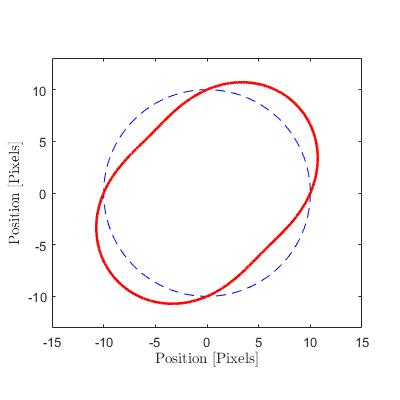
\includegraphics[width=\textwidth]{speckleradius02.jpg}
% %         \caption{$a=0$, $b=2$}
% %         % \label{fig: specklerad 1}
% %     \end{subfigure}
% %     ~ %add desired spacing between images, e. g. ~, \quad, \qquad, \hfill etc. 
% %       %(or a blank line to force the subfigure onto a new line)
% %     \begin{subfigure}[b]{0.3\textwidth}
% %         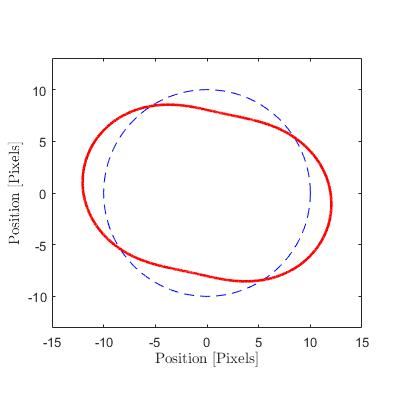
\includegraphics[width=\textwidth]{speckleradius12.jpg}
% %         \caption{$a=1$, $b=2$}
% %         % \label{fig: specklerad 2}
% %     \end{subfigure}
% %     ~ %add desired spacing between images, e. g. ~, \quad, \qquad, \hfill etc. 
% %       %(or a blank line to force the subfigure onto a new line)
% %     \begin{subfigure}[b]{0.3\textwidth}
% %         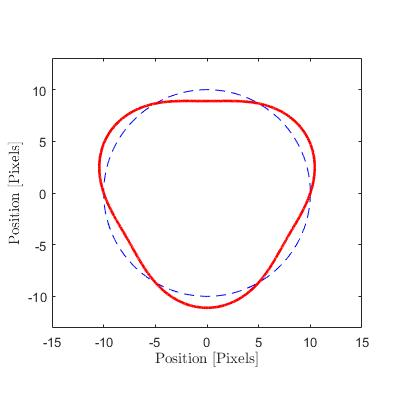
\includegraphics[width=\textwidth]{speckleradius03.jpg}
% %         \caption{$a=0$, $b=3$}
% %         % \label{fig: specklerad 3}
% %     \end{subfigure}
% %     % ~ %add desired spacing between images, e. g. ~, \quad, \qquad, \hfill etc. 
% %     %   %(or a blank line to force the subfigure onto a new line)
% %     % \begin{subfigure}[b]{0.45\textwidth}
% %     %     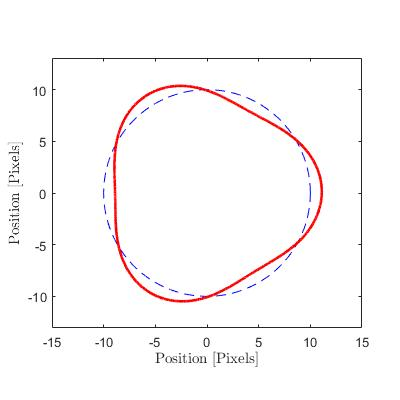
\includegraphics[width=\textwidth]{speckleradius053.jpg}
% %     %     \caption{$a=0.5$, $b=3$}
% %     %     \label{fig: specklerad 2}
% %     % \end{subfigure}
% %     \caption{The different speckle shapes created by changing variables $a$ and $b$}
% %     \label{fig: specklerad}
% % \end{figure}


% % \begin{figure}[H]
% %     \centering
% %     \begin{subfigure}[b]{0.45\textwidth}
% %     \centering
% %     \resizebox{\linewidth}{!}{
% %         % This file was created by matlab2tikz.
%
%The latest updates can be retrieved from
%  http://www.mathworks.com/matlabcentral/fileexchange/22022-matlab2tikz-matlab2tikz
%where you can also make suggestions and rate matlab2tikz.
%
\begin{tikzpicture}

\begin{axis}[%
width=3.229in,
height=2.799in,
at={(0.542in,0.757in)},
scale only axis,
xmin=-15,
xmax=15,
xlabel style={font=\color{white!15!black}},
xlabel={Position [Pixels]},
ymin=-13,
ymax=13,
ylabel style={font=\color{white!15!black}},
ylabel={Position [Pixels]},
axis background/.style={fill=white}
]
\addplot [color=blue, dashed, line width=2.0pt, forget plot]
  table[row sep=crcr]{%
10	0\\
9.97986676471884	0.634239196565645\\
9.91954812830795	1.26592453573749\\
9.81928697262707	1.8925124436041\\
9.67948701396356	2.51147987181079\\
9.50071117740946	3.12033445698487\\
9.28367933016073	3.71662455660328\\
9.02926538286621	4.29794912089172\\
8.73849377069785	4.86196736100469\\
8.41253532831181	5.40640817455598\\
8.05270257531059	5.9290792905464\\
7.66044443118978	6.42787609686539\\
7.2373403810507	6.90079011482112\\
6.78509411557132	7.34591708657533\\
6.30552667084523	7.76146464291757\\
5.80056909571198	8.14575952050336\\
5.27225467610502	8.49725429949514\\
4.72271074772683	8.81453363447582\\
4.15415013001886	9.09631995354518\\
3.56886221591872	9.34147860265107\\
2.96920375328275	9.54902241444074\\
2.35758935509427	9.71811568323542\\
1.73648177666931	9.84807753012208\\
1.10838199901011	9.93838464461254\\
0.475819158237424	9.98867339183008\\
-0.15865963834808	9.99874127673875\\
-0.792499568567885	9.96854775951942\\
-1.42314838273285	9.89821441880933\\
-2.04806668065191	9.78802446214779\\
-2.66473813690035	9.63842158559942\\
-3.27067963317421	9.45000818714669\\
-3.86345125693128	9.22354294104581\\
-4.44066612605774	8.95993774291336\\
-5	8.66025403784439\\
-5.5392006386611	8.32569854634771\\
-6.05609687137667	7.95761840530832\\
-6.54860733945285	7.55749574354258\\
-7.01474887706321	7.12694171378863\\
-7.45264449675755	6.66769000516292\\
-7.86053094742787	6.18158986220605\\
-8.23676581429833	5.67059863862771\\
-8.57983413234977	5.13677391573407\\
-8.88835448654923	4.58226521727411\\
-9.16108457432069	4.00930535406614\\
-9.39692620785908	3.42020143325669\\
-9.59492973614497	2.8173255684143\\
-9.75429786885407	2.20310532786541\\
-9.87438888676394	1.5800139597335\\
-9.95471922573085	0.950560433041829\\
-9.99496542383185	0.317279334980681\\
-9.99496542383185	-0.317279334980679\\
-9.95471922573085	-0.950560433041826\\
-9.87438888676394	-1.5800139597335\\
-9.75429786885407	-2.20310532786541\\
-9.59492973614497	-2.81732556841429\\
-9.39692620785909	-3.42020143325669\\
-9.1610845743207	-4.00930535406613\\
-8.88835448654924	-4.5822652172741\\
-8.57983413234977	-5.13677391573406\\
-8.23676581429833	-5.67059863862771\\
-7.86053094742788	-6.18158986220605\\
-7.45264449675755	-6.66769000516291\\
-7.01474887706322	-7.12694171378863\\
-6.54860733945285	-7.55749574354258\\
-6.05609687137667	-7.95761840530832\\
-5.5392006386611	-8.32569854634771\\
-5	-8.66025403784439\\
-4.44066612605774	-8.95993774291336\\
-3.86345125693129	-9.22354294104581\\
-3.27067963317422	-9.45000818714668\\
-2.66473813690035	-9.63842158559942\\
-2.04806668065191	-9.78802446214779\\
-1.42314838273285	-9.89821441880933\\
-0.792499568567888	-9.96854775951942\\
-0.158659638348076	-9.99874127673875\\
0.475819158237424	-9.98867339183008\\
1.10838199901011	-9.93838464461254\\
1.7364817766693	-9.84807753012208\\
2.35758935509427	-9.71811568323542\\
2.96920375328275	-9.54902241444074\\
3.56886221591872	-9.34147860265107\\
4.15415013001886	-9.09631995354519\\
4.72271074772682	-8.81453363447582\\
5.27225467610502	-8.49725429949514\\
5.80056909571198	-8.14575952050336\\
6.30552667084522	-7.76146464291757\\
6.78509411557132	-7.34591708657534\\
7.23734038105069	-6.90079011482113\\
7.66044443118977	-6.4278760968654\\
8.05270257531059	-5.9290792905464\\
8.41253532831181	-5.40640817455597\\
8.73849377069785	-4.86196736100469\\
9.02926538286621	-4.29794912089172\\
9.28367933016072	-3.71662455660328\\
9.50071117740946	-3.12033445698487\\
9.67948701396356	-2.51147987181079\\
9.81928697262707	-1.89251244360411\\
9.91954812830795	-1.2659245357375\\
9.97986676471884	-0.634239196565654\\
10	-2.44929359829471e-15\\
};
\addplot [color=red, line width=2.0pt, forget plot]
  table[row sep=crcr]{%
10	0\\
10.2516303315466	0.651510279471278\\
10.4554438181344	1.33431510086931\\
10.604318896481	2.04381494537044\\
10.6918192205989	2.77414378745868\\
10.712430538689	3.51830147277907\\
10.6617694622838	4.26832862178154\\
10.5367565440482	5.01551805216369\\
10.3357473497621	5.75065538578747\\
10.0586167075825	6.46428044225667\\
9.7067929896786	7.14696026017137\\
9.28324106738554	7.78956415577298\\
8.79239441668191	8.38353114289179\\
8.24003866977399	8.92112030095803\\
7.63315064521343	9.39563527989107\\
6.97969848058494	9.80161505023654\\
6.28840988092336	10.1349842108043\\
5.56851663251721	10.3931576108248\\
4.82948437461434	10.5750956771366\\
4.08073714036416	10.6813086001815\\
3.33138635441311	10.7138093619483\\
2.58997380160465	10.6760174184518\\
1.86423756552138	10.5726166127897\\
1.16090909582707	10.4093725286615\\
0.485548429911327	10.1929159394631\\
-0.157576791791381	9.93050021256156\\
-0.765564466115774	9.62974144863823\\
-1.33690100620599	9.29835073890032\\
-1.87143365858432	8.94386818679141\\
-2.37029349052879	8.57340825612721\\
-2.83577216352973	8.1934255774941\\
-3.27115727813536	7.80950958489929\\
-3.68053257074728	7.42621529259993\\
-4.06855050985515	7.04693619622938\\
-4.44018583202938	6.6738237407801\\
-4.80047924085664	6.30775609648689\\
-5.15428084024944	5.94835718375243\\
-5.50600287463076	5.59406505509498\\
-5.85939100238283	5.24224694199854\\
-6.21732264820544	4.88935657263545\\
-6.58163998929978	4.53112782428189\\
-6.95302386543638	4.16279744765514\\
-7.33091340974682	3.77934853736609\\
-7.71347452952542	3.37576566167355\\
-8.09761858476822	2.94729213329645\\
-8.47907078106847	2.48967981682131\\
-8.85248597907768	1.99942213038559\\
-9.21160789067868	1.47396150037933\\
-9.54946604497614	0.911863446190199\\
-9.85860352262787	0.312950674350446\\
-10.1313273250358	-0.321607995610914\\
-10.3599724064856	-0.989257419893456\\
-10.5371698828492	-1.68606641908767\\
-10.6561097586305	-2.40678852534522\\
-10.7107886912215	-3.14497132000728\\
-10.6962338309499	-3.89311073321693\\
-10.608694619116	-4.64284504645872\\
-10.4457955633516	-5.38518189718211\\
-10.2066443992632	-6.110750383813\\
-9.89189163929687	-6.81006945297352\\
-9.50373924665031	-7.47382315177665\\
-9.04589799113226	-8.09313306832729\\
-8.52349487949567	-8.65981837248228\\
-7.94293383865625	-9.16663430333274\\
-7.31171450189669	-9.60748071412976\\
-6.63821544529283	-9.97757335191533\\
-5.93144949014486	-10.2735718794594\\
-5.2007996813682	-10.4936601932268\\
-4.45574523572721	-10.6375762971923\\
-3.7055871028187	-10.7065907967993\\
-2.95918278327191	-10.7034349150716\\
-2.22469970271949	-10.6321807375042\\
-1.50939575925972	-10.4980780987183\\
-0.81943467102	-10.3073540704006\\
-0.159742484904775	-10.0669823409159\\
0.46608988656352	-9.78443084419707\\
1.05585490219315	-9.46739676056356\\
1.60872598781723	-9.12353844745442\\
2.12520490858389	-8.76021394801906\\
2.60702115215239	-8.38423546693316\\
3.05698729147328	-8.00164860512067\\
3.47881588542339	-7.61754422995373\\
3.87690486293644	-7.23590965812688\\
4.25609947128669	-6.85952438818595\\
4.62143971083903	-6.48990399077017\\
4.97790269647701	-6.12729400594407\\
5.33014956136865	-5.77071387219264\\
5.68228634541949	-5.41804908675045\\
6.03764779499402	-5.06618803795781\\
6.39861216094257	-4.71119832092144\\
6.76645394904112	-4.34853590685528\\
7.14124019163363	-3.9732793362219\\
7.52177422168418	-3.58038018961974\\
7.90558919803768	-3.16492049142501\\
8.28899181612991	-2.72236744119067\\
8.66715480732818	-2.2488159561629\\
9.03425504877311	-1.74120994183777\\
9.38365243848155	-1.19753397060568\\
9.70810319789112	-0.616968113660021\\
10	-2.44929359829471e-15\\
};
\draw [->] (0,0) -- (15,0);
\draw [->] (0,0) -- (8.79239441668191,8.38353114289179);
\draw[black] (3,0) arc (0: 43.6364:3);
\draw (0,0) circle[radius=1.5pt];
\fill (0,0) circle[radius=1.5pt];
\draw [dotted] (8.79239441668191,8.38353114289179) -- (10.5509,10.0602);
\draw (10.5509,10.0602) circle[radius=1.5pt];
\fill (10.5509,10.0602) circle[radius=1.5pt];
\node [below] at (0,0) {\small $(x_k,y_k)$};
\node [above] at (10.5509,10.0602) {\small $(x,y)$};
\node [above,left] at (4.3962,4.1918) {\small $R$};
\node [above,right] at (3.1144,1.6) {\small $\theta_R$};
\end{axis}
\end{tikzpicture}%
% %         }
% %         \caption{$a=0$, $b=2$, $R_{in}=15$}
% %         % \label{fig: specklerad 1}
% %     \end{subfigure}
% %     ~ %add desired spacing between images, e. g. ~, \quad, \qquad, \hfill etc. 
% %       %(or a blank line to force the subfigure onto a new line)
% %     \begin{subfigure}[b]{0.45\textwidth}
% %     \centering
% %     \resizebox{\linewidth}{!}{
% %         % This file was created by matlab2tikz.
%
%The latest updates can be retrieved from
%  http://www.mathworks.com/matlabcentral/fileexchange/22022-matlab2tikz-matlab2tikz
%where you can also make suggestions and rate matlab2tikz.
%
\begin{tikzpicture}

\begin{axis}[%
width=3.229in,
height=2.799in,
at={(0.542in,0.757in)},
scale only axis,
xmin=-15,
xmax=15,
xlabel style={font=\color{white!15!black}},
xlabel={Position [Pixels]},
ymin=-13,
ymax=13,
ylabel style={font=\color{white!15!black}},
ylabel={Position [Pixels]},
axis background/.style={fill=white}
]
\addplot [color=blue, dashed, line width=2.0pt, forget plot]
  table[row sep=crcr]{%
10	0\\
9.97986676471884	0.634239196565645\\
9.91954812830795	1.26592453573749\\
9.81928697262707	1.8925124436041\\
9.67948701396356	2.51147987181079\\
9.50071117740946	3.12033445698487\\
9.28367933016073	3.71662455660328\\
9.02926538286621	4.29794912089172\\
8.73849377069785	4.86196736100469\\
8.41253532831181	5.40640817455598\\
8.05270257531059	5.9290792905464\\
7.66044443118978	6.42787609686539\\
7.2373403810507	6.90079011482112\\
6.78509411557132	7.34591708657533\\
6.30552667084523	7.76146464291757\\
5.80056909571198	8.14575952050336\\
5.27225467610502	8.49725429949514\\
4.72271074772683	8.81453363447582\\
4.15415013001886	9.09631995354518\\
3.56886221591872	9.34147860265107\\
2.96920375328275	9.54902241444074\\
2.35758935509427	9.71811568323542\\
1.73648177666931	9.84807753012208\\
1.10838199901011	9.93838464461254\\
0.475819158237424	9.98867339183008\\
-0.15865963834808	9.99874127673875\\
-0.792499568567885	9.96854775951942\\
-1.42314838273285	9.89821441880933\\
-2.04806668065191	9.78802446214779\\
-2.66473813690035	9.63842158559942\\
-3.27067963317421	9.45000818714669\\
-3.86345125693128	9.22354294104581\\
-4.44066612605774	8.95993774291336\\
-5	8.66025403784439\\
-5.5392006386611	8.32569854634771\\
-6.05609687137667	7.95761840530832\\
-6.54860733945285	7.55749574354258\\
-7.01474887706321	7.12694171378863\\
-7.45264449675755	6.66769000516292\\
-7.86053094742787	6.18158986220605\\
-8.23676581429833	5.67059863862771\\
-8.57983413234977	5.13677391573407\\
-8.88835448654923	4.58226521727411\\
-9.16108457432069	4.00930535406614\\
-9.39692620785908	3.42020143325669\\
-9.59492973614497	2.8173255684143\\
-9.75429786885407	2.20310532786541\\
-9.87438888676394	1.5800139597335\\
-9.95471922573085	0.950560433041829\\
-9.99496542383185	0.317279334980681\\
-9.99496542383185	-0.317279334980679\\
-9.95471922573085	-0.950560433041826\\
-9.87438888676394	-1.5800139597335\\
-9.75429786885407	-2.20310532786541\\
-9.59492973614497	-2.81732556841429\\
-9.39692620785909	-3.42020143325669\\
-9.1610845743207	-4.00930535406613\\
-8.88835448654924	-4.5822652172741\\
-8.57983413234977	-5.13677391573406\\
-8.23676581429833	-5.67059863862771\\
-7.86053094742788	-6.18158986220605\\
-7.45264449675755	-6.66769000516291\\
-7.01474887706322	-7.12694171378863\\
-6.54860733945285	-7.55749574354258\\
-6.05609687137667	-7.95761840530832\\
-5.5392006386611	-8.32569854634771\\
-5	-8.66025403784439\\
-4.44066612605774	-8.95993774291336\\
-3.86345125693129	-9.22354294104581\\
-3.27067963317422	-9.45000818714668\\
-2.66473813690035	-9.63842158559942\\
-2.04806668065191	-9.78802446214779\\
-1.42314838273285	-9.89821441880933\\
-0.792499568567888	-9.96854775951942\\
-0.158659638348076	-9.99874127673875\\
0.475819158237424	-9.98867339183008\\
1.10838199901011	-9.93838464461254\\
1.7364817766693	-9.84807753012208\\
2.35758935509427	-9.71811568323542\\
2.96920375328275	-9.54902241444074\\
3.56886221591872	-9.34147860265107\\
4.15415013001886	-9.09631995354519\\
4.72271074772682	-8.81453363447582\\
5.27225467610502	-8.49725429949514\\
5.80056909571198	-8.14575952050336\\
6.30552667084522	-7.76146464291757\\
6.78509411557132	-7.34591708657534\\
7.23734038105069	-6.90079011482113\\
7.66044443118977	-6.4278760968654\\
8.05270257531059	-5.9290792905464\\
8.41253532831181	-5.40640817455597\\
8.73849377069785	-4.86196736100469\\
9.02926538286621	-4.29794912089172\\
9.28367933016072	-3.71662455660328\\
9.50071117740946	-3.12033445698487\\
9.67948701396356	-2.51147987181079\\
9.81928697262707	-1.89251244360411\\
9.91954812830795	-1.2659245357375\\
9.97986676471884	-0.634239196565654\\
10	-2.44929359829471e-15\\
};
\addplot [color=red, line width=2.0pt, forget plot]
  table[row sep=crcr]{%
11.1046281766568	0\\
11.0771441483097	0.703973226346345\\
10.9656789329765	1.39943088462464\\
10.7733516787768	2.0763933438594\\
10.5056448104267	2.72583820234666\\
10.1700900870722	3.3401796914728\\
9.77583941171281	3.91365573140201\\
9.33314744974104	4.44259761739707\\
8.85279862907822	4.92556487623244\\
8.34551452880835	5.36333652205648\\
7.8213787985914	5.7587592022121\\
7.2893155162179	6.11646196119327\\
6.75665336597118	6.44245597170568\\
6.22880243311455	6.74364503173371\\
5.70906311897024	7.02727842655093\\
5.19857815483991	7.30038153138666\\
4.69642947854193	7.56920104024603\\
4.19987242560323	7.83870085073619\\
3.70469087514291	8.11214146685792\\
3.20564924295119	8.39077050300872\\
2.69701102746786	8.67364481969655\\
2.17308938429543	8.95759644526788\\
1.628793201897	9.23734527383534\\
1.06013250262145	9.50575216371012\\
0.464649675452578	9.75419709224857\\
-0.158252113391298	9.97305902604721\\
-0.807105300397487	10.1522676517198\\
-1.47831296255141	10.2818924990381\\
-2.16622738460826	10.3527325703922\\
-2.8633677155753	10.3568695231765\\
-3.56076324473007	10.2881497392435\\
-4.24840066117915	10.1425651116608\\
-4.91574688297248	9.91850879598894\\
-5.55231408832842	9.6168901005653\\
-6.14823077175488	9.24110162064518\\
-6.6947821634137	8.79684108338915\\
-7.18488522341953	8.2917995657947\\
-7.61346753505168	7.73523618779238\\
-7.97772550955642	7.13746652844443\\
-8.27724499091711	6.50929740815941\\
-8.5139761203286	5.86144398004315\\
-8.69206362534476	5.20396606925357\\
-8.81754294154997	4.54575932857191\\
-8.89792116268879	3.89413313109511\\
-8.94166919778351	3.25450143264816\\
-8.95765721724547	2.63020547364384\\
-8.95456912814338	2.02247862636467\\
-8.94033319634457	1.43055447956158\\
-8.92160494091954	0.851909979956867\\
-8.90333512647562	0.282626715376404\\
-8.88845028220585	-0.282154212141929\\
-8.87766602696357	-0.847714322386793\\
-8.86944503440628	-1.41921157148628\\
-8.86010227099444	-2.00114234577433\\
-8.84405077059888	-2.59684761113981\\
-8.81417227161802	-3.20809634656348\\
-8.76228910716258	-3.83477440320731\\
-8.67970731313386	-4.47470012332215\\
-8.55779641330293	-5.12357986342305\\
-8.38856904220957	-5.77510751953318\\
-8.16522362187196	-6.4212028298324\\
-7.8826157122421	-7.05237423064039\\
-7.53762825296406	-7.65818394365268\\
-7.12941740975804	-8.22778629641988\\
-6.65951871564643	-8.75050545386615\\
-6.13180714349959	-9.21641607722281\\
-5.55231408832843	-9.6168901005653\\
-4.92891337655483	-9.94507484699152\\
-4.27089676956277	-10.1962719680138\\
-3.58846645535722	-10.3681929096541\\
-2.89217727537506	-10.461074390139\\
-2.19236457751579	-10.4776462199172\\
-1.49859442079569	-10.4229531395614\\
-0.819171329412442	-10.3040415974402\\
-0.160735003733455	-10.129530945486\\
0.472028412741615	-9.90909585062839\\
1.07654236409739	-9.65289233330721\\
1.6523536815656	-9.37096339384142\\
2.20100385127428	-9.07266144534952\\
2.72576669502883	-8.76612365809837\\
3.23127007737433	-8.45783290611251\\
3.72302678607963	-8.15229151134353\\
4.20690564793369	-7.85182775562243\\
4.68857785660262	-7.55654663859426\\
5.17297515182066	-7.26442714447113\\
5.66379579145509	-6.97155893152245\\
6.16309124352657	-6.67250247392222\\
6.67096138630344	-6.36074883412807\\
7.18537906972102	-6.02924892727187\\
7.70215660454114	-5.67097776050281\\
8.21505763768128	-5.27949696892641\\
8.71604852669422	-4.84947916262417\\
9.19567434260706	-4.3771601321866\\
9.64353658442337	-3.8606896692057\\
10.0488430968504	-3.30035833975183\\
10.4009959685394	-2.69868557952385\\
10.6901806544881	-2.06036344282358\\
10.9079193768256	-1.39205965779466\\
11.0475540264721	-0.702092718766141\\
11.1046281766568	-2.71984947045286e-15\\
};
\draw [->] (0,0) -- (15,0);
\draw [->] (0,0) -- (6.228802433114,6.74364503173371);
\draw[black] (3,0) arc (0:47.2727:3);
\draw (0,0) circle[radius=1.5pt];
\fill (0,0) circle[radius=1.5pt];
\draw [dotted] (6.228802433114,6.74364503173371) -- (9.3432,10.1155);
\draw (9.3432,10.1155) circle[radius=1.5pt];
\fill (9.3432,10.1155) circle[radius=1.5pt];
\node [below] at (0,0) {\small $(x_k,y_k)$};
\node [above] at (9.3432,10.1155) {\small $(x,y)$};
\node [above,left] at (3.1144,3.3718) {\small $R$};
\node [above,right] at (3.1144,1.6) {\small $\theta_R$};
\end{axis}

\end{tikzpicture}%
% %         }
% %         \caption{$a=0.5$, $b=3$, $R_{in}=15$}
% %         % \label{fig: specklerad 2}
% %     \end{subfigure}
% %     % \fcolorbox{black}{red}{\rule{0pt}{6pt}\rule{6pt}{0pt}}\quad Modified radius according to equation \ref{eq: speckle radius}.
% %     \caption{The different speckle shapes created by changing variables $a$ and $b$. Red indicates the modified radius according to equation \ref{eq: speckle radius} and blue indicates the base radius $\frac{2R_{in}}{3}$.}
% %     \label{fig: specklerad}
% % \end{figure}


% % \begin{figure}[H]
% % \begin{tikzpicture}
% %   \draw [->] (0,0) -- (9,0);
% %   \draw [->] (0,0) -- (0,5);
% %   % \draw [thick] (0,3) to [out=-60,in=-135] (8,4);
% %   \draw[red, ultra thick, domain=0:8] plot (\x, {((\x-4.5)/3)^2+0.5});
% %   \node [below] at (0,0) {\tiny $\alpha_0$};
% %   \node [below] at (8,0) {\tiny $\alpha_1$};
% %   \node [below] at (3.05,0) {\tiny $\alpha_2$};
% %   \node [below] at (4.94,0) {\tiny $\alpha_3$};
% %   \draw [-] (3.05,-0.1) -- (3.05,0.731769038890291);
% %   \draw [-] (4.94,-0.1) -- (4.94,0.521930836668256);
% %   \draw [-] (0,0) -- (0,-0.1);
% %   \draw [-] (8,-0.1) -- (8,1.861111111111111);
% %   \node [left,rotate=90] at (-0.3,4) {\small Correlation Coefficient};
% %   \node [below] at (4.5,-0.7) {\small Step size in search direction};
% %   \node [above] at (3.05,0.8) {\tiny $C_2$};
% %   \node [above] at (4.94,0.6) {\tiny $C_3$};
% % \end{tikzpicture}
% % \caption{First iteration of golden section search method}
% % \label{fig: golden section 1dfs}
% % \end{figure}


% % % This file was created by matlab2tikz.
%
%The latest updates can be retrieved from
%  http://www.mathworks.com/matlabcentral/fileexchange/22022-matlab2tikz-matlab2tikz
%where you can also make suggestions and rate matlab2tikz.
%
\begin{tikzpicture}

\begin{axis}[%
width=2.229in,
height=1.799in,
at={(0.542in,0.757in)},
scale only axis,
xmin=-15,
xmax=15,
xlabel style={font=\color{white!15!black}},
xlabel={Position [Pixels]},
ymin=-13,
ymax=13,
ylabel style={font=\color{white!15!black}},
ylabel={Position [Pixels]},
axis background/.style={fill=white}
]
\addplot [color=blue, dashed, forget plot]
  table[row sep=crcr]{%
10	0\\
9.97986676471884	0.634239196565645\\
9.91954812830795	1.26592453573749\\
9.81928697262707	1.8925124436041\\
9.67948701396356	2.51147987181079\\
9.50071117740946	3.12033445698487\\
9.28367933016073	3.71662455660328\\
9.02926538286621	4.29794912089172\\
8.73849377069785	4.86196736100469\\
8.41253532831181	5.40640817455598\\
8.05270257531059	5.9290792905464\\
7.66044443118978	6.42787609686539\\
7.2373403810507	6.90079011482112\\
6.78509411557132	7.34591708657533\\
6.30552667084523	7.76146464291757\\
5.80056909571198	8.14575952050336\\
5.27225467610502	8.49725429949514\\
4.72271074772683	8.81453363447582\\
4.15415013001886	9.09631995354518\\
3.56886221591872	9.34147860265107\\
2.96920375328275	9.54902241444074\\
2.35758935509427	9.71811568323542\\
1.73648177666931	9.84807753012208\\
1.10838199901011	9.93838464461254\\
0.475819158237424	9.98867339183008\\
-0.15865963834808	9.99874127673875\\
-0.792499568567885	9.96854775951942\\
-1.42314838273285	9.89821441880933\\
-2.04806668065191	9.78802446214779\\
-2.66473813690035	9.63842158559942\\
-3.27067963317421	9.45000818714669\\
-3.86345125693128	9.22354294104581\\
-4.44066612605774	8.95993774291336\\
-5	8.66025403784439\\
-5.5392006386611	8.32569854634771\\
-6.05609687137667	7.95761840530832\\
-6.54860733945285	7.55749574354258\\
-7.01474887706321	7.12694171378863\\
-7.45264449675755	6.66769000516292\\
-7.86053094742787	6.18158986220605\\
-8.23676581429833	5.67059863862771\\
-8.57983413234977	5.13677391573407\\
-8.88835448654923	4.58226521727411\\
-9.16108457432069	4.00930535406614\\
-9.39692620785908	3.42020143325669\\
-9.59492973614497	2.8173255684143\\
-9.75429786885407	2.20310532786541\\
-9.87438888676394	1.5800139597335\\
-9.95471922573085	0.950560433041829\\
-9.99496542383185	0.317279334980681\\
-9.99496542383185	-0.317279334980679\\
-9.95471922573085	-0.950560433041826\\
-9.87438888676394	-1.5800139597335\\
-9.75429786885407	-2.20310532786541\\
-9.59492973614497	-2.81732556841429\\
-9.39692620785909	-3.42020143325669\\
-9.1610845743207	-4.00930535406613\\
-8.88835448654924	-4.5822652172741\\
-8.57983413234977	-5.13677391573406\\
-8.23676581429833	-5.67059863862771\\
-7.86053094742788	-6.18158986220605\\
-7.45264449675755	-6.66769000516291\\
-7.01474887706322	-7.12694171378863\\
-6.54860733945285	-7.55749574354258\\
-6.05609687137667	-7.95761840530832\\
-5.5392006386611	-8.32569854634771\\
-5	-8.66025403784439\\
-4.44066612605774	-8.95993774291336\\
-3.86345125693129	-9.22354294104581\\
-3.27067963317422	-9.45000818714668\\
-2.66473813690035	-9.63842158559942\\
-2.04806668065191	-9.78802446214779\\
-1.42314838273285	-9.89821441880933\\
-0.792499568567888	-9.96854775951942\\
-0.158659638348076	-9.99874127673875\\
0.475819158237424	-9.98867339183008\\
1.10838199901011	-9.93838464461254\\
1.7364817766693	-9.84807753012208\\
2.35758935509427	-9.71811568323542\\
2.96920375328275	-9.54902241444074\\
3.56886221591872	-9.34147860265107\\
4.15415013001886	-9.09631995354519\\
4.72271074772682	-8.81453363447582\\
5.27225467610502	-8.49725429949514\\
5.80056909571198	-8.14575952050336\\
6.30552667084522	-7.76146464291757\\
6.78509411557132	-7.34591708657534\\
7.23734038105069	-6.90079011482113\\
7.66044443118977	-6.4278760968654\\
8.05270257531059	-5.9290792905464\\
8.41253532831181	-5.40640817455597\\
8.73849377069785	-4.86196736100469\\
9.02926538286621	-4.29794912089172\\
9.28367933016072	-3.71662455660328\\
9.50071117740946	-3.12033445698487\\
9.67948701396356	-2.51147987181079\\
9.81928697262707	-1.89251244360411\\
9.91954812830795	-1.2659245357375\\
9.97986676471884	-0.634239196565654\\
10	-2.44929359829471e-15\\
};
\addplot [color=red, line width=2.0pt, forget plot]
  table[row sep=crcr]{%
11.1046281766568	0\\
11.0771441483097	0.703973226346345\\
10.9656789329765	1.39943088462464\\
10.7733516787768	2.0763933438594\\
10.5056448104267	2.72583820234666\\
10.1700900870722	3.3401796914728\\
9.77583941171281	3.91365573140201\\
9.33314744974104	4.44259761739707\\
8.85279862907822	4.92556487623244\\
8.34551452880835	5.36333652205648\\
7.8213787985914	5.7587592022121\\
7.2893155162179	6.11646196119327\\
6.75665336597118	6.44245597170568\\
6.22880243311455	6.74364503173371\\
5.70906311897024	7.02727842655093\\
5.19857815483991	7.30038153138666\\
4.69642947854193	7.56920104024603\\
4.19987242560323	7.83870085073619\\
3.70469087514291	8.11214146685792\\
3.20564924295119	8.39077050300872\\
2.69701102746786	8.67364481969655\\
2.17308938429543	8.95759644526788\\
1.628793201897	9.23734527383534\\
1.06013250262145	9.50575216371012\\
0.464649675452578	9.75419709224857\\
-0.158252113391298	9.97305902604721\\
-0.807105300397487	10.1522676517198\\
-1.47831296255141	10.2818924990381\\
-2.16622738460826	10.3527325703922\\
-2.8633677155753	10.3568695231765\\
-3.56076324473007	10.2881497392435\\
-4.24840066117915	10.1425651116608\\
-4.91574688297248	9.91850879598894\\
-5.55231408832842	9.6168901005653\\
-6.14823077175488	9.24110162064518\\
-6.6947821634137	8.79684108338915\\
-7.18488522341953	8.2917995657947\\
-7.61346753505168	7.73523618779238\\
-7.97772550955642	7.13746652844443\\
-8.27724499091711	6.50929740815941\\
-8.5139761203286	5.86144398004315\\
-8.69206362534476	5.20396606925357\\
-8.81754294154997	4.54575932857191\\
-8.89792116268879	3.89413313109511\\
-8.94166919778351	3.25450143264816\\
-8.95765721724547	2.63020547364384\\
-8.95456912814338	2.02247862636467\\
-8.94033319634457	1.43055447956158\\
-8.92160494091954	0.851909979956867\\
-8.90333512647562	0.282626715376404\\
-8.88845028220585	-0.282154212141929\\
-8.87766602696357	-0.847714322386793\\
-8.86944503440628	-1.41921157148628\\
-8.86010227099444	-2.00114234577433\\
-8.84405077059888	-2.59684761113981\\
-8.81417227161802	-3.20809634656348\\
-8.76228910716258	-3.83477440320731\\
-8.67970731313386	-4.47470012332215\\
-8.55779641330293	-5.12357986342305\\
-8.38856904220957	-5.77510751953318\\
-8.16522362187196	-6.4212028298324\\
-7.8826157122421	-7.05237423064039\\
-7.53762825296406	-7.65818394365268\\
-7.12941740975804	-8.22778629641988\\
-6.65951871564643	-8.75050545386615\\
-6.13180714349959	-9.21641607722281\\
-5.55231408832843	-9.6168901005653\\
-4.92891337655483	-9.94507484699152\\
-4.27089676956277	-10.1962719680138\\
-3.58846645535722	-10.3681929096541\\
-2.89217727537506	-10.461074390139\\
-2.19236457751579	-10.4776462199172\\
-1.49859442079569	-10.4229531395614\\
-0.819171329412442	-10.3040415974402\\
-0.160735003733455	-10.129530945486\\
0.472028412741615	-9.90909585062839\\
1.07654236409739	-9.65289233330721\\
1.6523536815656	-9.37096339384142\\
2.20100385127428	-9.07266144534952\\
2.72576669502883	-8.76612365809837\\
3.23127007737433	-8.45783290611251\\
3.72302678607963	-8.15229151134353\\
4.20690564793369	-7.85182775562243\\
4.68857785660262	-7.55654663859426\\
5.17297515182066	-7.26442714447113\\
5.66379579145509	-6.97155893152245\\
6.16309124352657	-6.67250247392222\\
6.67096138630344	-6.36074883412807\\
7.18537906972102	-6.02924892727187\\
7.70215660454114	-5.67097776050281\\
8.21505763768128	-5.27949696892641\\
8.71604852669422	-4.84947916262417\\
9.19567434260706	-4.3771601321866\\
9.64353658442337	-3.8606896692057\\
10.0488430968504	-3.30035833975183\\
10.4009959685394	-2.69868557952385\\
10.6901806544881	-2.06036344282358\\
10.9079193768256	-1.39205965779466\\
11.0475540264721	-0.702092718766141\\
11.1046281766568	-2.71984947045286e-15\\
};
\end{axis}
\end{tikzpicture}%

% The amplitude of the sinusoid is set to a third of the desired speckle size and it is altered according to the function $f_{amp}$ which is a function of the frequency. It was found that when the frequency of the sinusoid increased the resulting speckle would exhibit a star shape, as in Figure \ref{fig: star speckle 1a}, which is undesirable. This function, $f_{amp}$, corrects for this by decreasing the amplitude of the sinusoid as the frequency increases.

% \begin{figure}[H]
%     \centering
%     \begin{subfigure}[b]{0.45\textwidth}
%         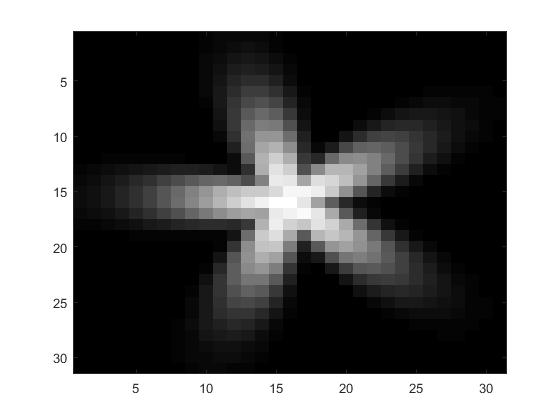
\includegraphics[width=\textwidth]{star_speckle.jpg}
%         \caption{Undesired star shaped speckle}
%         \label{fig: star speckle 1a}
%     \end{subfigure}
%     ~ %add desired spacing between images, e. g. ~, \quad, \qquad, \hfill etc. 
%       %(or a blank line to force the subfigure onto a new line)
%     \begin{subfigure}[b]{0.45\textwidth}
%         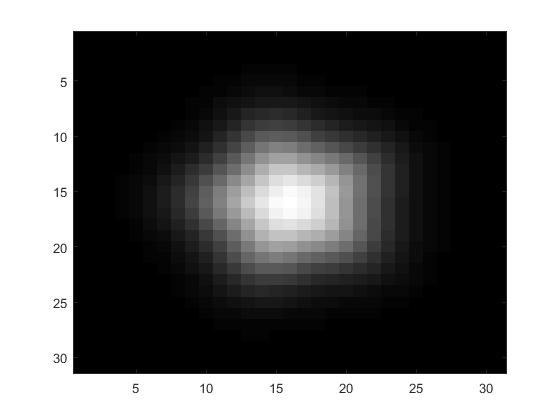
\includegraphics[width=\textwidth]{speckle_5.jpg}
%         \caption{Star shaped speckle corrected}
%         % \label{fig: speckle 2a}
%     \end{subfigure}
%     \caption{The effect of the function $f_{amp}$ for higher frequencies}
%     \label{fig: star speckle}
% \end{figure}

% Therefore the final speckle function is obtained by substituting Equation \ref{eq: speckle radius} into Equation \ref{eq: single speckle} to obtain
% \begin{equation}
%   f_{sp}(x,y) = \sum_{k=1}^{s} I_k \exp{ \left[ -\frac{ \left( x-x_k \right) ^2 + \left( y-y_k \right) ^2}{\left( \frac{R_{in}}{3} \times f_{amp}(b) \times \sin \left( \left( \arctan{ \left( \frac{y-y_k}{x-x_k} \right) } +a_k \right) \times b_k \right) +\frac{2R_{in}}{3} \right)^2} \right] }
% \end{equation}

% \subsubsection{Deformed images}
% At this point the method for generating the reference image is fully outlined however deformed versions of this reference image are required to perform correlation on. A displacement field is required for this purpose. A displacement field consists of two 2D functions which describe the displacement in the x and y directions of the speckle pattern throughout the image, these are $f_{ux}(x,y)$ and $f_{uy}(x,y)$ respectively. 

% Although this displacement field describes how the speckle pattern should deform it does not have to be applied to the speckle pattern directly to achieve this. Instead the inverse of the displacement field (displacement in the direction opposite to what the displacement field describes) can be applied to the grid of pixel centre locations. In doing so the locations where the speckle pattern is sampled change thereby simulating the deformation between the images that is described by the displacement field.

% It is for this reason that the speckle function is created to be continuous so that no interpolation is needed to determine the light intensity at these new pixel locations.

% Therefore if the reference speckle image is created by sampling the speckle function $f_{sp}$ at pixel locations $(\bm{x},\bm{y})$ like so \todo{not formal enough} 
% \begin{equation}
%   \bm{F_{speckle}} = f_{sp}(\bm{x},\bm{y}) 
% \end{equation}
% then the deformed image is obtain as
% \begin{equation}
%   \bm{G_{speckle}} = f_{sp}(\bm{x}-f_{ux}(\bm{x},\bm{y}),\bm{y}-f_{uy}(\bm{x},\bm{y})) 
% \end{equation}

% The grid of pixel centre locations are displaced as above prior to performing stochastic sampling.

% \subsubsection{Code explanation}
% First the function creates two matrices of points (X and Y) that correspond to the centre location of the pixels which are to be generated. Thereafter between lines 17 and 33 matrices of jittered displacements are created for the purpose of stochastic sampling. By adding these matrices to a pixel centre location a grid of jittered positions that fall within the fillfactor area of the pixel are obtained. Thus the same jittered grid is used for each pixel in order to improve efficiency of the algorithm.

% Thereafter the function defines the speckle pattern by assigning values to the properties of each speckle. First the vector of speckle sizes is converted from units of pixels to the units used in the displacement function hereafter referred to as displacement units (line 40). It was originally in units of pixels because for a good image the speckle sizes must be proportional to the subset size which is in units of pixels. The position of the speckles are then defined, in displacement units, at random locations that fall within the range of the image (lines 42-43). The light intensity at the centre of each speckle is then randomly defined to fall in the range between 0.5 and 1 where 1 is white and 0 is black (line 44).

% The for loop starting at line 54 saves the details of every speckle. First a random phase shift (a) and frequency (b) are defined. The phase shift falls in the range between $0$ and $2 \pi$ so that the speckle has equal chance of being rotated to any angle. The frequency is defined such that between 1 and 5 complete cycles of the sinusoid occur within one full revolution of the radius angle. Note that the frequency is only permitted to be whole numbers so that the radius of the speckle is continuous. The five possible speckle shapes resulting from the five different frequencies are illustrated in Figure \ref{fig: speckle shapes}. The amplitude (c) is then determined based on the frequency using the function on line 48. The base radius (d), x and y positions (Xk and Yk) and the light intensity (I0) are then all saved.

% \begin{figure}[H]
%     \centering
%     \begin{subfigure}[b]{0.3\textwidth}
%         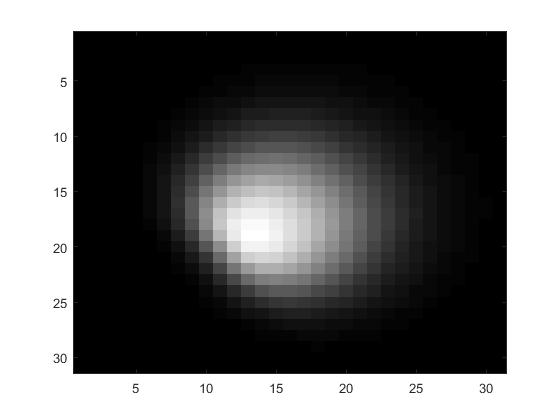
\includegraphics[width=\textwidth]{speckle_1.jpg}
%         \caption{b=1}
%         % \label{fig: speckle 1}
%     \end{subfigure}
%     ~ %add desired spacing between images, e. g. ~, \quad, \qquad, \hfill etc. 
%       %(or a blank line to force the subfigure onto a new line)
%     \begin{subfigure}[b]{0.3\textwidth}
%         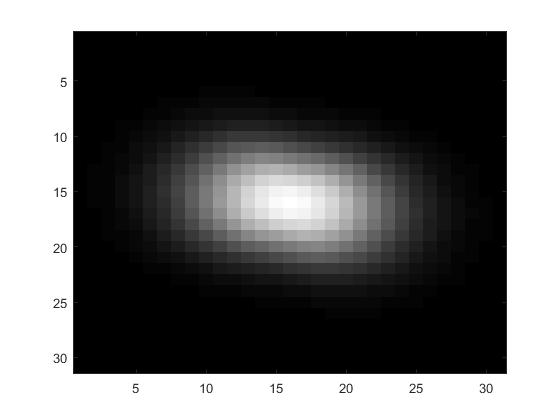
\includegraphics[width=\textwidth]{speckle_2.jpg}
%         \caption{b=2}
%         % \label{fig: speckle 2}
%     \end{subfigure}
%     ~ %add desired spacing between images, e. g. ~, \quad, \qquad, \hfill etc. 
%     %(or a blank line to force the subfigure onto a new line)
%     \begin{subfigure}[b]{0.3\textwidth}
%         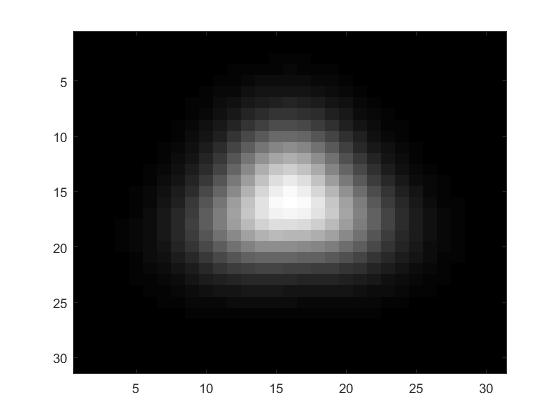
\includegraphics[width=\textwidth]{speckle_3.jpg}
%         \caption{b=3}
%         % \label{fig: speckle 3}
%     \end{subfigure}
%      ~ %add desired spacing between images, e. g. ~, \quad, \qquad, \hfill etc. 
%     %(or a blank line to force the subfigure onto a new line)
%     \begin{subfigure}[b]{0.3\textwidth}
%         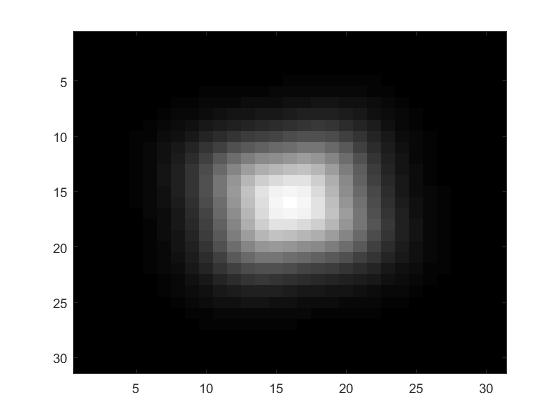
\includegraphics[width=\textwidth]{speckle_4.jpg}
%         \caption{b=4}
%         % \label{fig: speckle 4}
%     \end{subfigure}
%     ~ %add desired spacing between images, e. g. ~, \quad, \qquad, \hfill etc. 
%     %(or a blank line to force the subfigure onto a new line)
%     \begin{subfigure}[b]{0.3\textwidth}
%         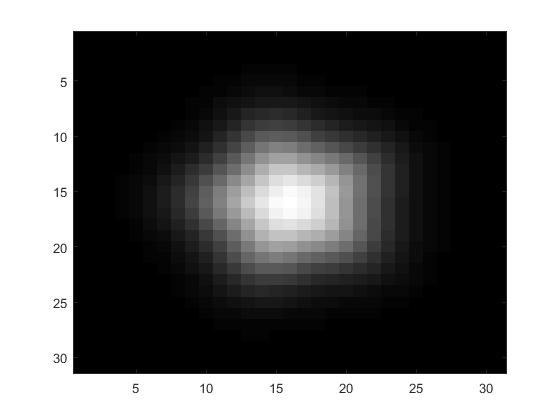
\includegraphics[width=\textwidth]{speckle_5.jpg}
%         \caption{b=5}
%         % \label{fig: speckle 5}
%     \end{subfigure}
%     \caption{Speckle shapes as a result of the frequency (b) of the sinusoid}\label{fig: speckle shapes}
% \end{figure}

% Stochastic sampling relies upon using the average of the sampled locations for each pixel to determine that pixels light intensity value. A Gaussian weighted average (H at line 72) is used to do this in order to allow the sampled locations closer to the pixel centre to have a greater influence on the light intensity value. 

% With all the necessary variables defined the calculation of light intensity values at specific locations in the image can commence. This is done between lines 79 and 154. First the locations where the speckle function is to be sampled are defined between lines 94-100. For the reference image (imageCount=1) the points to be evaluated (Xin and Yin) are determined by adding the row vectors of jittered displacements (xxgrid and yygrid) to the column vectors of x and y pixel centre locations (X and Y).

% For the case of the deformed image the points to be evaluated are determined by subtracting the displacement at that point (fux and fuy functions) from the group of x and y positions (X and Y) and then adding the jittered displacement row vectors (xxgrid and yygrid). 

% % In doing so the pixel point is displaced in the opposite direction compared to what is described by the displacement function. This is done because displacement of the speckle pattern according the the displacement function while holding the pixel locations constant is equivalent to displacing the pixel locations in the opposite direction to the displacement function and holding the speckle pattern constant. 

% Evaluating the light intensity at a location in the image involves five steps. First for each sampling location the distance between it and all the speckle centres needs to be determined (line 108-109).  

% % The second step involves determining the angles between the imaginary lines, that pass through the speckle centres and the location under consideration, and the x-axis.
% The second step involves determining the radius angle for each speckle such that the sampling location lies along the radius line at this angle. This is done by applying Matlab's atan2 function to the x and y distances "X1" and "Y1". The third step involves determining the radius of each speckle at these radius angles. This is done by applying the phase shifts and frequency changes to the angles, taking the sin of the angles, multiplying them by their respective amplitudes and adding the base radii. This results in the matrix "sins1" (line 114-117). 

% The fourth step requires determining how much each speckle contributes to the sampling location. This is done by first determining the squared distance between the speckle centre and the location under consideration which is done using Pythagoras to get "M" (line 123-127). The contribution of each speckle is determined by taking the exponent of the negative of this distance (M) divided by the speckle radius squared (line 132). This results in the matrix "speckleContribution".

% In the final step the overall light intensity at the sampling location can be determined by multiplying the contribution of each speckle by its light intensity to get "Image\_temp".

% The light intensities are then rearranged to that the light intensities that contribute to the same pixel are grouped together (line 137-140). These groups of light intensities are then multiplied by their corresponding weighted average and then summed to obtain the light intensities for pixels of the image (line 143). 

% Once both of the image matrices have been fully populated their light intensities are quantized according to 12 bit quantisation to be consistent with the cameras used during experimental tests (line 159-160). This is done using Matlab's imquantize function (line 169).

% Since sampling the speckle function (line 83-153) involves a large number of simple operations it was discovered that it runs faster on a graphics processing unit (GPU). It is for this reason that Matlab's reshape function is often used to vectorise matrices so that the sampling process can be performed using matrix operations. In doing so multiple locations in the image are sampled simultaneously resulting in faster computation of the synthetic images. 

% However GPUs have a limited amount of memory and so the number of points that can be evaluated simultaneously is limited. To cope with this the points to be evaluated are divided into groups so that the memory required to evaluate each group is less than what is available. This is the purpose of the for loop starting at line 83. 

% The number of groups is determined by dividing the overall memory requirements of the total image by the memory that is available. Using a simplified approach the total memory requirements of the image is the number of pixels in the image times the number of points that need to be evaluated for each pixel times the number of speckles. This is divided by the available memory which is 44567000 for the computer used during this project (line 67). If a different computer is used this value should be adjusted. %Note that these memory values are relative values and have no units.





\subsection{Displacement fields}
A variety of displacement fields have been used to create synthetic image sets. The first two give theoretical displacement fields for a plate of material in the vicinity of a stress concentration which causes complex displacement fields. The final displacement field is designed to test the limitations of the framework so that the point at which the proposed framework breaks down can be compared to that of commercial software. (NOTE: still need to design this displacement field and present subsequent discussion of it.)

The displacement field equations are given as a function of the sampling point, $(x,y)$, and an additional parameter which controls the severity of the displacement field. The reason for this is so that an image set containing multiple deformed images, of increasing deformation, can be created by altering this variable.

% The DIC framework presented in this project is focused on material science. As such the first two displacement fields used approximate displacements that a plate of material would experience in the presence of a stress concentration. The purpose of this is so that the accuracy and precision of the framework with regards to realistic material deformation can be evaluated. These displacement fields are also closely linked to the displacements expected from the specimens used for experimental validation in Chapter \ref{ch: experimental tests}.

% The final displacement field is designed to test the limitations of the framework so that the point at which the proposed framework breaks down can be compared to that of commercial software. (NOTE: still need to design this displacement field and present subsequent discussion of it.)

\subsubsection{Plate with hole}
\label{sec: plate hole}
The displacement field experienced by an infinite plate of material containing a hole subjected to stress $S$, shown in Figure \ref{fig: plate with hole}, has been calculated in Appendix \ref{ap: plate hole}. The final form of these displacement fields is given as 
\begin{align}
  f_u(x,y,S) &= \frac{S\,a}{8\,\mu } \bigg[\frac{2\,a}{\sqrt{x^2+y^2}} \left(\cos\left(3\,\text{atan2}(y,x) \right)+\cos\left( \text{atan2}(y,x) \right)\,\left(k+1\right)\right) \nonumber \\ &-\frac{2\,a^3}{\left( \sqrt{x^2+y^2} \right) ^3} \cos\left(3\, \text{atan2}(y,x) \right)+\frac{\sqrt{x^2+y^2}}{a} \cos\left( \text{atan2}(y,x) \right)\,\left(k+1\right)  \bigg] \\
  f_v(x,y,S) &= \frac{S\,a}{8\,\mu } \bigg[\frac{2\,a}{\sqrt{x^2+y^2}} \left(\sin\left(3\, \text{atan2}(y,x) \right)-\sin\left( \text{atan2}(y,x) \right)\,\left(k-1\right)\right) \nonumber \\ &-\frac{2\,a^3}{ \left( \sqrt{x^2+y^2} \right)^3} \sin\left(3\, \text{atan2}(y,x) \right) +\frac{\sqrt{x^2+y^2}}{a} \sin\left( \text{atan2}(y,x) \right)\,\left(k-3\right)  \bigg]
\end{align}
Note that atan2 is a Matlab function which computes the arctan of a vector and returns the angle corresponding to the correct quadrant within which that vector lies. These displacement fields are only valid for x and y positions that lie outside of the radius of the hole. Here $\mu$ is the shear modulus and $k$ is Kolosov's constant. The values for the shear modulus and Kolosov's constant are determined from the elastic modulus, $E$, and Poisson's ratio, $v$, under the assumption of plane stress as
\begin{equation}
\label{eq: shear kolosovs}
   \mu=\frac{E}{2(1+v)} \quad \text{and} \quad k=\frac{3-v}{1+v}.
\end{equation} 



% Interesting displacement fields often occur in the vicinity of a stress concentration. A hole in a plate is a specimen geometry that causes a such a stress concentration. This specimen geometry was chosen because equations can be derived that describe the displacement the specimen experiences when subjected to a normal stress $S$ as illustrated in Figure \ref{fig: plate with hole}. These equations are derived using the Airy stress function as done by Barber in \cite{barber2002solid}. The Airy stress function is a method of using equilibrium equations and boundary conditions of the specimen to solve for the two-dimensional stress and displacement fields experienced by the specimen.

\begin{figure}[H]
\centering
\begin{tikzpicture}[scale=1]  
    \draw [line width=0.4mm,-] (0,0) -- (5,0) -- (5,-5) -- (0,-5) -- (0,0);
    \draw [line width=0.4mm,black] (2.5,-2.5) circle (1cm);
    \draw [line width=0.15mm,->] (2.5,-2.5) -- (4.5,-2.5);
    \draw [line width=0.15mm,->] (2.5,-2.5) -- (2.5,-0.5);
    \draw [line width=0.25mm,->] (2.5,-2.5) -- (1.633974596215561,-2);
    \draw [line width=0.25mm,->] (2.5,-2.5) -- (4.5,-0.5);
    \draw [line width=0.25mm,black] (4,-2.5) arc (0:45:1.5);
    \node [right] at (4.5,-2.5) {\footnotesize $x$};
    \node [above] at (2.5,-0.5) {\footnotesize $y$};
    \node [above,right] at (4.5,-0.5) {\footnotesize $r$};
    \node [above,right] at (3.885819298766930,-1.925974851452365) {\footnotesize $\theta$};
    \node [above] at (2.066987298107780,-2.250000000000000) {\footnotesize $a$};
    \draw [->] (0,-0.5) -- (-0.5,-0.5);
    \draw [->] (0,-1) -- (-0.5,-1);
    \draw [->] (0,-1.5) -- (-0.5,-1.5);
    \draw [->] (0,-2) -- (-0.5,-2);
    \draw [->] (0,-2.5) -- (-0.5,-2.5);
    \draw [->] (0,-3) -- (-0.5,-3);
    \draw [->] (0,-3.5) -- (-0.5,-3.5);
    \draw [->] (0,-4) -- (-0.5,-4);
    \draw [->] (0,-4.5) -- (-0.5,-4.5);

    \draw [->] (5,-0.5) -- (5.5,-0.5);
    \draw [->] (5,-1.5) -- (5.5,-1.5);
    \draw [->] (5,-2.5) -- (5.5,-2.5);
    \draw [->] (5,-3.5) -- (5.5,-3.5);
    \draw [->] (5,-4.5) -- (5.5,-4.5);
    \draw [->] (5,-1) -- (5.5,-1);
    \draw [->] (5,-2) -- (5.5,-2);
    \draw [->] (5,-3) -- (5.5,-3);
    \draw [->] (5,-4) -- (5.5,-4);
    \node [left] at (-0.5,-2.5) {\footnotesize $S$};
    \node [right] at (5.5,-2.5) {\footnotesize $S$};
\end{tikzpicture}
\caption{Plate with hole}
\label{fig: plate with hole}
\end{figure}

% For the case of a large plate with a circular hole in it experiencing a uniform normal stress, $S$, in the x direction the stress function in terms of polar coordinates is
% \begin{equation}
%   \phi = \frac{Sr^2}{4} - \frac{Sr^2 \cos(2 \theta)}{4} -\frac{Sa^2}{2} + \frac{Sa^2}{2} \cos(2 \theta) - \frac{Sa^4}{4r^2} \cos(2 \theta)
% \end{equation}
% where $a$ is the radius of the hole.

% The displacement equations are derived from this by substituting in the appropriate displacement components from the Michell solution \cite{michell1899direct}. These components are tabulated in \cite{barber2002solid} (should I say this?) \todo{keep this in or not?}. After substitution the displacement equations become
% \begin{align}
%   u_r(r,\theta) &= \frac{1}{2 \mu} \biggl \{ \frac{S}{4} \left[ (k-1)r \right]-\frac{S}{4} \left[ -2r\cos(2\theta) \right] -\frac{Sa^2}{2} \left[ -\frac{1}{r} \right]  \\ 
%   &+\frac{Sa^2}{2}\left[ \frac{k+1}{r} \cos(2 \theta)\right] - \frac{Sa^4}{4}\left[ \frac{2}{r^3} \cos(2 \theta) \right] \biggr\} \nonumber \\
%   u_{\theta}(r,\theta) &= \frac{1}{2 \mu} \left\{ -\frac{S}{4} \left[ 2r \sin(2 \theta) \right] + \frac{Sa^2}{2}\left[ -\frac{k-1}{r} \sin(2 \theta) \right]- \frac{Sa^4}{4} \left[ \frac{2}{r^3} \sin(2 \theta) \right] \right\}
% \end{align}
% % \begin{align}
% %   2 \mu u_r &= \frac{S}{4} \left[ (k-1)r \right]-\frac{S}{4} \left[ -2r\cos(2\theta) \right] -\frac{Sa^2}{2} \left[ -\frac{1}{r} \right] +\frac{Sa^2}{2}\left[ \frac{k+1}{r} \cos(2 \theta)\right] - \frac{Sa^4}{4}\left[ \frac{2}{r^3} \cos(2 \theta) \right] \\
% %   2 \mu u_{\theta} &= -\frac{S}{4} \left[ 2r \sin(2 \theta) \right] + \frac{Sa^2}{2}\left[ -\frac{k-1}{r} \sin(2 \theta) \right]- \frac{Sa^4}{4} \left[ \frac{2}{r^3} \sin(2 \theta) \right]
% % \end{align}
% where the substituted displacement components are indicated by square brackets. Here $u_r$ is radial displacement, $u_{\theta}$ is angular displacement, $\mu$ is the shear modulus and $k$ is Kolosov's constant. These equations can be converted to describe the displacement in terms of cartesian coordinates using the following equations
% \begin{align}
%   u_x(r,\theta) = u_r(r,\theta) \cos(\theta) - u_{\theta}(r,\theta) \sin(\theta) \\
%   u_y(r,\theta) = u_r(r,\theta) \sin(\theta) + u_{\theta}(r,\theta) \cos(\theta) \\
%   \text{where} \quad r=\sqrt{x^2+y^2} \quad \text{and} \quad \theta = \text{atan2} (y,x). \label{eq: pol2cart}
% \end{align}



% % Further substitution of $\frac{E}{2(1+v)}$ for $\mu$ and $\frac{3-v}{1+v}$ for $k$ (plane stress condition), where $E$ is the elastic modulus and $v$ is Poisson's ratio, gives
% % \begin{align}
% %   u_r(r,\theta) &= \frac{Sr \cos(2 \theta)}{2E} \left[ 1+v+4\frac{a^2}{r^2} - (1+v)\frac{a^4}{r^4} \right] + \frac{Sr}{2E} \left[ 1-v+(1+v)\frac{a^2}{r^2} \right] \\
% %   u_{\theta}(r,\theta) &= - \frac{Sr \sin(2 \theta)}{2E}\left[ 1+v+2(1-v)\frac{a^2}{r^2} + (1+v)\frac{a^4}{r^4} \right]
% % \end{align}

% % These equations can be converted to describe the displacement in terms of cartesian coordinates using the following equations

% Note that atan2 is a Matlab function which computes the arctan of a vector and returns the angle corresponding to the correct quadrant within which that vector lies. The displacement equations in cartesian coordinates become
% % \begin{align}
% %   u_x(r,\theta) &= \frac{S\,a}{8\,\mu }\left(\frac{2\,a}{r} \left(\cos\left(3\,t\right)+\cos\left(t\right)\,\left(k+1\right)\right)-\frac{2\,a^3}{r^3} \cos\left(3\,t\right)+\frac{r}{a} \cos\left(t\right)\,\left(k+1\right) \right)\\
% %   u_y(r,\theta) &= \frac{S\,a}{8\,\mu }\left(\frac{2\,a}{r} \left(\sin\left(3\,t\right)-\sin\left(t\right)\,\left(k-1\right)\right) -\frac{2\,a^3}{r^3} \sin\left(3\,t\right) +\frac{r}{a} \sin\left(t\right)\,\left(k-3\right) \right)
% % \end{align}
% % Making use of the knowledge that $r=\sqrt{x^2+y^2}$ and $\theta = \text{atan2} (y,x)$ the displacement equations can be rewritten in terms of only cartesian coordinates

% \begin{align}
%   u_x(x,y) &= \frac{S\,a}{8\,\mu } \bigg[\frac{2\,a}{\sqrt{x^2+y^2}} \left(\cos\left(3\,\text{atan2}(y,x) \right)+\cos\left( \text{atan2}(y,x) \right)\,\left(k+1\right)\right) \nonumber \\ &-\frac{2\,a^3}{\left( \sqrt{x^2+y^2} \right) ^3} \cos\left(3\, \text{atan2}(y,x) \right)+\frac{\sqrt{x^2+y^2}}{a} \cos\left( \text{atan2}(y,x) \right)\,\left(k+1\right)  \bigg] \\
%   u_y(x,y) &= \frac{S\,a}{8\,\mu } \bigg[\frac{2\,a}{\sqrt{x^2+y^2}} \left(\sin\left(3\, \text{atan2}(y,x) \right)-\sin\left( \text{atan2}(y,x) \right)\,\left(k-1\right)\right) \nonumber \\ &-\frac{2\,a^3}{ \left( \sqrt{x^2+y^2} \right)^3} \sin\left(3\, \text{atan2}(y,x) \right) +\frac{\sqrt{x^2+y^2}}{a} \sin\left( \text{atan2}(y,x) \right)\,\left(k-3\right)  \bigg]
% \end{align}
% \todo{take this out since it is unnecessary?}
% % Note that atan2 is a Matlab function which computes the arctan of a vector and returns the angle corresponding to the correct quadrant within which that vector lies. 
% These displacement fields are only valid for x and y positions that lie outside of the radius of the hole. The values for the shear modulus and Kolosov's constant are determined from the elastic modulus, $E$, and Poisson's ratio, $v$, under the assumption of plane stress as
% \begin{equation}
%    \mu=\frac{E}{2(1+v)} \quad \text{and} \quad k=\frac{3-v}{1+v}.
% \end{equation} 



\subsubsection{Plate with crack}
The second stress concentration considered is that of a crack in a large plate illustrated in Figure \ref{fig: plate with crack}. The plate can deform in multiple modes which depend on the boundary conditions it experiences. The two modes considered are that of mode \RomanNumeralCaps{1} and \RomanNumeralCaps{2} which are illustrated in Figures \ref{fig: crack mode 1} and \ref{fig: crack mode 2}. For mode \RomanNumeralCaps{1} the material above and below the crack move in opposite directions perpendicular to the crack surface such that the crack opens up. Mode \RomanNumeralCaps{2} differs in that the material above and below the crack move in opposite directions parallel to the crack surface such that they slide past one another. 


% Another specimen geometry that creates a stress concentration leading to interesting displacement fields is that of a large plate with a crack in it. This specimen geometry, illustrated in Figure \ref{fig: plate with crack}, has multiple modes of deforming which depend on the boundary conditions of the specimen. The two modes considered are that of mode \RomanNumeralCaps{1} and \RomanNumeralCaps{2} which are illustrated in Figures \ref{fig: crack mode 1} and \ref{fig: crack mode 2}. For mode \RomanNumeralCaps{1} the material above and below the crack move in opposite directions perpendicular to the crack surface such that the crack opens up. Mode \RomanNumeralCaps{2} differs in that the material above and below the crack move in opposite directions parallel to the crack surface such that they slide past one another. 
% Both modes are used to generate synthetic images because of how different their resulting displacement fields are.

\begin{figure}[H]
\centering
\begin{subfigure}[t]{0.35\textwidth}
\centering
\begin{tikzpicture}[scale=1]  
    \draw [line width=0.4mm,-] (0,0) -- (5,0) -- (5,-5) -- (0,-5) -- (0,-2.6) -- (2.4,-2.6) -- (2.5,-2.5) -- (2.4,-2.4) -- (0,-2.4) -- (0,0);
    % \draw [line width=0.4mm,black] (2.5,-2.5) circle (1cm);
    \draw [line width=0.15mm,->] (2.5,-2.5) -- (4.5,-2.5);
    \draw [line width=0.15mm,->] (2.5,-2.5) -- (2.5,-0.5);
    % \draw [line width=0.25mm,->] (2.5,-2.5) -- (1.633974596215561,-2);
    \draw [line width=0.25mm,->] (2.5,-2.5) -- (4.5,-0.5);
    \draw [line width=0.25mm,black] (4,-2.5) arc (0:45:1.5);
    \node [right] at (4.5,-2.5) {\footnotesize $x$};
    \node [above] at (2.5,-0.5) {\footnotesize $y$};
    \node [above,right] at (4.5,-0.5) {\footnotesize $r$};
    \node [above,right] at (3.885819298766930,-1.925974851452365) {\footnotesize $\theta$};

\end{tikzpicture}
\caption{Crack in a large plate}
\label{fig: plate with crack}
\end{subfigure}
\hfill
\begin{subfigure}[t]{0.2\textwidth}
\centering
\begin{tikzpicture}[scale=0.5]  
    \draw [line width=0.4mm,-] (0,0) -- (5,-0.5) -- (5,-5.5) -- (0,-6) -- (0,-3.5) -- (2.5,-3) -- (0,-2.5) -- (0,0);
    \draw [line width=0.4mm,->] (1,-2) -- (1,-0.5);
    \draw [line width=0.4mm,->] (1,-4) -- (1,-5.5);
    \draw [line width=0.2mm,dashed] (-0.5,-3) -- (5.5,-3);
\end{tikzpicture}
\caption{Mode \RomanNumeralCaps{1}}
\label{fig: crack mode 1}
\end{subfigure}
\hfill
\begin{subfigure}[t]{0.2\textwidth}
\centering
\begin{tikzpicture}[scale=0.5]  
    \draw [line width=0.4mm,-] (1,0) -- (5,0) -- (5,-5) -- (0,-5) -- (0,-2.6) -- (2.4,-2.6) -- (2.5,-2.5) -- (2.4,-2.4) -- (1,-2.4) -- (1,0);
    \draw [line width=0.4mm,->] (1.5,-1) -- (2.5,-1);
    \draw [line width=0.4mm,->] (1.5,-4) -- (0.5,-4);
    \draw [line width=0.2mm,dashed] (-0.5,-2.5) -- (5.5,-2.5);
\end{tikzpicture}
\caption{Mode \RomanNumeralCaps{2}}
\label{fig: crack mode 2}
\end{subfigure}
\end{figure}

Equations that describe the displacement of the specimen around the crack, for both modes, can be derived using the Williams approach \cite{williams1997stress}. These equations, which were converted to Cartesian coordinates in Appendix \ref{ap: plate crack}, are given as 
\begin{align}
  \text{Mode \RomanNumeralCaps{1}:} \nonumber \\
  f_u(x,y,\bm{a}) &= \sum_{n=1}^{\infty} \frac{(x^2+y^2)^\frac{n}{4}}{2 \mu} a_n \bigg[ \left( k+\frac{n}{2} + (-1)^n \right) \cos{\left( \frac{n .\text{atan2} (y,x)}{2}\right)} \nonumber \\
  & \qquad \qquad \qquad \qquad - \frac{n}{2} \cos{\left( \frac{(n-4)\text{atan2} (y,x)}{2} \right)} \bigg] \\
  f_v(x,y,\bm{a}) &= \sum_{n=1}^{\infty} \frac{(x^2+y^2)^\frac{n}{4}}{2 \mu} a_n \bigg[ \left( k-\frac{n}{2} - (-1)^n \right) \sin{\left( \frac{n .\text{atan2} (y,x)}{2} \right) } \nonumber \\
  & \qquad \qquad \qquad \qquad + \frac{n}{2} \sin{ \left( \frac{(n-4)\text{atan2} (y,x)}{2} \right) } \bigg]\\
  \text{Mode \RomanNumeralCaps{2}:} \nonumber \\
  f_u(x,y,\bm{b}) &= -\sum_{n=1}^{\infty} \frac{(x^2+y^2)^\frac{n}{4}}{2 \mu} b_n \bigg[ \left( k+\frac{n}{2} - (-1)^n \right) \sin{ \left( \frac{n .\text{atan2} (y,x)}{2} \right) } \nonumber \\
  & \qquad \qquad \qquad \qquad - \frac{n}{2} \cos{ \left( \frac{(n-4)\text{atan2} (y,x)}{2} \right) } \bigg] \\
  f_v(x,y,\bm{b}) &= \sum_{n=1}^{\infty} \frac{(x^2+y^2)^\frac{n}{4}}{2 \mu} b_n \bigg[ \left( k-\frac{n}{2} + (-1)^n \right) \cos{ \left( \frac{n .\text{atan2} (y,x)}{2} \right) } \nonumber \\
  & \qquad \qquad \qquad \qquad + \frac{n}{2} \cos{ \left( \frac{(n-4)\text{atan2} (y,x)}{2} \right) } \bigg] \\
  \text{where} \quad \bm{a}&=[a_1, a_2, .., a_n] \quad \text{and} \quad \bm{b}=[b_1, b_2, .., b_n].
\end{align}
Here $a_n$ and $b_n$ are coefficients which control the severity of the corresponding term (in square brackets). As in Section \ref{sec: plate hole} $\mu$ is the shear modulus and $k$ is Kolosov's constant determined according to Equation \ref{eq: shear kolosovs}. Although the sum in the above equations is stated as infinite, a finite number of terms will approximate the displacement field sufficiently. \todo{state how many summations i used}

\todo{mixed mode} 


%  These equations for Cartesian displacements in terms of polar coordinates, for mode \RomanNumeralCaps{1} and \RomanNumeralCaps{2} crack propagation, are then of the form \cite{yates2009quantifying}
% \begin{align}
%   \text{Mode \RomanNumeralCaps{1}:} \nonumber \\
%   u_x(r,\theta) &= \sum_{n=1}^{\infty} \frac{r^\frac{n}{2}}{2 \mu} a_n \left[ \left( k+\frac{n}{2} + (-1)^n \right) \cos{\frac{n \theta}{2}} - \frac{n}{2} \cos{\frac{(n-4)\theta}{2}} \right] \\
%   u_y(r,\theta) &= \sum_{n=1}^{\infty} \frac{r^\frac{n}{2}}{2 \mu} a_n \left[ \left( k-\frac{n}{2} - (-1)^n \right) \sin{\frac{n \theta}{2}} + \frac{n}{2} \sin{\frac{(n-4)\theta}{2}} \right]\\
%   \text{Mode \RomanNumeralCaps{2}:} \nonumber \\
%   u_x(r,\theta) &= -\sum_{n=1}^{\infty} \frac{r^\frac{n}{2}}{2 \mu} b_n \left[ \left( k+\frac{n}{2} - (-1)^n \right) \sin{\frac{n \theta}{2}} - \frac{n}{2} \cos{\frac{(n-4)\theta}{2}} \right] \\
%   u_y(r,\theta) &= \sum_{n=1}^{\infty} \frac{r^\frac{n}{2}}{2 \mu} b_n \left[ \left( k-\frac{n}{2} + (-1)^n \right) \cos{\frac{n \theta}{2}} + \frac{n}{2} \cos{\frac{(n-4)\theta}{2}} \right]
% \end{align}
% Here $a_n$ and $b_n$ are coefficients which control the severity of the corresponding term, in square brackets, which is summed. Using Equation \ref{eq: pol2cart} these equations can be rewritten in purely Cartesian coordinates as
% \begin{align}
%   \text{Mode \RomanNumeralCaps{1}:} \nonumber \\
%   u_x(x,y) &= \sum_{n=1}^{\infty} \frac{(x^2+y^2)^\frac{n}{4}}{2 \mu} a_n \left[ \left( k+\frac{n}{2} + (-1)^n \right) \cos{\frac{n .\text{atan2} (y,x)}{2}} - \frac{n}{2} \cos{\frac{(n-4)\text{atan2} (y,x)}{2}} \right] \\
%   u_y(x,y) &= \sum_{n=1}^{\infty} \frac{(x^2+y^2)^\frac{n}{4}}{2 \mu} a_n \left[ \left( k-\frac{n}{2} - (-1)^n \right) \sin{\frac{n .\text{atan2} (y,x)}{2}} + \frac{n}{2} \sin{\frac{(n-4)\text{atan2} (y,x)}{2}} \right]\\
%   \text{Mode \RomanNumeralCaps{2}:} \nonumber \\
%   u_x(x,y) &= -\sum_{n=1}^{\infty} \frac{(x^2+y^2)^\frac{n}{4}}{2 \mu} b_n \left[ \left( k+\frac{n}{2} - (-1)^n \right) \sin{\frac{n .\text{atan2} (y,x)}{2}} - \frac{n}{2} \cos{\frac{(n-4)\text{atan2} (y,x)}{2}} \right] \\
%   u_y(x,y) &= \sum_{n=1}^{\infty} \frac{(x^2+y^2)^\frac{n}{4}}{2 \mu} b_n \left[ \left( k-\frac{n}{2} + (-1)^n \right) \cos{\frac{n .\text{atan2} (y,x)}{2}} + \frac{n}{2} \cos{\frac{(n-4)\text{atan2} (y,x)}{2}} \right]
% \end{align}

% Although the sum in the above equations is stated as infinite, a finite number of terms will approximate the displacement field sufficiently. 
% The above equations can be transformed in such that they depend on cartesian based positions as follows
% \begin{align}
%   u_x(x,y) &= \sum_{n=1}^{\infty} \frac{(\sqrt{x^2+y^2})^\frac{n}{2}}{2 \mu} a_n \left[ \left( k+\frac{n}{2} + (-1)^n \right) \cos{\frac{n \times atan2(y,x) }{2}} - \frac{n}{2} \cos{\frac{(n-4) \times atan2(y,x) }{2}} \right] \\
%   u_y(x,y) &= \sum_{n=1}^{\infty} \frac{(\sqrt{x^2+y^2})^\frac{n}{2}}{2 \mu} a_n \left[ \left( k-\frac{n}{2} - (-1)^n \right) \sin{\frac{n \times atan2(y,x) }{2}} + \frac{n}{2} \sin{\frac{(n-4) \times atan2(y,x) }{2}} \right]
% \end{align}




\chapter{Experimental validation}
\label{ch: experimental validation}
% https://math.stackexchange.com/questions/1565651/on-normalized-error-measures
As stated in Chapter \ref{ch: synthetic validation} the calibration part of the DIC framework cannot be validated in a standalone manner. Instead the validity of the overall DIC framework is investigated in this chapter using experimental image sets captured of specimens as a load is applied to them. As such performing DIC on these image sets requires not only determining the displacement fields between images but also relating these displacement fields, which are in the sensor coordinate system, to the world coordinate system. 

Therefore the quality of the resulting displacements are dependent on the performance of three processes that make up the DIC framework. Namely the correlation process, the process of determining the calibration parameters and how these calibration parameters are used to convert from the sensor coordinate system to the world coordinate system. 

DIC is performed on these image sets using both the proposed DIC framework and LaVision's DaVis software (version) \todo{give version}. The resulting displacements in world coordinates are then compared to give an indication of how well the proposed framework performs relative to a commercial software package.

The actual displacement fields for these images are not known and so the results need to be analysed in a qualitative manner. Instead of determining the precision and accuracy of the results the results will be compared as a normalised difference between the two

% Therefore the calibration parameters need to be determined from images taken of the calibration plate and these parameters need to be used to convert from the sensor coordinate system to the world coordinate system. 

% These images sets are processed using both the proposed DIC framework and the commercial software such that the results can be compared.


% equipment used
% how determine results good or not
% Use noramalised error as measure?
applying speckle pattern (how was done?)

% by performing correlation on image sets captured of specimens as they are loaded. 

% Instead the overall DIC framework is validated in this chapter by comparing the correlation results of the proposed framework and commercial DIC software performed on images captured during experiments.

% This section concentrates on the validation



% how the performance metric is calculated for each specimen
\section{Experimental plan}
This section outlines the equipment, equipment settings and specimens used in order to capture image sets for the purpose of experimental validation.

\subsection{Equipment}
The first piece of equipment that was used was the MTS Criterion Model 44 tensile testing machine which was used to apply tensile loading forces to the specimens. The rate of cross-head displacement was controlled on this machine to ensure that the specimens remained in quasi-static equilibrium throughout the tests. The second piece of equipment was that of LaVision's DIC camera system which was used to capture images of the specimens as they were loaded. This camera system consists of a 5 megapixel CCD camera (Imager E-lite 5M), two light sources and a programmable timing unit (PTU). The PTU controls the camera and light sources such that images are captured at a specific rate with the camera and light sources being triggered simultaneously.

Lastly a calibration plate was used in order to obtain calibration images such that the DIC software can determine the calibration parameters needed to relate displacements in sensor coordinates to world coordinates. The SPECIFIC NAME calibration plate was used.

grips?

\subsection{Specimens}
Two types of specimens where chosen for experimental validation. These were a tension specimen with a hole in it and the modified Arcan specimen.

Speckle patterns were applied to the specimens over the region of interest prior to testing. This was done using cans of spray paint. First a base layer of white paint was applied by spraying the can at the recommended distance from the specimens. Once this dried black speckles were created on top of this base layer of white by spraying the can of paint from further away. \todo{illustrate the speckle patterns?}

\subsubsection{Tension specimen with hole}
This specimen is based on a standard tension specimen designed according to ASTM E8 standard \cite{astm2009standard} which has been modified to have a 8 mm diameter hole cut in the middle. The hole acts as a stress concentration leading to more complex displacement fields occurring around it. The specimen was made from 6 mm thick aluminium sheets so that significant deformation could be achieved while not exceeding the limitations of the tensile testing machine. 

loading rate

\begin{figure}[H]
    \centering
        % 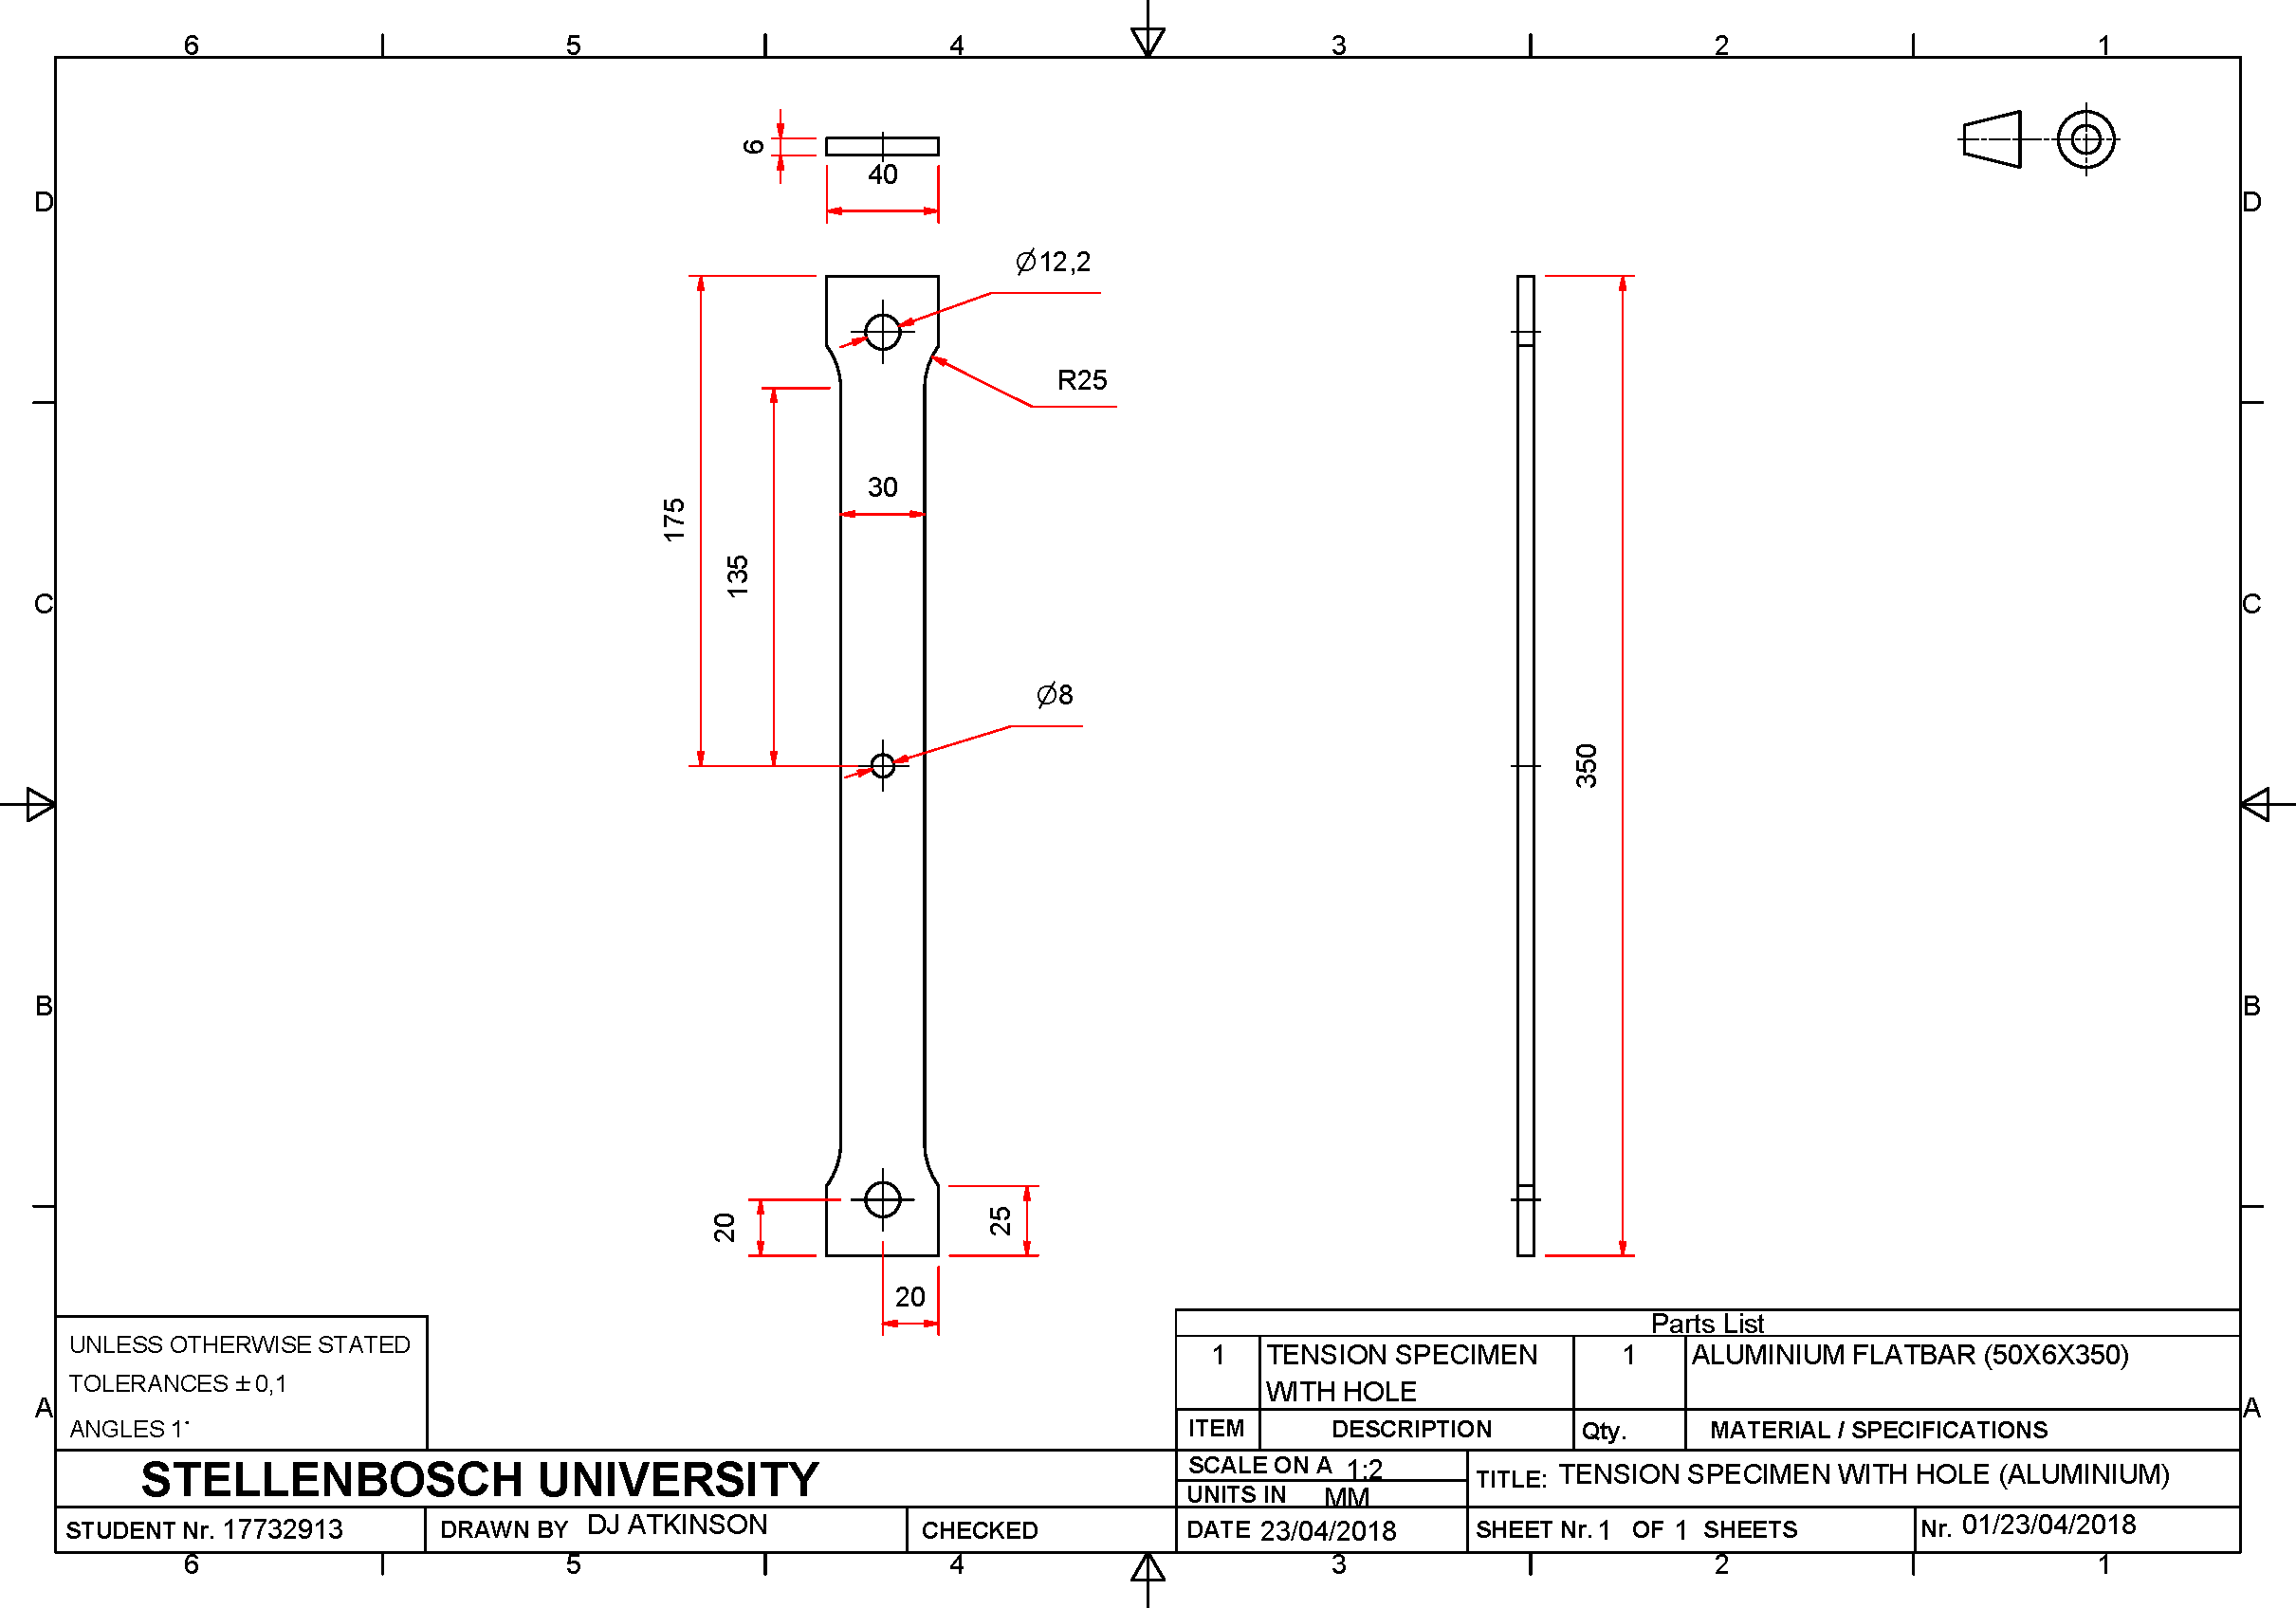
\includegraphics[clip, trim=0.5cm 11cm 0.5cm 11cm, width=1.00\textwidth]{sheet specimen 8mm.pdf}
        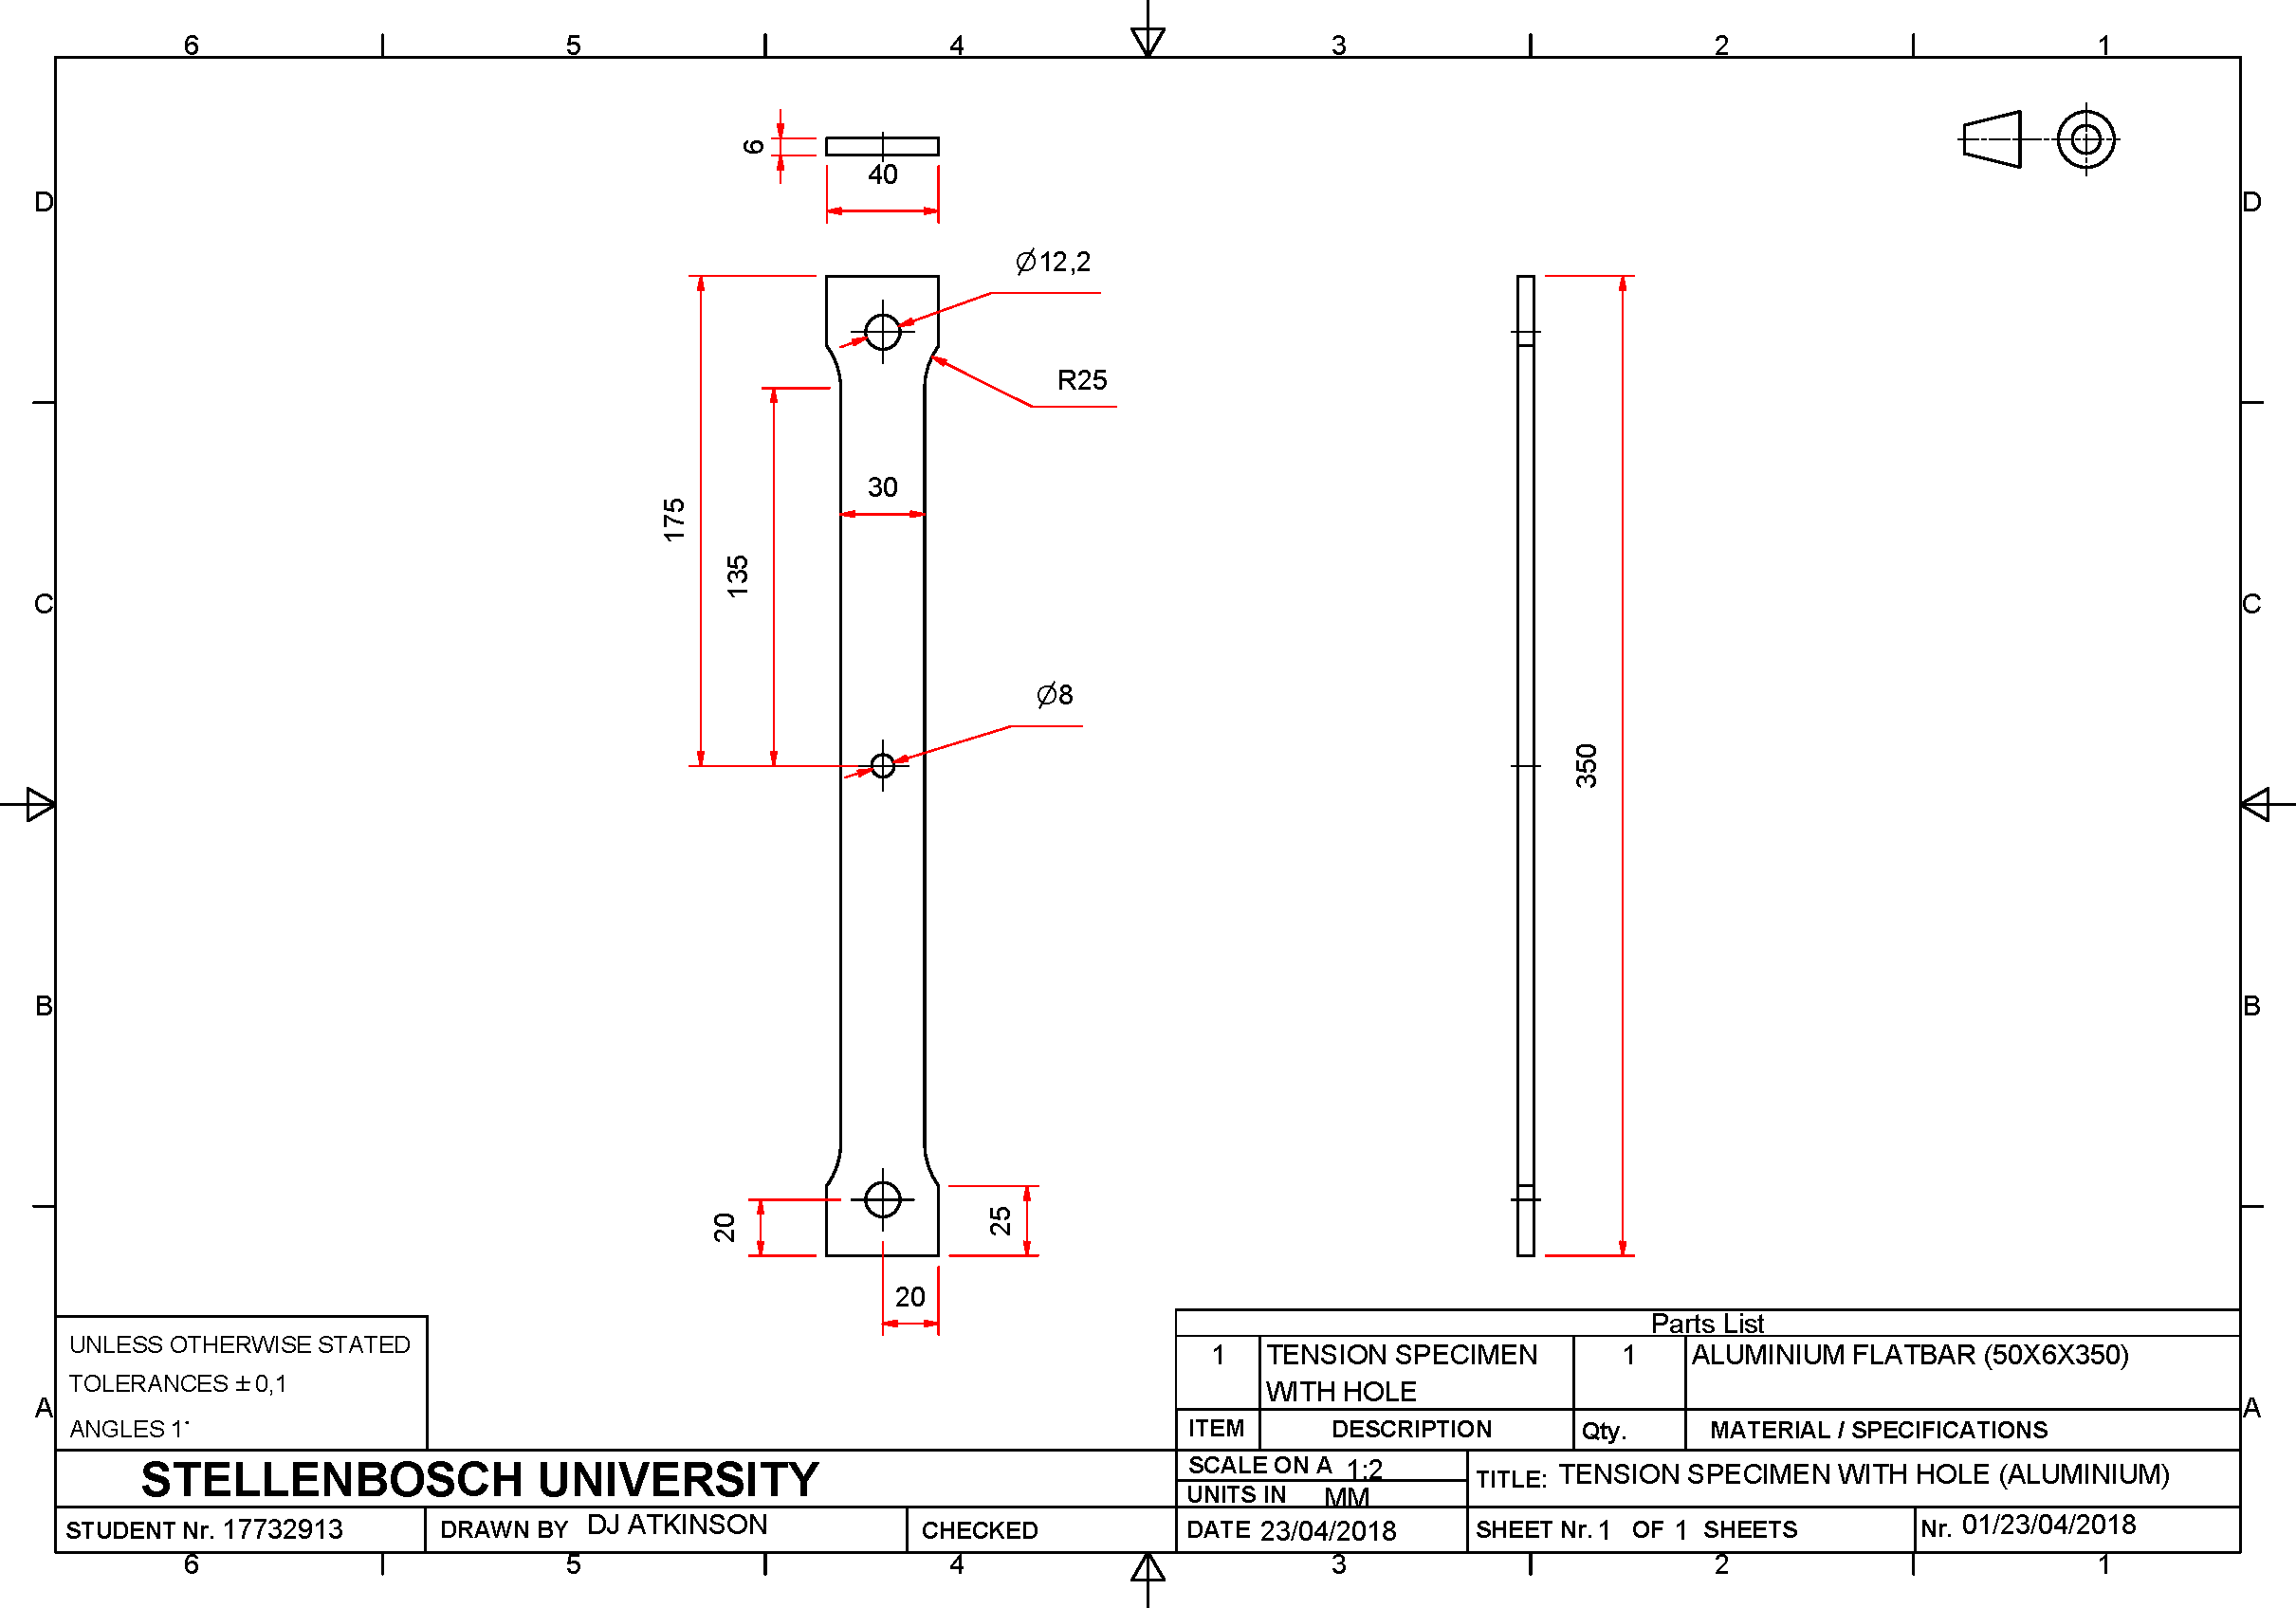
\includegraphics[trim={7cm 6cm 7cm 4.5cm}, clip, scale=0.5]{sheet specimen 8mm.pdf}
    \caption{Tension specimen with hole (I will redo this image such that the specimen lies horizontally so that it takes up less space)}
    \label{fig: tension specimen hole}
\end{figure}
%trim= left lower right upper

\subsubsection{Modified Arcan specimen}
There are many specimen geometries that are designed to investigate the propagation of a crack in the material such as the compact tension specimen, the single-edge-notched bend specimen and the arc-shaped tension specimen \cite{astm2012standard}. However the modified Arcan specimen is unique in that it can investigate pure mode \RomanNumeralCaps{1}, pure mode \RomanNumeralCaps{2} or mixed mode \RomanNumeralCaps{1}-\RomanNumeralCaps{2} crack propagation.

The modified Arcan specimen, shown in Figure \ref{fig: arcan specimen}, and its mounting fixture, shown in Figure \ref{fig: arcan fixture}, were designed according to the guidelines of Banks-Sills and Arcan \cite{banks1986compact} \footnote{These specimens where designed, manufactured and tested by Matthew Molteno and Johan}. These Arcan specimens were laser cut from a 6 mm thick sheet of polymethyl methacrylate (PMMA). PMMA was used because it exhibits linear-elastic brittle fracture so that localised deformation in the vicinity of the crack tip can be minimised. A sharp pre-crack was created in each specimen from the tip of the starter notch, located 15mm from the filleted edge of the specimen, until 20mm from the filleted edge. \todo{si units for length}

\begin{figure}[H]
\centering
\begin{subfigure}[t]{0.45\textwidth}
\centering
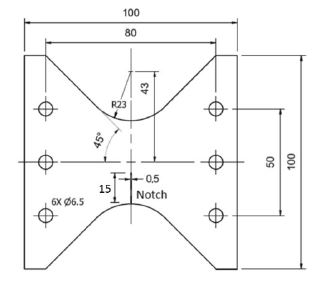
\includegraphics[scale=0.8]{arcan specimen}
\caption{Arcan specimen}
\label{fig: arcan specimen}
\end{subfigure}
\hfill
\begin{subfigure}[t]{0.45\textwidth}
\centering
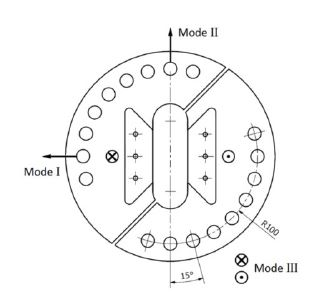
\includegraphics[scale=0.8]{arcan fixture}
\caption{Arcan mounting fixture}
\label{fig: arcan fixture}
\end{subfigure}

\begin{subfigure}[t]{0.45\textwidth}
\centering
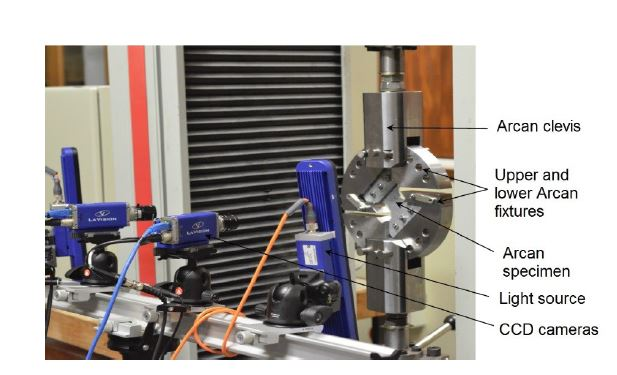
\includegraphics[scale=0.6]{arcan setup}
\caption{Arcan test set up}
\label{fig: arcan setup}
\end{subfigure}
\caption{Arcan components and test setup (these are Matt's images - I will make my own)}
\label{fig: arcan full image}
\end{figure}

The specimen is loaded in the tensile testing machines as shown in Figure \ref{fig: arcan setup} where the specimen is bolted to the two fixture halves and each fixture half is mounted to a clevis using pins through its outer holes. Each fixture half is mounted to a clevis using three pins through its outer holes such that lateral and rotational movement between the two is constrained. The mode of crack propagation is dependent on the angle of the plane of the pre-crack relative to the line of loading of the clevises. Therefore by changing the which holes of the fixture halves are pinned to the clevises this angle can be controlled. The holes for mode \RomanNumeralCaps{1} and mode \RomanNumeralCaps{2} crack propagation are indicated in Figure \ref{fig: arcan fixture}.

The fixture was loaded using an MTS tensile tester with a cross-head speed of 0.25 mm/min. Images were captured at a rate of 1Hz using the LaVision DIC camera system (5MP CCd cameras). 

The reason for including a 
This specimen was chosen so that the subset splitting functionality implemented within the proposed DIC framework can be tested for cracks at different angles \todo{lines of discontinuity at different angles}. As such 





.

.

.

.



how rotate specimen to change mode of loading
designd according to guidelines
origitnal specimen and experiments done by
pictures of them.
why controlling mode is important




% One of the drawbacks of subset based DIC is that it cannot account for discontinuities in the displacement field. However a method of subset splitting has been implemented in the proposed framework to assist with this. 

% The modified Arcan specimen is designed to test the fracture toughness of a material. 

% There are many specimen geometries that are designed to investigate the propagation of a crack in the material however the modified Arcan specimen is unique in that it can investigate pure mode \RomanNumeralCaps{1}, pure mode \RomanNumeralCaps{2} or a mixed mode \RomanNumeralCaps{1} - \RomanNumeralCaps{2} crack propagation.

% it can be mounted in various orientations which  

% There are many specimen geometries that are designed to fail in fracture resulting from the growth of a crack however the modified Arcan specimen is unique in that it can be set up to experience a mixture of modes. 

% The modified Arcan specimen is a butterfly shaped specimen with a precrack along the plane of symmetry. 


% The Arcan specimen, that was originally proposed by Arcan et al. \cite{arcan1978method}, 

% allows a material to be loaded in 



% The arcan specimen was designed to investigate material behaviour under mixed mode (I and II) fracture. It is a symmetric specimen with a precrack at the plane of symmetry. A special type of grip is used for these specimens which allows them to be mounted in various orientations with respect to the force being applied. Thus the plane of the precrack can be adjusted to be at different angles to the direction of the applied force.

% The reason for including this specimen is to test the subset splitting algorithm at various angles.
\subsection{Speckle patterns}
Speckle patterns were applied to the specimens prior to testing. First a base layer of white paint was applied to the specimens over the region of interest of the specimen. Thereafter black speckles were created ontop of this white layer by using a spray can 
















\chapter{Results}
This section provides the results of the Matlab codes in order to prove that it works. The results will be presented here in accordance to the layout of the project sections.

\section{Part A}
Part A dealt with calibration only. The intrinsic parameters determined were
\begin{equation}
  \bm{K} = \begin{bmatrix}
  657.62840 & 0.30335 & 303.72868 & 0\\
  0 & 658.47823 & 245.69177 & 0\\
  0 & 0 & 0 & 0
  \end{bmatrix}.
\end{equation}
The radial distortion parameters were determined to be $k_1 = -0.24885$ and $k_2 = 0.11014$. Using these calibration parameters the image "img01.tiff" was undistorted and is provided in figure \ref{fig:undist1}. Comparing this to the reference image in figure \ref{fig:reference1} it is clear that the calibration parameters determined are sufficiently accurate however differences between the images are noticeable. These differences are likely as a result of additional distortion types that have not been taken into account due to the complexity that these additional distortions would introduce.

\begin{figure}[H]
    \centering
    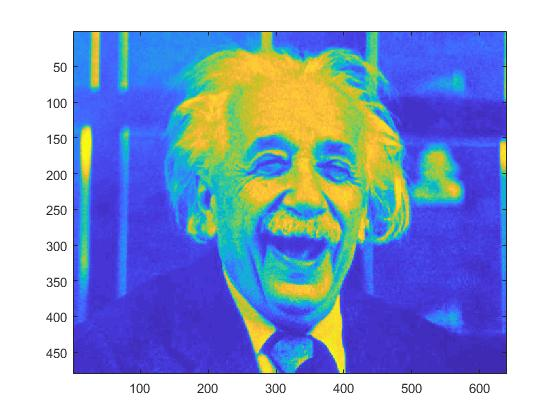
\includegraphics[scale=0.6]{reference_image.jpg}
    \caption{Reference image for comparison purposes}
    \label{fig:reference1}
\end{figure}

\begin{figure}[H]
    \centering
    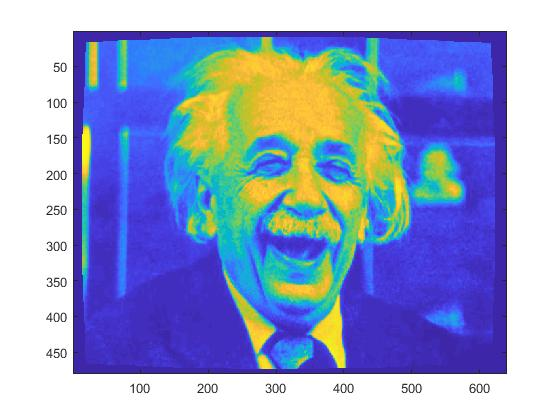
\includegraphics[scale=0.6]{partA.jpg}
    \caption{The distorted image "img01.tiff" which has been corrected for distortions}
    \label{fig:undist1}
\end{figure}

\section{Part B}
Part B deals with the correlation process only. The warp function parameters determined by the Matlab code are presented below.
\begin{align}
  u &= 5.03754\\
  \frac{\partial u}{\partial x} &= 0.04073 \\
  \frac{\partial u}{\partial y} &= -0.02176 \\
  v &= -1.03562 \\
  \frac{\partial v}{\partial x} &= -0.00915 \\
  \frac{\partial v}{\partial y} &= 0.03048
\end{align}
The corresponding correlation coefficients are
\begin{align}
  C_{ZNSSD} &= 0.00587 \\
  C_{ZNCC} &= 0.99706.
\end{align}
Both correlation coefficients have been presented here in order to illustrate that the $C_{ZNCC}$ coefficient is much easier to interpret. The determined warp function parameters were used to undeform the image "img02.tiff" to obtain figure \ref{fig:undist2}. Comparing this to the reference figure in figure \ref{fig:reference2} it can be seen that the determined warp function parameters are sufficiently accurate.

\begin{figure}[H]
    \centering
    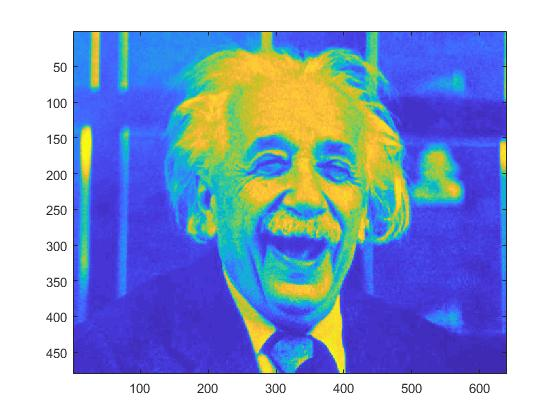
\includegraphics[scale=0.6]{reference_image2.jpg}
    \caption{Reference image for comparison purposes}
    \label{fig:reference2}
\end{figure}

\begin{figure}[H]
    \centering
    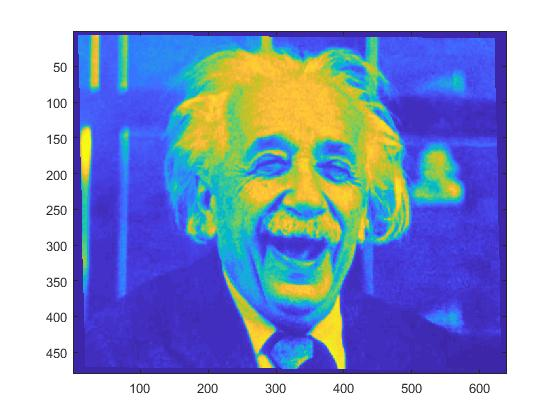
\includegraphics[scale=0.6]{partB.jpg}
    \caption{The distorted image "img02.tiff" which has been corrected for distortions}
    \label{fig:undist2}
\end{figure}
\section{Part C}
Part C combine both Part A and Part B. The calibration code of Part A is used to determine the calibration parameters for the camera system. These camera parameters are then used to undistort image "img03.tif" such that it is free of lens distortion. Then the correlation code is applied to this undistorted image in order to determine the warp function parameters. These warp function parameters are then used to undeform the image. This undeformed image is shown in figure \ref{fig:undist3}. Comparing this image to the original undistorted image in figure \ref{fig:reference3} it seems that the calibration parameters and warp function parameters were sufficiently accurate. However the actual warp function parameters differ from those of Part B as shown below and the correlation coefficient is not as good as in Part B.
\begin{align}
  u &= 5.11364\\
  \frac{\partial u}{\partial x} &= 0.04348 \\
  \frac{\partial u}{\partial y} &= -0.02214 \\
  v &= -1.06509 \\
  \frac{\partial v}{\partial x} &= -0.00918 \\
  \frac{\partial v}{\partial y} &= 0.03071
\end{align}

\begin{align}
  C_{ZNSSD} &= 0.00838 \\
  C_{ZNCC} &= 0.99581
\end{align}

The reason that these warp function parameters differ from those of Part B is that the this method of using the calibration parameters to undistort the image prior to performing correlation on the image is not correct. This is because interpolation is used to undistort the image and additional interpolation is used within the correlation code. 

Thus by introducing an extra case of interpolation the reliability of the data is compromised. This is reflected in the correlation coefficients which differ from those in Part B. Note that the standard deviations of the warp function parameters for both Part B and Part C were on the order of magnitude of $10^{-13}$ sampled over one thousand correlation runs. The calibration parameters for Part C are not presented since they are the same as the values in Part A.

% It is important to note that this method of using the calibration parameters to undistort the image prior to performing correlation on the image is not correct. This is because interpolation is used to undistort the image and additional interpolation is used within the correlation code. Thus by introducing an extra case of interpolation the reliability of the data is compromised.

\begin{figure}[H]
    \centering
    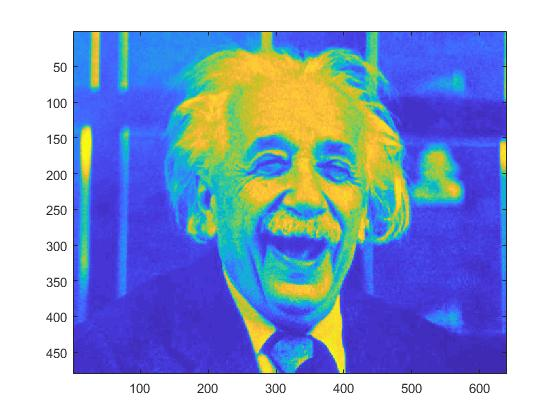
\includegraphics[scale=0.6]{reference_image2.jpg}
    \caption{Reference image for comparison purposes}
    \label{fig:reference3}
\end{figure}

\begin{figure}[H]
    \centering
    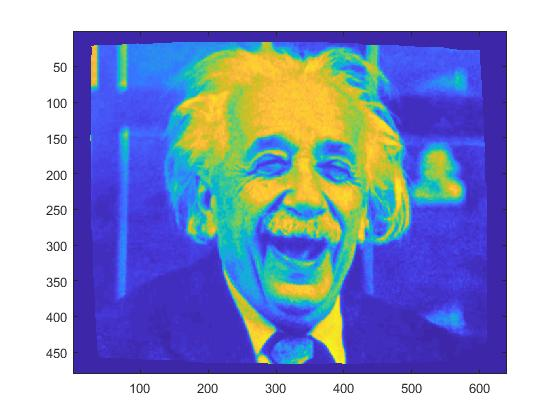
\includegraphics[scale=0.6]{partC.jpg}
    \caption{The distorted image "img03.tiff" which has been corrected for distortions}
    \label{fig:undist3}
\end{figure}

\chapter{Conclusion}
This document outlines the Digital Image Correlation process. It presents the background information on camera optics and the mathematical relation used to model these optics in a camera model. Thereafter the calibration process is discussed which determines the parameter values for the camera model. Correlation is then reviewed with focus on the inverse compositional Lucas-Kanade algorithm. Finally the results of the Matlab codes are given in order to illustrate that the methods presented here are correct.


\bibliography{references}
\bibliographystyle{plain}

\begin{appendices}
\chapter{Code for synthetic image generation}
\label{ap: synthetic image}

\lstinputlisting[language=Matlab]{analyticalspeckleContinuous7_simplified_for_explanation.m}

\chapter{Displacement fields}
\section{Plate with hole}
\label{ap: plate hole}
The displacement equations for a large plate containing a hole have been derived using the Airy stress function as done by Barber in \cite{barber2002solid}. The Airy stress function is a method of using equilibrium equations and boundary conditions of the specimen to solve for the two-dimensional stress and displacement fields experienced by the specimen.

For the case of a large plate with a circular hole in it experiencing a uniform normal stress, $S$, in the x direction the Airy stress function in terms of polar coordinates is
\begin{equation}
  \phi = \frac{Sr^2}{4} - \frac{Sr^2 \cos(2 \theta)}{4} -\frac{Sa^2}{2} + \frac{Sa^2}{2} \cos(2 \theta) - \frac{Sa^4}{4r^2} \cos(2 \theta)
\end{equation}
where $a$ is the radius of the hole. The displacement equations are derived from this by substituting in the appropriate displacement components from the Michell solution \cite{michell1899direct}. After substitution the displacement equations become
\begin{align}
  f_r(r,\theta) &= \frac{1}{2 \mu} \biggl \{ \frac{S}{4} \left[ (k-1)r \right]-\frac{S}{4} \left[ -2r\cos(2\theta) \right] -\frac{Sa^2}{2} \left[ -\frac{1}{r} \right]  \\ 
  &+\frac{Sa^2}{2}\left[ \frac{k+1}{r} \cos(2 \theta)\right] - \frac{Sa^4}{4}\left[ \frac{2}{r^3} \cos(2 \theta) \right] \biggr\} \nonumber \\
  f_{\theta}(r,\theta) &= \frac{1}{2 \mu} \left\{ -\frac{S}{4} \left[ 2r \sin(2 \theta) \right] + \frac{Sa^2}{2}\left[ -\frac{k-1}{r} \sin(2 \theta) \right]- \frac{Sa^4}{4} \left[ \frac{2}{r^3} \sin(2 \theta) \right] \right\}
\end{align}
% \begin{align}
%   2 \mu u_r &= \frac{S}{4} \left[ (k-1)r \right]-\frac{S}{4} \left[ -2r\cos(2\theta) \right] -\frac{Sa^2}{2} \left[ -\frac{1}{r} \right] +\frac{Sa^2}{2}\left[ \frac{k+1}{r} \cos(2 \theta)\right] - \frac{Sa^4}{4}\left[ \frac{2}{r^3} \cos(2 \theta) \right] \\
%   2 \mu u_{\theta} &= -\frac{S}{4} \left[ 2r \sin(2 \theta) \right] + \frac{Sa^2}{2}\left[ -\frac{k-1}{r} \sin(2 \theta) \right]- \frac{Sa^4}{4} \left[ \frac{2}{r^3} \sin(2 \theta) \right]
% \end{align}
where the substituted displacement components are indicated by square brackets. Here $f_r$ is radial displacement, $f_{\theta}$ is angular displacement, $\mu$ is the shear modulus and $k$ is Kolosov's constant. These equations can be converted to describe the displacement in terms of cartesian coordinates using the following equations
\begin{align}
  f_u(r,\theta) = u_r(r,\theta) \cos(\theta) - u_{\theta}(r,\theta) \sin(\theta) \\
  f_v(r,\theta) = u_r(r,\theta) \sin(\theta) + u_{\theta}(r,\theta) \cos(\theta) \\
  \text{where} \quad r=\sqrt{x^2+y^2} \quad \text{and} \quad \theta = \text{atan2} (y,x). \label{eq: pol2cart}
\end{align}



% Further substitution of $\frac{E}{2(1+v)}$ for $\mu$ and $\frac{3-v}{1+v}$ for $k$ (plane stress condition), where $E$ is the elastic modulus and $v$ is Poisson's ratio, gives
% \begin{align}
%   u_r(r,\theta) &= \frac{Sr \cos(2 \theta)}{2E} \left[ 1+v+4\frac{a^2}{r^2} - (1+v)\frac{a^4}{r^4} \right] + \frac{Sr}{2E} \left[ 1-v+(1+v)\frac{a^2}{r^2} \right] \\
%   u_{\theta}(r,\theta) &= - \frac{Sr \sin(2 \theta)}{2E}\left[ 1+v+2(1-v)\frac{a^2}{r^2} + (1+v)\frac{a^4}{r^4} \right]
% \end{align}

% These equations can be converted to describe the displacement in terms of cartesian coordinates using the following equations

Note that atan2 is a Matlab function which computes the arctan of a vector and returns the angle corresponding to the correct quadrant within which that vector lies. The displacement equations in cartesian coordinates become
% \begin{align}
%   u_x(r,\theta) &= \frac{S\,a}{8\,\mu }\left(\frac{2\,a}{r} \left(\cos\left(3\,t\right)+\cos\left(t\right)\,\left(k+1\right)\right)-\frac{2\,a^3}{r^3} \cos\left(3\,t\right)+\frac{r}{a} \cos\left(t\right)\,\left(k+1\right) \right)\\
%   u_y(r,\theta) &= \frac{S\,a}{8\,\mu }\left(\frac{2\,a}{r} \left(\sin\left(3\,t\right)-\sin\left(t\right)\,\left(k-1\right)\right) -\frac{2\,a^3}{r^3} \sin\left(3\,t\right) +\frac{r}{a} \sin\left(t\right)\,\left(k-3\right) \right)
% \end{align}
% Making use of the knowledge that $r=\sqrt{x^2+y^2}$ and $\theta = \text{atan2} (y,x)$ the displacement equations can be rewritten in terms of only cartesian coordinates

\begin{align}
  u_x(x,y,S) &= \frac{S\,a}{8\,\mu } \bigg[\frac{2\,a}{\sqrt{x^2+y^2}} \left(\cos\left(3\,\text{atan2}(y,x) \right)+\cos\left( \text{atan2}(y,x) \right)\,\left(k+1\right)\right) \nonumber \\ &-\frac{2\,a^3}{\left( \sqrt{x^2+y^2} \right) ^3} \cos\left(3\, \text{atan2}(y,x) \right)+\frac{\sqrt{x^2+y^2}}{a} \cos\left( \text{atan2}(y,x) \right)\,\left(k+1\right)  \bigg] \\
  u_y(x,y,S) &= \frac{S\,a}{8\,\mu } \bigg[\frac{2\,a}{\sqrt{x^2+y^2}} \left(\sin\left(3\, \text{atan2}(y,x) \right)-\sin\left( \text{atan2}(y,x) \right)\,\left(k-1\right)\right) \nonumber \\ &-\frac{2\,a^3}{ \left( \sqrt{x^2+y^2} \right)^3} \sin\left(3\, \text{atan2}(y,x) \right) +\frac{\sqrt{x^2+y^2}}{a} \sin\left( \text{atan2}(y,x) \right)\,\left(k-3\right)  \bigg]
\end{align}
where the stress, $S$, has been made a variable of the function.

\section{Plate with crack}
\label{ap: plate crack}
These equations for Cartesian displacements in terms of polar coordinates, for mode \RomanNumeralCaps{1} and \RomanNumeralCaps{2} crack propagation, are of the form \cite{yates2009quantifying}
\begin{align}
  \text{Mode \RomanNumeralCaps{1}:} \nonumber \\
  f_u(r,\theta) &= \sum_{n=1}^{\infty} \frac{r^\frac{n}{2}}{2 \mu} a_n \left[ \left( k+\frac{n}{2} + (-1)^n \right) \cos{\frac{n \theta}{2}} - \frac{n}{2} \cos{\frac{(n-4)\theta}{2}} \right] \\
  f_v(r,\theta) &= \sum_{n=1}^{\infty} \frac{r^\frac{n}{2}}{2 \mu} a_n \left[ \left( k-\frac{n}{2} - (-1)^n \right) \sin{\frac{n \theta}{2}} + \frac{n}{2} \sin{\frac{(n-4)\theta}{2}} \right]\\
  \text{Mode \RomanNumeralCaps{2}:} \nonumber \\
  f_u(r,\theta) &= -\sum_{n=1}^{\infty} \frac{r^\frac{n}{2}}{2 \mu} b_n \left[ \left( k+\frac{n}{2} - (-1)^n \right) \sin{\frac{n \theta}{2}} - \frac{n}{2} \cos{\frac{(n-4)\theta}{2}} \right] \\
  f_v(r,\theta) &= \sum_{n=1}^{\infty} \frac{r^\frac{n}{2}}{2 \mu} b_n \left[ \left( k-\frac{n}{2} + (-1)^n \right) \cos{\frac{n \theta}{2}} + \frac{n}{2} \cos{\frac{(n-4)\theta}{2}} \right]
\end{align}
Using Equation \ref{eq: pol2cart} these equations can be rewritten in purely Cartesian coordinates as
\begin{align}
  \text{Mode \RomanNumeralCaps{1}:} \nonumber \\
  f_u(x,y) &= \sum_{n=1}^{\infty} \frac{(x^2+y^2)^\frac{n}{4}}{2 \mu} a_n \left[ \left( k+\frac{n}{2} + (-1)^n \right) \cos{\frac{n .\text{atan2} (y,x)}{2}} - \frac{n}{2} \cos{\frac{(n-4)\text{atan2} (y,x)}{2}} \right] \\
  f_v(x,y) &= \sum_{n=1}^{\infty} \frac{(x^2+y^2)^\frac{n}{4}}{2 \mu} a_n \left[ \left( k-\frac{n}{2} - (-1)^n \right) \sin{\frac{n .\text{atan2} (y,x)}{2}} + \frac{n}{2} \sin{\frac{(n-4)\text{atan2} (y,x)}{2}} \right]\\
  \text{Mode \RomanNumeralCaps{2}:} \nonumber \\
  f_u(x,y) &= -\sum_{n=1}^{\infty} \frac{(x^2+y^2)^\frac{n}{4}}{2 \mu} b_n \left[ \left( k+\frac{n}{2} - (-1)^n \right) \sin{\frac{n .\text{atan2} (y,x)}{2}} - \frac{n}{2} \cos{\frac{(n-4)\text{atan2} (y,x)}{2}} \right] \\
  f_v(x,y) &= \sum_{n=1}^{\infty} \frac{(x^2+y^2)^\frac{n}{4}}{2 \mu} b_n \left[ \left( k-\frac{n}{2} + (-1)^n \right) \cos{\frac{n .\text{atan2} (y,x)}{2}} + \frac{n}{2} \cos{\frac{(n-4)\text{atan2} (y,x)}{2}} \right]
\end{align}

\end{appendices}
\end{document}




% website for computer vision http://dblp.uni-trier.de/db/journals/ivc/ivc29.html


% Are you a vault dweller, cause you seem pretty S.P.E.C.I.A.L. to me





% https://drive.google.com/uc?export=download&confirm=TXgS&id=0B8ChoAcEOa4HbWxmbGFPV2M0aHM
% https://drive.google.com/uc?export=download&confirm=3xOY&id=0B8ChoAcEOa4HaEljZllabTZaeEk
% https://drive.google.com/uc?export=download&confirm=Lu4C&id=0B8ChoAcEOa4HcHZJMlZLeHdwdnc
% https://drive.google.com/uc?export=download&confirm=Qic1&id=0B2LiEl8up6X_R1V5NkF2NVhwaG8
% https://drive.google.com/uc?export=download&confirm=Qic1&id=0B2LiEl8up6X_R1V5NkF2NVhwaG8
% https://drive.google.com/uc?export=download&confirm=78XC&id=0B_q296AKMRsBUGtORW1jQ0lKQzQ


% https://drive.google.com/uc?export=download&confirm=cxmO&id=0B56v3YurenhzYTRXZGZ6MzJOWnc